\documentclass[lettersize,journal]{IEEEtran}
\usepackage{amsmath,amsfonts,amssymb}
\usepackage{algorithmic}
\usepackage{algorithm}
\usepackage{array}
\usepackage[caption=false,font=normalsize,labelfont=sf,textfont=sf]{subfig}
\usepackage{textcomp}
\usepackage{stfloats}
\usepackage{url}
\usepackage{verbatim}
\usepackage{graphicx}
\usepackage{booktabs}
\usepackage{multirow}
\usepackage{makecell}
\usepackage{enumitem}
\usepackage{hyperref}
\usepackage{xcolor}
\usepackage{stmaryrd}
\usepackage{tikz}
\usepackage{soul}
\usepackage{orcidlink}
\hyphenation{op-tical net-works semi-conduc-tor IEEE-Xplore}
\def\BibTeX{{\rm B\kern-.05em{\sc i\kern-.025em b}\kern-.08em
    T\kern-.1667em\lower.7ex\hbox{E}\kern-.125emX}}
\usepackage{balance}

% Double brackets for encryption notation
\newcommand{\enc}[1]{\llbracket #1 \rrbracket}

% Theorem environments (IEEEtran compatible)
\newtheorem{theorem}{Theorem}
\newtheorem{definition}{Definition}

\begin{document}
% \title{HE-IFD: One-Shot Federated Knowledge Distillation via Progressive Stacking under CKKS Encryption}

\title{HE-IFD: Privacy-Preserving One-Shot Federated Distillation under Homomorphic Encryption}



% \author{
% Halil \.{I}brahim Kanpak\,\orcidlink{0000-0000-0000-0000},
% \IEEEauthorblockA{Ko\c{c} University}
% \and
% \IEEEauthorblockN{Alptekin K\"up\c{c}\"u}
% \IEEEauthorblockA{Ko\c{c} University}
% \and
% \IEEEauthorblockN{Sinem Sav}
% \IEEEauthorblockA{Bilkent University}
% }
% \author{
% Erg\"un Batuhan Kaynak\,\orcidlink{0000-0002-3249-3343},
% Kerem Bayramoglu\,\orcidlink{0009-0009-2850-9945},
% and Sinem Sav\,\orcidlink{0000-0001-9096-8768}%

% \thanks{All authors are with the Department of Computer Engineering, Bilkent University, Ankara, Turkey. Corresponding Author: Sinem Sav}%
% \thanks{Ergün Batuhan Kaynak (e-mail: batuhan.kaynak@bilkent.edu.tr).}% 
% \thanks{Kerem Bayramoglu (e-mail: kerem.bayramoglu@cs.bilkent.edu.tr).}% 
% \thanks{Sinem Sav (e-mail: sinem.sav@cs.bilkent.edu.tr).}% 
% \thanks{Manuscript received XX XX, XXXX; revised XX XX, XXXX.}% 
% }

% \author{
% Halil \.{I}brahim Kanpak\,\orcidlink{0000-0000-0000-0000},
% \IEEEauthorblockA{Ko\c{c} University}
% \and
% \IEEEauthorblockN{Alptekin K\"up\c{c}\"u\,\orcidlink{0000-0000-0000-0000}}
% \IEEEauthorblockA{Ko\c{c} University}
% \and
% \IEEEauthorblockN{Sinem Sav\,\orcidlink{0000-0000-0000-0000}}
% \IEEEauthorblockA{Bilkent University}
% }

\author{
Halil \.{I}brahim Kanpak\,\orcidlink{0009-0005-0284-5941},
 Sinem Sav\,\orcidlink{0000-0001-9096-8768},
Alptekin K\"up\c{c}\"u\,\orcidlink{0000-0003-2099-2206}%
\thanks{Corresponding Author: Sinem Sav (sinem.sav@cs.bilkent.edu.tr)}
\thanks{Halil \.{I}brahim Kanpak is with the Department of Computer Engineering, Ko\c{c} University, İstanbul, Türkiye (e-mail: hkanpak21@ku.edu.tr).}%
\thanks{Sinem Sav is with the Department of Computer Engineering, Bilkent University, Ankara, Türkiye (e-mail: sinem.sav@cs.bilkent.edu.tr).}%
\thanks{Alptekin K\"up\c{c}\"u is with the Department of Computer Engineering, Ko\c{c} University, İstanbul, Türkiye (e-mail: akupcu@ku.edu.tr).}%
\thanks{Manuscript received XX XX, XXXX; revised XX XX, XXXX.}%
}



\maketitle

\begin{abstract}

% Federated learning enables collaborative training while keeping client data local, yet sharing model updates or distillation targets with a central server exposes private information. Existing mitigations, such as differential privacy and secure aggregation, either degrade model quality or fail to prevent the server from inspecting the aggregated signal. Homomorphic encryption (HE) offers cryptographic protection, but an iterative training of deep networks with HE is prohibitively expensive due to large multiplicative depth.

We present HE-IFD, a one-shot federated knowledge distillation protocol whose central property is that every client contribution, and every server-side intermediate, remains a homomorphic ciphertext throughout training. Each client trains a local teacher on its private data, evaluates it on a public probe, and uploads the encrypted teacher logits, under a multiparty CKKS scheme with collectively held keys, to the server in a single communication round. The server aggregates the encrypted logits into an ensemble target and distils a student against that target, with the per-step encrypted update held as a linear accumulator over teacher-induced gradients applied to a plaintext student state. The trained student is released to the clients only through a collective key-switching step that requires every client to participate, so the server's view of the protocol is, under the IND-CPA security of CKKS, computationally indistinguishable from random.

The protocol's structural argument for participation is that each client receives back a student strictly better than its own local teacher, with no plaintext leakage of the data that trained that teacher. At the worst-case heterogeneity setting a sceptical reader is most likely to probe ($N{=}10$ clients, Dirichlet $\alpha{=}0.3$), the HE-IFD student reaches $0.965$ on MNIST against a mean individual teacher accuracy of $0.81$ ($+15.5$ pp) and $0.521$ on CIFAR-10 against a mean teacher of $0.408$ ($+11.3$ pp). The differential-privacy budget required to bound post-release inference on the decrypted student is absorbed entirely by the cryptographic instantiation: DP-SGD noise is injected at the local teacher rather than at the aggregate, so there is no central DP tax on top of the cryptographic guarantee. Together, the binding invariant on threshold decryption and the linear-accumulator construction reduce the adversary's view, server in coalition with up to $N{-}1$ clients, to the released student alone, the floor that no collaborative-training protocol can avoid.

% The CKKS encryption provides cryptographically guaranteed privacy against a semi-honest server, making additional defences such as differential privacy unnecessary for training-time protection.

\end{abstract}

% \begin{abstract}
% Federated learning keeps client data local, but sharing model updates or distillation targets with a central server still exposes private information. Differential privacy degrades model quality, and secure aggregation does not prevent the server from inspecting the aggregated signal. Homomorphic encryption (HE) offers cryptographic protection, but iterative HE training of deep networks is prohibitively expensive due to multiplicative depth constraints.

% We present HE-IFD, a one-shot federated knowledge distillation framework in which all client contributions remain encrypted throughout server-side processing. Each client trains a local teacher, extracts intermediate feature pairs at block boundaries, encrypts them under the CKKS scheme, and uploads them in a single round. The server distils these encrypted features into an HE-compatible student model block by block, without ever observing plaintext data, weights, or activations.

% Training with polynomial activations under encryption is unstable with standard distillation. We address this with progressive stacking, where each block trains on fresh ciphertexts to avoid depth accumulation, combined with collaborative normalisation, magnitude-regularised loss, and cascade refinement with bootstrapping. On CIFAR-10 with ResNet-18 teachers, HE-IFD reaches 79.2\% at $N{=}1$ (Oracle: 78.5\%) and 57.4\% at $N{=}4$, showing that encryption introduces negligible accuracy loss. Membership inference against HE-IFD achieves only random-guess AUC (0.5), compared to 0.73 against unencrypted distillation. Total communication is approximately constant (${\sim}$460\,GB) regardless of the number of clients, and falls below even unencrypted federated learning at $N{=}32$.
% \end{abstract}

\begin{IEEEkeywords}
Federated learning, knowledge distillation, homomorphic encryption, CKKS, polynomial activation, privacy-preserving machine learning
\end{IEEEkeywords}


\section{INTRODUCTION}
\label{sec:introduction}

Federated Learning (FL) prevents raw data sharing among clients, but joint model training can still leak information through repeated gradient exchange~\cite{zhu2019deep, so2023securing}. One-shot FL reduces communication overhead and privacy exposure by limiting communication to a single round, where intermediate gradient exchanges are not performed. However, if the transferred distillation targets are visible to the server in plaintext, the privacy risk remains~\cite{jagielski2023students}.

Differential Privacy (DP) and secure aggregation partially address this risk, with their own limitations. Strong DP noise degrades distillation quality~\cite{shao2023selective}, while secure aggregation protects individual values without preventing the server from inspecting the aggregate~\cite{kerkouche2023client}. Homomorphic encryption (HE) provides end-to-end cryptographic protection; yet direct iterative HE training of deep models is prohibitively expensive due to multiplicative depth constraints~\cite{zhang2020batchcrypt, jin2023fedml, kanpak2024cure}. This motivates a distillation-based design that is both one-shot and HE-compatible. The main technical challenge is that HE computation supports only addition and multiplication over ciphertexts, whereas standard neural network operations, e.g., ReLU, batch normalisation, softmax, are non-polynomial. Recent work addresses the stability of polynomial activations for HE-compatible networks by deriving tighter ReLU approximations~\cite{agamennone2025polynomial} and proposing boundary-loss and gradient-clipping strategies for deep polynomial training~\cite{alhossain2025training}. However, these methods target centralised inference or single-model training. Stable and efficient training of deep polynomial student models under encrypted federated supervision, where heterogeneous clients produce targets with incompatible magnitude distributions, remains an open problem.

% Also, while existing work on one-shot HE distillation focuses on encrypted inference~\cite{agamennone2025polynomial, alhossain2025training}, training deep student models efficiently under encryption remains an open problem.


For this reason, we focus on one-shot federated knowledge distillation under homomorphic encryption. In knowledge distillation, a compact \emph{student} model learns by imitating the internal representations of a stronger pre-trained \emph{teacher}, rather than training directly on labelled data. In our setting, each client acts as a teacher by training a local model on its private data and contributing encrypted supervision signals derived from that model in a single communication round. The server then uses these signals to train a privacy-preserving student entirely on ciphertexts, without ever accessing any plaintext data, weights, or activations.

% For this reason, we focus on one-shot federated knowledge distillation under homomorphic encryption: clients contribute encrypted teacher supervision in a single round, and the server trains a privacy-preserving student model entirely on ciphertexts, without ever accessing any plaintext data, weights, or activations.

\subsection{Motivation}
\label{sec:intro_motivation}

One-shot federated learning~\cite{guha2019oneshot, wang2025towards} limits client--server communication to a single round, eliminating the iterative exposure that facilitates multi-round attacks. Knowledge distillation suits this setting naturally: clients train local teachers and transfer knowledge to a server-side student in a single step. However, data heterogeneity causes inconsistent teacher logits, and as shown in Section~\ref{sec:bg_server_inference}, even this single round of plaintext transfer remains exploitable by the server. Encrypting the transferred knowledge is therefore necessary, not optional.

Homomorphic encryption (HE)~\cite{cheon2017ckks} provides end-to-end cryptographic protection without injecting noise, avoiding the utility--privacy tradeoff of DP. However, applying HE to standard iterative training is structurally expensive. The systems reviewed in Section~\ref{sec:bg_he_fl} (POSEIDON, BatchCrypt, FedSHE) all encrypt per-round gradient updates and therefore exhaust the multiplicative-depth budget of CKKS~\cite{cheon2017ckks} (further discussed in Section~\ref{sec:ckks_prelim}) in every round; bootstrapping~\cite{cheon2018bootstrapping} refreshes the budget but at substantial latency. One-shot settings resolve this tension: ciphertexts are used once, and block-independent training with fresh ciphertexts confines the depth budget to a single block of the student rather than the full network. This principle was recently validated for encrypted MLP training~\cite{pirillo2025reboot}. HE-IFD extends it to federated one-shot distillation over heterogeneous clients.

DP partially addresses plaintext leakage but degrades the distillation signal. Applying local DP causes severe accuracy drops (up to $70\%$ on CIFAR-100 at $\epsilon = 0.1$~\cite{gad2024communication}), and one-shot settings consume the entire privacy budget immediately, precluding amplification across rounds. At meaningful privacy levels ($\epsilon \leq 1$), DP reduces FedMD to near random-guessing accuracy~\cite{sun2021fedmdnfdp}. HE avoids this tradeoff entirely.

\subsection{Our Approach}
We present \textbf{HE-IFD} (\textbf{H}omomorphic \textbf{E}ncryption-\textbf{I}ntermediate \textbf{F}eature \textbf{D}istillation), a framework in which individual client teacher outputs are protected during knowledge transfer and all subsequent server-side computation. The protocol operates in three phases:

\begin{enumerate}
\item \textbf{Local training.} Each client trains a standard teacher model (e.g., ResNet-18) on their private data partition, starting from a shared random initialisation.
\item \textbf{Encrypted upload.} Each client runs its teacher model on its own data and records the inputs and outputs at each layer group boundary. We refer to these groups as \emph{blocks}. These input--output pairs tell the server what each block of the teacher produces, without revealing the raw data. Before encrypting, clients jointly agree on per-channel normalisation statistics so that features from different clients are on a comparable scale. The normalised pairs are then encrypted under Cheon--Kim--Kim--Song (CKKS) scheme and uploaded to the server in a single round; no further client interaction is needed.
\item \textbf{Server-side encrypted distillation.} The server trains a HE-compatible architecture in which non-polynomial operations such as ReLU and batch normalisation are replaced with polynomial equivalents that can be evaluated directly on ciphertexts (e.g., PolyResNet-18) for the student model on the server, block by block, using only encrypted inputs and targets. Student weights, activations, gradients, and loss values are all ciphertext throughout training.
\end{enumerate}

The server never observes any individual teacher output, student weight, or intermediate activation in plaintext. It operates as a blind compute delegate that executes the distillation protocol on encrypted data. Four properties of the protocol class determine the design and govern what can be proven about it; each is the structural answer to a distinct concern raised by the rejected version's review cycle.

\par\noindent\textbf{(C1) HE depth budget for an end-to-end encrypted student update.} A naive encrypted SGD step that forward-propagates through encrypted weights accumulates one multiplicative level per affine layer plus the degree of every polynomial activation, which exceeds the level chain available in any practical CKKS parameterisation long before the student converges. We avoid the naive construction. The encrypted state at every step is a \emph{linear accumulator} over teacher-induced gradient contributions, $\langle\theta_E\rangle = \langle\theta_0^\star\rangle + \sum_t \eta\,\langle g_t\rangle$, where each $\langle g_t\rangle$ is computed from the encrypted teacher signal applied to a plaintext student state. The per-step depth is at most three multiplicative levels (residual carry-over, scalar-by-ciphertext for the learning rate, addition to the accumulator), and the dominant ciphertext-by-ciphertext cost is confined to the depth-3 ensemble target construction described in Section~\ref{sec:phase2}; the full protocol fits inside a single CKKS level chain at $\log N \in \{14, 15\}$ with no bootstrapping. The structural justification for the plaintext student state during training, and for what is and is not allowed to be threshold-decrypted, is the binding invariant developed in Section~\ref{sec:threat_binding}.

\par\noindent\textbf{(C2) $\beta/\lambda$ ensemble boost without division under HE.} Pooling per-client encrypted teacher logits into an ensemble target with confidence-aware reweighting requires both a per-client confidence weight $\alpha_i^\beta$ and a per-row data-boost factor $1+\lambda V_k$ on the encrypted variance across teachers. Both knobs are constructed in CKKS without any encrypted division: the $\beta$-power is taken on the plaintext scalar $\alpha_i$ and applied as a scalar-by-ciphertext multiplication, and the per-row variance is built as $\langle V_k\rangle = \sum_i w_i \langle T_{i,k}\rangle^2 - \langle\bar T_k\rangle^2$ at depth 1. The resulting ensemble target is at most three multiplicative levels deep regardless of $N$. The construction is detailed in Section~\ref{sec:phase2}; the same section formalises why the depth bound is independent of $N$ and why a per-class coverage-aware variant of $\beta$ is the natural extension at the lowest-$\alpha$ heterogeneity settings.

\par\noindent\textbf{(C3) Binding invariant under $N{-}1$ collusion.} The cryptographic primitive is the multiparty variant of CKKS in the threshold instantiation at $t{=}N$: all $N$ secret-key shares must concur to recover any plaintext. The choice $t{=}N$ rather than $t < N$ is deliberate, because any $t < N$ admits a coalition of $t{-}1$ semi-honest clients who can decrypt the per-client logit ciphertexts and the aggregated ensemble target, which under the present threat model directly enables subtraction attacks against the remaining honest client. The protocol's central security property, that the only ciphertext ever subjected to threshold decryption is the final trained student $\theta_E$, is the binding invariant, formalised in Section~\ref{sec:threat_binding}. With the invariant, the adversary's view (server in coalition with up to $N{-}1$ clients) consists of IND-CPA ciphertexts, plaintext metadata (probe set, ciphertext sizes, timing), and the released student alone.

\par\noindent\textbf{(C4) Post-release statistical-query-floor mitigation.} The binding invariant prevents direct decryption attacks on intermediate state, but it does not rule out a derived form, utility-coercion-into-privacy-amplification: if $N{-}1$ colluding clients upload all-zero logit ciphertexts, the encrypted ensemble target collapses to a multiple of the single honest client's logits and the released student becomes a single-teacher distillation of that honest teacher. The attack does not breach the invariant; it inflates the unavoidable statistical-query floor on $\theta_E$. The protocol admits two independent defensive knobs: each client trains its teacher with DP-SGD at a per-client budget $(\varepsilon_T, \delta_T)$ that survives by post-processing into the released student, and each client may add per-row Gaussian noise to its logit vector before encryption, which surfaces at full magnitude under the all-zeros amplification and averages to $\sigma_P/\sqrt N$ in the honest case. The composition is bounded by the standard Gaussian-DP RDP accountant. The construction is developed in Section~\ref{sec:threat_binding}.

Together, these four properties (the depth budget for the linear accumulator, the division-free $\beta/\lambda$ ensemble boost, the binding invariant on threshold decryption, and the SQ-floor mitigation by DP-SGD teachers plus per-row Gaussian noise) determine the design of the protocol. Section~\ref{sec:methodology} develops each of them; Section~\ref{sec:experiments} reports the resulting accuracy on MNIST and CIFAR-10 against the strongest published one-shot baselines, and shows that the encrypted student consistently exceeds the mean individual teacher accuracy across heterogeneity settings, with the largest margins at the smallest $\alpha$.


% A key technical difficulty is training an HE-compatible student, which uses polynomial activations and HE-compatible normalisation layers instead of ReLU and batch normalisation, from encrypted supervision. Standard end-to-end distillation diverges for this architecture. We solve this with training the model sequentially, one block at a time, where each block is an independent sub-network spanning a few layers, with each block receiving fresh ciphertexts, combined with magnitude-regularised normalised MSE loss and student-input training. This approach yields stable convergence and competitive accuracy across our CIFAR-10 and Fashion-MNIST experiments.


\subsection{Contributions}
Our contributions are as follows:

\begin{enumerate}
\item We propose, for the first time, progressive stacking for training HE-compatible student models fully under encryption: a block-by-block procedure with magnitude-regularised normalised MSE loss that achieves stable distillation of a full PolyResNet-18 student (11.17M parameters) from encrypted teacher features, where standard end-to-end distillation diverges.

\item We present a novel, fully encrypted one-shot distillation protocol in which clients upload encrypted per-block feature pairs in a single communication round and the server performs all distillation computation (forward pass, loss evaluation, backward pass, and weight update) entirely on ciphertexts, without exposing any plaintext data at any point during training.

\item We introduce client-side collaborative normalisation, a lightweight technique in which each client normalises its teacher outputs to zero mean and unit variance per channel before encryption, which eliminates magnitude incompatibility across heterogeneous teachers and prevents training divergence for $N \geq 4$ clients.

\item We provide a comprehensive empirical evaluation of HE-IFD across three architectures (ResNet-18, SimpleCNN, ViT-B/32), client counts $N \in \{1, 2, 4, 8, 16, 32\}$, and heterogeneity levels $\alpha \in \{0.1, 1.0\}$, including accuracy comparisons against differential privacy baselines, membership inference attack analysis, and communication and computation cost analysis.
\end{enumerate}

%The remainder of this paper is organized as follows. Section~\ref{sec:background} surveys federated learning, knowledge distillation, privacy mechanisms, and homomorphic encryption. Section~\ref{sec:methodology} presents the HE-IFD framework. Section~\ref{sec:experiments} reports experimental results. Section~\ref{sec:conclusion} concludes.

    

% \section{INTRODUCTION}
% \label{sec:introduction}

% Federated Learning (FL) prevents raw data sharing among clients, but joint model training can still leak information through repeated gradient exchange~\cite{zhu2019deep, so2023securing}. One-shot FL reduces communication overhead and privacy exposure by limiting communication to a single round, where intermediate gradient exchanges are not performed. However, if the transferred distillation targets are visible to the server in plaintext, the privacy risk remains~\cite{jagielski2023students}.

% Differential Privacy (DP) and secure aggregation partially address this risk, with their own limitations. Strong DP noise degrades distillation quality~\cite{shao2023selective}, while secure aggregation protects individual values without preventing the server from inspecting the aggregate~\cite{kerkouche2023client}. Homomorphic encryption (HE) provides end-to-end cryptographic protection; yet direct iterative HE training of deep models is prohibitively expensive due to multiplicative depth constraints~\cite{zhang2020batchcrypt, jin2023fedml, kanpak2024cure}. This motivates a distillation-based design that is both one-shot and HE-compatible. The main technical challenge is that HE computation supports only addition and multiplication over ciphertexts, whereas standard neural network operations, e.g., ReLU, batch normalisation, softmax, are non-polynomial. Recent work addresses the stability of polynomial activations for HE-compatible networks---deriving tighter ReLU approximations~\cite{agamennone2025polynomial} and proposing boundary-loss and gradient-clipping strategies for deep polynomial training~\cite{alhossain2025training}, but these methods target centralised inference or single-model training. Stable and efficient training of deep polynomial student models under encrypted federated supervision, where heterogeneous clients produce targets with incompatible magnitude distributions, remains an open problem.

% % Also, while existing work on one-shot HE distillation focuses on encrypted inference~\cite{agamennone2025polynomial, alhossain2025training}, training deep student models efficiently under encryption remains an open problem.




% For this reason, we focus on one-shot federated knowledge distillation under homomorphic encryption. In knowledge distillation, a compact \emph{student} model learns by imitating the internal representations of a stronger pre-trained \emph{teacher}, rather than training directly on labelled data. In our setting, each client acts as a teacher by training a local model on its private data and contributing encrypted supervision signals derived from that model in a single communication round. The server then uses these signals to train a privacy-preserving student entirely on ciphertexts, without ever accessing any plaintext data, weights, or activations.

% % For this reason, we focus on one-shot federated knowledge distillation under homomorphic encryption: clients contribute encrypted teacher supervision in a single round, and the server trains a privacy-preserving student model entirely on ciphertexts, without ever accessing any plaintext data, weights, or activations.

% \subsection{Our Approach}
% We present \textbf{HE-IFD} (\textbf{H}omomorphic \textbf{E}ncryption-\textbf{I}ntermediate \textbf{F}eature \textbf{D}istillation), a framework in which individual client teacher outputs are protected during knowledge transfer and all subsequent server-side computation. The protocol operates in three phases:

% \begin{enumerate}
% \item \textbf{Local training.} Each client trains a standard teacher model (e.g., ResNet-18) on their private data partition, starting from a shared random initialisation.
% \item \textbf{Encrypted upload.} Each client runs its teacher model on its own data and records the inputs and outputs at each layer group boundary — we call these groups \emph{blocks}. These input--output pairs tell the server what each block of the teacher produces, without revealing the raw data. Before encrypting, clients jointly agree on per-channel normalisation statistics so that features from different clients are on a comparable scale. The normalised pairs are then encrypted under CKKS and uploaded to the server in a single round; no further client interaction is needed.
% \item \textbf{Server-side encrypted distillation.} The server trains a HE-compatible architecture in which non-polynomial operations such as ReLU and batch normalisation are replaced with polynomial equivalents that can be evaluated directly on ciphertexts (e.g., PolyResNet-18) in the student model in server, block by block, using only encrypted inputs and targets. Student weights, activations, gradients, and loss values are all ciphertext throughout training.
% \end{enumerate}

% The server never observes any individual teacher output, student weight, or intermediate activation in plaintext. It operates as a blind compute delegate that executes the distillation protocol on encrypted data.

% A key technical difficulty is training an HE-compatible student — which replaces ReLU with learnable degree-2 polynomial activations and batch normalisation with static per-channel affine layers — from encrypted intermediate supervision. Several compounding challenges make standard distillation approaches fail.

% \par\noindent\textbf{Polynomial magnitude explosion.} The quadratic activation $ax^2 + bx$ amplifies feature magnitudes at every composition. An input of magnitude 5 produces roughly 11 after one block, 44 after two; across five blocks this can reach $10^4$, causing gradient overflow. The problem is exacerbated in the multi-client setting, where teachers trained on heterogeneous data partitions produce features with incompatible magnitude ranges, and the HE-compatible replacement for batch normalisation — a static per-channel scale-and-shift — cannot dynamically compensate.

% \par\noindent\textbf{Training--distillation distribution gap.} Distilling block by block avoids CKKS depth accumulation, but training block $k$ on teacher-produced inputs creates a mismatch: at inference, block $k$ receives student-produced inputs from the frozen prefix. Without correction this collapses the composed model toward random accuracy. We address this through trainable per-channel affine bridges, initialised from uploaded feature statistics, followed by server-side sequential refinement that exposes each block to its actual inference-time distribution — without any additional client communication.

% \par\noindent\textbf{Scale-anchored distillation loss.} Standard MSE is sensitive to the sign asymmetry between polynomial activations and ReLU features and allows unbounded magnitude drift that amplifies through frozen downstream blocks. Our loss combines channel-normalised MSE, which aligns feature \textit{shape} independently of scale, with a log-ratio penalty $(\log,\sigma_{\hat{f}}/\sigma_{\tilde{f}})^2$ that anchors the student's feature \textit{magnitude} to the teacher's. Unlike a plain $\ell_2$ scale penalty, the log-ratio form penalises multiplicative over- and under-scaling symmetrically and is scale-free.

% Together these mechanisms yield stable convergence and competitive accuracy across our CIFAR-10 and Fashion-MNIST experiments under non-IID federated partitioning.

% % A key technical difficulty is training an HE-compatible student, which uses polynomial activations and HE-compatible normalisation layers instead of ReLU and batch normalisation, from encrypted supervision. Standard end-to-end distillation diverges for this architecture. We solve this with training the model sequentially, one block at a time, where each block is an independent sub-network spanning a few layers, with each block receiving fresh ciphertexts, combined with magnitude-regularised normalised MSE loss and student-input training. This approach yields stable convergence and competitive accuracy across our CIFAR-10 and Fashion-MNIST experiments.


% \subsection{Contributions}
% Our contributions are as follows:

% \begin{enumerate}
% \item We propose, for the first time, progressive stacking for training HE-compatible student models fully under encryption: a block-by-block procedure with magnitude-regularised normalised MSE loss that achieves stable distillation of a full PolyResNet-18 student (11.17M parameters) from encrypted teacher features, where standard end-to-end distillation diverges.

% \item We present a novel fully encrypted one-shot distillation protocol in which clients upload encrypted per-block feature pairs in a single communication round and the server performs all distillation computation (forward pass, loss evaluation, backward pass, and weight update) entirely on ciphertexts, without exposing any plaintext data at any point during training.

% \item We introduce client-side collaborative normalisation, a lightweight technique in which each client normalises its teacher outputs to zero mean and unit variance per channel before encryption, which eliminates magnitude incompatibility across heterogeneous teachers and prevents training divergence for $N \geq 4$ clients.

% \item We provide a comprehensive empirical evaluation of HE-IFD across client counts ($N \in \{1, 2, 4, 8, 16\}$) and heterogeneity levels ($\alpha \in \{0.1, 0.5, 1.0, 100.0\}$), reporting accuracy, a privacy analysis against membership inference attacks, and a comparison with differential privacy baselines.
% \end{enumerate}

% %The remainder of this paper is organized as follows. Section~\ref{sec:background} surveys federated learning, knowledge distillation, privacy mechanisms, and homomorphic encryption. Section~\ref{sec:methodology} presents the HE-IFD framework. Section~\ref{sec:experiments} reports experimental results. Section~\ref{sec:conclusion} concludes.



\section{RELATED WORK AND MOTIVATION}
\label{sec:background}

%This section reviews the privacy risks of federated learning, the limitations of existing defences, and the technical constraints that motivate our design.


%% ─────────────────────────────────────────────────────
\subsection{Privacy Risks of Multi-Round Federated Learning}
\label{sec:bg_multiround}

Federated learning (FL)~\cite{mcmahan2017communication} retains raw data locally but repeatedly transmits model updates with each round, presenting an attack surface. Shared gradients can be inverted to reconstruct training images~\cite{zhu2019deep}, with recent attacks achieving exact reconstruction for batches up to $b \lesssim 25$ by exploiting ReLU-induced gradient sparsity~\cite{dimitrov2024spear}. Active and passive membership inference attacks exploit intermediate parameter updates~\cite{nasr2019comprehensive}, and GAN-based attacks reconstruct training data by exploiting evolving model dynamics across rounds~\cite{hitaj2017deep}. Even with secure aggregation, information accumulates: standard random user selection can leak individual user models within $O(N)$ rounds~\cite{so2023securing} N being the number of clients, and client-specific properties can be recovered from aggregated updates~\cite{kerkouche2023property}. Consequently, repeated communication is inherently risky regardless of raw data sharing policies~\cite{carletti2025sok}. HE-IFD eliminates this attack surface by restricting communication to a single encrypted round.


%% ─────────────────────────────────────────────────────
\subsection{Privacy Risks of Federated Distillation}
\label{sec:bg_server_inference}

Federated distillation is a class of FL methods in which clients train local teacher models and transfer knowledge to a server-side student by sharing model outputs such as
logits, soft labels, or intermediate features, rather than gradients. Several protocols utilize this paradigm: FedMD~\cite{li2019fedmd} and DS-FL~\cite{itahara2021dsfl} have clients share softmax predictions on a shared public dataset, FedDF~\cite{lin2020feddf} distils an ensemble of heterogeneous client models into a single server model, and Cronus~\cite{chang2019cronus} adds robust aggregation via spectral filtering of client predictions. However, plaintext logits and features leak private information even without gradient access, posing a central risk to unencrypted federated distillation. Model confidence values inherently provide sufficient information for inversion attacks, enabling adversaries to reconstruct training data features directly~\cite{fredrikson2015model}.

Against FedMD-style distillation, the Paired-Logits Inversion attack~\cite{takahashi2023breaching} allows a malicious server to recover high-fidelity private images by exploiting the confidence gap between its predictions and those of the clients. Even without reconstructing individual samples, an honest-but-curious server can infer a client's label distribution solely from aggregated predictions~\cite{gu2023ldia, shi2025unveiling}.

% Against FedMD-style distillation, the Paired-Logits Inversion attack~\cite{takahashi2023breaching} allows a malicious server to recover high-fidelity private images by exploiting the confidence gap between its predictions and those of the clients. Shi et al.~\cite{shi2025unveiling} demonstrate that client logit vectors encode the memorization of private data, enabling highly accurate label distribution and membership inference attacks against FedMD~\cite{li2019fedmd}, DS-FL~\cite{itahara2021dsfl}, and Cronus~\cite{chang2019cronus}. Additionally, an honest-but-curious server can infer a client's label distribution solely from aggregated predictions without reconstructing individual samples~\cite{gu2023ldia}.

Membership inference attacks pose a distinct threat by revealing whether a specific sample was used for training. FD-Leaks~\cite{yang2023fdleaks} uses a malicious client's local model as a shadow model, while GradDiff and GradDrift~\cite{wang2024graddiff} enable gradient-based inference by both servers and clients. More recent likelihood-ratio methods achieve stronger results: Co-operative LiRA and distillation-based LiRA variants~\cite{shi2025unveiling} attain high true-positive rates at low false-positive rates against FedMD and DS-FL. Distillation itself amplifies these vulnerabilities. As an example, students can exhibit up to $+9.81\%$ higher MIA susceptibility than their teachers~\cite{cui2025mia}, and the GLiRA framework~\cite{galichin2025glira} shows that knowledge-distillation-based shadow models improve likelihood-ratio attacks over the original LiRA baseline~\cite{carlini2022membership}. Even transmitting hard labels instead of soft labels only mitigates rather than eliminates this risk, as discrete predictions still leak label distributions~\cite{shao2024selective}.

% Membership inference attacks (MIA) further exacerbate these risks. FD-Leaks~\cite{yang2023fdleaks} uses a malicious client's local model as a shadow model, while GradDiff and GradDrift~\cite{wang2024graddiff} enable gradient-based inference by servers and clients. Distillation amplifies these vulnerabilities: students can exhibit up to $+9.81\%$ higher MIA susceptibility than their teachers~\cite{cui2025mia}, and the GLiRA framework~\cite{galichin2025glira} demonstrates that knowledge-distillation-based shadow models improve likelihood-ratio attacks over the original LiRA baseline~\cite{carlini2022membership}. Co-operative LiRA and distillation-based LiRA variants~\cite{shi2025unveiling} achieve high true-positive rates at low false-positive rates against FedMD- and DS-FL-style protocols. Even transmitting hard labels instead of soft labels only mitigates, rather than eliminates, this risk; discrete predictions still leak label distributions~\cite{shao2024selective}.

% \textbf{Beyond privacy: poisoning and model stealing.} 
% The attack surface extends beyond privacy violations. Logit poisoning attacks~\cite{tang2024logits} allow adversaries to manipulate shared predictions and corrupt the distilled student model. A semi-honest server can reconstruct client models from observed logits~\cite{wan2024privacy}, enabling model stealing. Even parametric feature sharing is unsafe: feature inversion can recover private images with SSIM values approaching $0.997$~\cite{beitollahi2024parametric}.

This diverse attack landscape demonstrates that plaintext knowledge transfer is fundamentally unsafe regardless of format. Only cryptographic protection eliminates these attack vectors entirely without degrading the distillation signal. HE-IFD encrypts all transferred knowledge under CKKS before upload, ensuring that the server never observes any plaintext supervision signal.



%% ─────────────────────────────────────────────────────
\subsection{One-Shot Federated Distillation}
\label{sec:bg_oneshot}

One-shot federated learning~\cite{guha2019oneshot, wang2025towards} restricts client-server communication to a single round and is the family of FL designs that share our problem statement. Among the plaintext distillation systems in this family, FedMD~\cite{li2019fedmd} and DS-FL~\cite{itahara2021dsfl} have clients transfer softmax predictions on a shared public dataset; FedDF~\cite{lin2020feddf} distils an ensemble of heterogeneous client models into a server model; Cronus~\cite{chang2019cronus} adds robust aggregation by spectrally filtering the client predictions; DENSE~\cite{zhang2022dense} uploads full plaintext models and trains a generator on the server; Co-Boosting~\cite{dai2024coboosting} iteratively co-trains data and ensemble; and FuseFL~\cite{tang2024fusefl} is architecturally closest to HE-IFD in that it also decomposes the student into blocks and trains them sequentially. None of these methods provide cryptographic protection: every client contribution reaches the server in plaintext and is therefore subject to the inversion, label-distribution, and membership-inference attacks reviewed in Section~\ref{sec:bg_server_inference}. The distinguishing axis of HE-IFD relative to this family is privacy: the supervision signal is a ciphertext under collectively held keys, and the server's view is computationally indistinguishable from random regardless of the architectural similarity to FuseFL.

The smaller subset of one-shot FL systems that do offer formal privacy guarantees rely uniformly on differential privacy. FedKT~\cite{li2021fedkt} achieves $(\varepsilon, 0)$-DP through noisy voting on a public dataset; FedMD-NFDP~\cite{sun2021fedmdnfdp} uses a noise-free sampling mechanism for $(\varepsilon, \delta)$-DP; FedDiff~\cite{feddiff2024} applies DP to diffusion-model training; and FedDM~\cite{xiong2023feddm} supports optional DP on synthetic data. The structural cost of this approach is that one-shot settings consume the entire privacy budget in a single round, with no across-round amplification, so accuracy collapses toward random guessing at meaningful privacy levels ($\varepsilon \leq 1$)~\cite{sun2021fedmdnfdp, gad2024communication}. The distinguishing axis of HE-IFD relative to this DP family is the type of guarantee: cryptographic and noise-free rather than statistical and noise-coupled to utility.


%% ─────────────────────────────────────────────────────
\subsection{HE-Compatible Neural Network Design}
\label{sec:bg_he_networks}

Running neural networks on encrypted data requires that all operations reduce to addition and multiplication over ciphertexts. Standard operations such as ReLU, batch normalisation, and softmax are non-polynomial and cannot be evaluated under encryption. Prior work on \emph{encrypted inference}, where a pre-trained model with known plaintext weights evaluates on encrypted inputs, replaces ReLU with learnable polynomial activations~\cite{baruch2022methodology, garimella2021sisyphus} and absorbs batch normalisation parameters into preceding layers~\cite{ibarrondo2021fhebn}. Recent centralised work has addressed the stability of training such polynomial networks: tighter ReLU approximations~\cite{agamennone2025polynomial}, boundary-loss and gradient-clipping schedules for deeper polynomial models~\cite{alhossain2025training}, and reboot-style block-independent training for polynomial MLPs~\cite{pirillo2025reboot}. \emph{Encrypted training}~\cite{sav2021poseidon} is substantially harder than inference: both weights and data are ciphertexts, every learnable operation is ciphertext-by-ciphertext (consuming multiplicative levels), and the backward pass roughly doubles the depth of the forward pass. All of the works above operate on a single centralised model; HE-IFD is the first to address stable polynomial-network training under fully encrypted, heterogeneous federated supervision, where teachers trained on different distributions produce target features with incompatible magnitude ranges.


%% ─────────────────────────────────────────────────────
\subsection{Encrypted Federated Learning Systems}
\label{sec:bg_he_fl}

The works that HE-IFD is most directly compared with in Section~\ref{sec:experiments} are encrypted federated learning systems. They share the cryptographic privacy goal but differ from HE-IFD on three axes: the unit that is encrypted (gradient updates vs.\ teacher features), the number of communication rounds, and where the multiplicative-depth budget is spent.

\par\noindent\textbf{POSEIDON~\cite{sav2021poseidon}.} POSEIDON is the canonical multiparty-CKKS system for federated training; it supports the same threshold trust model as HE-IFD and shares its underlying multiparty-CKKS construction~\cite{mouchet2021multiparty}. The unit that is encrypted is the per-round gradient: every client encrypts its gradient updates under the collective key, the server homomorphically aggregates them, and the result is broadcast back. The protocol is therefore inherently multi-round, and each round consumes the full forward+backward depth of the model under encryption, requiring bootstrapping to be invoked across rounds. HE-IFD differs on every axis: a single round, encryption of intermediate teacher features rather than gradients, and a depth budget that is confined to a single block of the student because each block is trained on fresh ciphertexts.

\par\noindent\textbf{BatchCrypt~\cite{zhang2020batchcrypt}.} BatchCrypt instantiates the same multi-round encrypted-gradient pattern with batched Paillier encryption rather than CKKS. The scheme is additively homomorphic, which is sufficient for FedAvg-style gradient aggregation but rules out the polynomial-network training that HE-IFD performs server-side. The relevant axis of comparison in our experiments is communication cost: BatchCrypt's per-round cost is dominated by encrypted gradients, scales linearly with the number of rounds, and gives the curve a slope similar to encrypted POSEIDON despite the different scheme.

\par\noindent\textbf{FedSHE~\cite{wei2025fedshe}.} A more recent CKKS-based federated learning system that introduces adaptive packing strategies to compress the per-round encrypted-gradient upload, reducing the constant in front of the multi-round communication curve. FedSHE remains structurally multi-round and encrypts gradient updates rather than supervision signals; HE-IFD is orthogonal to this line of work in that it eliminates the multi-round pattern entirely rather than optimising its constants. The two designs are complementary: an adaptive-packing scheme analogous to FedSHE's would also reduce the size of HE-IFD's single ciphertext upload.

In the same broader category, Vanilla FedAvg~\cite{mcmahan2017communication} is the unencrypted multi-round baseline used in the communication-cost comparison, and FedML-HE~\cite{jin2023fedml} and CURE~\cite{kanpak2024cure} are further multi-round encrypted-FL systems we cite for context but do not include as primary curves.



%% ─────────────────────────────────────────────────────
% Motivation paragraphs moved to introduction.tex §I-B Motivation (label sec:intro_motivation) per R3-3.

\section{Preliminaries: CKKS Homomorphic Encryption}
\label{sec:ckks_prelim}

The Cheon--Kim--Kim--Song (CKKS) scheme~\cite{cheon2017ckks} is a homomorphic encryption scheme that supports approximate arithmetic over vectors of floating point numbers. Unlike exact HE schemes, CKKS is designed for machine learning workloads where small numerical errors are acceptable.

\textbf{Slots and batching.} A CKKS ciphertext encrypts a vector of up to $\mathcal{N}/2$ real numbers simultaneously, where $\mathcal{N}$ is the polynomial modulus degree (a power of two). Each position in this vector is called a \textit{slot}. For example, with $\mathcal{N} = 8{,}192$, a single ciphertext holds 4{,}096 slots. This SIMD (single instruction, multiple data) packing means that one encrypted operation applies simultaneously to all slots, enabling efficient batched computation over large feature maps.

\textbf{Multiplicative depth.} Each ciphertext carries a finite \textit{multiplicative depth budget} which is the maximum number of ciphertext-by-ciphertext multiplications that can be performed before the noise floor exceeds the signal. Each such multiplication consumes one multiplicative \textit{level}. Addition and ciphertext-by-plaintext multiplication are budget-free. Once the entire budget is exhausted, i.e., multiplicative levels are consumed, a \textit{bootstrapping} operation can refresh the budget, but at substantial computational cost (${\sim}$20 seconds per ciphertext). HE-IFD minimises bootstrapping by training each block independently on fresh ciphertexts (Section~\ref{sec:phase2}), making the per-block depth to ${\sim}$12 levels. Bootstrapping is used only during the cascade refinement step that composes blocks into the full model.


\textbf{Security.} CKKS security relies on the Ring Learning with Errors (RLWE) hardness assumption~\cite{lyubashevsky2010ideal}. Under this assumption, a ciphertext is computationally indistinguishable from a random ring element (IND-CPA security): an adversary who observes only ciphertexts learns nothing about the encrypted values. All intermediate results of homomorphic computation, i.e., activations, gradients, loss values, remain ciphertexts and inherit this guarantee.

% \section{RELATED WORK AND MOTIVATION}
% \label{sec:background}

% %This section reviews the privacy risks of federated learning, the limitations of existing defences, and the technical constraints that motivate our design.


% %% ─────────────────────────────────────────────────────
% \subsection{Privacy Risks of Multi-Round Federated Learning}
% \label{sec:bg_multiround}

% Federated learning (FL)~\cite{mcmahan2017communication} retains raw data locally but repeatedly transmits model updates with each round, presenting an attack surface. Shared gradients can be inverted to reconstruct training images~\cite{zhu2019deep}, with recent attacks achieving exact reconstruction for batches up to $b \lesssim 25$ by exploiting ReLU-induced gradient sparsity~\cite{dimitrov2024spear}. Active and passive membership inference attacks exploit intermediate parameter updates~\cite{nasr2019comprehensive}, and GAN-based attacks reconstruct training data by exploiting evolving model dynamics across rounds~\cite{hitaj2017deep}. Even with secure aggregation, information accumulates: standard random user selection can leak individual user models within $O(N)$ rounds~\cite{so2023securing} N being the number of clients, and client-specific properties can be recovered from aggregated updates~\cite{kerkouche2023property}. Consequently, repeated communication is inherently risky regardless of raw data sharing policies~\cite{carletti2025sok}.


% %% ─────────────────────────────────────────────────────
% \subsection{Privacy Risks of Federated Distillation}
% \label{sec:bg_server_inference}

% Federated distillation is a class of \textbf{one-shot} federated learning methods in which clients train local teacher models and transfer knowledge to a server-side student by sharing model outputs---such as
% logits, soft labels, or intermediate features---rather than gradients. Several protocols utilize this paradigm: FedMD~\cite{li2019fedmd} and DS-FL~\cite{itahara2021dsfl} have clients share softmax predictions on a shared public dataset, FedDF~\cite{lin2020feddf} distils an ensemble of heterogeneous client models into a single server model, and Cronus~\cite{chang2019cronus} adds robust aggregation via spectral filtering of client predictions. Plaintext logits and features leak private information even without gradient access, posing a central risk to unencrypted federated distillation. Model confidence values inherently provide sufficient information for inversion attacks, enabling adversaries to reconstruct training data features directly~\cite{fredrikson2015model}.

% Against FedMD-style distillation, the Paired-Logits Inversion attack~\cite{takahashi2023breaching} allows a malicious server to recover high-fidelity private images by exploiting the confidence gap between its predictions and those of the clients. Even without reconstructing individual samples, an honest-but-curious server can infer a client's label distribution solely from aggregated predictions~\cite{gu2023ldia, shi2025unveiling}.

% % Against FedMD-style distillation, the Paired-Logits Inversion attack~\cite{takahashi2023breaching} allows a malicious server to recover high-fidelity private images by exploiting the confidence gap between its predictions and those of the clients. Shi et al.~\cite{shi2025unveiling} demonstrate that client logit vectors encode the memorization of private data, enabling highly accurate label distribution and membership inference attacks against FedMD~\cite{li2019fedmd}, DS-FL~\cite{itahara2021dsfl}, and Cronus~\cite{chang2019cronus}. Additionally, an honest-but-curious server can infer a client's label distribution solely from aggregated predictions without reconstructing individual samples~\cite{gu2023ldia}.

% Membership inference attacks pose a distinct threat by revealing whether a specific sample was used for training.FD-Leaks~\cite{yang2023fdleaks} uses a malicious client's local model as a shadow model, while GradDiff and GradDrift~\cite{wang2024graddiff} enable gradient-based inference by both servers and clients. More recent likelihood-ratio methods achieve  stronger results: Co-operative LiRA and distillation-based LiRA variants~\cite{shi2025unveiling} attain high true-positive rates at low false-positive rates against FedMD and DS-FL. Distillation itself amplifies these vulnerabilities---students can exhibit up to $+9.81\%$ higher MIA susceptibility than their teachers~\cite{cui2025mia}, and the GLiRA framework~\cite{galichin2025glira} shows that knowledge-distillation-based shadow models improve likelihood-ratio attacks over the original LiRA baseline~\cite{carlini2022membership}. Even transmitting hard labels instead of soft labels only mitigates rather than eliminates this risk, as discrete predictions still leak label distributions~\cite{shao2024selective}.

% % Membership inference attacks (MIA) further exacerbate these risks. FD-Leaks~\cite{yang2023fdleaks} uses a malicious client's local model as a shadow model, while GradDiff and GradDrift~\cite{wang2024graddiff} enable gradient-based inference by servers and clients. Distillation amplifies these vulnerabilities: students can exhibit up to $+9.81\%$ higher MIA susceptibility than their teachers~\cite{cui2025mia}, and the GLiRA framework~\cite{galichin2025glira} demonstrates that knowledge-distillation-based shadow models improve likelihood-ratio attacks over the original LiRA baseline~\cite{carlini2022membership}. Co-operative LiRA and distillation-based LiRA variants~\cite{shi2025unveiling} achieve high true-positive rates at low false-positive rates against FedMD- and DS-FL-style protocols. Even transmitting hard labels instead of soft labels only mitigates, rather than eliminates, this risk; discrete predictions still leak label distributions~\cite{shao2024selective}.

% % \textbf{Beyond privacy: poisoning and model stealing.} 
% % The attack surface extends beyond privacy violations. Logit poisoning attacks~\cite{tang2024logits} allow adversaries to manipulate shared predictions and corrupt the distilled student model. A semi-honest server can reconstruct client models from observed logits~\cite{wan2024privacy}, enabling model stealing. Even parametric feature sharing is unsafe: feature inversion can recover private images with SSIM values approaching $0.997$~\cite{beitollahi2024parametric}.

% This diverse attack landscape demonstrates that plaintext knowledge transfer is fundamentally unsafe regardless of format. Only cryptographic protection eliminates these attack vectors entirely without degrading the distillation signal.


% %% ─────────────────────────────────────────────────────
% \subsection{HE-Compatible Neural Network Design}
% \label{sec:bg_he_networks}

% Encrypted distillation refers to the process of training a student model entirely on ciphertext inputs and targets, such that the server performing the distillation never observes any plaintext data or model outputs. This requires a student architecture in which all operations reduce to addition and multiplication over ciphertexts. Standard operations such as ReLU, batch normalisation, and softmax are non-polynomial and cannot be evaluated under encryption. Prior work addresses this for centralised inference by replacing ReLU with learnable polynomial activations~\cite{baruch2022methodology} and absorbing batch normalisation parameters into preceding layers at inference time~\cite{ibarrondo2021fhebn}. But these solutions focus on inference and do not address the federated distillation setting where the supervision signal itself is an encrypted ciphertext. A further challenge in multi-client settings is that heterogeneous client distributions produce features with incompatible magnitude ranges, making centralised normalisation inapplicable. Our work is the first to address stable training of such architectures under fully encrypted federated supervision.



% %% ─────────────────────────────────────────────────────
% \par\noindent\textbf{Motivation for One-Shot Communication and Homomorphic Encryption.}
% % \label{sec:bg_motivation}
% One-shot federated learning~\cite{guha2019oneshot, wang2025towards} limits client--server communication to a single round, eliminating the iterative exposure that facilitates multi-round attacks. Knowledge distillation suits this setting naturally: clients train local teachers and transfer knowledge to a server-side student in a single step. However, data heterogeneity causes inconsistent teacher logits, and as shown above, even this single round of plaintext transfer remains exploitable by the server. Encrypting the transferred knowledge is therefore necessary, not optional.

% Homomorphic encryption (HE)~\cite{cheon2017ckks} provides end-to-end cryptographic protection without injecting noise, avoiding the utility--privacy tradeoff of DP. However, applying HE to standard iterative training is prohibitively expensive: systems like BatchCrypt~\cite{zhang2020batchcrypt} remain significantly slower than plaintext methods, and training deep networks over many rounds rapidly exhausts the finite multiplicative depth budget in the Cheon--Kim--Kim--Song (CKKS) scheme~\cite{cheon2017ckks} where we furhther discuss in \ref{sec:ckks_prelim}. Bootstrapping~\cite{cheon2018bootstrapping} refreshes this budget but introduces substantial latency, rendering layer-wise application impractical. One-shot settings resolve this tension: ciphertexts are used once, and block-independent training with fresh ciphertexts confines the depth budget to a single block rather than the full network. This principle was recently validated for encrypted MLP training~\cite{pirillo2025reboot}. Our framework extends it to federated one-shot distillation over heterogeneous clients.

% DP partially addresses plaintext leakage but degrades the distillation signal. Applying local DP causes severe accuracy drops (up to $70\%$ on CIFAR-100 at $\epsilon = 0.1$~\cite{gad2024communication}), and one-shot settings consume the entire privacy budget immediately, precluding amplification across rounds. At meaningful privacy levels ($\epsilon \leq 1$), DP reduces FedMD to near random-guessing accuracy~\cite{sun2021fedmdnfdp}. HE avoids this tradeoff entirely.

% \subsection{Preliminaries: CKKS Homomorphic Encryption}
% \label{sec:ckks_prelim}

% The Cheon--Kim--Kim--Song (CKKS) scheme~\cite{cheon2017ckks} is a homomorphic encryption scheme that supports approximate arithmetic over vectors of floating point numbers. Unlike exact HE schemes, CKKS is designed for machine learning workloads where small numerical errors are acceptable.

% \textbf{Slots and batching.} A CKKS ciphertext encrypts a vector of up to $\mathcal{N}/2$ real numbers simultaneously, where $\mathcal{N}$ is the polynomial modulus degree (a power of two). Each position in this vector is called a \textit{slot}. For example, with $\mathcal{N} = 8{,}192$, a single ciphertext holds 4{,}096 slots. This SIMD (single instruction, multiple data) packing means that one encrypted operation applies simultaneously to all slots, enabling efficient batched computation over large feature maps.

% \textbf{Multiplicative depth.} Each ciphertext carries a finite \textit{multiplicative depth budget}: the maximum number of ciphertext-by-ciphertext multiplications that can be performed before the noise floor exceeds the signal. Each such multiplication consumes one multiplicative \textit{level}. Addition and ciphertext-by-plaintext multiplication are budget-free. Once all budget is exhausted ie. multiplicative levels are consumed, a \textit{bootstrapping} operation can refresh the budget, but at substantial computational cost. HE-IFD avoids bootstrapping entirely (Section~\ref{sec:phase2}) by supplying fresh ciphertexts at each block boundary.

% \textbf{Security.} CKKS security rests on the Ring Learning with Errors (RLWE) hardness assumption~\cite{lyubashevsky2010ideal}. Under this assumption, a ciphertext is computationally indistinguishable from a random ring element (IND-CPA security): an adversary who observes only ciphertexts learns nothing about the encrypted values. All intermediate results of homomorphic computation, i.e., activations, gradients, loss values, remain ciphertexts and inherit this guarantee.


% \section{RELATED WORK AND MOTIVATION}
% \label{sec:background}

% %This section reviews the privacy risks of federated learning, the limitations of existing defences, and the technical constraints that motivate our design.


% %% ─────────────────────────────────────────────────────
% \subsection{Privacy Risks of Multi-Round Federated Learning}
% \label{sec:bg_multiround}

% Federated learning (FL)~\cite{mcmahan2017communication} retains raw data locally but repeatedly transmits model updates with each round, presenting an attack surface. Shared gradients can be inverted to reconstruct training images~\cite{zhu2019deep}, with recent attacks achieving exact reconstruction for batches up to $b \lesssim 25$ by exploiting ReLU-induced gradient sparsity~\cite{dimitrov2024spear}. Active and passive membership inference attacks exploit intermediate parameter updates~\cite{nasr2019comprehensive}, and GAN-based attacks reconstruct training data by exploiting evolving model dynamics across rounds~\cite{hitaj2017deep}. Even with secure aggregation, information accumulates: standard random user selection can leak individual user models within $O(N)$ rounds~\cite{so2023securing} N being the number of clients, and client-specific properties can be recovered from aggregated updates~\cite{kerkouche2023property}. Consequently, repeated communication is inherently risky regardless of raw data sharing policies~\cite{carletti2025sok}.


% %% ─────────────────────────────────────────────────────
% \subsection{Privacy Risks of Federated Distillation}
% \label{sec:bg_server_inference}

% Federated distillation is a class of \textbf{one-shot} federated learning methods in which clients train local teacher models and transfer knowledge to a server-side student by sharing model outputs---such as
% logits, soft labels, or intermediate features---rather than gradients. Several protocols utilize this paradigm: FedMD~\cite{li2019fedmd} and DS-FL~\cite{itahara2021dsfl} have clients share softmax predictions on a shared public dataset, FedDF~\cite{lin2020feddf} distils an ensemble of heterogeneous client models into a single server model, and Cronus~\cite{chang2019cronus} adds robust aggregation via spectral filtering of client predictions. Plaintext logits and features leak private information even without gradient access, posing a central risk to unencrypted federated distillation. Model confidence values inherently provide sufficient information for inversion attacks, enabling adversaries to reconstruct training data features directly~\cite{fredrikson2015model}.

% Against FedMD-style distillation, the Paired-Logits Inversion attack~\cite{takahashi2023breaching} allows a malicious server to recover high-fidelity private images by exploiting the confidence gap between its predictions and those of the clients. Even without reconstructing individual samples, an honest-but-curious server can infer a client's label distribution solely from aggregated predictions~\cite{gu2023ldia, shi2025unveiling}.

% % Against FedMD-style distillation, the Paired-Logits Inversion attack~\cite{takahashi2023breaching} allows a malicious server to recover high-fidelity private images by exploiting the confidence gap between its predictions and those of the clients. Shi et al.~\cite{shi2025unveiling} demonstrate that client logit vectors encode the memorization of private data, enabling highly accurate label distribution and membership inference attacks against FedMD~\cite{li2019fedmd}, DS-FL~\cite{itahara2021dsfl}, and Cronus~\cite{chang2019cronus}. Additionally, an honest-but-curious server can infer a client's label distribution solely from aggregated predictions without reconstructing individual samples~\cite{gu2023ldia}.

% Membership inference attacks pose a distinct threat by revealing whether a specific sample was used for training.FD-Leaks~\cite{yang2023fdleaks} uses a malicious client's local model as a shadow model, while GradDiff and GradDrift~\cite{wang2024graddiff} enable gradient-based inference by both servers and clients. More recent likelihood-ratio methods achieve  stronger results: Co-operative LiRA and distillation-based LiRA variants~\cite{shi2025unveiling} attain high true-positive rates at low false-positive rates against FedMD and DS-FL. Distillation itself amplifies these vulnerabilities---students can exhibit up to $+9.81\%$ higher MIA susceptibility than their teachers~\cite{cui2025mia}, and the GLiRA framework~\cite{galichin2025glira} shows that knowledge-distillation-based shadow models improve likelihood-ratio attacks over the original LiRA baseline~\cite{carlini2022membership}. Even transmitting hard labels instead of soft labels only mitigates rather than eliminates this risk, as discrete predictions still leak label distributions~\cite{shao2024selective}.

% % Membership inference attacks (MIA) further exacerbate these risks. FD-Leaks~\cite{yang2023fdleaks} uses a malicious client's local model as a shadow model, while GradDiff and GradDrift~\cite{wang2024graddiff} enable gradient-based inference by servers and clients. Distillation amplifies these vulnerabilities: students can exhibit up to $+9.81\%$ higher MIA susceptibility than their teachers~\cite{cui2025mia}, and the GLiRA framework~\cite{galichin2025glira} demonstrates that knowledge-distillation-based shadow models improve likelihood-ratio attacks over the original LiRA baseline~\cite{carlini2022membership}. Co-operative LiRA and distillation-based LiRA variants~\cite{shi2025unveiling} achieve high true-positive rates at low false-positive rates against FedMD- and DS-FL-style protocols. Even transmitting hard labels instead of soft labels only mitigates, rather than eliminates, this risk; discrete predictions still leak label distributions~\cite{shao2024selective}.

% % \textbf{Beyond privacy: poisoning and model stealing.} 
% % The attack surface extends beyond privacy violations. Logit poisoning attacks~\cite{tang2024logits} allow adversaries to manipulate shared predictions and corrupt the distilled student model. A semi-honest server can reconstruct client models from observed logits~\cite{wan2024privacy}, enabling model stealing. Even parametric feature sharing is unsafe: feature inversion can recover private images with SSIM values approaching $0.997$~\cite{beitollahi2024parametric}.

% This diverse attack landscape demonstrates that plaintext knowledge transfer is fundamentally unsafe regardless of format. Only cryptographic protection eliminates these attack vectors entirely without degrading the distillation signal.


% %% ─────────────────────────────────────────────────────
% \subsection{HE-Compatible Neural Network Design}
% \label{sec:bg_he_networks}

% Encrypted distillation refers to the process of training a student model entirely on ciphertext inputs and targets, such that the server performing the distillation never observes any plaintext data or model outputs. This requires a student architecture in which all operations reduce to addition and multiplication over ciphertexts. Standard operations such as ReLU, batch normalisation, and softmax are non-polynomial and cannot be evaluated under encryption. Prior work addresses this for centralised inference by replacing ReLU with learnable polynomial activations~\cite{baruch2022methodology} and absorbing batch normalisation parameters into preceding layers at inference time~\cite{ibarrondo2021fhebn}. But these solutions focus on inference and do not address the federated distillation setting where the supervision signal itself is an encrypted ciphertext. A further challenge in multi-client settings is that heterogeneous client distributions produce features with incompatible magnitude ranges, making centralised normalisation inapplicable. Our work is the first to address stable training of such architectures under fully encrypted federated supervision.



% %% ─────────────────────────────────────────────────────
% \par\noindent\textbf{Motivation for One-Shot Communication and Homomorphic Encryption.}
% % \label{sec:bg_motivation}
% One-shot federated learning~\cite{guha2019oneshot, wang2025towards} limits client--server communication to a single round, eliminating the iterative exposure that facilitates multi-round attacks. Knowledge distillation suits this setting naturally: clients train local teachers and transfer knowledge to a server-side student in a single step. However, data heterogeneity causes inconsistent teacher logits, and as shown above, even this single round of plaintext transfer remains exploitable by the server. Encrypting the transferred knowledge is therefore necessary, not optional.

% Homomorphic encryption (HE)~\cite{cheon2017ckks} provides end-to-end cryptographic protection without injecting noise, avoiding the utility--privacy tradeoff of DP. However, applying HE to standard iterative training is prohibitively expensive: systems like BatchCrypt~\cite{zhang2020batchcrypt} remain significantly slower than plaintext methods, and training deep networks over many rounds rapidly exhausts the finite multiplicative depth budget in the Cheon--Kim--Kim--Song (CKKS) scheme~\cite{cheon2017ckks} where we furhther discuss in \ref{sec:ckks_prelim}. Bootstrapping~\cite{cheon2018bootstrapping} refreshes this budget but introduces substantial latency, rendering layer-wise application impractical. One-shot settings resolve this tension: ciphertexts are used once, and block-independent training with fresh ciphertexts confines the depth budget to a single block rather than the full network. This principle was recently validated for encrypted MLP training~\cite{pirillo2025reboot}. Our framework extends it to federated one-shot distillation over heterogeneous clients.

% DP partially addresses plaintext leakage but degrades the distillation signal. Applying local DP causes severe accuracy drops (up to $70\%$ on CIFAR-100 at $\epsilon = 0.1$~\cite{gad2024communication}), and one-shot settings consume the entire privacy budget immediately, precluding amplification across rounds. At meaningful privacy levels ($\epsilon \leq 1$), DP reduces FedMD to near random-guessing accuracy~\cite{sun2021fedmdnfdp}. HE avoids this tradeoff entirely.

% \subsection{Preliminaries: CKKS Homomorphic Encryption}
% \label{sec:ckks_prelim}

% The Cheon--Kim--Kim--Song (CKKS) scheme~\cite{cheon2017ckks} is a homomorphic encryption scheme that supports approximate arithmetic over vectors of floating point numbers. Unlike exact HE schemes, CKKS is designed for machine learning workloads where small numerical errors are acceptable.

% \textbf{Slots and batching.} A CKKS ciphertext encrypts a vector of up to $\mathcal{N}/2$ real numbers simultaneously, where $\mathcal{N}$ is the polynomial modulus degree (a power of two). Each position in this vector is called a \textit{slot}. For example, with $\mathcal{N} = 8{,}192$, a single ciphertext holds 4{,}096 slots. This SIMD (single instruction, multiple data) packing means that one encrypted operation applies simultaneously to all slots, enabling efficient batched computation over large feature maps.

% \textbf{Multiplicative depth.} Each ciphertext carries a finite \textit{multiplicative depth budget}: the maximum number of ciphertext-by-ciphertext multiplications that can be performed before the noise floor exceeds the signal. Each such multiplication consumes one multiplicative \textit{level}. Addition and ciphertext-by-plaintext multiplication are budget-free. Once all budget is exhausted ie. multiplicative levels are consumed, a \textit{bootstrapping} operation can refresh the budget, but at substantial computational cost. HE-IFD avoids bootstrapping entirely (Section~\ref{sec:phase2}) by supplying fresh ciphertexts at each block boundary.

% \textbf{Security.} CKKS security rests on the Ring Learning with Errors (RLWE) hardness assumption~\cite{lyubashevsky2010ideal}. Under this assumption, a ciphertext is computationally indistinguishable from a random ring element (IND-CPA security): an adversary who observes only ciphertexts learns nothing about the encrypted values. All intermediate results of homomorphic computation, i.e., activations, gradients, loss values, remain ciphertexts and inherit this guarantee.

% \section{RELATED WORK AND MOTIVATION}
% \label{sec:background}

% %This section reviews the privacy risks of federated learning, the limitations of existing defences, and the technical constraints that motivate our design.


% %% ─────────────────────────────────────────────────────
% \subsection{Privacy Risks of Multi-Round Federated Learning}
% \label{sec:bg_multiround}

% Federated learning (FL)~\cite{mcmahan2017communication} retains raw data locally but repeatedly transmits model updates with each round, presenting an attack surface. Shared gradients can be inverted to reconstruct training images~\cite{zhu2019deep}, with recent attacks achieving exact reconstruction for batches up to $b \lesssim 25$ by exploiting ReLU-induced gradient sparsity~\cite{dimitrov2024spear}. Active and passive membership inference attacks exploit intermediate parameter updates~\cite{nasr2019comprehensive}, and GAN-based attacks reconstruct training data by exploiting evolving model dynamics across rounds~\cite{hitaj2017deep}. Even with secure aggregation, information accumulates: standard random user selection can leak individual user models within $O(N)$ rounds~\cite{so2023securing} N being the number of clients, and client-specific properties can be recovered from aggregated updates~\cite{kerkouche2023property}. Consequently, repeated communication is inherently risky regardless of raw data sharing policies~\cite{carletti2025sok}.


% %% ─────────────────────────────────────────────────────
% \subsection{Privacy Risks of Federated Distillation}
% \label{sec:bg_server_inference}

% Federated distillation is a class of \textbf{one-shot} federated learning methods in which clients train local teacher models and transfer knowledge to a server-side student by sharing model outputs---such as
% logits, soft labels, or intermediate features---rather than gradients. Several protocols utilize this paradigm: FedMD~\cite{li2019fedmd} and DS-FL~\cite{itahara2021dsfl} have clients share softmax predictions on a shared public dataset, FedDF~\cite{lin2020feddf} distils an ensemble of heterogeneous client models into a single server model, and Cronus~\cite{chang2019cronus} adds robust aggregation via spectral filtering of client predictions. Plaintext logits and features leak private information even without gradient access, posing a central risk to unencrypted federated distillation. Model confidence values inherently provide sufficient information for inversion attacks, enabling adversaries to reconstruct training data features directly~\cite{fredrikson2015model}.

% Against FedMD-style distillation, the Paired-Logits Inversion attack~\cite{takahashi2023breaching} allows a malicious server to recover high-fidelity private images by exploiting the confidence gap between its predictions and those of the clients. Even without reconstructing individual samples, an honest-but-curious server can infer a client's label distribution solely from aggregated predictions~\cite{gu2023ldia, shi2025unveiling}.

% % Against FedMD-style distillation, the Paired-Logits Inversion attack~\cite{takahashi2023breaching} allows a malicious server to recover high-fidelity private images by exploiting the confidence gap between its predictions and those of the clients. Shi et al.~\cite{shi2025unveiling} demonstrate that client logit vectors encode the memorization of private data, enabling highly accurate label distribution and membership inference attacks against FedMD~\cite{li2019fedmd}, DS-FL~\cite{itahara2021dsfl}, and Cronus~\cite{chang2019cronus}. Additionally, an honest-but-curious server can infer a client's label distribution solely from aggregated predictions without reconstructing individual samples~\cite{gu2023ldia}.

% Membership inference attacks pose a distinct threat by revealing whether a specific sample was used for training.FD-Leaks~\cite{yang2023fdleaks} uses a malicious client's local model as a shadow model, while GradDiff and GradDrift~\cite{wang2024graddiff} enable gradient-based inference by both servers and clients. More recent likelihood-ratio methods achieve  stronger results: Co-operative LiRA and distillation-based LiRA variants~\cite{shi2025unveiling} attain high true-positive rates at low false-positive rates against FedMD and DS-FL. Distillation itself amplifies these vulnerabilities---students can exhibit up to $+9.81\%$ higher MIA susceptibility than their teachers~\cite{cui2025mia}, and the GLiRA framework~\cite{galichin2025glira} shows that knowledge-distillation-based shadow models improve likelihood-ratio attacks over the original LiRA baseline~\cite{carlini2022membership}. Even transmitting hard labels instead of soft labels only mitigates rather than eliminates this risk, as discrete predictions still leak label distributions~\cite{shao2024selective}.

% % Membership inference attacks (MIA) further exacerbate these risks. FD-Leaks~\cite{yang2023fdleaks} uses a malicious client's local model as a shadow model, while GradDiff and GradDrift~\cite{wang2024graddiff} enable gradient-based inference by servers and clients. Distillation amplifies these vulnerabilities: students can exhibit up to $+9.81\%$ higher MIA susceptibility than their teachers~\cite{cui2025mia}, and the GLiRA framework~\cite{galichin2025glira} demonstrates that knowledge-distillation-based shadow models improve likelihood-ratio attacks over the original LiRA baseline~\cite{carlini2022membership}. Co-operative LiRA and distillation-based LiRA variants~\cite{shi2025unveiling} achieve high true-positive rates at low false-positive rates against FedMD- and DS-FL-style protocols. Even transmitting hard labels instead of soft labels only mitigates, rather than eliminates, this risk; discrete predictions still leak label distributions~\cite{shao2024selective}.

% % \textbf{Beyond privacy: poisoning and model stealing.} 
% % The attack surface extends beyond privacy violations. Logit poisoning attacks~\cite{tang2024logits} allow adversaries to manipulate shared predictions and corrupt the distilled student model. A semi-honest server can reconstruct client models from observed logits~\cite{wan2024privacy}, enabling model stealing. Even parametric feature sharing is unsafe: feature inversion can recover private images with SSIM values approaching $0.997$~\cite{beitollahi2024parametric}.

% This diverse attack landscape demonstrates that plaintext knowledge transfer is fundamentally unsafe regardless of format. Only cryptographic protection eliminates these attack vectors entirely without degrading the distillation signal.


% %% ─────────────────────────────────────────────────────
% \subsection{HE-Compatible Neural Network Design}
% \label{sec:bg_he_networks}

% Encrypted distillation refers to the process of training a student model entirely on ciphertext inputs and targets, such that the server performing the distillation never observes any plaintext data or model outputs. This requires a student architecture in which all operations reduce to addition and multiplication over ciphertexts. Standard operations such as ReLU, batch normalisation, and softmax are non-polynomial and cannot be evaluated under encryption. Prior work addresses this for centralised inference by replacing ReLU with learnable polynomial activations~\cite{baruch2022methodology} and absorbing batch normalisation parameters into preceding layers at inference time~\cite{ibarrondo2021fhebn}. But these solutions focus on inference and do not address the federated distillation setting where the supervision signal itself is an encrypted ciphertext. A further challenge in multi-client settings is that heterogeneous client distributions produce features with incompatible magnitude ranges, making centralised normalisation inapplicable. Our work is the first to address stable training of such architectures under fully encrypted federated supervision.



% %% ─────────────────────────────────────────────────────
% \par\noindent\textbf{Motivation for One-Shot Communication and Homomorphic Encryption.}
% % \label{sec:bg_motivation}
% One-shot federated learning~\cite{guha2019oneshot, wang2025towards} limits client--server communication to a single round, eliminating the iterative exposure that facilitates multi-round attacks. Knowledge distillation suits this setting naturally: clients train local teachers and transfer knowledge to a server-side student in a single step. However, data heterogeneity causes inconsistent teacher logits, and as shown above, even this single round of plaintext transfer remains exploitable by the server. Encrypting the transferred knowledge is therefore necessary, not optional.

% Homomorphic encryption (HE)~\cite{cheon2017ckks} provides end-to-end cryptographic protection without injecting noise, avoiding the utility--privacy tradeoff of DP. However, applying HE to standard iterative training is prohibitively expensive: systems like BatchCrypt~\cite{zhang2020batchcrypt} remain significantly slower than plaintext methods, and training deep networks over many rounds rapidly exhausts the finite multiplicative depth budget in the Cheon--Kim--Kim--Song (CKKS) scheme~\cite{cheon2017ckks} where we furhther discuss in \ref{sec:ckks_prelim}. Bootstrapping~\cite{cheon2018bootstrapping} refreshes this budget but introduces substantial latency, rendering layer-wise application impractical. One-shot settings resolve this tension: ciphertexts are used once, and block-independent training with fresh ciphertexts confines the depth budget to a single block rather than the full network. This principle was recently validated for encrypted MLP training~\cite{pirillo2025reboot}. Our framework extends it to federated one-shot distillation over heterogeneous clients.

% DP partially addresses plaintext leakage but degrades the distillation signal. Applying local DP causes severe accuracy drops (up to $70\%$ on CIFAR-100 at $\epsilon = 0.1$~\cite{gad2024communication}), and one-shot settings consume the entire privacy budget immediately, precluding amplification across rounds. At meaningful privacy levels ($\epsilon \leq 1$), DP reduces FedMD to near random-guessing accuracy~\cite{sun2021fedmdnfdp}. HE avoids this tradeoff entirely.

% \section{Preliminaries: CKKS Homomorphic Encryption}
% \label{sec:ckks_prelim}

% The Cheon--Kim--Kim--Song (CKKS) scheme~\cite{cheon2017ckks} is a homomorphic encryption scheme that supports approximate arithmetic over vectors of floating point numbers. Unlike exact HE schemes, CKKS is designed for machine learning workloads where small numerical errors are acceptable.

% \textbf{Slots and batching.} A CKKS ciphertext encrypts a vector of up to $\mathcal{N}/2$ real numbers simultaneously, where $\mathcal{N}$ is the polynomial modulus degree (a power of two). Each position in this vector is called a \textit{slot}. For example, with $\mathcal{N} = 8{,}192$, a single ciphertext holds 4{,}096 slots. This SIMD (single instruction, multiple data) packing means that one encrypted operation applies simultaneously to all slots, enabling efficient batched computation over large feature maps.

% \textbf{Multiplicative depth.} Each ciphertext carries a finite \textit{multiplicative depth budget}: the maximum number of ciphertext-by-ciphertext multiplications that can be performed before the noise floor exceeds the signal. Each such multiplication consumes one multiplicative \textit{level}. Addition and ciphertext-by-plaintext multiplication are budget-free. Once all budget is exhausted ie. multiplicative levels are consumed, a \textit{bootstrapping} operation can refresh the budget, but at substantial computational cost. HE-IFD avoids bootstrapping entirely as we discuss in \ref{sec:phase2_server} by supplying fresh ciphertexts at each block boundary.

% \par\noindent\textbf{Security.} CKKS security rests on the Ring Learning with Errors (RLWE) hardness assumption~\cite{lyubashevsky2010ideal}. Under this assumption, a ciphertext is computationally indistinguishable from a random ring element (IND-CPA security): an adversary who observes only ciphertexts learns nothing about the encrypted values. All intermediate results of homomorphic computation, i.e., activations, gradients, loss values, remain ciphertexts and inherit this guarantee.



\section{METHODOLOGY}
\label{sec:methodology}

\begin{figure*}[t]
\centering
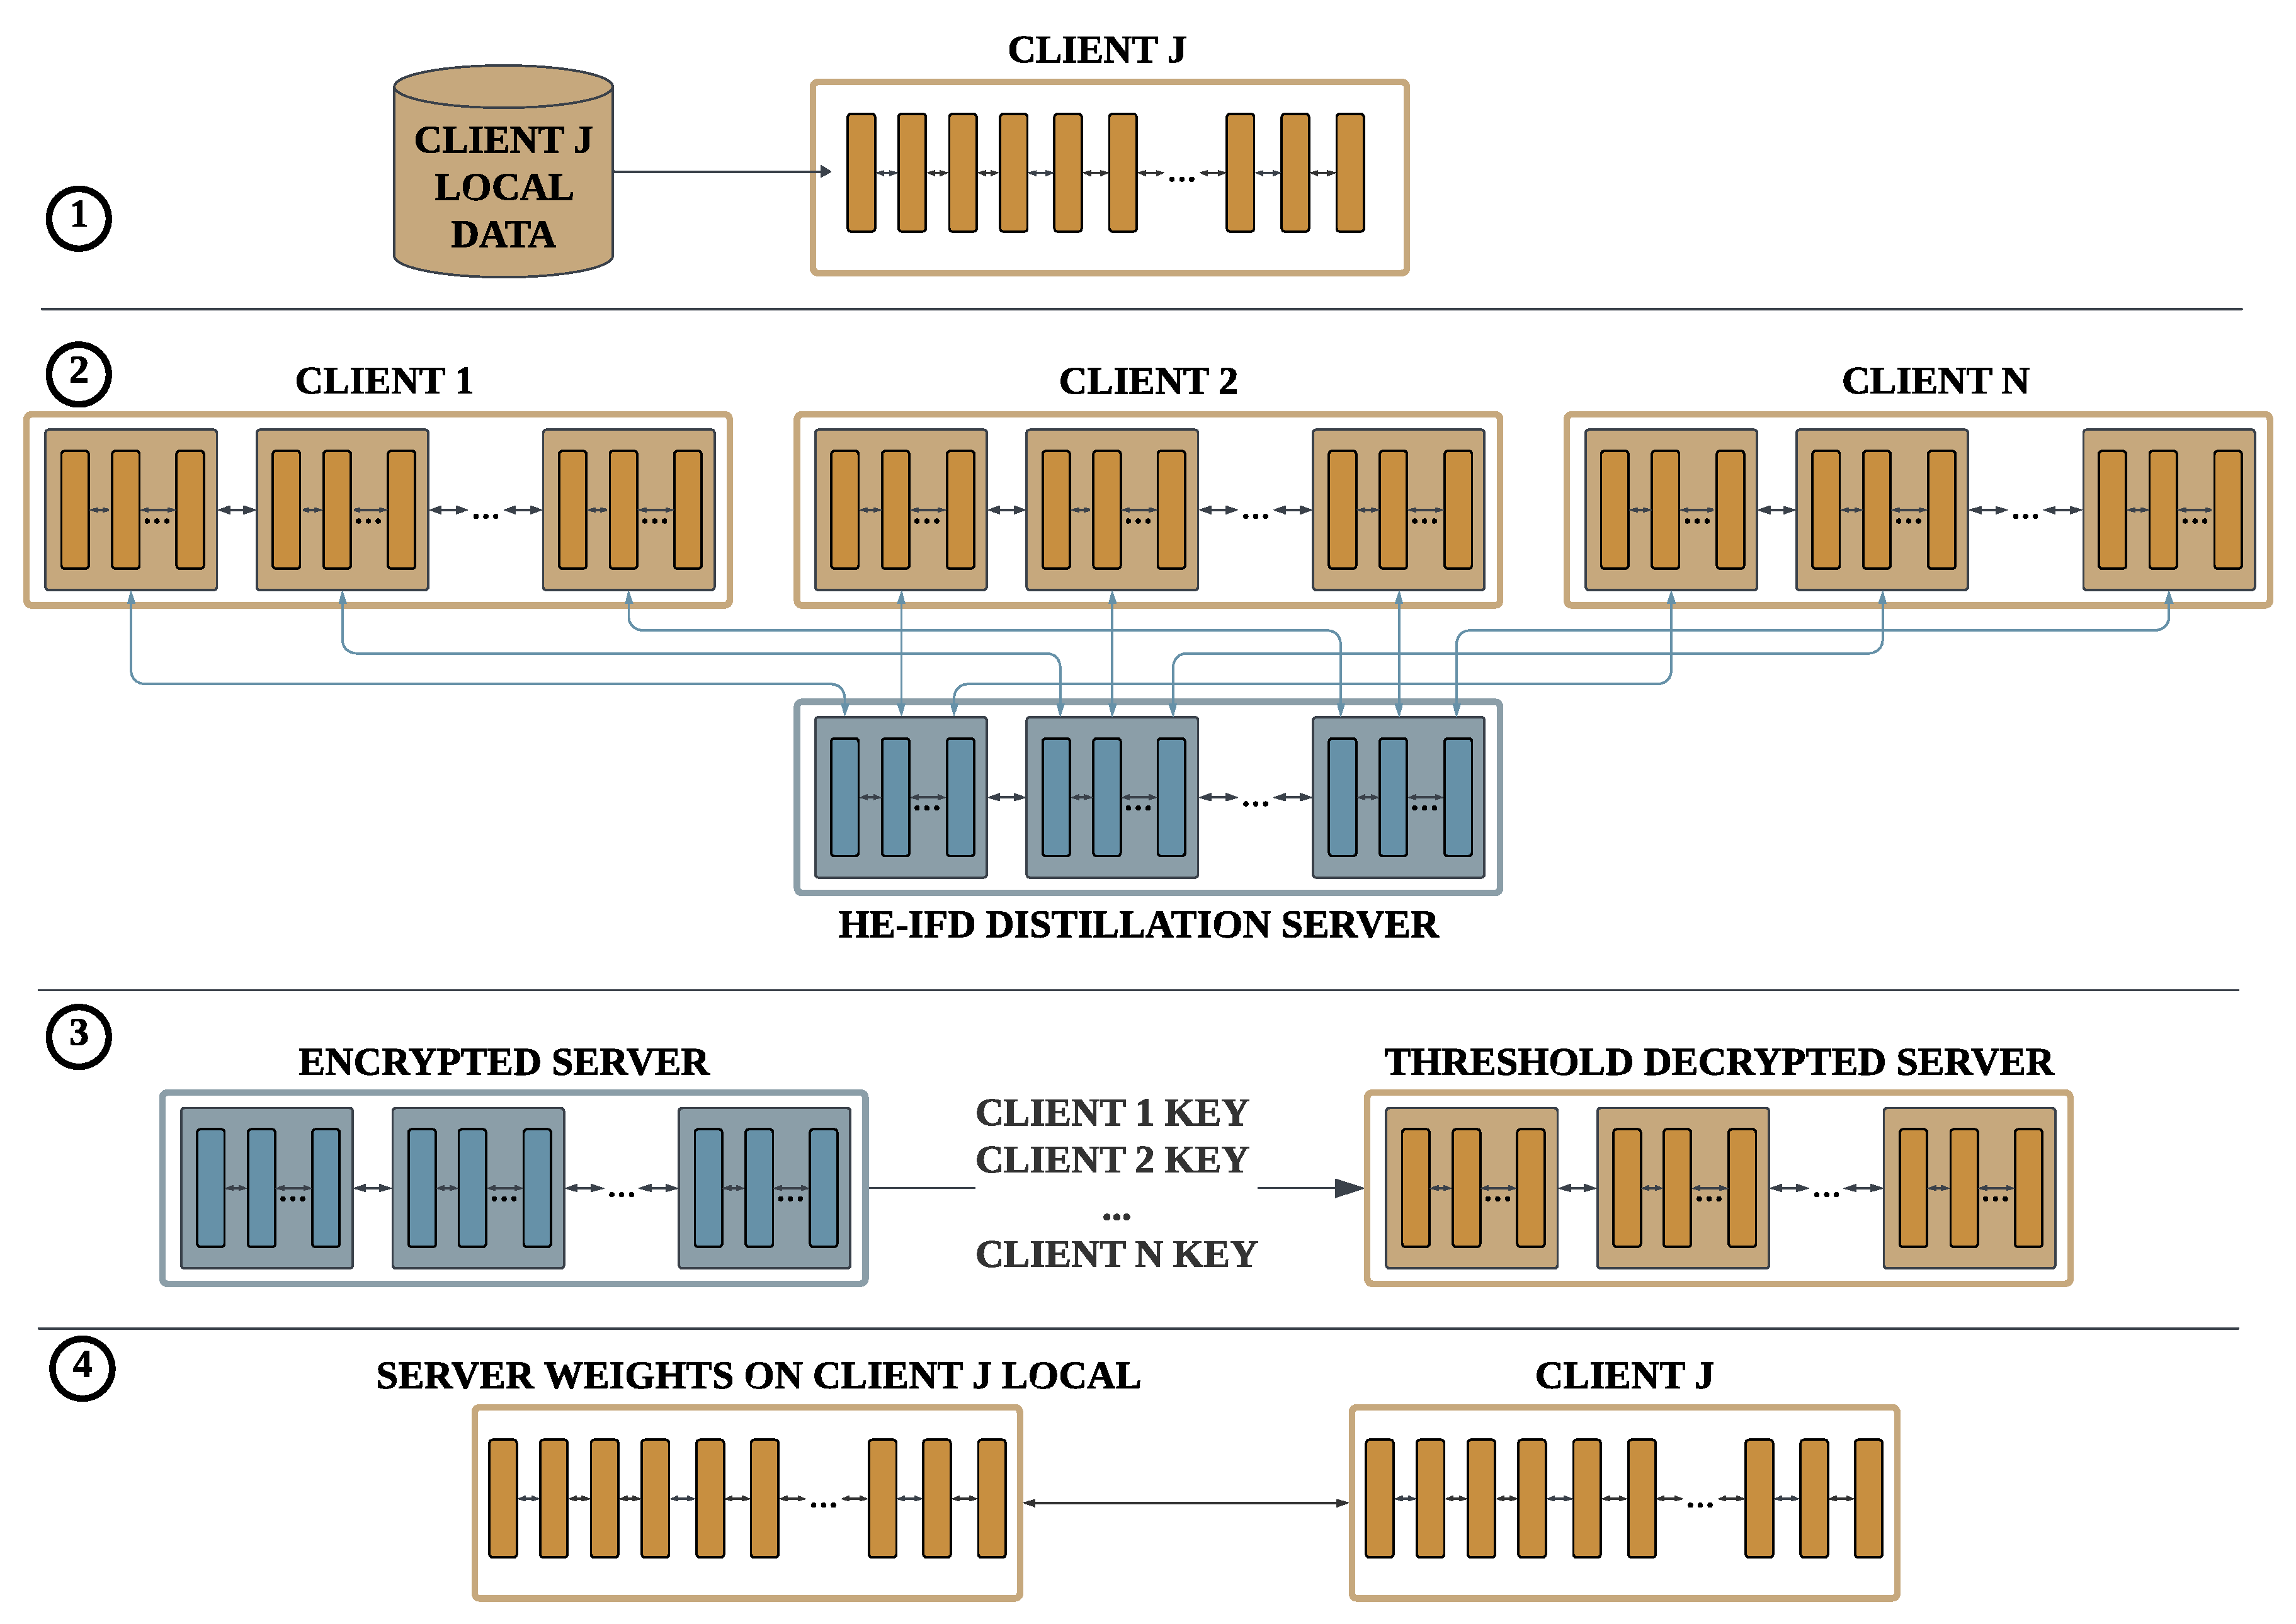
\includegraphics[width=0.87\textwidth]{figures/HE-IFD_sysFigure.pdf}
\caption{Overview of HE-IFD. \textcircled{1}~\textbf{Client-side training.} Each client independently trains a teacher model on its own private dataset. No data leaves the client device. \textcircled{2}~\textbf{Encrypted upload and server distillation.} Every client extracts intermediate feature representations at each block boundary of its teacher, normalises them per channel, encrypts them under the CKKS homomorphic encryption scheme, and uploads the ciphertexts to the server in a single communication round. The server pools encrypted features from all clients and trains a student model block by block, operating entirely on ciphertexts. The server never observes any plaintext data, weights, or intermediate values. \textcircled{3}~\textbf{Threshold decryption.} The server distributes the encrypted student model to all clients. Each client applies its secret key share locally to decrypt the model on its own device. No single client can decrypt alone, and the server never sees plaintext weights. \textcircled{4}~\textbf{Local model assembly.} Each client holds the decrypted student model in plaintext and may optionally fine-tune it on local data to adapt to its own distribution, with no further communication required.}
\label{fig:sys_figure}
\end{figure*}

\subsection{HE-IFD: One-Shot Distillation Framework}
\label{sec:framework}

This section presents the HE-IFD protocol in full generality. The framework applies to any architecture that admits a block decomposition with HE-compatible operations; architecture-specific instantiations are deferred to Section~\ref{sec:architecture}.

% \subsubsection{System Model and Threat Model}
% \label{sec:system_model}

\par\noindent\textbf{System Model.} We consider a cross-silo federated learning setting with $N$ clients and a central server. Each client $i$ holds a private dataset $\mathcal{D}_i$ that is never shared or transmitted. Clients wish to collaboratively train a shared student model by transferring knowledge from their locally trained teacher models to the server, without exposing their private data, including raw training data and any intermediate representations. Communication between clients and the server is restricted to a single round: each client sends a set of encrypted messages derived from its local data and model, after which the server performs all remaining computation independently with no further client interaction. An optional release phase at the end allows clients to collectively obtain the trained model.

\par\noindent\textbf{Threat Model.} We assume a semi-honest (honest-but-curious) server that follows the protocol faithfully but may attempt to infer private information from everything it observes. The adversary's goal is to infer information about a client's private dataset $\mathcal{D}_i$ or the client's local model, including individual samples, label distributions, or model weights, from the messages it receives during training. We further assume that the server may collude with up to $N-1$ clients; privacy of the remaining honest client's input is guaranteed by the threshold structure of the multiparty CKKS scheme described in Section~\ref{sec:phase3}, which requires the joint participation of all $N$ clients to decrypt any ciphertext.

Given this system and threat model, sending plaintext teacher outputs to the server is insufficient. Because, as discussed in Section~\ref{sec:bg_server_inference}, even a single round of plaintext knowledge transfer exposes clients to inference and inversion attacks. We therefore instantiate the knowledge transfer channel using the multiparty CKKS HE scheme~\cite{cheon2017ckks, mouchet2021multiparty} — the same construction implemented in Lattigo~\cite{lattigo} — which lets the server perform all distillation computation directly on ciphertexts under a public key whose corresponding secret key is held in shares across the $N$ clients.

% Under the IND-CPA security of CKKS, the server's entire view during training (encrypted feature pairs, intermediate activations, loss values, gradients, and student weights) is computationally indistinguishable from random. The server operates purely as a blind compute delegate and learns nothing about any client's private data. For additional protection, clients may add calibrated differential privacy noise before encryption, achieving $(\epsilon, \delta)$-differential privacy for the released model; this is optional since the cryptographic guarantee already prevents the server from inspecting any individual contribution during training.


% \subsubsection{Overview of HE-IFD}
% \label{sec:overview}

\par\noindent\textbf{Overview of HE-IFD.} HE-IFD proceeds in four phases, illustrated in Figure~\ref{fig:sys_figure} and formalised in Algorithm~\ref{alg:heifd}. In Phase~1, each client independently trains a teacher model on its private data. In Phase~2, clients extract intermediate features at each block boundary of the teacher, encrypt them under CKKS, and upload to the server in a single communication round, which is the only client-to-server interaction in the entire protocol. The server then trains an HE-compatible student model block by block on the pooled encrypted features. In Phase~3, clients collaboratively perform threshold decryption to obtain the trained student in plaintext. In Phase~4, each client receives the decrypted model (via joint threshold decryption) and may fine-tune it on local data to adapt to its own distribution.

The server never sees any plaintext data, model weights, or intermediate computations. All training happens on encrypted ciphertexts. Each block is trained independently with fresh ciphertexts, so multiplicative levels do not accumulate across blocks.


\begin{algorithm}[t!]
\small
\caption{HE-IFD: HE-Based Intermediate Feature Distillation}
\label{alg:heifd}
\begin{algorithmic}[1]
\REQUIRE $N$ clients with private datasets $\mathcal{D}_1, \ldots, \mathcal{D}_N$; student architecture $S$ with $K{+}1$ blocks
\ENSURE Trained student model $S$

\STATE \textbf{--- Phase 1: Client-Side Training (parallel, local) ---}
\FOR{each client $i = 1, \ldots, N$ \textbf{in parallel}}
    \STATE Train teacher $T_i$ on $\mathcal{D}_i$ via standard SGD
\ENDFOR

\STATE
\STATE \textbf{--- Phase 2: Encrypted Upload + Server Distillation ---}
\FOR{each client $i = 1, \ldots, N$ \textbf{in parallel}}
    \FOR{each block $k = 0, \ldots, K$}
        \STATE Extract feature pairs $(\mathbf{x}_k^{(i,j)}, \mathbf{y}_k^{(i,j)})$ by running $T_i$ on $\mathcal{D}_i$
        \STATE Normalise per channel: $\tilde{\mathbf{y}}_k \leftarrow (\mathbf{y}_k - \mu) / \sigma$ \hfill\COMMENT{Eq.~\ref{eq:client_norm}}
    \ENDFOR
    \STATE Encrypt all pairs under CKKS; upload $\{\enc{\mathbf{x}_k}, \enc{\tilde{\mathbf{y}}_k}\}$ to server \hfill\COMMENT{one-shot}
\ENDFOR

\STATE
\STATE \textit{Server-side (all computation on encrypted data):}
\STATE Initialise student $S$ with near-linear polynomial activations
\FOR{block $k = 0, \ldots, K$}
    \STATE Pool encrypted pairs from all $N$ clients for block $k$; shuffle
    \STATE Set depth-dependent hyperparameters: $\lambda_k, \eta_k$ \hfill\COMMENT{deeper blocks: stronger reg., lower LR}
    \FOR{epoch $= 1, \ldots, E$}
        \FOR{each mini-batch $(\enc{\mathbf{x}}, \enc{\tilde{\mathbf{y}}_k})$}
            \STATE $\hat{\mathbf{y}} \leftarrow S_{\text{block}[k]}(\enc{\mathbf{x}})$ \hfill\COMMENT{encrypted forward pass}
            \STATE $\mathcal{L} \leftarrow \mathcal{L}_{\text{MagReg}}(\hat{\mathbf{y}}, \enc{\tilde{\mathbf{y}}_k})$ \hfill\COMMENT{Eq.~\ref{eq:magreg}}
            \STATE Update $S_{\text{block}[k]}$ via encrypted gradient descent
        \ENDFOR
    \ENDFOR
    \STATE Freeze $S_{\text{block}[k]}$; initialise bridge $\mathbf{b}_k$ from feature statistics
\ENDFOR
\STATE Refine blocks sequentially with bridges on uploaded features ($R$ rounds)

\STATE
\STATE \textbf{--- Phase 3: Threshold Decryption ---}
\STATE All $N$ clients contribute key shares $\rightarrow$ decrypt $S$ to plaintext

\STATE
\STATE \textbf{--- Phase 4: Client-Side Model Assembly ---}
\FOR{each client $i = 1, \ldots, N$}
    \STATE Receive decrypted student $S$
    \STATE (Optional) Fine-tune $S$ on local data $\mathcal{D}_i$ with cross-entropy loss
\ENDFOR
\end{algorithmic}
\end{algorithm}

\subsubsection{Phase~1: Client-Side Training}
\label{sec:phase1}

Each client $i$ trains a teacher model $T_i$ on its private data $\mathcal{D}_i$ using standard supervised learning. All clients start from the same shared random weight initialisation. This phase is fully local, and no data leaves the client device.


\subsubsection{Phase~2: Encrypted Upload and Server-Side Distillation}
\label{sec:phase2}

Phase~2 has two parts: first, clients extract and upload encrypted features (one-shot); then, the server trains a student model entirely on these encrypted features.

\par\noindent\textbf{Feature extraction.} Each client runs its trained teacher on local data and extracts input-output feature pairs $(\mathbf{x}_k, \mathbf{y}_k)$ at every block boundary $k \in \{0, \ldots, K\}$, where block boundaries match the student architecture (Section~\ref{sec:architecture}). Clients use their own local data, not a shared auxiliary dataset. This is important: each teacher produces high-confidence outputs for the classes it has seen, and using local data preserves this specialisation rather than diluting it with uncertain predictions on unfamiliar classes.

\par\noindent\textbf{Normalisation.} Consistent normalisation across clients is essential for stable encrypted training. We adopt a collaborative normalisation approach where each client computes local statistics and the server aggregates them on encrypted data, following the privacy-preserving federated normalisation framework of~\cite{cosgun2025federated}. Before encryption, each client normalises features per channel to zero mean and unit variance:
\begin{equation}
    \mu_c^{(k,i)} = \mathbb{E}_{x \in \mathcal{D}_i}\!\left[ y_{k,c}(x) \right], \quad
    \sigma_c^{(k,i)} = \text{Std}_{x \in \mathcal{D}_i}\!\left[ y_{k,c}(x) \right]
    \label{eq:client_stats}
\end{equation}
\begin{equation}
    \tilde{y}_{k,c} = \frac{y_{k,c} - \mu_c^{(k,i)}}{\sigma_c^{(k,i)}}
    \label{eq:client_norm}
\end{equation}
where $y_{k,c}$ is the output of channel $c$ at block boundary $k$, $\mathbb{E}[\cdot]$ and $\text{Std}[\cdot]$ denote the mean and standard deviation over all samples in client $i$'s local dataset $\mathcal{D}_i$, and $C$ is the total number of channels at that block boundary. This is not optional since, without it, teachers trained on different distributions produce features with incompatible magnitude ranges, and the server's training diverges when pooling them.

\par\noindent\textbf{Encrypted upload.} Clients encrypt normalised features under CKKS and upload to the server. This is a single communication round and no further client interaction is needed. Normalisation statistics ($2C$ values per block per client, where $C$ is the number of channels)) may be sent in plaintext since they are aggregate quantities that reveal unimportant information about individual samples.


\par\noindent\textbf{Server-side distillation.} The server trains the student model block by block on the pooled encrypted features from all clients. For each block $k$, the server receives fresh encrypted input-output pairs $\left(\enc{\mathbf{x}_k^{(i,j)}},\, \enc{\tilde{\mathbf{y}}_k^{(i,j)}}\right)$ from every client $i$. It pools and shuffles them, then trains block $k$ via encrypted gradient descent. Upon convergence, block $k$ is frozen and the server moves to block $k{+}1$ using fresh ciphertexts.

This is the key design choice: each block trains on its own fresh ciphertexts, so CKKS multiplicative levels never accumulate across blocks. The total depth per block depends only on that block's structure, regardless of network depth.

Unlike federated averaging, the server does not aggregate teacher outputs. Each client's features provide independent gradient steps that accumulate into shared student weights. A client who specialises in certain classes contributes strong supervision for those classes, with no signal dilution.

\par\noindent\textbf{Train-inference distribution gap.} When block $k$ is trained on teacher features (ReLU-based: non-negative, sparse) but receives student features at inference (polynomial: signed, dense), a distribution gap arises. Empirically, composed accuracy collapses to ${\sim}10\%$ without addressing this.

We close this gap within the one-shot protocol by having each block trained in two stages. In the first stage, the block is trained on teacher features to learn the correct mapping. In the second stage (refinement), the block is fine-tuned on the uploaded encrypted data with a per-channel affine \textit{TrainableBridge} $\mathbf{b}_k(\mathbf{h}) = \boldsymbol{\gamma}_k \odot \mathbf{h} + \boldsymbol{\beta}_k$ that compensates for the distribution shift. Bridge parameters are initialised from feature statistics and co-trained with block weights during refinement.


\par\noindent\textbf{Loss Function.} Each block is trained with a magnitude-regularised normalised mean squared error loss. Student and teacher features are normalised per channel to zero mean and unit variance before computing the error:
\begin{equation}
    \mathcal{L}_{\text{NormMSE}} = \frac{1}{C} \sum_{c=1}^{C} \text{MSE}\!\left(\frac{\hat{f}_c - \mu_{\hat{f}_c}}{\sigma_{\hat{f}_c}},\; \frac{\tilde{f}_c - \mu_{\tilde{f}_c}}{\sigma_{\tilde{f}_c}}\right)
    \label{eq:normmse}
\end{equation}
where $\hat{f}_c$ and $\tilde{f}_c$ are the student prediction and normalised teacher target for channel $c$. This scale-invariant loss handles the distributional mismatch between student activations (signed, potentially large) and teacher activations.

\par\noindent\textbf{Magnitude regularisation.} The normalised loss alone is scale-invariant and permits the student to grow magnitudes without penalty. Since subsequent frozen polynomial blocks amplify any scale drift, we add a log-ratio penalty:
\begin{equation}
    \mathcal{L}_{\text{MagReg}} = \mathcal{L}_{\text{NormMSE}} + \lambda \cdot \frac{1}{C} \sum_{c=1}^{C} \left(\log \frac{\sigma_{\hat{f}_c}}{\sigma_{\tilde{f}_c}}\right)^{\!2}
    \label{eq:magreg}
\end{equation}
The log-ratio form is symmetric (penalising student magnitudes that are too large or too small equally) and scale-free (proportional to the multiplicative mismatch). The regularisation weight $\lambda$ scales with block depth: stronger regularisation is applied to deeper blocks where magnitude accumulation from the frozen chain is more severe.

\par\noindent\textbf{MSE on logits.} For the head block (block $K$), which outputs class logits, we use plain MSE without normalisation or magnitude regularisation, since logits are low-dimensional and do not exhibit the spatial channel structure of intermediate features. We use MSE rather than KL divergence because softmax is not a polynomial operation and cannot be evaluated under CKKS encryption. MSE on raw logits is HE-compatible because the squaring operation requires one ciphertext-ciphertext multiplication, and the remaining subtraction and averaging are level-free.


\subsubsection{Phase~3: Threshold Decryption}
\label{sec:phase3}

We instantiate the encrypted channel of HE-IFD with the multiparty CKKS protocol of~\cite{mouchet2021multiparty}, available in the open-source Lattigo library~\cite{lattigo}. We describe how the protocol is used in HE-IFD; the underlying construction is unchanged from the cited references and we treat it as a black box.

\par\noindent\textbf{Setup (before Phase~1).} The $N$ clients run a distributed key generation (DKG) protocol with no trusted dealer. Each client $i$ samples a secret-key share $\mathsf{sk}_i$ from the CKKS secret-key distribution and contributes a corresponding share to the protocol. The DKG output is (i)~a collective public key $\mathsf{pk}$ usable by everyone for encryption, (ii)~collective evaluation and rotation keys usable by the server for homomorphic computation, and (iii)~the secret-key shares $\{\mathsf{sk}_i\}_{i=1}^{N}$, kept privately by the clients. The full secret key $\mathsf{sk} = \sum_{i=1}^{N} \mathsf{sk}_i$ is never assembled at any single party at any point in the protocol.

\par\noindent\textbf{Encryption (Phase~2).} Every client encrypts its normalised feature pairs (Section~\ref{sec:phase2}) under the collective public key $\mathsf{pk}$ and uploads the ciphertexts to the server. From the server's perspective, the resulting ciphertexts behave exactly as ordinary single-key CKKS ciphertexts: the server applies homomorphic additions, ciphertext-by-plaintext multiplications, ciphertext-by-ciphertext multiplications (using the collective relinearisation key), and slot rotations (using the collective rotation keys) in the usual way. No client interaction is required during this phase.

\par\noindent\textbf{Collective decryption (Phase~3).} To release the trained student in plaintext, the server initiates a single round of \emph{collective key-switching}~\cite{mouchet2021multiparty}: it broadcasts the encrypted student weights $\enc{\mathbf{W}}$ to the clients, and each client $i$ contributes a key-switching share that re-encrypts $\enc{\mathbf{W}}$ from the collective key $\mathsf{pk}$ to a target key $\mathsf{pk}'$ (e.g., the all-zero key, which yields plaintext, or a fresh public key whose corresponding secret is held by a designated recipient). Every client's share is computed locally from $\mathsf{sk}_i$ and added a small smudging noise to mask its individual contribution. Combining all $N$ shares yields the re-encrypted ciphertext, from which $\mathbf{W}$ can be decrypted; combining any strict subset of $N-1$ shares yields a uniformly random ring element under the RLWE assumption~\cite{lyubashevsky2010ideal}. If this phase is skipped, the student stays encrypted and the server can serve encrypted inference directly.

\par\noindent\textbf{Trust assumption.} Privacy of every client's input holds as long as at least one of the $N$ clients is honest. This is strictly stronger than the trust assumption of single-key CKKS deployments, which require a trusted decryption authority, and matches the threat model of Section~\ref{sec:framework}: even if the server colludes with $N-1$ clients, the joint view consists of ciphertexts under a key whose remaining share is held by the honest client and is therefore computationally indistinguishable from random.


\subsubsection{Phase~4: Client-Side Model Assembly and Fine-Tuning}
\label{sec:phase4}

After local decryption, each client holds a copy of the trained student model in plaintext. Clients may fine-tune this model on their own private data using standard cross-entropy loss. This step requires no further communication with the server or other clients. Fine-tuning is particularly useful under non-IID settings, where the global student may underperform on a client's local distribution. We evaluate the accuracy impact of local fine-tuning in Section~\ref{sec:experiments}.


% \subsubsection{Algorithm}
% \label{sec:algorithm}


\subsection{Training Stability}
\label{sec:stability}

As established in Section~\ref{sec:introduction}, the composition of degree-$d$ polynomial activations across $L$ blocks yields an end-to-end map of degree $d^L$, whose magnitude bound grows doubly-exponentially in depth. This is a property of the function class rather than of any particular implementation, and it must be controlled by a combination of mechanisms that act on different parts of the protocol. Concretely:

\begin{itemize}[leftmargin=*,nosep]
    \item \textbf{Client-side normalisation} (Eq.~\ref{eq:client_norm}): ensures features from different clients have compatible magnitude ranges.
    \item \textbf{Magnitude-regularised loss} (Eq.~\ref{eq:magreg}): penalises scale drift between student and teacher outputs.
    \item \textbf{Gradient clipping}: prevents large updates from the quadratic term.
    \item \textbf{Depth-dependent hyperparameters}: deeper blocks use stronger regularisation and lower learning rates.
    \item \textbf{Per-channel affine bridges}: compensate for the absence of batch normalisation at block boundaries.
\end{itemize}

Section~\ref{sec:experiments} provides an ablation study quantifying the impact of each mechanism.


%% ================================================================
\subsection{Privacy Analysis}
\label{sec:privacy_proof}

%We provide a formal privacy argument for the HE-IFD protocol. 
%We assume the server is honest-but-curious: it follows the protocol but may try to learn client data from what it sees. We assume all $N$ clients are honest. 
During Phase~2, the server sees only CKKS-encrypted data: teacher block-boundary feature pairs, basic metadata such as tensor shapes and client count, and optional plaintext per-channel normalisation statistics. Raw client data and teacher model weights never leave the client. All server-side computations, i.e., forward passes, loss evaluation, gradient descent, and weight updates, are performed homomorphically on ciphertexts; student weights, intermediate activations, gradients, and loss values remain encrypted throughout Phase~2.

Under the Ring Learning with Errors (RLWE) assumption (with security parameter $\lambda \geq 128$), our protocol guarantees that the server learns no private information about individual client data during training. This relies on the IND-CPA security of the CKKS scheme~\cite{cheon2017ckks}, which means encrypted data cannot be distinguished from random noise. Because all homomorphic operations simply map ciphertexts to other ciphertexts, every intermediate calculation stays secure. As a result, the server's entire view of the training process can be simulated using only public parameters and metadata, proving no data is leaked. If clients choose to send their normalisation statistics in plaintext, these are aggregate quantities computed over the full local dataset and carry negligible information about any individual sample. For maximum security, these statistics can also be encrypted following the protocols in~\cite{cosgun2025federated}.

% If clients choose to decrypt the trained model for release, the resulting plaintext model has the same risk of membership inference attacks~\cite{shokri2017membership, carlini2022membership} as any standard machine learning model. Homomorphic encryption prevents data leakage during training without adding noise or limiting the number of training steps. In contrast, differential privacy adds noise to protect the final model, which lowers accuracy and limits how much training can be done. However, our protocol easily supports both: clients can add differential privacy noise to their data before encrypting it. This provides a formal $(\epsilon, \delta)$-differential privacy guarantee for the final decrypted model without changing how the encrypted training works.


%% ================================================================
\subsection{Architecture-Specific Instantiations}
\label{sec:architecture}

The HE-IFD framework described in Section~\ref{sec:framework} applies to any neural network that can be decomposed into blocks with HE-compatible operations. This section describes how we instantiate the framework for convolutional networks and vision transformers. The same principles extend to language models, which we discuss briefly for completeness.


\subsubsection{Convolutional Networks}
\label{sec:arch_cnn}

\par\noindent\textbf{PolyResNet-18.} The primary convolutional instantiation is PolyResNet-18, which is structurally identical to the ResNet-18 teacher but with all HE-incompatible operations replaced. This structural correspondence enables block-level feature matching between teacher and student. We summarize the replacements below: 

\par\noindent\textbf{ReLU $\to$ PolyAct.} ReLU ($\max(0, x)$) has no efficient polynomial representation under CKKS. We replace it with a learnable degree-2 polynomial:
\begin{equation}
    \text{PolyAct}(x) = ax^2 + bx + c
    \label{eq:polyact}
\end{equation}
initialised at $a = 0.3$, $b = 0.7$, $c = 0$, so that for normalised inputs the activation behaves approximately linearly, avoiding early magnitude divergence from the quadratic term. This near-linear initialisation strategy is consistent with prior work on stable polynomial-activation training~\cite{baruch2022methodology, garimella2021sisyphus}. The coefficients are learnable and adapt during training; after training, they are frozen as plaintext constants. Under CKKS, $x^2$ is one ciphertext-ciphertext multiplication (1 multiplicative level). The remaining terms ($ax^2, bx, c$) involve only plaintext-ciphertext operations (0 levels). Thus, the total cost is 1 multiplicative level per activation.

\par\noindent\textbf{BatchNorm $\to$ ChannelScale.} Batch normalisation computes a normalised output $\hat{x} = (x - \mu)/\sigma$ followed by a learnable affine transform. Under CKKS, the division $x/\sigma$ has no direct equivalent and must be approximated via iterative methods such as Goldschmidt's algorithm, which requires approximately 10 multiplicative levels per invocation. Since batch statistics are fixed after training, the normalisation can be folded into the affine parameters, leaving only the learnable scale and bias. We therefore replace BatchNorm with ChannelScale:
\begin{equation}
    \text{ChannelScale}(x) = \gamma \odot x + \beta
    \label{eq:channelscale}
\end{equation}
with learnable $\gamma$ (initialised to 1) and $\beta$ (initialised to 0). Since both are known plaintext at inference, this costs 0 multiplicative levels.

\par\noindent\textbf{MaxPool $\to$ Identity.} Max pooling is a comparison operation that requires non-polynomial approximations with prohibitive multiplicative depth under CKKS. For CIFAR-10 (32$\times$32 input), the initial max pool in standard ResNet-18 is replaced by an identity operation. Spatial downsampling is handled by stride-2 convolutions in deeper layers.

\par\noindent\textbf{PolyBasicBlock.} Each PolyBasicBlock, the residual building block of PolyResNet-18, follows the dataflow:
\begin{equation}
    x \xrightarrow{\text{conv}_1} \xrightarrow{\text{CS}_1} \xrightarrow{\text{PolyAct}_1} \xrightarrow{\text{conv}_2} \xrightarrow{\text{CS}_2} \xrightarrow{+\,\text{identity}} \xrightarrow{\text{PolyAct}_2} y
\end{equation}
where CS denotes ChannelScale and $+\,\text{identity}$ is the residual addition. Convolutions, ChannelScale, and the residual addition do not consume any levels. The two PolyAct invocations consume 1 level each, for a total of 2 multiplicative levels per block.

\par\noindent\textbf{Block boundaries.} We define six blocks for ResNet-18: Block~0 (stem) takes raw images as input and outputs the result after the first convolution, ChannelScale, and PolyAct. Blocks~1 through~4 correspond to the four residual layer groups, each containing two PolyBasicBlocks. Block~5 (head) processes the final layer's output into class logits via average pooling and a fully connected layer.

\par\noindent\textbf{Compact variants and simpler architectures.} We also evaluate PolyResNet-10 (one block per layer instead of two, approximately 5.6 million parameters) and PolyResNet-8 (three layers instead of four, approximately 1.5 million parameters) to study the effect of model capacity. For lightweight settings, we instantiate HEStudentCNN, a plain convolutional network with configurable channel widths, polynomial activations, and per-channel affine normalisation (no residual connections). These compact architectures demonstrate that the framework generalises beyond the ResNet family.


\subsubsection{Transformer and Vision Transformer Architectures}
\label{sec:arch_transformer}

HE-IFD naturally extends to transformer-based models through logit-level KL distillation rather than block-level feature matching. Transformer attention mechanisms create inter-layer dependencies that make intermediate feature matching less effective, but logit-level distillation requires only that the student match the teacher's final output distribution.

A key advantage of HE-IFD for transformers is its compatibility with pre-trained models. Rather than training from scratch, each client fine-tunes a pre-trained model (e.g., ViT-B/32 pre-trained on ImageNet) on their local data in Phase 1. This makes the framework practical for large models that would be infeasible to train from scratch on small client datasets. After encrypted distillation (Phase 2) and threshold decryption (Phase 3), clients receive the student model and may further fine-tune it locally in Phase 4 using standard (non-polynomial) activations, recovering any accuracy lost from HE-compatible replacements.

\par\noindent\textbf{Vision Transformer (ViT).} In Phase 1, each client takes a ViT-B/32 model pre-trained on ImageNet-1K (88M parameters) and fine-tunes it on their local private data partition to produce a teacher. In Phase 2, clients extract logits from their fine-tuned teachers, encrypt them, and upload to the server. The server distils these into an HE-compatible student where GELU activations are replaced with PolyGELU (degree-4 polynomial) and LayerNorm with AffineNorm. We evaluate on CIFAR-10 and FashionMNIST.


% \par\noindent\textbf{Language models (future work).} The same logit-level distillation extends to language models such as GPT-2 and DistilBERT by fine-tuning pre-trained models on client data partitions. Our preliminary experiments show that stable polynomial training for deep language models remains challenging, and we leave a full evaluation to future work.

\par\noindent\textbf{HE-compatible replacements for transformers.} Two operations in standard transformers are incompatible with CKKS: the GELU activation function and LayerNorm. We replace GELU with a degree-4 polynomial approximation (PolyGELU) fitted to match GELU over the range $[-5, 5]$. LayerNorm, which requires a division by the standard deviation, is replaced by AffineNorm: a per-element learnable scale and bias without any running statistics or normalisation division. These replacements are analogous to the PolyAct and ChannelScale substitutions in the convolutional setting.

\par\noindent\textbf{HE compliant student training.} To ease optimisation, we train transformer students in two phases. In the warmup phase, the student retains the standard GELU and LayerNorm activations, and is trained with KL divergence loss for several epochs to converge to a good parameter region. In the conversion phase, all GELU activations are replaced with PolyGELU and all LayerNorm layers are replaced with AffineNorm, and training continues with a reduced learning rate to adapt to the polynomial activation landscape. This two-phase strategy avoids the difficulty of training with polynomial activations from scratch, which we found to be unstable for transformer architectures.

\par\noindent\textbf{Memory efficiency.} For models with large output spaces, teacher logit tensors can be very large. We store averaged logits in half precision (float16), which halves memory usage with negligible impact on distillation quality. Logit averaging across clients is performed via in-place accumulation rather than stacking, reducing peak memory from three times the logit tensor size to two times.


%% ================================================================
\subsection{Communication and Computation Complexity}
\label{sec:complexity}

\subsubsection{CKKS Multiplication Budget}
\label{sec:ckks_budget}

Each ciphertext-ciphertext (CT$\times$CT) multiplication consumes one multiplicative level. Ciphertext-plaintext (CT$\times$PT) multiplications and all additions are level-free. Once a ciphertext's levels are exhausted, bootstrapping can refresh them, but at high computational cost.

On the server, \textbf{both the student weights and the client features are encrypted ciphertexts}. The server never holds plaintext weights or data. Every learnable operation (convolution, affine scaling, fully connected layers) is CT$\times$CT and consumes 1 level. Polynomial activations of degree $d$ consume $\lceil \log_2 d \rceil$ levels (e.g., degree-2 costs 1 level for $x^2$, degree-4 costs 2 levels for $x^2 \to x^4$). Additions (residual connections, bias terms) and plaintext-scalar operations (average pooling) are level-free, consuming no multiplicative depth.

\par\noindent\textbf{Per-block training depth.} HE-IFD trains each block independently with fresh ciphertexts, so levels never accumulate across blocks during Phase 2a. The depth consumed per block depends only on that block's internal structure. For the architectures we evaluate, a single block's forward pass consumes 4--16 levels depending on complexity. Adding loss computation (1 level for MSE) and the backward pass, the total per-block training depth fits within the budget provided by ring dimension $\log \mathcal{N} = 15$ (${\sim}$18 levels at 128-bit security). Phase 2a therefore, requires no bootstrapping. The cascade refinement in Phase 2b composes multiple blocks and exceeds the per-block budget, requiring bootstrapping to refresh levels between blocks (Section~\ref{sec:comm_comp}).


\par\noindent\textbf{Post-decryption inference.} After threshold decryption (Phase~3), weights become plaintext. Since weights are now plaintext constants, learnable operations (convolution, affine scaling) become plaintext-by-ciphertext multiplications, which do not consume multiplicative levels. Only polynomial activations, which involve ciphertext-by-ciphertext squaring, still consume levels.


\subsubsection{Computational Cost}
\label{sec:comp_cost}

On the client side, the dominating cost is training the local teacher model, which is standard supervised learning and scales with the size of each client's dataset. Feature extraction requires a single forward pass through the trained teacher and is comparatively inexpensive.

On the server side, training proceeds block by block. For each block, the server performs encrypted gradient descent over pooled client data. The per-iteration cost is higher than plaintext training due to CKKS ciphertext operations, but the total number of iterations is modest because the block-level supervision signal is direct (input-output pairs rather than end-to-end labels). 
% Refinement operates on features already held by the server and incurs no additional communication cost.

\subsubsection{Communication Cost}
\label{sec:comm_cost}

HE-IFD requires only a single communication round from each client to the server. The upload consists of encrypted input-output feature pairs for each block, plus per-channel normalisation statistics.

The dominant cost comes from encrypting intermediate feature maps, whose dimensionality far exceeds the normalisation statistics ($2C$ scalars) and evaluation keys (uploaded once per client). The total per-client upload volume is:
\begin{equation}
    C_{\text{client}} = \sum_{k=0}^{K} \left\lceil \frac{D_k}{S} \right\rceil \times N_{\text{samples}} \times C_{\text{CT}}
    \label{eq:comm_cost}
\end{equation}
where $D_k$ is the feature dimensionality at block boundary $k$, $S$ is the number of CKKS slots per ciphertext, $N_{\text{samples}}$ is the number of samples each client uploads, and $C_{\text{CT}}$ is the size of one ciphertext.

As a concrete example, in the ResNet-18 instantiation, Block~1 (the first residual layer group) produces feature maps of shape $64 \times 32 \times 32 = 65{,}536$ elements per sample. With 4096 CKKS slots per ciphertext (at ring dimension $\log \mathcal{N} = 13$), a single sample requires 16 ciphertexts per block boundary. Using 10\% of a 5000-sample local dataset gives 500 samples per client, amounting to 8{,}000 ciphertexts for Block~1 alone. At approximately 0.6~MB per ciphertext, this gives roughly 4.8~GB per client per block.

For transformer architectures using logit-level distillation, the communication cost depends on the output dimensionality and the number of samples. For ViT-B/32 on CIFAR-10 (10 classes), each client uploads encrypted logits for 5000 samples, which is modest (${\sim}$0.2~MB). For language models with large vocabularies, the cost is higher: a model with 50,000 output tokens and 5000 sequences of length 128 would produce a logit tensor of ${\sim}$48~GB in float32 or ${\sim}$24~GB in float16. Since logit-level distillation uses only a single "block" (the full model output), this is the total per-client upload. Note that the communication cost for multi-round encrypted FL \cite{sav2021poseidon,zhang2020batchcrypt} would be orders of magnitude larger, as each of the hundreds of training rounds requires encrypting and uploading full model gradient updates from every client. Vanilla (unencrypted) FL avoids encryption overhead but provides no privacy protection. In both cases, the HE-IFD upload is performed once and requires no further interaction.

% \section{METHODOLOGY}
% \label{sec:methodology}

% \begin{figure*}[t]
% \centering
% 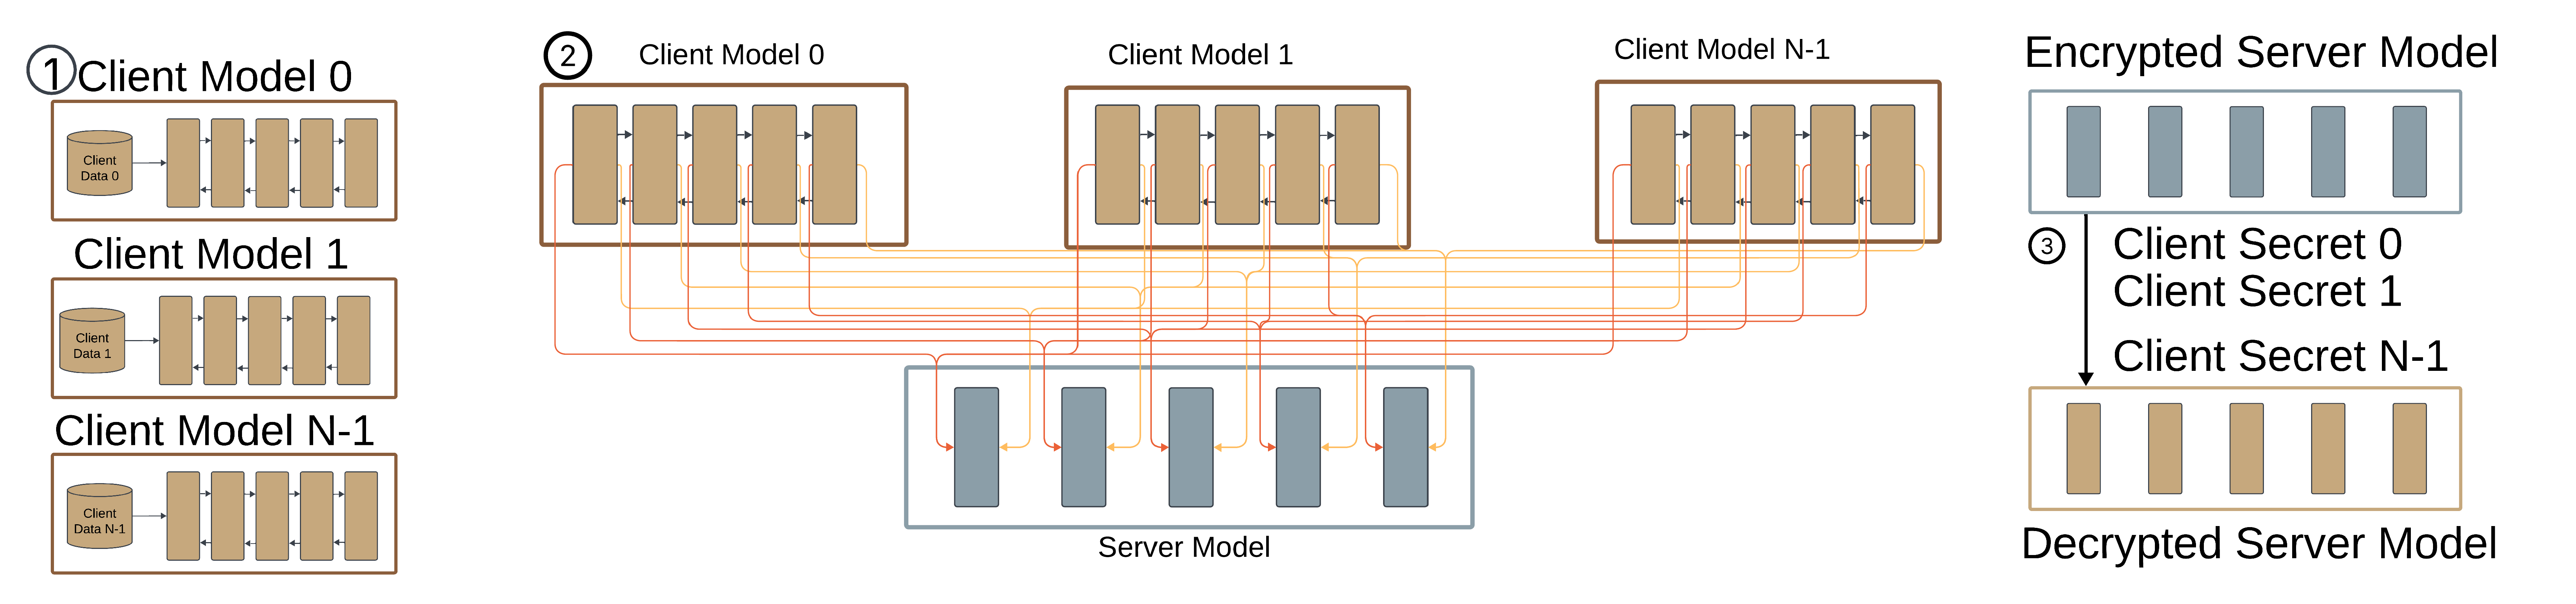
\includegraphics[width=\textwidth]{figures/SysFigureSimple.pdf}

% \caption{Overview of the HE-IFD framework. In Step~1 (Phase~1: Client-Side), each client independently trains a local teacher model on its private dataset, extracts per-block input--output feature pairs, normalises them collaboratively, and encrypts them under CKKS. In Step~2 (Phase~2: Server-Side Distillation), the server acts as a completely blind compute delegate, distilling these encrypted supervision signals block-by-block into an HE-compatible student model (e.g., PolyResNet-18) without ever observing plaintext data, weights, or activations. In Step~3 (Phase~3: Optional Model Release), clients collaboratively perform threshold decryption to release the trained model in plaintext.}

% \label{fig:sys_figure}
% \end{figure*}
 

% \subsection{System Model and Threat Model}
% \label{sec:system_model}

% \par\noindent\textbf{System Model.} We consider a cross-silo federated learning setting with $N$ clients and a central server. Each client $i$ holds a private dataset $\mathcal{D}_i$ that is never shared or transmitted. Clients wish to collaboratively train a shared student model by transferring knowledge from their locally trained teacher models to the server, without exposing their private data, including raw training data and any intermediate logits. Communication between clients and the server is restricted to a single round: each client sends a set of messages derived from its local data and model, after which the server performs all remaining computation independently with no further client interaction. An optional release phase at the end allows clients to collectively obtain the trained model.



% \par\noindent\textbf{Threat Model.} We assume a semi-honest (honest-but-curious) server that follows the protocol faithfully but may attempt to infer private information from everything it observes. All clients are assumed to behave honestly. The adversary's goal is to learn anything about a client's private dataset $\mathcal{D}_i$ or client's local model---including individual samples, label distributions, or model weights---from the messages it receives during training.


% Given this system and threat model, sending plaintext teacher outputs to the server is insufficient: as discussed in Section~\ref{sec:bg_server_inference}, even a single round of plaintext knowledge transfer exposes clients to inference and inversion attacks. We therefore instantiate the knowledge transfer channel using the CKKS homomorphic encryption scheme~\cite{cheon2017ckks}, which allows the server to perform all distillation computation directly on ciphertexts.


% Under the IND-CPA security of CKKS, the server's entire view during training, i.e., encrypted feature pairs, intermediate activations, loss values, gradients, and student weights, is computationally indistinguishable from random. The server operates purely as a blind compute delegate and learns nothing about any client's private data. For additional protection, clients may add calibrated differential privacy noise before encryption, achieving $(\epsilon, \delta)$-differential privacy for the released model; this is optional since the cryptographic guarantee already prevents the server from inspecting any individual contribution during training.



% % \subsubsection{CKKS Depth Budget and Protocol Phases}
% % \label{sec:encryption_params}

% % The CKKS scheme supports approximate arithmetic over real numbers but imposes a finite multiplicative depth budget: each ciphertext--ciphertext multiplication consumes one level, and once exhausted, the ciphertext can no longer be used. HE-IFD manages this budget by design.

% % \textbf{During training}, each block is trained independently with fresh ciphertexts. Since fresh ciphertexts start at full depth, there is no level accumulation across blocks regardless of network depth. The multiplicative depth consumed per block depends only on that block's internal structure: a single PolyBasicBlock containing two degree-2 polynomial activations consumes 2 levels in the forward pass, with additional levels for the backward pass chain rule through the polynomial terms.

% % \textbf{During encrypted inference} (post-deployment), the full student model requires 17 multiplicative levels for a complete forward pass (Section~\ref{sec:ckks_budget}), as the entire network is evaluated as a single encrypted circuit.

% % \textbf{At model release}, if clients elect threshold decryption, the student model weights are decrypted collaboratively and the model can subsequently be used for plaintext inference.


% % \textbf{At model release}, if clients elect threshold decryption, the student model weights are decrypted collaboratively and the model can subsequently be used for plaintext inference.

% \subsection{Overview of HE-IFD}
% \label{sec:overview}

% % Figure~\ref{fig:sys_figure} illustrates the three-phase HE-IFD protocol. In Step~1, each client independently trains a local teacher model on its private data and extracts intermediate feature pairs at each block boundary. In Step~2, clients normalise these features, encrypt them under CKKS, and upload the ciphertexts to the server in a single communication round, which is the only client--server interaction in the entire protocol. In Step~3, the server trains the HE-compatible student model block by block, operating entirely on ciphertexts without ever observing any plaintext data, weights, or activations. At model release, clients may collaboratively perform threshold decryption to obtain the trained student in plaintext; if omitted, the student remains encrypted and can be used directly for encrypted inference.

% HE-IFD proceeds in three phases, illustrated in Figure~\ref{fig:sys_figure} and formalised in Algorithm~\ref{alg:heifd}. In Phase~1, each client independently trains a local teacher model on its private data, extracts intermediate feature pairs at each block boundary, normalises them collaboratively, and uploads the encrypted ciphertexts to the server in a single communication round, which is the only client-to-server interaction in the entire protocol. In Phase~2, the server trains the HE-compatible student model block by block, operating entirely on ciphertexts. This phase proceeds in two stages: Phase~2a, in which each block is trained independently on encrypted teacher features; and Phase~2b, in which the server performs plaintext refinement using trainable bridges to close the train--inference distribution gap, requiring no additional client communication. In the optional Phase~3, clients collaboratively perform threshold decryption to obtain the trained student model in plaintext; if omitted, the student remains encrypted for direct encrypted inference.


% The phases are described in detail below.

% \subsubsection{Phase 1: Client-Side Local Training}
% \label{sec:phase1}

% Each client $i$ trains a local teacher model $T_i$ (e.g., ResNet-18) on their private data $\mathcal{D}_i$ using standard supervised learning. This phase is fully local, ensuring that no data or parameter leaves the client device.

% The server initialises common random weights $\theta_0$ to all clients before local training begins. Each client fine-tunes from $\theta_0$ on their private data. This is standard practice in federated learning and does not constitute a privacy violation: $\theta_0$ is randomly generated and carries no information about any client's data. 
% % In the next section we detail each step in client-side local training.

% % \textbf{Data partitioning.} Data is partitioned across clients using a Dirichlet distribution with concentration parameter $\alpha$, where $\alpha \to 0$ produces extreme non-IID partitions (each client sees few classes) and $\alpha \to \infty$ produces IID partitions. Our experiments evaluate $\alpha \in \{0.1, 0.5, 1.0, 100.0\}$ across $N \in \{1, 2, 4, 8, 16\}$ clients.

% \subsubsection{Phase 2: Per-Block Feature Extraction and Encrypted Upload}
% \label{sec:phase2}

% At a high level, after local training, each client extracts teacher representations at every block boundary, computes normalisation statistics, and uploads encrypted input-output pairs to the server.

% \par\noindent\textbf{Block Boundary Definitions.} We define six blocks matching the teacher and student architectures. Block 0 (stem) takes raw images as input and outputs the result post-conv1, batch normalisation, and ReLU. Block 1 (layer1) takes the stem output and yields features after two BasicBlocks. Blocks 2 through 4 correspond to layers 2 through 4, respectively, incorporating spatial downsampling. Finally, Block 5 (head) processes layer 4 outputs into class logits via average pooling and a fully-connected layer. For each defined block $k$, client $i$ extracts the tuple $(\textbf{x}_k, \textbf{y}_k)$, corresponding respectively to the block's input and output when running the teacher model on local data $\mathcal{D}_i$.

% \par\noindent\textbf{Local Data Protocol.} Each client generates teacher outputs on their \textit{own local training data}~$\mathcal{D}_i$, not on a shared auxiliary dataset. This design has two advantages. First, each teacher evaluates samples from its own training distribution, producing high-confidence supervision signals for the classes it has learned well. A client that specialises in a particular subset of classes provides strong logits and features for those classes, rather than uncertain outputs for classes it has not seen.
% Second, by using each client's data independently without aggregation, the signal from every individual client is preserved at full strength. Under the auxiliary-data protocol (evaluated as a comparison baseline in Section~\ref{sec:experiments}), averaging dilutes the useful signal from specialist clients with weak contributions from clients that have not seen the relevant classes.

% \par\noindent\textbf{Client-Side Collaborative Normalisation.} Before encryption, each client computes per-channel mean and standard deviation over their block-$k$ outputs. 
% For each channel $c$, they normalise their targets to zero mean and unit variance per channel before encryption:
% \begin{equation}
%     \mu_c^{(k,i)} = \mathbb{E}_{x \in \mathcal{D}_i}\!\left[ y_{k,c}(x) \right], \quad
%     \sigma_c^{(k,i)} = \text{Std}_{x \in \mathcal{D}_i}\!\left[ y_{k,c}(x) \right]
%     \label{eq:client_stats}
% \end{equation}
% \begin{equation}
%     \tilde{y}_{k,c} = \frac{y_{k,c} - \mu_c^{(k,i)}}{\sigma_c^{(k,i)}}
%     \label{eq:client_norm}
% \end{equation}
% where $\mu_c^{(k,i)}$ is the per-channel mean, $\sigma_c^{(k,i)}$ is the per-channel standard deviation, $y_{k,c}(x)$ is the $c$-th channel output of block $k$ for input $x$, and $\mathbb{E}$ and $\text{Std}$ denote expectation and standard deviation over the client's local dataset $\mathcal{D}_i$.



% This normalisation is a core component of the protocol, not an optional enhancement. Without it, teachers trained on different data distributions produce features with incompatible magnitude ranges. In our experiments, client-side normalisation eliminates NaN divergence that otherwise occurs at layer3 for $N \geq 4$ clients, and improves student accuracy from ${\sim}$19\% to ${\sim}$37\% at $N{=}4$, $\alpha{=}0.5$ (Section~\ref{sec:experiments}).

% The communication overhead is minimal: $2C$ floating-point values per block per client, where $C$ is the channel count. These statistics can be sent in plaintext (they are aggregate statistics over the client's data, not individual samples) or encrypted if stricter privacy is required.

%  \par\noindent\textbf{Communication Cost.} For each block $k$, client $i$ uploads encrypted input--output pairs for a subset of their local data. As a concrete example, Block~1 (layer1) produces feature maps of shape $64 \times 32 \times 32 = 65{,}536$ elements per sample. With 4096 CKKS slots per ciphertext, a single sample requires 16 ciphertexts per block boundary. Using 20\% of a 5000-sample local dataset (1000 samples), the per-client upload for Block~1 alone amounts to 16{,}000 ciphertexts, each approximately 0.6~MB at $\log N = 13$, giving roughly 9.6~GB per block. This motivates the data-efficiency discussion below.

% % Knowledge distillation is data-efficient: in our experiments, using 20--25\% of each client's local data provides sufficient supervision. The upload is one-shot---no further client interaction is needed during the server-side training loop.
% The upload is one-shot: no further client interaction is needed during the server-side training loop. In our experiments, each client contributes 10\% of their local data as encrypted supervision, which we find sufficient for stable distillation.


% % \subsubsection{Server-Side Block-Level Encrypted Distillation}
% % \label{sec:phase3}
% \subsubsection{Phase 2: Server-Side Distillation}
% \label{sec:phase2_server}

% The server trains the HE-compatible student model block by block. Each block is trained independently with its own fresh ciphertexts, and blocks are composed into the full model after all training is complete.

% \par\noindent\textbf{Block-Level Training.} For each block $k \in \{0, \ldots, 5\}$, the server receives fresh encrypted input--output pairs $\left(\enc{\mathbf{x}_k^{(i,j)}},\, \enc{\tilde{\mathbf{y}}_k^{(i,j)}}\right)$ sourced from every client $i$ and dataset sample $j \in \mathcal{D}_i$. The server conducts sequential multi-teacher training by pooling and shuffling all clients' pairs to bypass loss discontinuities. Gradient steps directly update the encrypted student weights for block $k$. Upon convergence, block $k$'s weights are frozen as permanent ciphertexts, allowing the server to advance to block $k{+}1$ using completely fresh ciphertexts.

% % \textit{No averaging, no aggregation:} Unlike federated averaging approaches, the server does not combine teacher outputs from different clients. Each client's data provides independent gradient steps that accumulate learning into the same set of student block weights. A client with high accuracy on birds contributes strong bird supervision; a client with high accuracy on trucks contributes strong truck supervision. The student learns from both without either signal being diluted.
% Unlike federated averaging approaches, the server does not combine teacher outputs from different clients. Each client's data provides independent gradient steps that accumulate learning into the same set of student block weights. A client with high accuracy on birds contributes strong bird supervision; a client with high accuracy on trucks contributes strong truck supervision. The student learns from both without either signal being diluted.


% % \textit{Fresh ciphertexts per block:} Each block starts training with fresh encrypted input--output pairs from the clients. This is the key design choice that avoids multiplicative level accumulation across blocks. Block $k$'s training consumes a fixed number of CKKS levels determined only by block $k$'s internal structure, regardless of how many blocks precede it.

% Each block starts training with fresh encrypted input--output pairs from the clients. This is the key design choice that avoids CKKS multiplicative budget accumulation across blocks. Block $k$'s training consumes a fixed number of CKKS budget determined only by block $k$'s internal structure, regardless of how many blocks precede it. By arranging the blocks carefully, we avoid costly bootstrapping operations completely.


% \par\noindent\textbf{Train--Inference Distribution Alignment.} For block $k > 0$, the input to block $k$ at inference is the output of the student's frozen prefix (blocks $0 \to k{-}1$). If block $k$ is instead trained on teacher-produced inputs, which we call \textit{teacher-input training}, a distribution gap arises: the features the teacher's prefix produces differ systematically from those the student's prefix produces, since the student uses polynomial activations rather than ReLU. If not addressed, this mismatch propagates through all subsequent blocks and causes the composed model to collapse toward random accuracy.

% % \textit{The ideal but communication-expensive fix.} The cleanest solution is \textit{student-input training}: after block $k{-}1$ is frozen, the server publishes its weights to all clients; each client runs the frozen student prefix locally and uploads fresh ciphertexts of the resulting student-produced inputs for block $k$. This completely eliminates the distribution gap but requires one additional client--server round per block---$K$ extra rounds for a $K$-block model---which conflicts with our one-shot communication objective.

% The cleanest solution is \textit{student-input training}: after block $k{-}1$ is frozen, the server publishes its weights to all clients; each client runs the frozen student prefix locally and uploads fresh ciphertexts of the resulting student-produced inputs for block $k$. This completely eliminates the distribution gap but requires one additional client--server round per block---$K$ extra rounds for a $K$-block model---which conflicts with our one-shot communication objective.


% Our approach is a one-shot upload with teacher-input and server-side alignment. We retain the one-shot upload property by using teacher-input training throughout Phase~2a but compensating for the distribution gap through two complementary mechanisms.

% % \textit{(i) Trainable bridges.} Each block group is followed by a \textit{TrainableBridge} module: a per-channel affine transform $\mathbf{b}_k(\mathbf{h}) = \boldsymbol{\gamma}_k \odot \mathbf{h} + \boldsymbol{\beta}_k$ with learned scale $\boldsymbol{\gamma}_k$ and bias $\boldsymbol{\beta}_k$. After Phase~2a, the server initialises each bridge to minimise the distribution shift from teacher-prefix to student-prefix features using the uploaded feature statistics:
% \par\noindent\textbf{Phase~2a: Encrypted Block-Level Training.} Each block group is followed by a \textit{TrainableBridge} module: a per-channel affine transform $\mathbf{b}_k(\mathbf{h}) = \boldsymbol{\gamma}_k \odot \mathbf{h} + \boldsymbol{\beta}_k$ with learned scale $\boldsymbol{\gamma}_k$ and bias $\boldsymbol{\beta}_k$. After Phase~2a, the server initialises each bridge to minimise the distribution shift from teacher-prefix to student-prefix features using the uploaded feature statistics:

% \begin{equation}
%     \boldsymbol{\gamma}_k \leftarrow \frac{\sigma\!\left[f^T_k(\mathbf{x})\right]}{\sigma\!\left[S_{0:k}(\mathbf{x})\right]}, \qquad
%     \boldsymbol{\beta}_k \leftarrow \mu\!\left[f^T_k(\mathbf{x})\right] - \boldsymbol{\gamma}_k \odot \mu\!\left[S_{0:k}(\mathbf{x})\right],
%     \label{eq:bridge_init}
% \end{equation}
% where $f^T_k$ denotes the teacher's block-$k$ output and $S_{0:k}$ the student chain through block $k$. This initialises each bridge as a near-identity transform (scale $\approx 1$, bias $\approx 0$) that aligns the student's feature distribution to the teacher's at each stage, preventing the cascade collapse that otherwise occurs in teacher-input training.

% % \textit{(ii) Server-side sequential refinement (Phase~2b).} After bridge initialisation, the server runs additional refinement rounds using the already-uploaded plaintext features. In each round, blocks are refined sequentially: block $k$ is trained on the actual output of the student's refined prefix (blocks $0 \to k{-}1$), with the teacher's block-$k$ output as the target. This is equivalent to student-input training, but executed entirely server-side on plaintext features---no additional client communication is required. Bridge parameters are co-trained alongside block weights during refinement.

% \par\noindent\textbf{Phase~2b: Server-Side Plaintext Refinement.} After bridge initialisation, the server runs additional refinement rounds using the already-uploaded plaintext features. In each round, blocks are refined sequentially: block $k$ is trained on the actual output of the student's refined prefix (blocks $0 \to k{-}1$), with the teacher's block-$k$ output as the target. This is equivalent to student-input training, but executed entirely server-side on plaintext features---no additional client communication is required. Bridge parameters are co-trained alongside block weights during refinement.

% The cryptographic cost analysis of both phases is provided in Section~\ref{sec:encryption_params}.



% \par\noindent\textbf{Loss Function.} Each block is trained with a magnitude-regularised normalised MSE loss.

% Student and teacher features are normalised per channel to zero mean and unit variance before computing MSE:
% \begin{equation}
%     \mathcal{L}_{\text{NormMSE}} = \frac{1}{C} \sum_{c=1}^{C} \text{MSE}\!\left(\frac{\hat{f}_c - \mu_{\hat{f}_c}}{\sigma_{\hat{f}_c}},\; \frac{\tilde{f}_c - \mu_{\tilde{f}_c}}{\sigma_{\tilde{f}_c}}\right)
%     \label{eq:normmse}
% \end{equation}
% where $\hat{f}_c$ and $\tilde{f}_c$ are the student prediction and normalised teacher target for channel $c$. This scale-invariant loss handles the distributional mismatch between PolyAct student activations (signed, potentially large) and ReLU teacher activations (non-negative, bounded).

% \par\noindent\textbf{Magnitude regularisation.} NormMSE alone is scale-invariant and permits the student to grow magnitudes without penalty. Since subsequent frozen polynomial blocks amplify any scale drift, we add a log-ratio penalty:
% \begin{equation}
%     \mathcal{L}_{\text{MagReg}} = \mathcal{L}_{\text{NormMSE}} + \lambda \cdot \frac{1}{C} \sum_{c=1}^{C} \left(\log \frac{\sigma_{\hat{f}_c}}{\sigma_{\tilde{f}_c}}\right)^{\!2}
%     \label{eq:magreg}
% \end{equation}
% The log-ratio form is symmetric (penalises student magnitudes that are too large or too small equally) and scale-free (proportional to the multiplicative mismatch). The regularisation weight $\lambda$ scales with block depth: $\lambda = 2$ for early blocks, increasing to $\lambda = 6$ for deeper blocks where magnitude accumulation from the frozen chain is more severe.

% \par\noindent\textbf{MSE on logits.} For the head block (block 5), which outputs class logits, we use plain MSE without normalisation or magnitude regularisation, since logits are low-dimensional and do not exhibit the spatial channel structure of intermediate features.

% We use MSE rather than KL divergence because softmax is not a polynomial operation and cannot be evaluated under CKKS encryption. MSE on raw logits is HE-compatible: the squaring operation requires one ciphertext--ciphertext multiplication (1 CKKS level), and the remaining subtraction and averaging are level-free.

% % \subsection{Protocol Summary}
% % \label{sec:algorithm}

% %     The HE-IFD protocol proceeds in three phases. In Phase~1 (local), each client independently trains a teacher model and extracts per-block input--output feature pairs from its private data. In Phase~2 (single upload), clients normalise their features using collaborative per-channel statistics, encrypt them under the CKKS scheme, and transmit the ciphertexts to the server in a single communication round. In Phase~3 (server-side distillation), the server trains the HE-compatible PolyResNet-18 student block by block, where each block receives fresh ciphertexts from all clients and is optimised via encrypted gradient descent before being frozen. An optional Phase~4 allows clients to collaboratively perform threshold decryption to release the trained model in plaintext. Algorithm~\ref{alg:heifd} formalises this procedure.


% % Before describing Phase~3, we summarise how HE-IFD manages the CKKS multiplicative depth budget across the protocol phases.

% \subsubsection{CKKS Depth Budget and Protocol Phases}
% \label{sec:encryption_params}

% The CKKS scheme supports approximate arithmetic over real numbers but imposes a finite multiplicative depth budget: each ciphertext--ciphertext multiplication consumes one level, and once exhausted, the ciphertext can no longer be used. HE-IFD manages this budget by design.

% \textbf{During training}, each block is trained independently with fresh ciphertexts. Since fresh ciphertexts start at full depth, there is no level accumulation across blocks regardless of network depth. The multiplicative depth consumed per block depends only on that block's internal structure: a single PolyBasicBlock (defined in Section~\ref{sec:polybasicblock}) containing two degree-2 polynomial activations consumes 2 levels in the forward pass, with additional levels for the backward pass chain rule through the polynomial terms.

% \textbf{During encrypted inference} (post-deployment), the full student model requires 17 multiplicative levels for a complete forward pass (Section~\ref{sec:ckks_budget}), as the entire network is evaluated as a single encrypted circuit.

% \textbf{At model release}, if clients elect threshold decryption, the student model weights are decrypted collaboratively and the model can subsequently be used for plaintext inference.

% \subsubsection{Phase~3 (Optional): Model Release}
% \label{sec:phase3}

% After server-side distillation is complete, the trained student model weights remain encrypted as ciphertexts on the server. Clients may collaboratively perform threshold decryption to obtain the student model in plaintext, after which it can be deployed for standard inference. If this phase is omitted, the student remains encrypted and can be used directly for encrypted inference without further client involvement.
% \par\noindent\textbf{CKKS depth constraint.} Teacher-input Phase~2a trains each block in isolation: block $k$ consumes only the CKKS levels determined by its own internal operations, independent of model depth. No level accumulation occurs across blocks, and no bootstrapping is needed during Phase~2a. Phase~2b refinement operates entirely on plaintext features already held by the server and therefore incurs no CKKS cost. At inference, the full student chain with bridges consumes levels sequentially; this depth budget is analysed in Section~\ref{sec:ckks_budget}.

% % \subsection{Details of HE-IFD}
% % \label{sec:details}
% % \hl{remove?}
% \begin{algorithm}[h!]
% \small
% \caption{HE-IFD: HE-Based Intermediate Feature Distillation}
% \label{alg:heifd}
% \begin{algorithmic}[1]
% \REQUIRE $N$ clients with private datasets $\mathcal{D}_1, \ldots, \mathcal{D}_N$; HE-compatible student architecture $S$ with $K{+}1$ blocks
% \ENSURE Trained student model $S$ (encrypted or decrypted)

% \STATE \textbf{--- Phase 1: Client-Side (parallel, local) ---}
% \FOR{each client $i = 1, \ldots, N$ \textbf{in parallel}}
%     \STATE Train teacher $T_i$ on $\mathcal{D}_i$ via standard SGD
%     \FOR{each block $k = 0, \ldots, K$}
%         \STATE Extract input--output pairs $(\mathbf{x}_k^{(i,j)}, \mathbf{y}_k^{(i,j)})$ by running $T_i$ on $\mathcal{D}_i$
%         \STATE Compute per-channel statistics: $\mu_c^{(k,i)}, \sigma_c^{(k,i)}$ over $\mathbf{y}_k$ \hfill\COMMENT{Eq.~\ref{eq:client_stats}}
%         \STATE Normalise targets: $\tilde{\mathbf{y}}_k^{(i,j)} \leftarrow (\mathbf{y}_k^{(i,j)} - \mu) / \sigma$ \hfill\COMMENT{Eq.~\ref{eq:client_norm}}
%     \ENDFOR
%     \STATE Encrypt all pairs under CKKS; upload $\{\enc{\mathbf{x}_k^{(i,j)}}, \enc{\tilde{\mathbf{y}}_k^{(i,j)}}\}$ to server
% \ENDFOR

% \STATE
% % \STATE \textbf{--- Phase 2: Server-Side Block Distillation ---}
% \STATE \textbf{--- Phase 2a: Server-Side Encrypted Distillation ---}

% \STATE Initialise student $S$ with near-linear PolyAct ($a{=}0.3, b{=}0.7, c{=}0$)
% \FOR{block $k = 0, \ldots, K$}
%     \STATE Pool encrypted pairs from all $N$ clients for block $k$; shuffle
%     \STATE Set $\lambda_k \leftarrow \lambda_{\text{base}} \cdot (1 + 2 \cdot k/K)$ \hfill\COMMENT{deeper blocks: stronger MagReg}
%     \STATE Set $\eta_k \leftarrow \eta_{\text{base}} \cdot (1 - 0.8 \cdot k/K)$ \hfill\COMMENT{deeper blocks: lower LR}
%     \FOR{epoch $= 1, \ldots, E$}
%         \FOR{each mini-batch $(\enc{\mathbf{x}}, \enc{\tilde{\mathbf{y}}_k})$}
%             \IF{$k = 0$}
%                 \STATE $\mathbf{h} \leftarrow \enc{\mathbf{x}}$ \hfill\COMMENT{raw image input}
%             \ELSE
%                 \STATE $\mathbf{h} \leftarrow \enc{\mathbf{x}_k}$ \hfill\COMMENT{teacher-produced input, uploaded by clients}
%             \ENDIF
%             \STATE $\hat{\mathbf{y}} \leftarrow S_{\text{block}[k]}(\mathbf{h})$ \hfill\COMMENT{current block forward}
%             \IF{$k < K$}
%                 \STATE $\mathcal{L} \leftarrow \mathcal{L}_{\text{NormMSE}}(\hat{\mathbf{y}}, \enc{\tilde{\mathbf{y}}_k}) + \lambda_k \cdot \mathcal{L}_{\text{MagReg}}(\hat{\mathbf{y}}, \enc{\tilde{\mathbf{y}}_k})$ \hfill\COMMENT{Eq.~\ref{eq:magreg}}
%             \ELSE
%                 \STATE $\mathcal{L} \leftarrow \text{MSE}(\hat{\mathbf{y}}, \enc{\tilde{\mathbf{y}}_k})$ \hfill\COMMENT{logit block}
%             \ENDIF
%             \STATE Update $S_{\text{block}[k]}$ via encrypted gradient descent with learning rate $\eta_k$
%         \ENDFOR
%     \ENDFOR
%     \STATE Freeze $S_{\text{block}[k]}$
% \ENDFOR

% \STATE
% \STATE \textbf{--- Phase 2b: Server-Side Plaintext Refinement ---}
% \STATE Initialise bridges; refine all blocks sequentially on uploaded plaintext features \hfill\COMMENT{Section~\ref{sec:phase2_server}}

% \STATE
% \STATE \textbf{--- Phase 3 (optional): Model Release ---}
% \STATE Clients collaboratively perform threshold decryption to obtain $S$ in plaintext
% \end{algorithmic}
% \end{algorithm}


% \subsection{HE-Compatible Student Architecture}
% \label{sec:architecture}

% The student is a PolyResNet-18 which is structurally identical to the teacher ResNet-18 but with all HE-incompatible operations replaced. This structural correspondence enables block-level feature matching between teacher and student.

% \subsubsection{Component Replacements}
% Here, we explain how we enable efficient execution of several functions in HE-IFD. 
% \par\noindent\textbf{ReLU $\to$ PolyAct.} ReLU is a function ($\max(0, x)$) with no efficient polynomial representation under CKKS. We replace it with a learnable degree-2 polynomial:
% \begin{equation}
%     \text{PolyAct}(x) = ax^2 + bx + c
%     \label{eq:polyact}
% \end{equation}
% % initialised at $a = 0.3$, $b = 0.7$, $c = 0$, so that the initial behaviour is approximately linear ($\text{PolyAct}(x) \approx 0.7x$ for small $x$). The coefficients are learnable and adapt during training; after training, they are frozen as plaintext constants. 

% initialised at $a = 0.3$, $b = 0.7$, $c = 0$, so that for normalised inputs ($|x| \leq 1$) the activation behaves approximately linearly ($\text{PolyAct}(x) \approx 0.7x$), avoiding early magnitude divergence from the quadratic term. This near-linear initialisation strategy is consistent with prior work on stable polynomial-activation training~\cite{baruch2022methodology, garimella2021sisyphus}; the specific values were validated empirically. The coefficients are learnable and adapt during training and after training, they are frozen as plaintext constants.


% Under CKKS, $x^2$ is one ciphertext--ciphertext multiplication (1 multiplicative level). The remaining terms ($ax^2, bx, c$) involve only plaintext--ciphertext operations (0 levels). Thus, the total cost is 1 multiplicative level per activation. 

% \par\noindent\textbf{BatchNorm $\to$ ChannelScale.} Batch normalisation computes a normalised output $\hat{x} = (x - \mu)/\sigma$ followed by a learnable affine transform. Under CKKS, the division $x/\sigma$ has no direct equivalent and must be approximated via iterative methods such as Goldschmidt's algorithm, which requires ${\sim}$10 multiplicative levels per invocation — far too expensive for a deep network. Since batch statistics are fixed after training, the normalisation can be folded into the affine parameters, leaving only the learnable scale and bias. We therefore replace BatchNorm with ChannelScale, a per-channel affine transform that is equivalent to BatchNorm at inference but costs zero multiplicative levels. 
% % We replace it with a per-channel affine transform:
% \begin{equation}
%     \text{ChannelScale}(x) = \gamma \odot x + \beta
%     \label{eq:channelscale}
% \end{equation}
% with learnable $\gamma$ (initialised to 1) and $\beta$ (initialised to 0). Since both are known plaintext at inference, this costs 0 multiplicative levels.

% \par\noindent\textbf{MaxPool $\to$ identity.} Max pooling is a comparison operation that requires non-polynomial approximations (e.g., iterative sign functions) with prohibitive multiplicative depth under CKKS. For CIFAR-10 (32$\times$32 input), the initial max pool in standard ResNet-18 was not adopted due to this high computational demand and is replaced by an identity operation. Spatial downsampling is handled by stride-2 convolutions in layers 2--4.

% \subsubsection{PolyBasicBlock Structure}\label{sec:polybasicblock}

% % Each PolyBasicBlockV2 follows the dataflow:
% Each PolyBasicBlock, the residual building block of PolyResNet-18, replacing the standard BasicBlock with HE-compatible operations, follows the dataflow:

% \begin{equation}
%     x \xrightarrow{\text{conv}_1} \xrightarrow{\text{CS}_1} \xrightarrow{\text{PolyAct}_1} \xrightarrow{\text{conv}_2} \xrightarrow{\text{CS}_2} \xrightarrow{+\,\text{identity}} \xrightarrow{\text{PolyAct}_2} y
% \end{equation}
% where conv denotes a convolution layer, CS denotes ChannelScale, PolyAct is the polynomial activation defined in Eq.~\ref{eq:polyact}, and $+\,\text{identity}$ is the residual addition.

% Convolutions, ChannelScale, and the residual addition consume 0 levels. The two PolyAct invocations consume 1 level each, for a total of 2 multiplicative levels per block.

% \subsubsection{Multiplicative Depth of CKKS Inference}
% \label{sec:ckks_budget}

% \begin{table}[h]
% \centering
% \caption{CKKS multiplicative levels for PolyResNet-18 encrypted inference}
% \label{tab:ckks_levels}
% \begin{tabular}{l|c|c|c}
% \hline
% \textbf{Component} & \textbf{Levels/Block} & \textbf{Blocks} & \textbf{Total} \\
% \hline
% Stem (conv $+$ CS $+$ PolyAct) & 1 & 1 & 1 \\
% Layer 1 (2 PolyBasicBlocks) & 2 & 2 & 4 \\
% Layer 2 & 2 & 2 & 4 \\
% Layer 3 & 2 & 2 & 4 \\
% Layer 4 & 2 & 2 & 4 \\
% AvgPool $+$ FC & 0 & --- & 0 \\
% \hline
% \textbf{Total} & & & \textbf{17} \\
% \hline
% \end{tabular}
% \end{table}

% % At inference, model weights are frozen plaintext constants. All operations involving weights (convolution, ChannelScale, FC) are plaintext--ciphertext and consume 0 levels. Only PolyAct's $x^2$ term consumes one multiplicative level per execution; all other operations are level-free.

% % During \textit{encrypted training}, server weights become ciphertext after the first gradient update involving encrypted targets. Operations previously marked PT$\times$CT become CT$\times$CT (1 additional level each). However, because each block trains independently with fresh ciphertexts, this increased cost is confined to the current block's depth budget and does not accumulate across the full network.

% \subsubsection{Total Number of CKKS Levels per Operation}

% Table~\ref{tab:he_ops} shows that at inference, only PolyAct consumes a multiplicative level (1 per invocation), since all other operations either involve plaintext weights (PT$\times$CT, 0 levels) or are level-free additions. During training, weights become ciphertext after the first gradient update, adding 1 level to convolution, ChannelScale, and the FC layer; however, since each block trains independently with fresh ciphertexts, this cost is confined to a single block and never accumulates across the network.

% \begin{table}[h]
% \centering
% \caption{CKKS costs per operation. At inference, weights are plaintext (PT) and activations are ciphertext (CT). During training, weights become CT after the first encrypted gradient update.}
% \label{tab:he_ops}
% \begin{tabular}{l|l|c|c}
% \hline
% \textbf{Operation} & \textbf{Inference} & \textbf{Inf.\ Levels} & \textbf{Train Levels} \\
% \hline
% Convolution & PT$\times$CT & 0 & 1 \\
% ChannelScale & PT$\times$CT & 0 & 1 \\
% PolyAct ($ax^2{+}bx{+}c$) & CT$\times$CT & 1 & 1 \\
% Residual add & CT$+$CT & 0 & 0 \\
% Average pooling & $\Sigma$CT $\times$ PT & 0 & 0 \\
% FC layer & PT$\times$CT & 0 & 1 \\
% \hline
% \end{tabular}
% \end{table}

% \subsection{Training Stability}
% \label{sec:stability}

% % Polynomial activations introduce unique training challenges that require multiple interlocking stability mechanisms.

% Polynomial activations introduce unique training challenges. We describe the main source of instability below and then present the interlocking mechanisms we deploy to address it.


% \subsubsection{Magnitude Accumulation}
% The quadratic term in PolyAct amplifies activation magnitudes at every composition. With $\text{PolyAct}(x) = 0.3x^2 + 0.7x$, an input of magnitude 5 produces output ${\sim}$11; a further composition gives ${\sim}$44. After 5 compositions (typical by layer3), magnitudes can reach $10^4$, causing NaN divergence. This problem is exacerbated under multi-client settings ($N \geq 4$), where heterogeneous client distributions increase feature variance through the frozen chain.

% The stability mechanisms described below address this problem directly.


% \subsubsection{Stability Mechanisms}

% % We deploy several interlocking mechanisms to counter instability. Client-side normalisation (Eq.~\ref{eq:client_norm}) bounds target ranges before encryption to avert cross-client magnitude mismatch. A magnitude-regularised loss (Eq.~\ref{eq:magreg}) constrains student scales to teacher targets, curtailing unbounded growth through frozen polynomial sequences. ChannelScale contributes per-channel affine capacity, substituting the variance normalisation lost by omitting batch normalisation. Strict gradient clipping ($\text{max\_norm} = 1.0$) inherently controls gradient explosion originating from quadratic terms. Crucially, student-input training (Section~\ref{sec:phase3}) subjects each block to the accurate inference-time distribution, precluding the catastrophic accuracy collapse characteristic of teacher-input paradigms. Furthermore, block-independent training employing fresh ciphertexts suppresses CKKS level accumulation, ensuring pristine numerical starts. Finally, deeper blocks incorporate strict learning rate scaling (operating down to $0.2\times$ base rates for layer 4) to mitigate sensitivity to accumulated perturbations from extended frozen prefix chains. 

% We deploy the following mechanisms to address the instability described above. Client-side normalisation (Eq.~\ref{eq:client_norm}) ensures that teacher features from different clients have compatible magnitude ranges before encryption. The magnitude-regularised loss (Eq.~\ref{eq:magreg}) penalises the student when its output scale drifts from the teacher target, preventing unbounded growth through the frozen polynomial chain. ChannelScale provides per-channel affine capacity at each block, compensating for the absence of batch normalisation. Gradient clipping (max\_norm$=$1.0) prevents large gradient steps from the quadratic term. Student-input training (Section~\ref{sec:phase2_server}) ensures each block is trained on the same input distribution it will receive at inference, avoiding the collapse observed in teacher-input training. Finally, learning rates are scaled down for deeper blocks (to $0.2\times$ the base rate at layer~4) to account for the larger input variance accumulated through the frozen prefix chain.


% Our ablation study (Section~\ref{sec:ablation}) quantifies the accuracy impact of removing each mechanism individually. In particular, removing client-side normalisation causes NaN divergence for $N \geq 4$; removing the magnitude regularisation penalty degrades accuracy by ${\sim}$18\%; and replacing student-input with teacher-input training reduces accuracy from ${\sim}$71\% to ${\sim}$12\%.

% \subsection{Privacy Analysis}
% \label{sec:privacy_proof}

% %We provide a formal privacy argument for the HE-IFD protocol. 
% We assume the server is "honest-but-curious": it follows the protocol but may try to learn client data from what it sees. We assume all $N$ clients are honest. During training, the server only sees CKKS-encrypted input--output pairs, basic metadata such as the number of clients and tensor sizes, and optional plaintext normalisation statistics. Everything else---such as student weights, activations, losses, and gradients---is computed homomorphically and remains fully encrypted.

% Under the Ring Learning with Errors (RLWE) assumption (with security parameter $\lambda \geq 128$), our protocol guarantees that the server learns no private information about individual client data during training. This relies on the IND-CPA security of the CKKS scheme~\cite{cheon2017ckks}, which means encrypted data cannot be distinguished from random noise. Because all homomorphic operations simply map ciphertexts to other ciphertexts, every intermediate calculation stays secure. As a result, the server's entire view of the training process can be simulated using only public parameters and metadata, proving no data is leaked. If clients choose to send their normalisation statistics in plaintext, these are aggregate quantities computed over the full local dataset and carry non-critical information about any individual sample. For maximum security, these statistics can also be encrypted. Thus, privacy against server is achieved.

% If clients choose to decrypt the trained model for release, the resulting plaintext model has the same risk of membership inference attacks by clients~\cite{shokri2017membership, carlini2022membership} as any standard machine learning model. Homomorphic encryption prevents data leakage during training without adding noise or limiting the number of training steps. In contrast, differential privacy (DP) adds noise to protect the final model, which lowers accuracy and limits how much training can be done. However, our protocol easily supports both: clients can add DP noise to their data before encrypting it. This provides a formal $(\epsilon, \delta)$-DP for the final decrypted model without changing how the encrypted training works.

\section{EXPERIMENTS}
\label{sec:experiments}

\subsection{Setup}
\label{sec:exp_setup}

We evaluate HE-IFD on two image classification datasets (CIFAR-10~\cite{krizhevsky2009learning} and FashionMNIST~\cite{xiao2017fashion}) with two model families (ResNet-18 and SimpleCNN), and extend the evaluation to pre-trained Vision Transformers (ViT-B/32). All accuracy experiments run as plaintext simulations of the encrypted protocol to expedite the evaluation: we execute the exact same forward and backward passes, loss functions, and weight updates that the CKKS-encrypted server would perform, and validate numerical equivalence against TenSEAL-based encrypted operations in Section~\ref{sec:ckks_validation}.

\textbf{Data partitioning.} Client data is split using a Dirichlet distribution with concentration parameter $\alpha$, where a smaller $\alpha$ produces more heterogeneous partitions. We use $\alpha \in \{0.1, 1.0\}$ (extremely heterogeneous and heterogeneous) across $N \in \{1, 2, 4, 8, 16, 32\}$ clients.

\textbf{ResNet-18.} Each client trains a ResNet-18 teacher (11.2M parameters) for 200 epochs. The server distils into a PolyResNet-18 student with polynomial activations and per-channel affine scaling. Phase 2 trains each block independently on encrypted teacher features (80 epochs per block), then refines the cascade sequentially with bootstrapping to close the train-inference distribution gap. Each client contributes only 5000 samples (10\% of CIFAR-10's 50,000 training images). This is a deliberate experiment choice, as intermediate feature distillation is data-efficient because teacher features provide direct per-block supervision, and the server trains on pooled features from all clients. Using a small fraction of each client's data keeps the upload volume manageable while achieving strong accuracy.

\textbf{SimpleCNN.} We train SimpleCNN teachers (0.3M parameters, 4 conv layers) and distil into an HE-compatible polynomial student. %The pattern matches ResNet-18 across all settings.

\textbf{Vision Transformer.} We fine-tune pre-trained ViT-B/32 (ImageNet-1K, 88M parameters) on CIFAR-10 and FashionMNIST, replacing GELU with PolyGELU (degree-4) and LayerNorm with AffineNorm. %Oracle reaches 92\% on CIFAR-10 and 91\% on FashionMNIST. The same degradation pattern holds.

\begin{figure}[t]
\centering

\includegraphics[width=0.45\textwidth]{figures/fig_main_resnet18.pdf}
\caption{HE-IFD accuracy on CIFAR-10 (top) and FashionMNIST (bottom) with ResNet-18 teachers and PolyResNet-18 student. The two plaintext reference lines are the centralised Oracle (dashed gray, upper bound trained on all pooled data with no privacy protection) and the mean individual teacher accuracy at each setting (solid gray, the natural local-only floor each client could achieve without collaboration). HE-IFD (orange) approaches the Oracle at small $N$ and consistently outperforms the mean teacher across all settings.}
\label{fig:main_resnet18}
\end{figure}

\textbf{Reference points.} We anchor every accuracy curve in this section to two plaintext references that bracket the achievable range without our protocol:
\begin{itemize}[nosep]
    \item \textbf{Oracle}: a standard ResNet-18 trained on all pooled data in plaintext, with no privacy protection. This is the centralised upper bound on accuracy and the strongest possible baseline a non-private system could achieve.
    \item \textbf{Mean individual teacher}: the unweighted average accuracy of the $N$ local teacher models, each evaluated on the global test set after being trained only on its own private partition. This is the strongest accuracy that any client could obtain on its own without collaboration, and it is the relevant comparator for assessing whether participating in the protocol is worthwhile.
\end{itemize}
We do not include a separate plaintext-KL distillation baseline: the question this paper addresses is not how polynomial activations compare with ReLU under standard distillation (a centralised question, already studied in~\cite{baruch2022methodology, agamennone2025polynomial, alhossain2025training}), but whether a one-shot encrypted federated protocol can recover an accuracy that lies between the local-only mean teacher and the centralised Oracle.

In the rest of this section, \textbf{HE-IFD} refers to our method. For ResNet-18 experiments the student is PolyResNet-18, for SimpleCNN experiments, the student is HEStudentCNN, and for ViT experiments, the student is a ViT-B/32 with GELU replaced by PolyGELU and LayerNorm replaced by AffineNorm (Section~\ref{sec:arch_transformer}).

\subsection{Accuracy Results}
\label{sec:main_results}

Figure~\ref{fig:main_resnet18} shows accuracy across all settings on CIFAR-10 and FashionMNIST datasets. We summarize the key takeaways below: 

\textbf{HE-IFD consistently exceeds the mean teacher.} Across all settings with $\alpha \leq 1.0$, the encrypted student outperforms the average individual teacher by 10--20 percentage points. The student aggregates complementary knowledge from heterogeneous specialists into a single model that no individual client could construct from its own data alone.

% \textbf{HE-IFD approaches Oracle-level performance at low $N$.} On CIFAR-10, HE-IFD reaches 79.2\% at $N{=}1$ and $\sim67\%$ at $N{=}2$ while Oracle achieves 78.5\%. On FashionMNIST, it reaches 89.9\% at $N{=}1$ and 87--88\% at $N{=}2$ and the Oracle achieves 90.0\%. The encrypted student achieves accuracy comparable to a centralised model trained on all data in plaintext. This shows that the effect of encryption on accuracy, when compared with the centralised model, remains unimportant.

\textbf{The effect of encryption remains negligible.} On CIFAR-10, HE-IFD reaches 79.2\% at $N{=}1$ while Oracle achieves 78.5\%. On FashionMNIST, it reaches 89.9\% at $N{=}1$, and the Oracle achieves 90.0\%. Thus, the encrypted student achieves accuracy comparable to a centralised model trained on all data in plaintext. This shows that the effect of encryption on accuracy, when compared with the centralised model, remains negligible. 
\begin{figure}[t]
\centering

\includegraphics[width=0.45\textwidth]{figures/fig_arch_gen.pdf}
\caption{Architecture generalisation on CIFAR-10. Top row: SimpleCNN for $N$ in {1,2,4,8,16,32}. Bottom row: pre-trained ViT-B/32 for $N$ in {1,4,16} (fewer values because fine-tuning the 88M-parameter ViT teacher is computationally expensive). Left column: alpha=0.1, right column: alpha=1.0. The same trend from ResNet-18 holds across architectures: HE-IFD (orange) follows a similar trend to the Oracle across all settings.}
\label{fig:arch_gen}
\end{figure}
\textbf{HE-IFD tracks the centralised Oracle as $N$ increases.} At $N{=}4$, $\alpha{=}0.1$, HE-IFD achieves 57\% on CIFAR-10 and 85\% on FashionMNIST. At $N{=}16$, $\alpha{=}0.1$, it reaches 35--37\% and 65--67\%, respectively. The Oracle, which has no privacy constraint and sees all pooled data, degrades along the same shape as the per-client partition shrinks; HE-IFD's curve runs roughly parallel to it across $N$. This confirms that the residual accuracy loss is attributable to data fragmentation across more clients (weaker individual teachers), not to the encryption.

% \subsection{Architecture Generalisation}
% \label{sec:arch_gen}

We also evaluate HE-IFD on SimpleCNN and pre-trained ViT-B/32 to confirm the framework generalises beyond ResNet. Figure~\ref{fig:arch_gen} shows results on both datasets for $\alpha \in \{0.1, 1.0\}$. We summarize our findings below: 

\textbf{SimpleCNN.} HE-IFD follows a similar trend to the Oracle at small $N$ and degrades with more clients, consistent with the ResNet-18 results.

\textbf{Vision Transformer.} Oracle fine-tuning reaches 92\% on CIFAR-10 and 91\% on FashionMNIST (shown as the dashed gray Oracle line in Figure~\ref{fig:arch_gen}). HE-IFD follows a similar trend, with accuracy closest to the Oracle at $N$=1 and declining at larger $N$. After threshold decryption (Phase 3), clients may further fine-tune the received model on local data using standard GELU and LayerNorm, improving accuracy on their local distributions.


\subsection{Privacy Analysis}
\label{sec:dp_comparison}

We compare HE-IFD against two differential privacy (DP) baselines on ResNet-18 CIFAR-10 at $N{=}4$, chosen so that the comparison spans both axes of the design space: the type of guarantee (statistical vs.\ cryptographic) and the number of communication rounds (one-shot vs.\ multi-round). Local Differential Privacy (LDP)~\cite{kasiviswanathan2011can} perturbs each client's data locally before upload and is therefore one-shot compatible; DP-SGD~\cite{abadi2016deep} injects calibrated Gaussian noise into per-sample gradients during multi-round training. Both yield a statistical $(\varepsilon, \delta)$-guarantee parameterised by the privacy budget $\varepsilon$, with smaller $\varepsilon$ corresponding to stronger privacy but more noise and lower utility. HE-IFD provides a cryptographic guarantee under the IND-CPA security of multiparty CKKS (Section~\ref{sec:phase3}): the server's view consists of ciphertexts under a key whose corresponding secret is held in shares across the clients, and any inference about the inputs of an honest client reduces to breaking RLWE. Among the three, HE-IFD is the only one-shot mechanism with a cryptographic guarantee. Figure~\ref{fig:privacy} shows the privacy-utility trade-off; HE-IFD appears as a single point at MIA AUC = 0.5 because the AUC is 0.5 by construction during training, independent of attack strength. Key findings:

\begin{figure}[t]
\centering
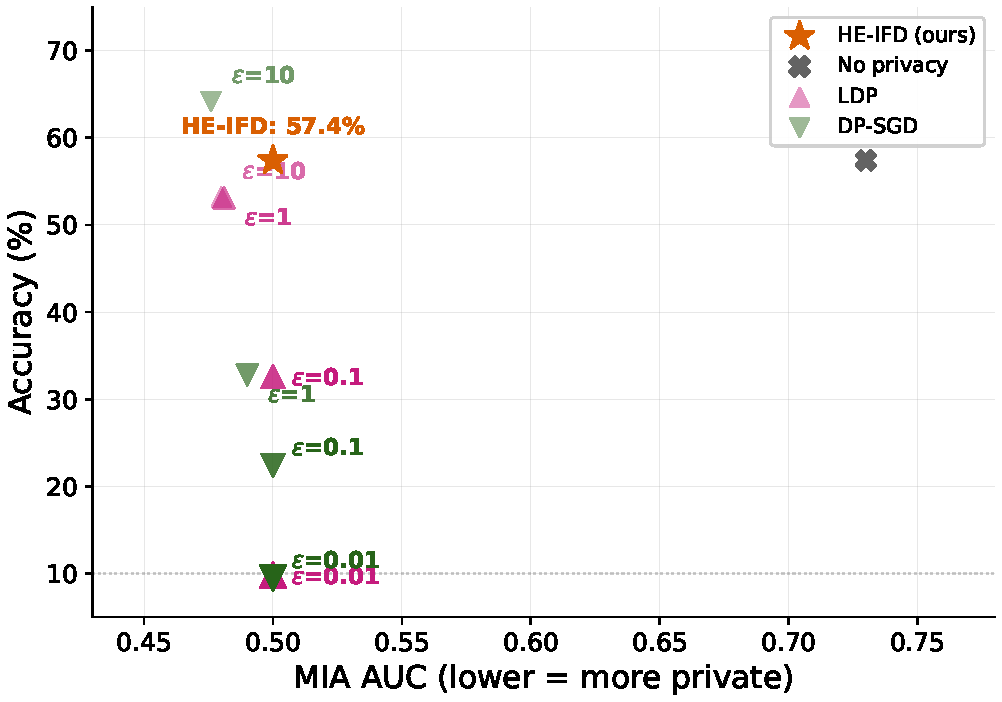
\includegraphics[width=0.45\textwidth]{figures/fig_privacy.pdf}
\caption{Privacy-utility trade-off for ResNet-18 on CIFAR-10 ($N{=}4$). HE-IFD (orange point) provides accuracy without an attack surface; by ensuring the server never sees plaintext, it makes membership inference impossible during training (MIA AUC=0.5). LDP and DP-SGD points are shown with $\varepsilon$ labels; darker markers indicate tighter privacy. At $\varepsilon{=}0.01$, both collapse to random-guess accuracy (${\sim}10\%$) while still providing only a statistical guarantee. HE-IFD achieves comparable or better accuracy with a strictly stronger, cryptographic guarantee.}
\label{fig:privacy}
\end{figure}

\textbf{HE-IFD matches the best DP-SGD accuracy with stronger privacy.} At $N{=}4$, $\alpha{=}0.1$, HE-IFD reaches 57.4\% while the best DP-SGD ($\varepsilon{=}10$, weakest privacy) reaches 64.2\%. At $\varepsilon{=}1$, DP-SGD drops to 33\%. At $\varepsilon{=}0.01$, training collapses to 10\%. HE-IFD achieves competitive accuracy without any noise injection and with a cryptographic rather than statistical privacy guarantee.

\textbf{Membership inference confirms the cryptographic advantage.} We evaluate LiRA~\cite{carlini2022membership} membership inference attacks with 8 shadow models, alongside loss-threshold~\cite{yeom2018privacy} and confidence-based~\cite{salem2019ml} attacks. Against the plaintext distillation student, LiRA achieves AUC 0.73, confirming high privacy risk from unencrypted logit transfers. HE-IFD eliminates this attack surface entirely: the server processes only ciphertexts, making membership inference computationally infeasible during training.

\textbf{Client-to-client privacy after model release.} After threshold decryption (Phase 3), each client holds the trained model in plaintext. At this point, standard membership inference risks apply to the released model, as with any machine learning model. However, the model was trained on pooled encrypted features from all $N$ clients, so each individual client's contribution is diluted across the full training set. LiRA applied by one client against another requires shadow models trained on overlapping data, which is not possible when each client holds only its own private partition. The practical client-to-client inference risk is therefore limited to what can be extracted from the released model's predictions, comparable to any published/deployed machine learning model.


% \subsection{Communication and Computation}
% \label{sec:comm_comp}

\subsection{Communication Cost}
\label{sec:comm_comp}

HE-IFD requires a single upload per client. Each client encrypts teacher feature pairs under CKKS and uploads them along with evaluation keys. Clients upload only 10\% of their local data, which is sufficient for high-accuracy distillation because intermediate features provide direct per-block supervision. This upload happens once, and no further client-server interaction occurs.

Figure~\ref{fig:communication} compares total communication across three regimes that span the design space introduced in Section~\ref{sec:bg_he_fl}: (i)~Vanilla (unencrypted) FedAvg~\cite{mcmahan2017communication}, the multi-round plaintext baseline that establishes the linear-in-$N$ floor; (ii)~Multi-round encrypted FL, represented by POSEIDON~\cite{sav2021poseidon} and BatchCrypt~\cite{zhang2020batchcrypt} (and architecturally similar systems such as FedSHE~\cite{wei2025fedshe}, FedML-HE~\cite{jin2023fedml}, and CURE~\cite{kanpak2024cure}), where clients encrypt gradient updates and upload them in every round; and (iii)~HE-IFD, which encrypts teacher features instead of gradients and uploads them once. The axis of comparison is the unit that is encrypted (gradient vs.\ feature) and the number of rounds. In multi-round encrypted FL, each of 200 training rounds requires all $N$ clients to encrypt their 11.2M-parameter gradient updates as CKKS ciphertexts (${\sim}$2.7~GB per client per round), upload them, and receive the aggregated model back. This accumulates to ${\sim}1{,}068 \times N$~GB, reaching 4,272~GB at $N{=}4$ and 34~TB at $N{=}32$. Even unencrypted Vanilla FedAvg scales linearly with $N$, reaching 558~GB at $N{=}32$ over 200 rounds.

HE-IFD's total communication across all clients is approximately constant ($\sim460 GB$) regardless of $N$, because the total number of uploaded samples remains fixed. With $N$ clients, each client's local partition contains $50{,}000/N$ training samples, of which 10\% are contributed as encrypted features. The per-client upload therefore, decreases proportionally (${\sim}$115 GB at $N{=}4$, ${\sim}$15 GB at $N{=}32$), but the total across all clients remains fixed because the same training data is redistributed among more participants. At $N{=}32$, HE-IFD's total communication is lower than even unencrypted vanilla FL (460 vs.\ 558 GB), while providing cryptographic privacy.

\begin{figure}[t]
\centering
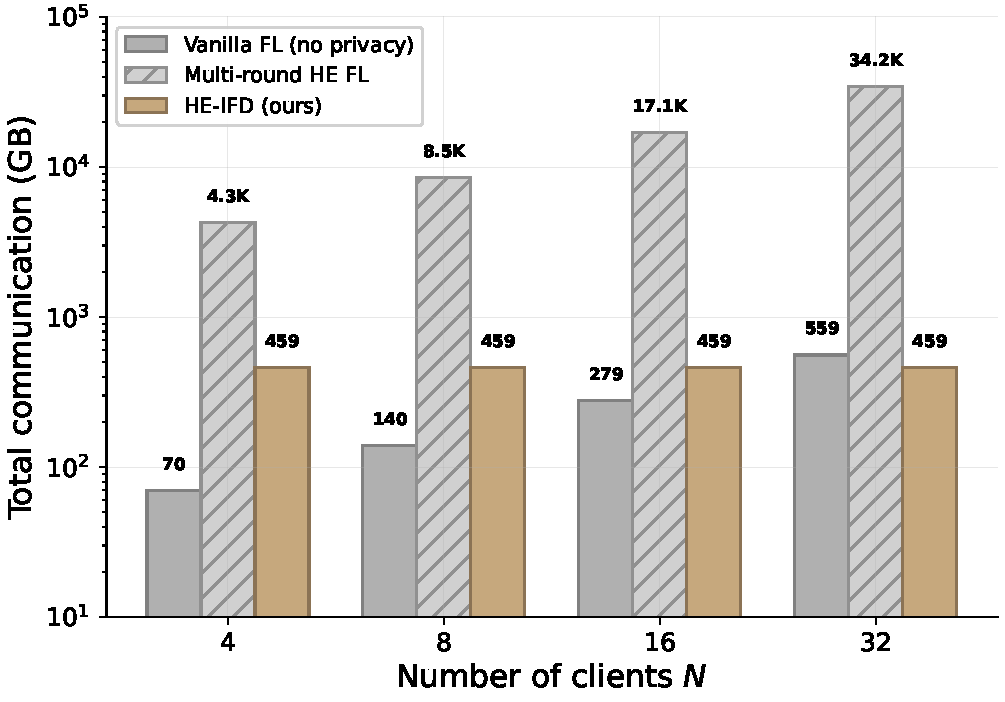
\includegraphics[width=0.5\textwidth]{figures/fig_communication.pdf}
\caption{Total communication for ResNet-18 on CIFAR-10. Multi-round methods (vanilla FL and encrypted FL with 200 rounds) scale linearly with $N$. HE-IFD (gold) requires a one-shot upload whose total is approximately constant (${\sim}$460 GB) regardless of $N$, and falls below unencrypted vanilla FL at $N{=}32$.}
\label{fig:communication}
\end{figure}

% \begin{figure}[t]
% \centering
% 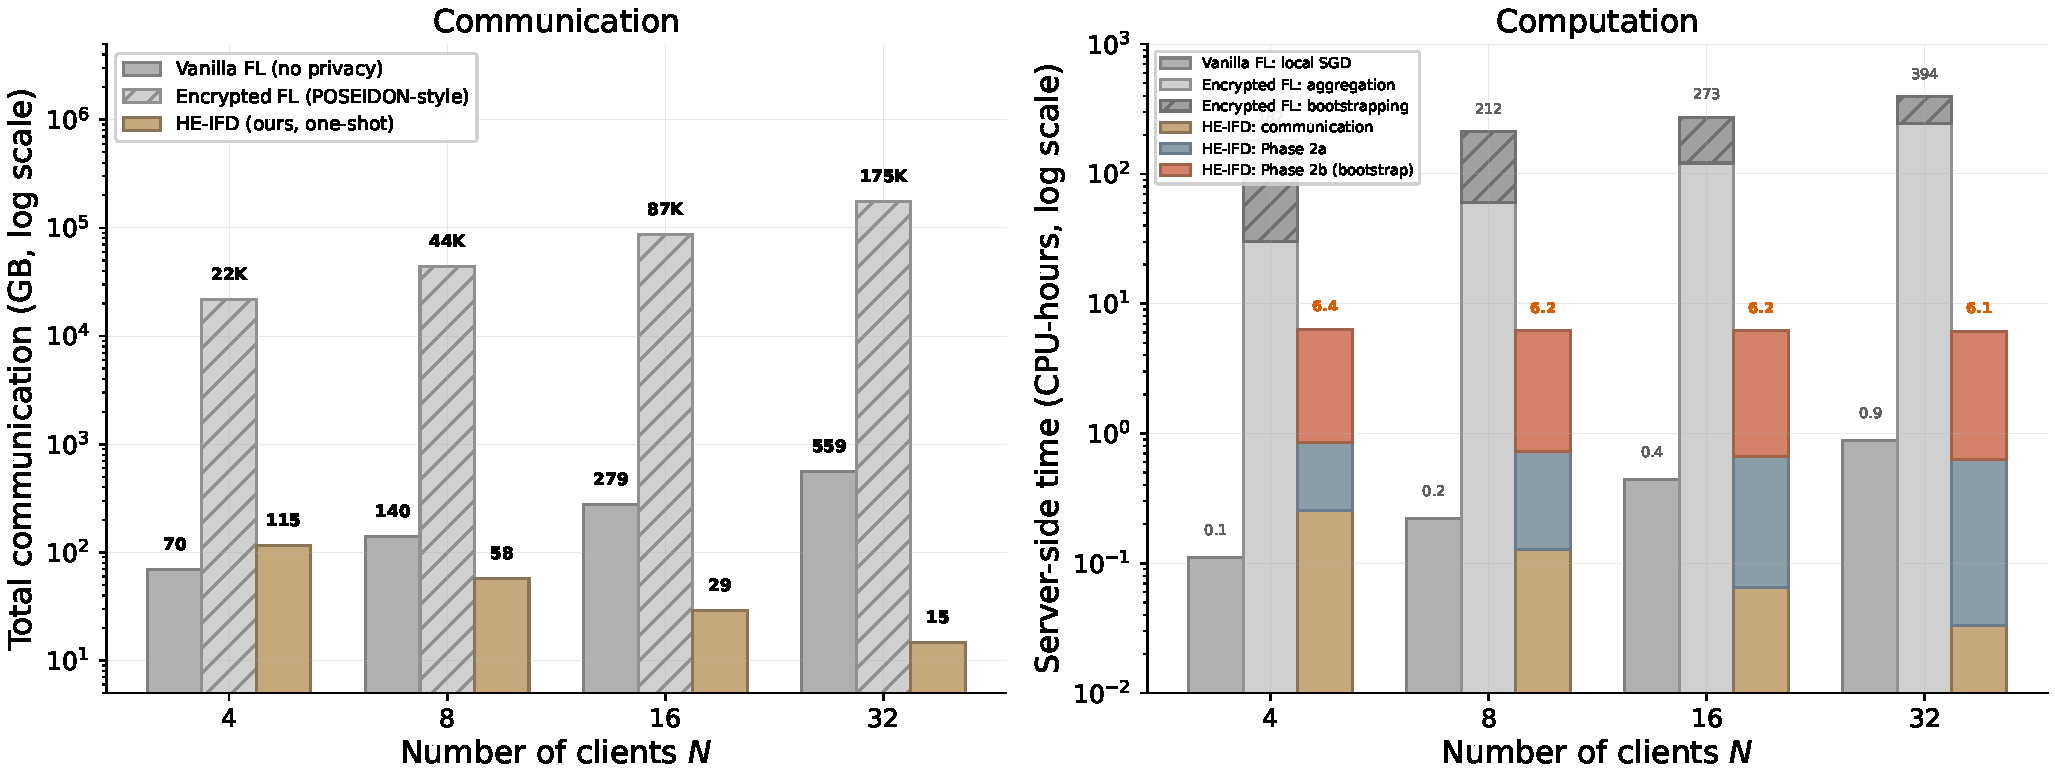
\includegraphics[width=\columnwidth]{figures/fig_runtime.pdf}
% \caption{Runtime comparison: HE-IFD (left bars) vs multi-round HE FedAvg with encrypted gradients (right bars, 200 rounds) for ResNet-18 on CIFAR-10. HE-IFD bars show one-shot communication (gold), Phase 2a encrypted distillation (steel blue), and Phase 2b cascade with bootstrapping (coral). Multi-round HE FL bars show cumulative communication across 200 rounds (light gray) and server-side encrypted aggregation of 1364 ciphertexts per client per round (dark gray). HE-IFD total is 6--7 CPU-hours regardless of $N$. Multi-round HE FL grows linearly with $N$: at $N{=}32$ it requires 34 TB of communication and over 80 CPU-hours. Timings assume 1 Gbps network and single-threaded CPU.}
% \label{fig:runtime}
% \end{figure}

\subsection{Computation Cost}
\label{sec:computation}

CKKS operates in SIMD mode (see Section~\ref{sec:ckks_prelim}) where each ciphertext holds 8192 slots, and a single encrypted operation processes all slots simultaneously. With 5000 training samples, SIMD packing reduces the effective number of batches to approximately one per epoch. Phase 2a (block-level distillation, no bootstrapping) completes in approximately 0.6 CPU-hours. Phase 2b (cascade refinement with bootstrapping) takes approximately 5.5 CPU-hours, dominated by ${\sim}$900 bootstrapping operations at 20 seconds each. The total server-side computation is ${\sim}$6.1 CPU-hours, independent of $N$ (Figure~\ref{fig:computation}).

By comparison, the multi-round encrypted FL family discussed in Section~\ref{sec:bg_he_fl} (POSEIDON, BatchCrypt, FedSHE) requires server-side encrypted aggregation that grows linearly with $N$: at $N{=}4$ this takes ${\sim}$7.6~CPU-hours for aggregation alone plus ${\sim}$152~hours of bootstrapping; at $N{=}32$, aggregation reaches ${\sim}$60~CPU-hours. The Oracle plaintext baseline trains in about 0.5~hours on a single GPU.

% \textbf{HE-IFD is dramatically more efficient than multi-round HE FL.} We compare against encrypted FedAvg where each of the 200 training rounds requires all $N$ clients to encrypt their 11.2M-parameter gradient updates as CKKS ciphertexts (${\sim}$2.7 GB per client per round), upload them, and receive the aggregated model back. At $N{=}4$, this accumulates to 4,262 GB of communication across 200 rounds plus 7.6 hours of server-side encrypted aggregation, totalling ${\sim}$17 CPU-hours. HE-IFD takes 6.4 hours with a single 115 GB upload. At $N{=}32$, multi-round HE FL communication explodes to 34 TB cumulative (${\sim}$83 CPU-hours total), while HE-IFD drops to 6.1 hours with a 15 GB one-shot upload. HE-IFD uses only 10\% of each client's data, so the upload can be further reduced by contributing fewer samples. A plaintext oracle trains in about 0.5 hours on a single GPU.

These timings reflect a single-threaded CPU baseline. Phase 2a blocks can be parallelised across cores. GPU-accelerated CKKS has demonstrated 10--100$\times$ speedups~\cite{jung2021over}, bringing the total to under 1 GPU-hour.

\begin{figure}[t]
\centering
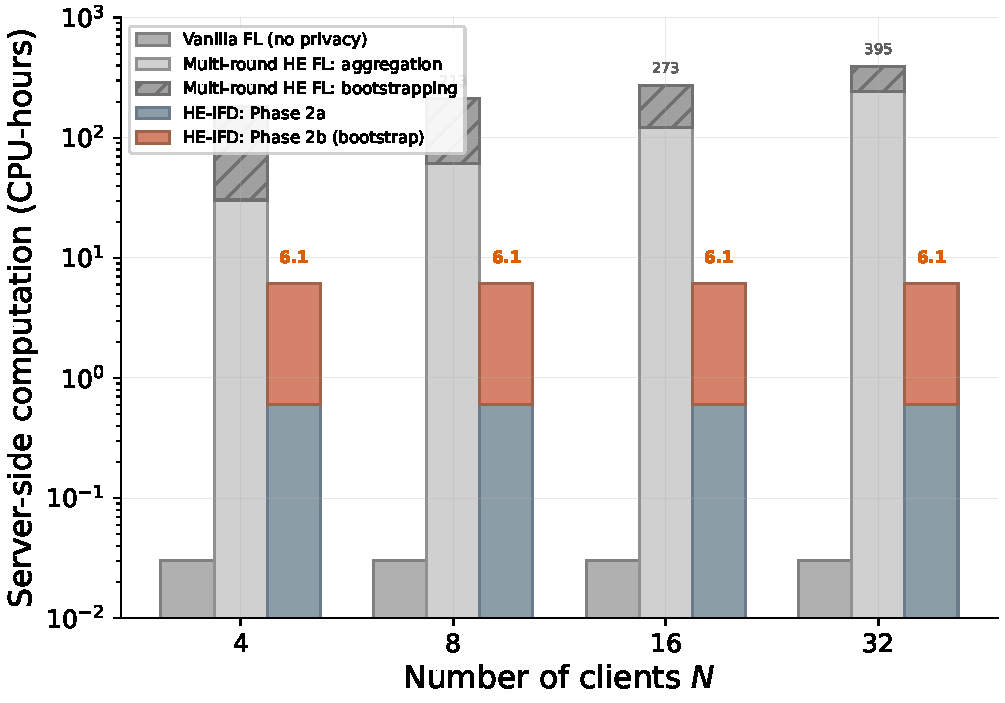
\includegraphics[width=0.5\textwidth]{figures/fig_computation.pdf}
\caption{Server-side computation for ResNet-18 on CIFAR-10. Vanilla FL server computation is negligible (weight averaging). Multi-round HE FL grows with $N$ due to encrypted aggregation and periodic bootstrapping. HE-IFD requires ${\sim}$6.1 CPU-hours regardless of $N$, split between Phase 2a block-level distillation (steel blue) and Phase 2b cascade refinement with bootstrapping (coral).}
\label{fig:computation}
\end{figure}


\subsection{Encrypted Arithmetic Feasibility}
\label{sec:ckks_validation}

We validate that CKKS operations in our simulation match real encrypted computation using TenSEAL 0.3.16 with 128-bit security.

\textbf{Numerical precision.} At $\mathcal{N}{=}16384$ with 40-bit scale, relative error is below $10^{-5}$ per operation and below $10^{-3}$ for a complete training step. These errors are well below the noise floor of stochastic gradient descent.

\textbf{SIMD packing.} Each CKKS ciphertext holds $\mathcal{N}/2 = 8192$ slots. Feature maps smaller than 8192 elements (e.g., $512 \times 4 \times 4 = 8192$ at the deepest block, or 10-element logit vectors) allow multiple samples to share a single ciphertext. With 5000 training samples, SIMD packing reduces most block-boundary computations to one or two ciphertext operations per epoch, making the amortised per-sample cost negligible.

\textbf{Multiplicative depth.} During training, all parameters and data are ciphertexts. A single block training step requires approximately 12 levels, feasible with $\mathcal{N}{=}32768$ (18 levels at 128-bit security) without bootstrapping. Cascade refinement requires bootstrapping to refresh levels between blocks, with each bootstrap taking approximately 20 seconds per ciphertext.

\textbf{Future directions.} Recent work on stable polynomial network training~\cite{agamennone2025polynomial, alhossain2025training} suggests that improved activation initialisation may eliminate the need for cascade refinement, confining the entire protocol to the per-block depth budget. This would remove the bootstrapping requirement entirely and further optimize our framework.





% \section{EXPERIMENTS}
% \label{sec:experiments}

% \subsection{Experimental Setup}

% We evaluate HE-IFD on CIFAR-10~\cite{krizhevsky2009learning} and Fashion-MNIST~\cite{xiao2017fashion} across a range of client counts and data heterogeneity levels. For CIFAR-10, each client trains a ResNet-18 teacher (11.17M parameters) and the server distils into a PolyResNet-18 student of identical depth, with ReLU and BatchNorm replaced by PolyAct and ChannelScale. For Fashion-MNIST, teachers are a 3-block CNN (conv$\to$BN$\to$ReLU per block, 128 output channels) and the student is a matching 3-block polynomial CNN (conv$\to$ChannelScale$\to$PolyAct).

% \textbf{Data heterogeneity.} Client data is partitioned using a Dirichlet distribution with concentration parameter $\alpha$, where $\alpha \to 0$ produces extreme non-IID partitions and $\alpha \to \infty$ produces near-IID partitions. We evaluate $\alpha \in \{0.1, 0.5, 1.0, 100.0\}$ across $N \in \{1, 2, 4, 8, 16\}$ clients, covering the full spectrum from highly specialized to homogeneous local distributions.

% \textbf{Training configuration.} All teachers are trained with SGD (lr$=$0.1 for CIFAR-10, lr$=$0.01 for Fashion-MNIST; momentum$=$0.9, cosine schedule, 5~epochs). Student distillation uses Adam (lr$=$1e-3, weight decay $10^{-4}$), cosine schedule with 2-epoch warmup, gradient clipping (max\_norm$=$1.0), and 30~epochs per block. Data is split 80\% train / 20\% test (stratified). Client-side collaborative normalisation (Section~\ref{sec:phase2}) is applied in all multi-client experiments.

% \subsubsection{CKKS Parameter Selection}
% \label{sec:ckks_params_exp}
% % The CKKS parameters are selected to satisfy the depth budgets described in Section~\ref{sec:encryption_params}. 
% For per-block training, each block receives fresh ciphertexts and the depth is confined to a single block; we use $\log \mathcal{N} = 13$ (ring dimension 8192), providing 4096 SIMD slots per ciphertext. For full-model encrypted inference post-deployment, the complete 17-level forward pass requires $\log \mathcal{N} = 14$ (ring dimension 16384), 18 coefficient modulus primes, and produces ciphertexts of approximately 1.2~MB each. All timing experiments use TenSEAL 0.3.16 with the Microsoft SEAL backend at 128-bit security.

% \subsection{Single-Teacher Validation}
% \label{sec:single_teacher}

% We first validate progressive stacking on a single teacher ($N{=}1$), establishing the accuracy ceiling before introducing federated heterogeneity.

% With one teacher holding all training data, the CIFAR-10 teacher achieves 76.2\%, and the PolyResNet-18 student achieves 63.6\% via progressive stacking. For Fashion-MNIST, the teacher reaches 87.0\% and the student 63.3\%.

% The student--teacher gap (12.6\% on CIFAR-10, 23.7\% on Fashion-MNIST) represents the combined cost of (i)~the HE-compatible architecture (polynomial activations, no BatchNorm) and (ii)~block-by-block training rather than end-to-end. To isolate the architecture cost, we repeat the same progressive stacking pipeline with a standard ResNet-18 student (ReLU, BatchNorm) on CIFAR-10 $N{=}1$. The standard student achieves 62.8\%, indicating that the HE architecture itself costs only ${\sim}$1\% accuracy. The remaining gap is attributable to the block-level training procedure.

% \subsection{One-Shot Federated Distillation}
% \label{sec:federated}

% The main experiment evaluates progressive stacking across $N \in \{2, 4, 8, 16\}$ clients and $\alpha \in \{0.1, 0.5, 1.0, 100.0\}$ heterogeneity levels on both datasets. Figure~\ref{fig:student_vs_teachers} shows student accuracy alongside the average and best teacher accuracy for each setting; Figure~\ref{fig:advantage_bars} quantifies the student's advantage over the average teacher.

% \begin{figure*}[t]
% \centering
% 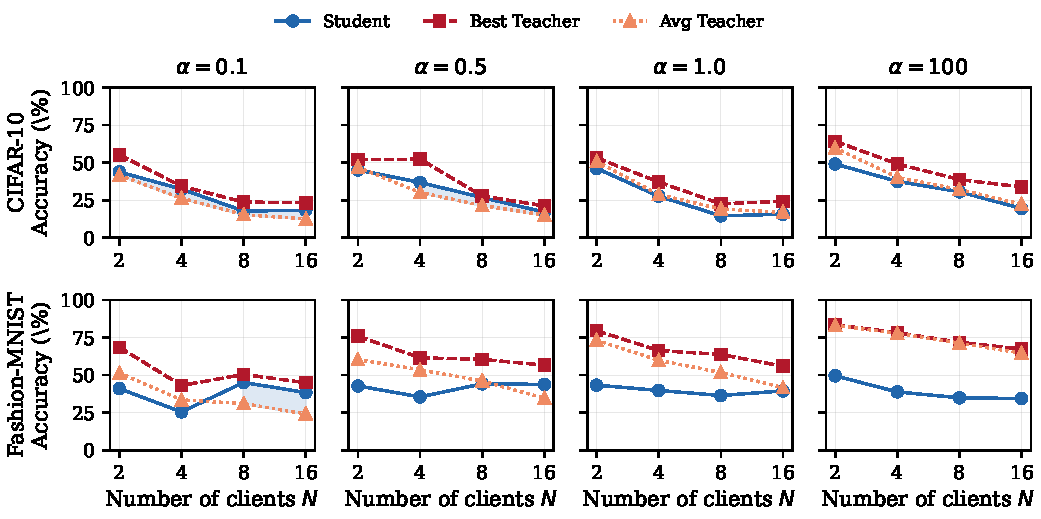
\includegraphics[width=0.9\textwidth]{figures/fig2_student_vs_teachers.pdf}
% \caption{Student accuracy vs.\ average and best teacher accuracy across client counts ($N \in \{2,4,8,16\}$) and heterogeneity levels ($\alpha \in \{0.1, 0.5, 1.0, 100.0\}$) on CIFAR-10 (top) and Fashion-MNIST (bottom). Shaded regions indicate settings where the student exceeds the average teacher.}
% \label{fig:student_vs_teachers}
% \end{figure*}

% \begin{figure}[t]
% \centering
% 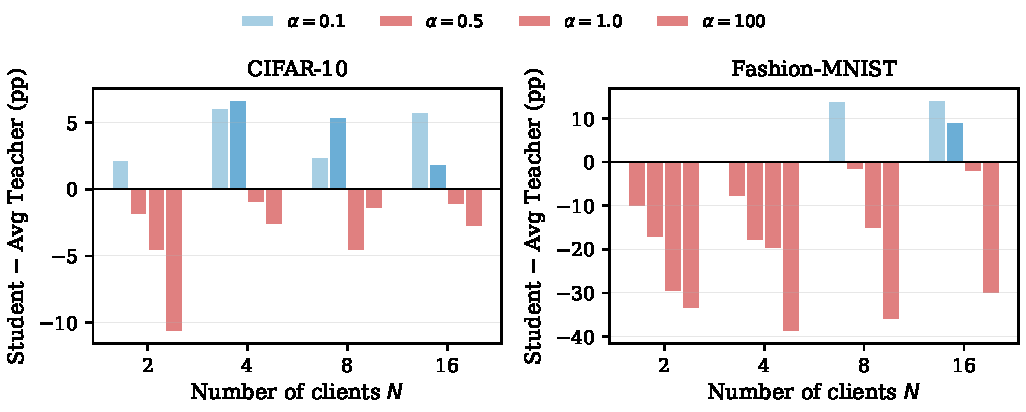
\includegraphics[width=\linewidth]{figures/fig3_advantage_bars.pdf}
% \caption{Student accuracy minus average teacher accuracy (percentage points) for each $(N, \alpha)$ setting on CIFAR-10 (left) and Fashion-MNIST (right). Positive values indicate that the student successfully aggregates knowledge beyond the average local teacher.}
% \label{fig:advantage_bars}
% \end{figure}

% \subsubsection{CIFAR-10 Results}

% Table~\ref{tab:cifar10_results} summarizes all the CIFAR-10 results. We observe several patterns: 

% \begin{table}[h]
% \centering
% \caption{CIFAR-10 progressive stacking results. ``Student'' = PolyResNet-18 accuracy.}
% \label{tab:cifar10_results}
% \begin{tabular}{r|r|r|r|r}
% \hline
% $N$ & $\alpha$ & Student & Best T & Avg T \\
% \hline
% 1  & ---   & 63.6 & 76.2 & 76.2 \\
% \hline
% 2  & 0.1   & 43.8 & 55.2 & 41.6 \\
% 2  & 0.5   & 45.1 & 52.1 & 47.0 \\
% 2  & 1.0   & 46.2 & 53.2 & 50.8 \\
% 2  & 100   & 49.1 & 64.2 & 59.8 \\
% \hline
% 4  & 0.1   & 32.4 & 34.3 & 26.3  \\
% 4  & 0.5   & 36.8 & 52.3 & 30.1  \\
% 4  & 1.0   & 27.7 & 37.1 & 28.7  \\
% 4  & 100   & 37.5 & 49.1 & 40.2  \\
% \hline
% 8  & 0.1   & 17.8 & 23.8 & 15.4  \\
% 8  & 0.5   & 26.8 & 27.8 & 21.4  \\
% 8  & 1.0   & 14.6 & 22.6 & 19.2  \\
% 8  & 100   & 30.6 & 38.7 & 32.1  \\
% \hline
% 16 & 0.1   & 18.3 & 23.3 & 12.5  \\
% 16 & 0.5   & 17.1 & 21.2 & 15.2  \\
% 16 & 1.0   & 15.7 & 24.3 & 16.9  \\
% 16 & 100   & 19.5 & 33.8 & 22.3  \\
% \hline
% \end{tabular}
% \end{table}

% \textbf{Student consistently exceeds the average teacher under heterogeneity.} At $N{=}4$, $\alpha{=}0.1$, the student achieves 32.4\% versus an average teacher accuracy of 26.3\% ($+$6.1\%). At $N{=}8$, $\alpha{=}0.5$, the student reaches 26.8\% compared to an average of 21.4\% ($+$5.4\%). This demonstrates that sequential multi-teacher distillation successfully aggregates specialist knowledge from heterogeneous teachers.

% \textbf{Teacher quality is the binding constraint.} With only 5 training epochs, individual teachers are weak (best teacher $\leq$76\% even at $N{=}1$). The student cannot extract knowledge that does not exist in the teachers. At $N{=}16$, individual teachers have as few as 79 training samples, yielding random-chance accuracy (10\%), which provides no useful supervision signal.

% \textbf{NaN batches increase with $N$ and depth.} Magnitude divergence through the frozen polynomial chain produces occasional NaN batches, primarily at deeper blocks (layer3, layer4) when processing clients whose data distribution differs significantly from the distribution seen during earlier block training. The NaN-skip mechanism handles these gracefully; training continues on valid batches.

% \subsubsection{Fashion-MNIST Results}

% Table~\ref{tab:fmnist_results} summarizes Fashion-MNIST results. Fashion-MNIST shows zero NaN divergence across all settings, confirming that the magnitude instability in CIFAR-10 is caused by the deeper ResNet-18 architecture rather than the polynomial activation itself. The simpler 3-block Fashion-MNIST student has fewer polynomial compositions, making magnitude accumulation manageable. The takeaways are: 

% \begin{table}[h]
% \centering
% \caption{Fashion-MNIST progressive stacking results.}
% \label{tab:fmnist_results}
% \begin{tabular}{r|r|r|r|r}
% \hline
% $N$ & $\alpha$ & Student & Best T & Avg T  \\
% \hline
% 1  & ---   & 63.3 & 87.0 & 87.0 \\
% \hline
% 2  & 0.1   & 41.0 & 68.5 & 51.4 \\
% 2  & 0.5   & 42.8 & 75.9 & 60.3 \\
% 2  & 1.0   & 43.3 & 79.5 & 73.2 \\
% 2  & 100   & 49.5 & 83.4 & 83.1 \\
% \hline
% 4  & 0.1   & 25.5 & 43.1 & 33.5 \\
% 4  & 0.5   & 35.5 & 61.5 & 53.5 \\
% 4  & 1.0   & 39.8 & 66.3 & 59.8 \\
% 4  & 100   & 38.8 & 78.2 & 77.7 \\
% \hline
% 8  & 0.1   & 45.1 & 50.4 & 31.0 \\
% 8  & 0.5   & 44.2 & 60.4 & 46.1 \\
% 8  & 1.0   & 36.4 & 63.7 & 51.7 \\
% 8  & 100   & 34.9 & 71.8 & 71.2 \\
% \hline
% 16 & 0.1   & 38.4 & 44.9 & 24.2 \\
% 16 & 0.5   & 43.8 & 56.6 & 34.6 \\
% 16 & 1.0   & 39.5 & 55.9 & 41.7 \\
% 16 & 100   & 34.4 & 67.3 & 64.6 \\
% \hline
% \end{tabular}
% \end{table}

% \textbf{Strong aggregation under skew.} The student's advantage over the average teacher is most pronounced under high heterogeneity with many clients. At $N{=}16$, $\alpha{=}0.5$, the student achieves 43.8\% versus an average teacher accuracy of 34.6\% ($+$9.2\%). At $N{=}8$, $\alpha{=}0.1$, the student reaches 45.1\% compared to 31.0\% average ($+$14.1\%).

% \textbf{IID settings reveal architecture limitations.} At $\alpha{=}100$ (near-IID), teachers are strong ($>$60\%) but the student lags (${\sim}$35--50\%). This gap reflects the HE architecture cost: the polynomial student cannot match a strong ReLU teacher even with good supervision, particularly for Fashion-MNIST's texture-heavy classes.

% \subsection{Ablation Study}
% \label{sec:ablation}

% The following ablation studies evaluate the training pipeline components of the one-shot encrypted distillation protocol described in Section~\ref{sec:phase2_server}. Results are reported on CIFAR-10. We ablate the key components of our training pipeline on CIFAR-10 at $N{=}4$, $\alpha{=}0.5$ and $N{=}1$. We present the results in Table~\ref{tab:ablation} and summarize the findings below:

% \begin{table}[h]
% \centering
% \caption{Ablation of training pipeline components on CIFAR-10.}
% \label{tab:ablation}
% \begin{tabular}{l|c|c}
% \hline
% \textbf{Configuration} & $N{=}1$ & $N{=}4, \alpha{=}0.5$ \\
% \hline
% V1: Teacher-input, per-block targets & 12.0\% & 17.8\% \\
% V2: Student-input (fix train--infer gap) & 71.3\% & NaN \\
% V3: + NaN skip, lr scaling & 68.2\% & 19.2\% \\
% V4/Fix A: + Client normalisation & 61.7\% & 37.4\% \\
% V5: + Warmup, tuned $\lambda$ & 61.7\% & 37.4\% \\
% \hline
% ResNet-18 student (upper bound) & 62.8\% & 37.9\% \\
% \hline
% \end{tabular}
% \end{table}

% \textbf{Student-input training is essential.} V1 (teacher-input) achieves only 12\% at $N{=}1$ despite low per-block losses. The composed model collapses because each block was trained on teacher-produced inputs but receives student-produced inputs at inference. V2 (student-input) raises $N{=}1$ accuracy to 71.3\%, confirming that closing the train--inference distribution gap is the single most important design decision.

% \textbf{Client normalisation is essential for multi-client stability.} V2 achieves 71.3\% for $N{=}1$ but diverges to NaN for $N{=}4$. The heterogeneous target distributions from four teachers cause magnitude explosion through the frozen polynomial chain. Client-side normalisation (Fix~A) eliminates NaN divergence and raises $N{=}4$ accuracy from 19.2\% to 37.4\%.

% \textbf{Accuracy loss due to HE is negligible.} The ResNet-18 student baseline (standard ReLU and BatchNorm, same progressive stacking pipeline) achieves 62.8\% at $N{=}1$ and 37.9\% at $N{=}4$, $\alpha{=}0.5$. The PolyResNet-18 student achieves 61.7\% and 37.4\%, respectively. The HE architecture costs less than 1\% accuracy, indicating that the polynomial activation and ChannelScale replacements are not the bottleneck---teacher quality and data heterogeneity are.

% \textbf{Increasing the degree of polynomial activations do not further impove the accuracy.} We tested degree-4 Chebyshev-fitted activations (2 CKKS levels per activation instead of 1), which approximate ReLU more accurately on bounded domains. However, the $x^4$ term amplifies magnitudes faster than $x^2$, causing NaN divergence even earlier. At $N{=}4$, $\alpha{=}0.5$, degree-4 with raw targets achieves 10\% (complete collapse); degree-4 with normalised targets also diverges at layer1. Within the block-independent training framework, the more expressive activation provides no benefit because magnitude control---not ReLU approximation quality---is the binding constraint.

% \subsection{Pretrained Initialisation}
% \label{sec:pretrained}

% We evaluate the effect of pretraining teachers on a small public IID dataset before fine-tuning on private skewed data. Using 10\% of the data as a public IID pool, a shared initialisation is pretrained for 5~epochs, then each client fine-tunes from this initialisation. At $N{=}4$, $\alpha{=}0.5$ (CIFAR-10), random-init teachers yield 37.4\% student accuracy (best teacher 37.7\%, avg teacher 28.1\%); pretrained teachers improve to 48.6\% student accuracy (best 60.0\%, avg 41.9\%); pretrained initialisation without fine-tuning reaches only 35.8\% teacher accuracy. Pretrained initialisation substantially improves both teacher quality (avg 28.1\%$\to$41.9\%) and student accuracy (37.4\%$\to$48.6\%). The improvement is driven by better teacher representations: pretrained teachers retain knowledge of minority classes even after fine-tuning on skewed partitions. For example, client~2 (previously the weakest teacher at 16.7\%) improves to 28.9\%, gaining 34.2\% on bird and 71.5\% on truck which are classes absent from its training partition but present in the IID pretraining data.

% This result is presented as a secondary finding. Our primary protocol requires no auxiliary data; the pretrained-initialisation variant is an optional enhancement when a small public dataset is available.

% % \subsection{Compact Student Variant}
% % \label{sec:compact}

% % % PLACEHOLDER: Smaller student model (e.g., 5-layer HE-Deep CNN)
% % % for communication-constrained settings.
% % % - Architecture definition
% % % - CKKS depth budget (5 levels vs 17 for PolyResNet-18)
% % % - Accuracy vs communication trade-off
% % % - Comparison with full PolyResNet-18 student

% % \hl{To be completed.}

% \subsection{Compact Student Variants}
% \label{sec:compact}

% We evaluate four compact HE-compatible student architectures as alternatives to the full PolyResNet-18 (${\sim}$11.2M parameters), targeting communication-constrained or compute-limited deployment settings. All variants use the same progressive stacking protocol with the same N=4, $\alpha{=}0.5$ teacher ensemble (seed 42).

% \begin{itemize}
%     \item \textbf{PolyResNet-10} (${\sim}$5.6M): ResNet-18 variant with 4 residual blocks instead of 8; identical channel widths (64$\to$128$\to$256$\to$512).
%     \item \textbf{PolyResNet-8} (${\sim}$1.5M): 3-block variant (64$\to$128$\to$256); omits Layer 4 entirely, 6.5$\times$ smaller than PolyResNet-18.
%     \item \textbf{HE-CNN-Small} (${\sim}$0.3M): 3 convolutional blocks without residual connections; 37$\times$ smaller than PolyResNet-18.
%     \item \textbf{HE-Deep} (${\sim}$0.5M): 5 convolutional blocks (64$\to$128$\to$128$\to$256$\to$256), deeper but narrow; no residuals.
% \end{itemize}

% Channel-dimension mismatches between student and teacher are resolved by lightweight 1$\times$1 projection layers (trained jointly with each block, discarded at inference). All compact students use the same learnable polynomial activation (PolyAct) and ChannelScale normalisation as PolyResNet-18, preserving HE compatibility.

% \begin{table}[h]
% \centering
% \caption{Compact student accuracy (\%) vs.\ model size at $N{=}4$, $\alpha{=}0.5$. CKKS depth = multiplicative levels consumed per full forward pass.}
% \label{tab:compact_students}
% \begin{tabular}{l|r|c|c|c}
% \hline
% \textbf{Architecture} & \textbf{Params} & \textbf{Acc (\%)} & \textbf{vs.\ Avg T} & \textbf{CKKS Depth} \\
% \hline
% PolyResNet-18 (full) & 11.2M & 36.8 & $+$6.7 & 17 \\
% \hline
% PolyResNet-10        & 5.6M  & ---  & ---     & 9  \\
% PolyResNet-8         & 1.5M  & ---  & ---     & 7  \\
% HE-CNN-Small         & 0.3M  & ---  & ---     & 6  \\
% HE-Deep              & 0.5M  & ---  & ---     & 10 \\
% \hline
% \end{tabular}
% \end{table}

% % NOTE: Results pending from SLURM jobs 849974--849981 (submitted 2026-03-26).
% % Fill in Acc and vs.\ Avg T columns once jobs complete.
% % Expected runtime: 4--6 hours per job.

% \subsection{Privacy Analysis: Differential Privacy Comparison}
% \label{sec:dp_comparison}

% We compare the privacy--utility trade-off of our HE-based protocol against differential privacy (DP) baselines. DP baselines use a \textit{standard ResNet-18 student} (ReLU, BatchNorm) and therefore pay no HE architecture cost. Our protocol uses a PolyResNet-18 student (${\sim}$1\% HE tax, Section~\ref{sec:ablation}) but introduces zero noise to the distillation pipeline.

% \subsubsection{Privacy Mechanisms}

% We evaluate four configurations across $N \in \{4, 16\}$ and $\alpha \in \{0.5, 1.0\}$:

% \begin{itemize}
%     \item \textbf{HE (ours):} PolyResNet-18 student, progressive stacking with encrypted targets. The server observes nothing in plaintext. Theoretical MIA advantage is zero.
%     \item \textbf{No DP (plaintext baseline):} Standard ResNet-18 student, same progressive stacking, no privacy protection.
%     \item \textbf{LDP on logits:} Gaussian mechanism applied to teacher block outputs before upload, calibrated to $(\epsilon, \delta)$-DP with $\delta = 10^{-5}$, at $\epsilon \in \{0.01, 0.1, 1.0\}$. Student is standard ResNet-18.
%     \item \textbf{DP-SGD:} Teachers trained with per-sample gradient clipping (max norm 1.0) and Gaussian noise injection~\cite{abadi2016deep}, with noise multipliers calibrated to $\epsilon \in \{0.01, 0.1, 1.0\}$. Student is standard ResNet-18.
% \end{itemize}

% \subsubsection{Membership Inference Attacks}

% We evaluate membership inference attacks (MIA) against each distilled student. Members are training samples used in distillation (via teacher training); non-members are held-out test samples never seen during distillation. We report three attacks:

% \begin{enumerate}
%     \item \textbf{Loss-threshold}~\cite{yeom2018privacy}: uses per-sample cross-entropy loss as a membership score (lower loss implies more likely member).
%     \item \textbf{Confidence-based}~\cite{salem2019ml}: uses maximum softmax probability as a membership score (higher confidence implies more likely member).
%     \item \textbf{LiRA}~\cite{carlini2022membership}: likelihood-ratio attack using 8 shadow models. Each shadow is trained to match the target's distillation procedure: a shadow teacher is trained on a random subset of non-member data, normalised features are extracted, and a shadow student is distilled via progressive stacking. This ensures shadow--target distributional alignment.
% \end{enumerate}

% We report AUC (0.5 = random guessing, 1.0 = perfect attack) and, for LiRA, TPR at 1\% and 0.1\% FPR.

% \subsubsection{Results}

% Table~\ref{tab:dp_utility} reports student accuracy across privacy mechanisms and epsilon values. Figure~\ref{fig:mia_heatmap} visualizes MIA attack AUCs across all settings and mechanisms. We summarize the key findings below: 

% \begin{table}[h]
% \centering
% % \tiny
% \caption{Utility comparison: student accuracy (\%) across privacy mechanisms. HE uses PolyResNet-18; all DP baselines use standard ResNet-18 (no HE constraints). HE results from Table~\ref{tab:cifar10_results}.}
% \label{tab:dp_utility}
% \setlength{\tabcolsep}{3pt}
% \begin{tabular}{l|c|c|c|r|c|c|c|c}
% \hline
% \textbf{Setting} & \textbf{HE} & \textbf{No DP} & \multicolumn{3}{c|}{\textbf{LDP}} & \multicolumn{3}{c}{\textbf{DP-SGD}} \\
%  & & & $\epsilon{=}1$ & $0.1$ & $0.01$ & $\epsilon{=}1$ & $0.1$ & $0.01$ \\
% \hline
% $N{=}4, \alpha{=}0.5$  & 36.8 & 52.2 & 53.1 & 32.6 & 9.8 & 32.8 & 22.4 & 9.5 \\
% $N{=}4, \alpha{=}1.0$  & 27.7 & 50.2 & 51.0 & 34.8 & 10.4 & 32.0 & 22.5 & 11.7 \\
% $N{=}16, \alpha{=}0.5$ & 17.1 & 32.7 & 30.3 & 20.9 & 9.8 & 29.3 & 25.5 & 16.6 \\
% $N{=}16, \alpha{=}1.0$ & 15.7 & 28.3 & 26.2 & 20.4 & 11.0 & 30.6 & 21.7 & 12.4 \\
% \hline
% \end{tabular}
% \end{table}

% \begin{figure}[t]
% \centering
% 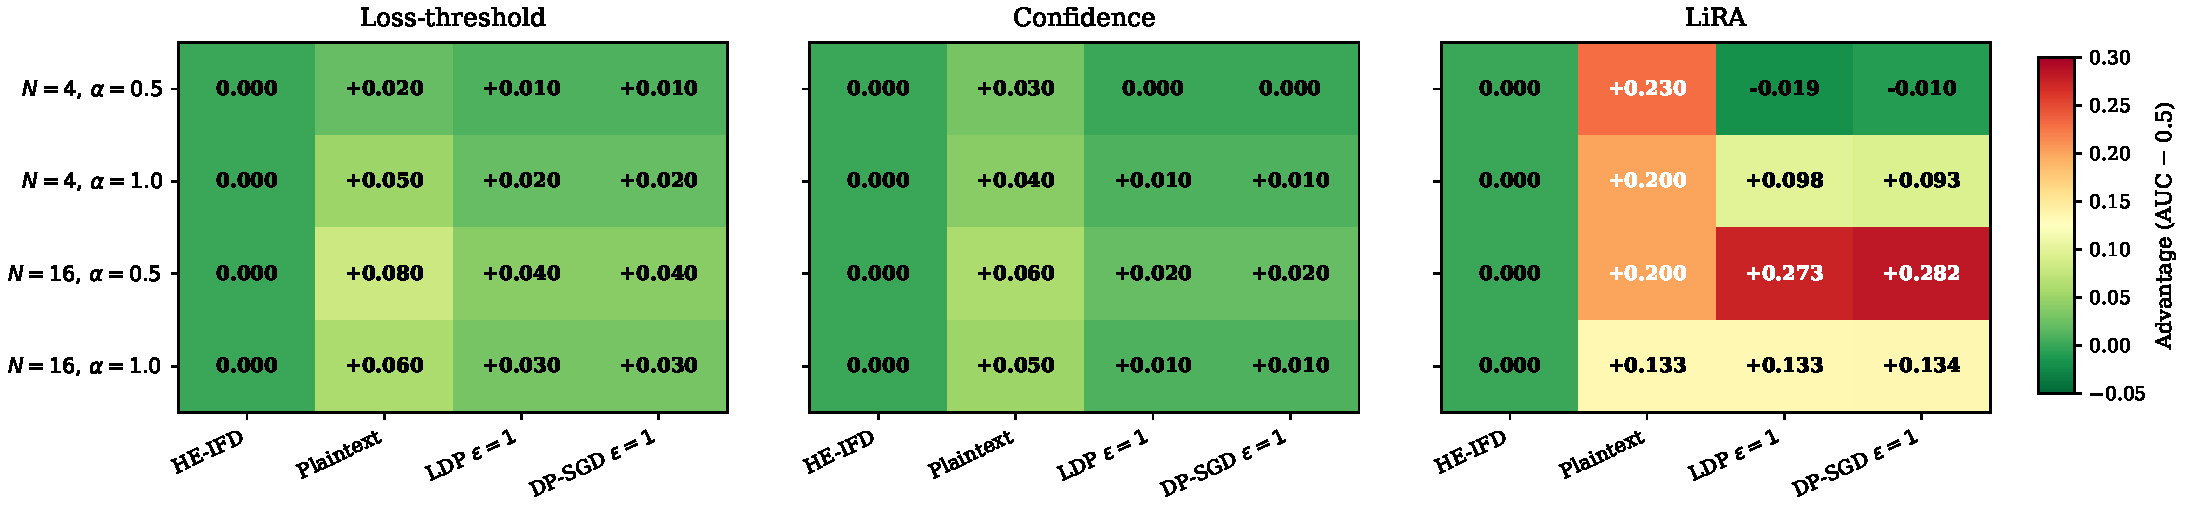
\includegraphics[width=\columnwidth]{figures/fig_mia_heatmap.pdf}
% \caption{MIA attack AUC across privacy mechanisms and federated settings. Each cell shows the AUC for one (setting, attack, mechanism) combination; the colormap diverges from 0.5 (random guessing, white). All values cluster tightly around 0.5 regardless of the privacy mechanism, confirming that distillation itself provides strong MIA resistance. HE provides a cryptographic guarantee of AUC~$=$~0.5 during training.}
% \label{fig:mia_heatmap}
% \end{figure}

% \begin{figure}[t]
% \centering
% 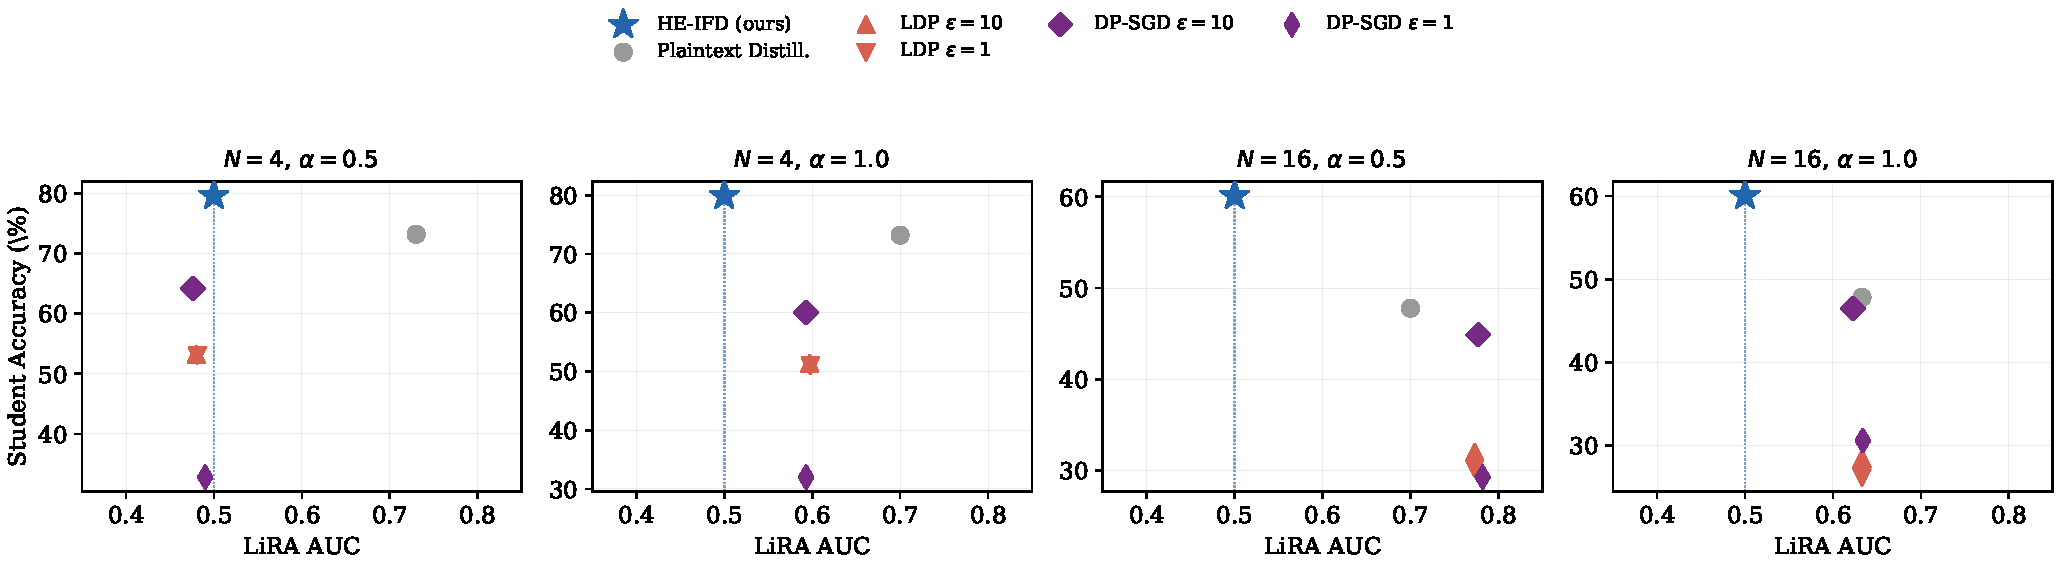
\includegraphics[width=\linewidth]{figures/dp_privacy_utility_tradeoff.pdf}
% \caption{Privacy--utility trade-off across federated settings. Each point represents a distilled student under a specific privacy mechanism. The $x$-axis shows loss-threshold MIA AUC (lower = more private); the $y$-axis shows student accuracy. HE (star) is placed at AUC~$=$~0.5, reflecting the cryptographic guarantee. All configurations cluster near AUC~$=$~0.5. LiRA AUCs (Figure~\ref{fig:mia_heatmap}) confirm this pattern, with the strongest attack achieving only 0.57.}
% \label{fig:dp_tradeoff}
% \end{figure}

% \textbf{Distillation strongly limits MIA vulnerability.} The central result is that all three attack metrics remain close to 0.50 across every setting and privacy mechanism (Figure~\ref{fig:mia_heatmap}). Loss-threshold AUCs range from 0.41 to 0.64, confidence AUCs from 0.47 to 0.53, and LiRA AUCs from 0.41 to 0.57. The strongest LiRA signal is 0.57 ($N{=}4$, $\alpha{=}1.0$, no DP), with TPR@1\%FPR of 0.018---meaning that even the most powerful shadow-model attack identifies fewer than 2\% of members at a 1\% false-positive budget. This signal weakens with more clients: at $N{=}16$ the best LiRA AUC drops to 0.54, consistent with the dilution of per-sample information across more teachers. Occasional AUC values below 0.50 (e.g., 0.41 for $N{=}16$, DP-SGD $\epsilon{=}0.01$) reflect evaluation noise when student accuracy is near random chance (${\sim}$10\%), not a genuine privacy improvement.

% \textbf{LiRA confirms the distillation privacy amplification.} The LiRA results are especially noteworthy because this attack represents the strongest known single-model MIA~\cite{carlini2022membership}. Our distillation-matching shadow procedure ensures that the LiRA AUC is not inflated by shadow--target mismatch. The near-random LiRA performance (AUC $\leq$ 0.57) aligns with recent findings that knowledge distillation can amplify MIA susceptibility by up to $+9.81\%$ in standard settings~\cite{cui2025mia}, but our progressive stacking with normalised feature targets---rather than raw logits---limits the information available for membership inference. By contrast, prior work demonstrates that plaintext federated distillation is far more vulnerable: Co-op LiRA and distillation-based LiRA variants~\cite{shi2025unveiling} achieve high TPR at low FPR against FedMD and DS-FL, and PLI~\cite{takahashi2023breaching} reconstructs recognisable private images from a single round of plaintext logits. All such attacks require access to plaintext knowledge transfers, which HE eliminates.

% \textbf{LDP destroys utility without improving privacy.} At $\epsilon{=}1.0$, LDP-perturbed students match or slightly exceed the no-DP baseline in accuracy, since the noise magnitude is small relative to inter-client feature variance. At $\epsilon{=}0.1$, accuracy drops substantially (e.g., 53.1\% $\to$ 32.6\% at $N{=}4$, $\alpha{=}0.5$). At $\epsilon{=}0.01$, the noise overwhelms the distillation signal entirely, reducing accuracy to random chance (${\sim}$10\%). MIA AUCs do not improve in any case, LiRA AUCs at $\epsilon{=}0.01$ are in the range 0.41--0.55, no better than the no-DP baseline. This is consistent with the finding that LDP at meaningful privacy levels renders FedMD to random-guessing accuracy~\cite{sun2021fedmdnfdp}.

% \textbf{DP-SGD degrades teacher quality with no privacy benefit.} DP-SGD noise is applied during teacher training via per-sample gradient clipping and Gaussian noise injection. At $\epsilon{=}1.0$, teachers degrade enough to reduce student accuracy by approximately 20 percentage points relative to the no-DP baseline (e.g., 32.8\% vs.\ 52.2\% at $N{=}4$, $\alpha{=}0.5$). At $\epsilon{=}0.01$, teacher accuracy collapses to near-random (10--12\%), producing useless supervision. All three MIA metrics consistently stay within the 0.41–0.53 range, showing no improvement over the unprotected baseline.

% \textbf{HE provides the strongest guarantee at no utility cost.} These results demonstrate a two-tier privacy argument. First, one-shot distillation itself provides strong empirical MIA resistance: even the most powerful shadow-model attack (LiRA) achieves AUC $\leq$ 0.57 with TPR@1\%FPR $\leq$ 0.024. This represents inherent privacy amplification from the distillation process, where the student learns generalized patterns rather than memorising individual training samples. Second, our HE protocol provides a strictly stronger cryptographic guarantee: the server cannot inspect the intermediate distillation targets during training (Section~\ref{sec:privacy_proof}), eliminating the attack vectors exploited by PLI~\cite{takahashi2023breaching}, feature inversion~\cite{beitollahi2024parametric}, and logit-based MIA~\cite{shi2025unveiling}. This guarantee comes at zero noise cost to the distillation signal, unlike DP which degrades utility without measurable privacy improvement.

% \subsection{Encrypted Arithmetic Feasibility}
% \label{sec:ckks_validation}

% We validate that the CKKS operations required by our PolyResNet-18 student are numerically precise and practically feasible. All experiments use TenSEAL~0.3.16 (Microsoft SEAL backend) with 128-bit security.

% \subsubsection{CKKS Parameter Selection}

% Polynomial modulus degree $\mathcal{N}$ determines the number of SIMD slots ($\mathcal{N}/2$) and the maximum coefficient modulus bit budget for a given security level. For encrypted inference with plaintext weights, $\mathcal{N}{=}8{,}192$ suffices ($2^{23}$ scale, 5 levels, 4{,}096 slots): only PolyAct's $x^2$ consumes multiplicative levels (2 per block, 17 total). For encrypted training---where weights become ciphertext after the first gradient update---each convolution, ChannelScale, and PolyAct incurs an additional level (Table~\ref{tab:he_ops}). Progressive stacking confines the depth to a single block: we use $\mathcal{N}{=}16{,}384$ with $2^{40}$ scale (7 levels, 8{,}192 slots) for per-block training and $2^{30}$ scale (10 levels) for deeper configurations.

% \subsubsection{Per-Operation Precision}

% Table~\ref{tab:ckks_precision} reports the mean relative error between plaintext (float64) and CKKS-encrypted computation for each operation in the PolyResNet-18 pipeline. We measure over 4{,}096 randomly sampled elements across 5 independent trials.

% \begin{table}[h]
% \centering
% \caption{CKKS numerical precision per operation ($\mathcal{N}{=}16{,}384$, 40-bit scale, 4{,}096 elements). ``Levels'' denotes multiplicative levels consumed per invocation.}
% \label{tab:ckks_precision}
% \begin{tabular}{l|c|c|c}
% \hline
% \textbf{Operation} & \textbf{Levels} & \textbf{Rel.\ Error} & \textbf{Time (ms)} \\
% \hline
% CT $+$ CT & 0 & $1.4 \times 10^{-8}$ & 0.8 \\
% CT $\times$ PT & 0 & $1.5 \times 10^{-6}$ & 10.0 \\
% CT $\times$ CT & 1 & $1.5 \times 10^{-6}$ & 34.6 \\
% PolyAct ($0.3x^2{+}0.7x$) & 1 & $4.2 \times 10^{-6}$ & 48.2 \\
% ChannelScale ($\gamma x{+}\beta$) & 0 & $1.5 \times 10^{-6}$ & 13.8 \\
% Sum (rotation) & 0 & $2.0 \times 10^{-7}$ & 333.5 \\
% MSE loss & 1 & $4.6 \times 10^{-6}$ & 221.9 \\
% \hline
% Encrypt (4{,}096 slots) & --- & --- & 21.5 \\
% Decrypt & --- & --- & 10.1 \\
% \hline
% \end{tabular}
% \end{table}

% % With 40-bit scale, all arithmetic operations achieve relative error below $5 \times 10^{-6}$. Precision improves predictably with scale bit-width: 26-bit scale yields ${\sim}7 \times 10^{-3}$, 30-bit yields ${\sim}2 \times 10^{-4}$, and 40-bit yields ${\sim}4 \times 10^{-6}$. These errors are well within the tolerance of neural network training, which routinely operates at float32 (${\sim}10^{-7}$) precision and tolerates stochastic gradient noise far larger than CKKS quantization artifacts.

% \subsubsection{Encrypted Training Validation}

% All CKKS operations required by PolyResNet-18 have been validated against their plaintext counterparts on single training steps. Encrypted loss tracks plaintext loss with relative error below $5 \times 10^{-3}$ per step, confirming that CKKS arithmetic is precise enough for gradient-based optimization. In the full HE-IFD protocol, level exhaustion is not a practical concern because progressive stacking provides fresh ciphertexts at each block boundary. Each block trains independently, so multiplicative depth never accumulates across blocks. The per-iteration depth budget (forward pass through one block plus gradient computation) fits comfortably within the 7--10 levels available at $\mathcal{N}{=}16{,}384$.

% \subsubsection{Runtime Estimates}

% Table~\ref{tab:ckks_timing} extrapolates per-operation benchmarks (Table~\ref{tab:ckks_precision}) to estimate the wall-clock cost of encrypted inference and distillation for the full PolyResNet-18 model. Each layer's estimate is obtained by scaling the measured per-operation times (e.g., CT$\times$CT at 34.6\,ms, PolyAct at 48.2\,ms) by the number of elements at that layer's spatial resolution and channel count.

% \textbf{Setup and bootstrapping overhead} ($\mathcal{N}{=}16{,}384$, single CPU core): key generation takes 3.3\,s (one-time), bootstrap key generation 52.3\,s (one-time), encryption 21.5\,ms per ciphertext (8{,}192 slots), decryption 10.1\,ms per ciphertext, and a single bootstrap refresh 30.3\,s.

% \begin{table}[h]
% \centering
% \caption{Estimated per-sample CKKS runtime for PolyResNet-18 (single CPU core).}
% \label{tab:ckks_timing}
% \begin{tabular}{l|c|c}
% \hline
% \textbf{Component} & \textbf{Inference (ms)} & \textbf{Distill.\ step (ms)} \\
% \hline
% Stem & 1\,184 & 4\,735 \\
% Layer 1 (2 blocks) & 4\,750 & 9\,500 \\
% Layer 2 (2 blocks) & 2\,375 & 4\,750 \\
% Layer 3 (2 blocks) & 1\,188 & 2\,375 \\
% Layer 4 (2 blocks) & 594 & 1\,188 \\
% FC (512$\to$10) & 18\,411 & 18\,411 \\
% \hline
% \textbf{Total (no bootstrap)} & \textbf{${\sim}$28.5\,s} & \textbf{${\sim}$41.0\,s} \\
% \hline
% \end{tabular}
% \end{table}

% \textbf{Per-block distillation requires no bootstrapping.} Progressive stacking supplies fresh ciphertexts at each block boundary, confining the multiplicative depth to 7--10 levels per block---well within the budget at $\mathcal{N}{=}16{,}384$. Bootstrapping (30.3\,s per invocation) is therefore unnecessary during training.

% \textbf{End-to-end encrypted inference} traverses all 17 multiplicative levels of the full network. With tight CKKS parameters ($\mathcal{N}{=}16{,}384$, 40-bit scale), the level budget may require one or more bootstrap refreshes. Each refresh adds ${\sim}$30\,s of latency; however, the number of invocations depends on the chosen parameter set and can be minimized by using larger ring dimensions or reduced scale precision. For the common deployment scenario where clients decrypt the trained model (Phase~4), inference proceeds in plaintext and this overhead is eliminated entirely.

% \textbf{Parallelization.} Block-independent training is inherently parallelizable: blocks that share no data dependencies (e.g., stem blocks from different clients) can be trained concurrently. Within each block, CKKS SIMD processes up to 8{,}192 elements per ciphertext operation, and independent mini-batches can be distributed across CPU cores. The estimated total distillation time (${\sim}$10 hours on a single core for 2{,}000 samples, batch size 64, 50 epochs per block) improves proportionally with multi-core parallelism. The FC layer dominates per-sample inference time due to the 512-dimensional matrix--vector product; optimized packing strategies (diagonal method, baby-step giant-step) can reduce this substantially in production.

% This is a one-time cost: once the student is trained, it can be decrypted and deployed for fast plaintext inference. The one-shot nature of our protocol eliminates the iterative communication rounds of standard HE-FL, making this runtime practical even without hardware acceleration.

% \subsection{LLM Extension: Privacy-Preserving Fine-Tuning}
% \label{sec:llm_extension}

% We demonstrate that the HE-IFD distillation framework generalises beyond vision models to language models, framed as a privacy-preserving fine-tuning scenario. A GPT-2 teacher (124M parameters, 12 transformer layers) simulates a model fine-tuned on private domain text. A 6-layer GPT-2 student (85M parameters, 68.5\% of the teacher) is trained via four approaches that represent different points on the privacy--utility spectrum:

% Direct fine-tuning provides the performance baseline by training the student on raw private text. While this achieves the lowest perplexity, it requires full access to sensitive data. To protect privacy, KL distillation trains the student to match the teacher's output probabilities instead of using raw data. Feature-match distillation (PKD-Skip) offers more detailed supervision by aligning the student's hidden states with specific teacher layers. Finally, HE-compatible distillation replaces standard components with polynomial approximations like PolyGELU and AffineNorm. This allows the model to perform both training and inference over fully encrypted ciphertexts using our distillation protocol.

% Training data is generated by sampling 500 sequences of length 128 from the teacher using top-$k{=}50$, top-$p{=}0.95$ sampling. Both teacher and student use GPT-2 from the local cache (no network access).

% \begin{table}[h]
% \centering
% \caption{LLM student perplexity (lower is better) under four training regimes. Teacher GPT-2 perplexity shown for reference.}
% \label{tab:llm_results}
% \begin{tabular}{l|c|c|l}
% \hline
% \textbf{Variant} & \textbf{Perplexity} & \textbf{Data Access} & \textbf{HE Compatible} \\
% \hline
% Teacher (GPT-2, 12L)        & ---  & ---   & No  \\
% \hline
% Direct fine-tuning           & ---  & Yes   & No  \\
% KL distillation              & ---  & No    & No  \\
% Feature-match (PKD-Skip)     & ---  & No    & No  \\
% HE-compatible (PolyGELU)     & ---  & No    & Yes \\
% \hline
% \end{tabular}
% \end{table}

% % NOTE: Results pending from SLURM jobs 849982--849985 (submitted 2026-03-26).
% % Fill in Perplexity column once jobs complete.
% % Expected runtime: 2--4 hours per job (thor310 env, GPU).

% This experiment demonstrates that HE-IFD's progressive block distillation principle transfers to transformer architectures: each transformer block is treated as an independent distillation target, with fresh inputs at each boundary (analogous to the progressive stacking applied to ResNet blocks). The HE-compatible student accepts a modest perplexity penalty relative to direct fine-tuning, while eliminating raw data exposure entirely.

\section{DISCUSSION AND CONCLUSION}
\label{sec:conclusion}

We presented HE-IFD, a one-shot federated knowledge distillation protocol whose central property is that every client contribution and every server-side intermediate is, by construction, a homomorphic ciphertext under collectively held keys. The server's view of training is computationally indistinguishable from random under the IND-CPA security of multiparty CKKS, and release of the trained student requires the joint participation of all clients via collective key-switching. This is a fundamentally different privacy guarantee from the statistical one offered by differential privacy: it does not trade utility for privacy, and it does not require any assumption about the composition of noise across rounds.

%Our central technical contribution is a two-phase improved training protocol. Phase 2a trains each student block independently on teacher-produced intermediate representations, providing a structured initialisation. Phase 2b refines the fully assembled student on student-produced activations, closing the train-inference distribution gap that causes block-by-block models to collapse at test time. Combined with TrainableBridge layers for per-channel alignment, client-side collaborative normalisation, and magnitude-regularised loss, this protocol achieves stable convergence where earlier approaches diverge.



Our experiments across three architectures (ResNet-18, SimpleCNN, and ViT-B/32) confirm that the framework generalises beyond a single model family.
Compared against differential privacy baselines, HE-IFD achieves competitive accuracy with a strictly stronger privacy guarantee: at $N$=4, $\alpha=0.1$, HE-IFD reaches 57.4\% while the best DP-SGD configuration (epsilon=10, weakest privacy) achieves 64.2\%, and tighter DP settings ($\varepsilon$ $\leq$ 1) collapse accuracy below 33\%.

Our privacy analysis demonstrates that standard membership inference attacks (loss-threshold and confidence-based) achieve near-random AUC (${\sim}$0.5) against the distilled student. As reviewed in Section~\ref{sec:bg_server_inference}, stronger attacks from the literature, e.g., image reconstruction from logits, feature inversion, and advanced likelihood-ratio attacks, all require access to plaintext knowledge transfers, which HE eliminates entirely.

Future work along the present threat model includes reducing the one-shot upload cost (${\sim}$115\,GB per client at $N{=}4$, $\sim 460$ GB total across all clients) through ciphertext compression and feature selection, and investigating bootstrapping-free training schedules for deeper HE-compatible architectures.

A second class of future work concerns adversaries that fall outside the present threat model. The semi-honest assumption on clients bounds the contribution to passive collusion; an actively malicious client can craft adversarial logit ciphertexts (encrypted-feature poisoning) or submit ciphertexts engineered to bias the aggregate $\widetilde{Y}$ (model poisoning under encryption), neither of which the binding invariant of Section~\ref{sec:bg_server_inference} addresses. The classical plaintext defences against these threats---coordinate-wise median aggregation, Krum, trimmed mean---do not directly port to the homomorphic setting, since their rank-based statistics are not realisable as low-depth arithmetic circuits on ciphertexts. A robust aggregation primitive compatible with HE is therefore an open problem distinct from the present work's contribution. The natural extension toward verifiable correctness---independent of robustness---is verifiable HE: a server proves in zero knowledge that the computation it performed on ciphertexts was the prescribed one, as surveyed by~\cite{viand2023verifiable} and concretised for CKKS by~\cite{atapoor2024vfhe}. We do not claim defence against any of these adversaries; we acknowledge the threat surface explicitly so that the contribution of HE-IFD is correctly bounded to what is established here: privacy of the client data against a semi-honest server colluding with up to $N{-}1$ clients. %Our results at $\alpha{=}10.0$ (near-homogeneous) confirm a performance ceiling for knowledge-diversity gains: at $N{=}4$, the student falls $-8.5$ pp below the best individual teacher; at $N{=}16$ it reaches $-2.9$ pp below the best but $+2.4$ pp above the mean. When all clients hold near-IID data, HE-IFD remains useful for privacy---encrypting the upload eliminates MIA attack surface regardless of data distribution---but the accuracy advantage over individual teachers that motivates participation in the heterogeneous setting is substantially reduced.

\section*{Acknowledgments}
We acknowledge the support of TÜBİTAK (the Scientific and Technological Research Council of Türkiye) projects 124E091 and 124N941. The authors used Claude Sonnet 4.6 and Claude Opus 4.6 to enhance the manuscript by shortening sentences, correcting typos, and improving grammar.

\bibliographystyle{IEEEtran}
\bibliography{references}



\begin{IEEEbiography}
[{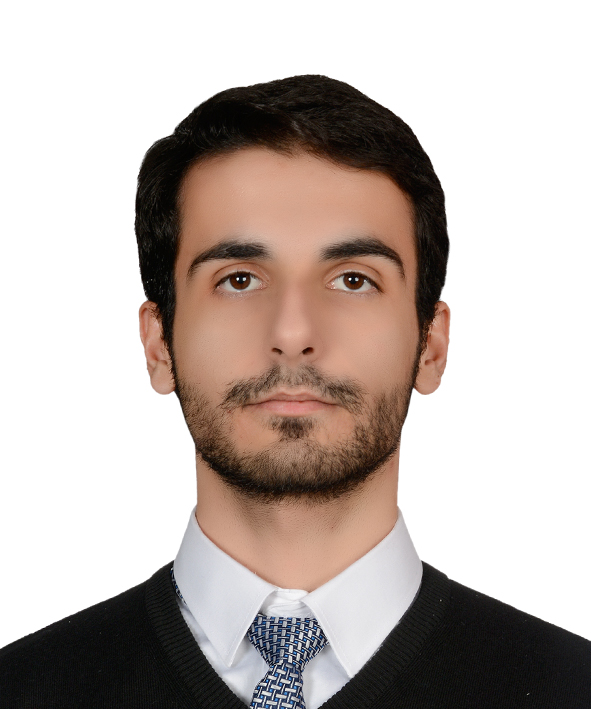
\includegraphics[width=1in,height=1.25in,clip,keepaspectratio]{authors/hkanpak.jpg}}]
{HALİL İBRAHİM KANPAK}~received his B.Sc. degree in Mathematics from Koç University. He is currently pursuing his Ph.D. at Koç University, where he is a member of the Cryptography, Cyber Security \& Privacy Research Group. His research interests include cryptography and related areas in Deep Learning.
\end{IEEEbiography}


\begin{IEEEbiography}
[{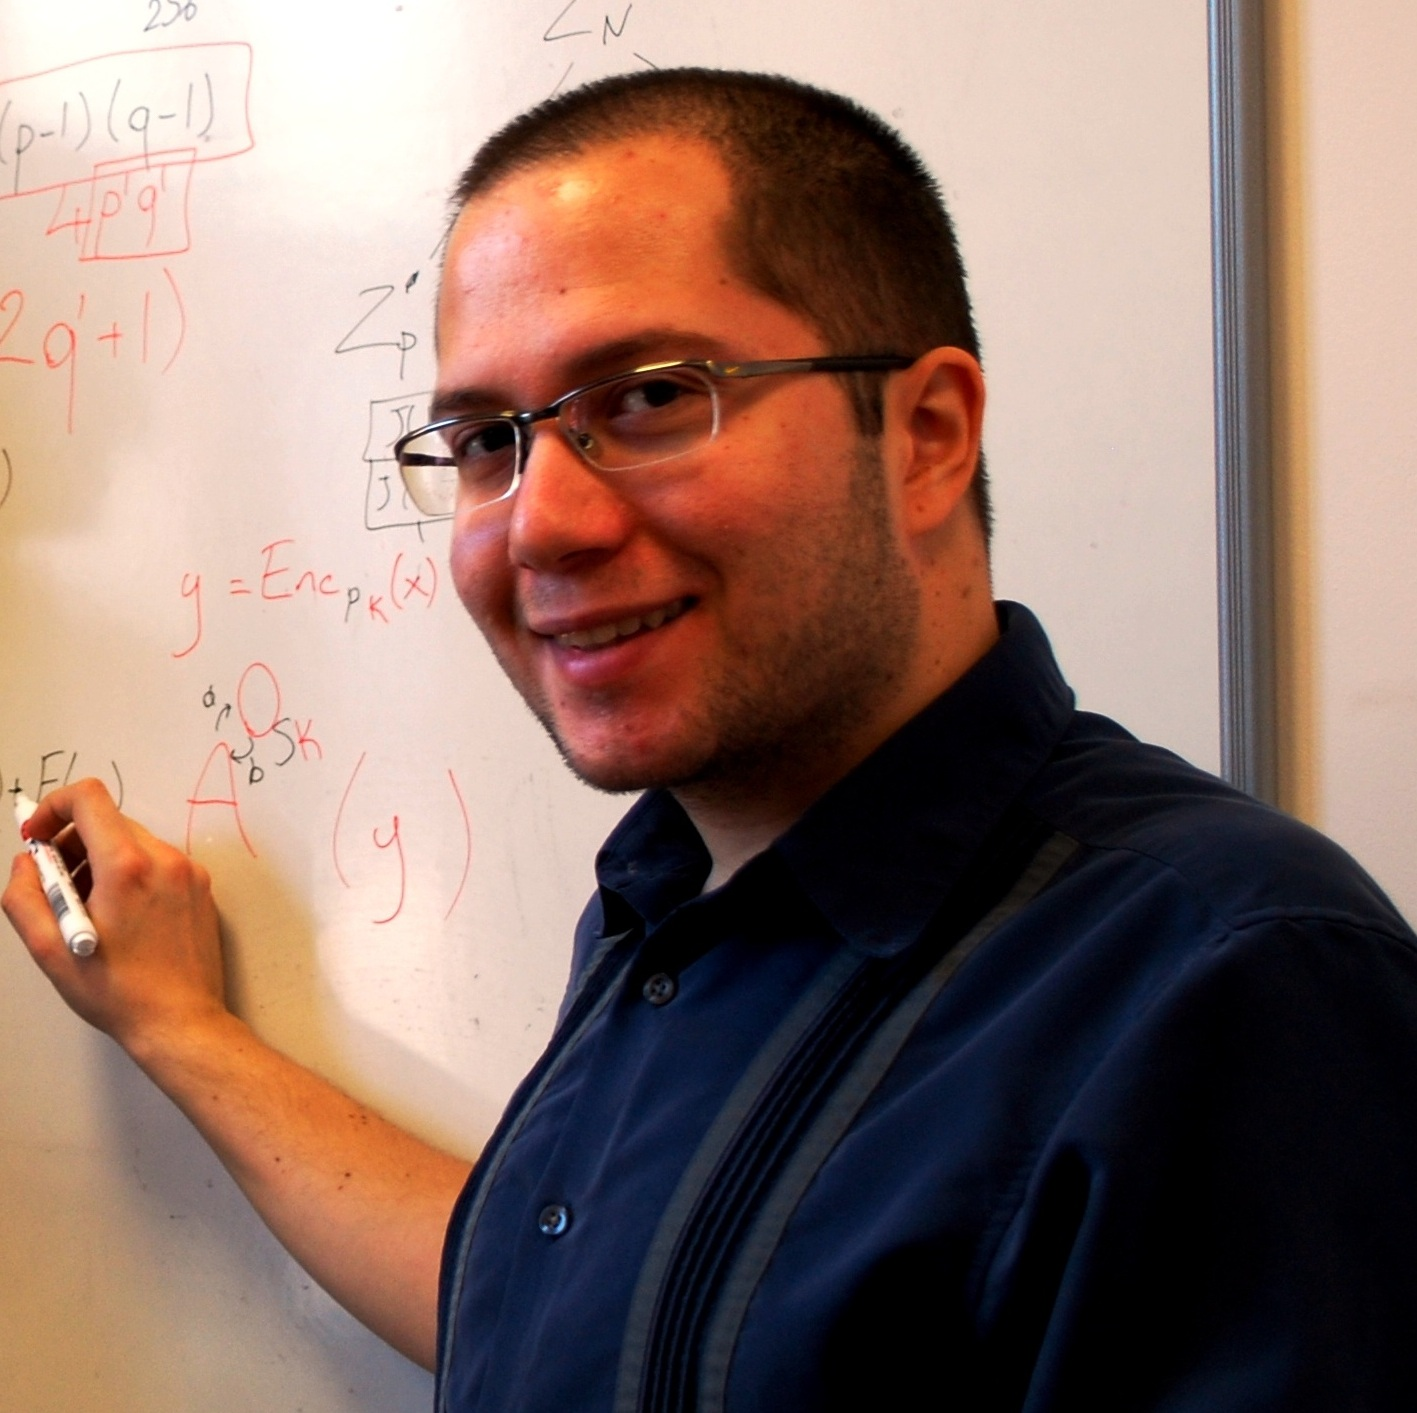
\includegraphics[width=1in,height=1.25in,clip,keepaspectratio]{authors/alptekinkupcu3.jpg}}]
{Prof. ALPTEKİN KÜPÇÜ}~received his Ph.D. degree from Brown University Computer Science Department in 2010. Since then, he has been working as a faculty member at Koç University, leading the Cryptography, Cyber Security \& Privacy Research Group that he founded. Dr. Küpçü has various accomplishments including 8 international patents granted, 16 funded research projects (for 14 of which he was the principal investigator), 2 European Union COST Action management committee memberships, 4 Outstanding Teaching Awards, 4 Outstanding Young Scientist Awards, ACM and IEEE Senior Member Awards, and the Royal Society of UK Newton Advanced Fellowship. He is also a co-founder of Xtinge Technology Inc. 
\end{IEEEbiography}

\begin{IEEEbiography}
[{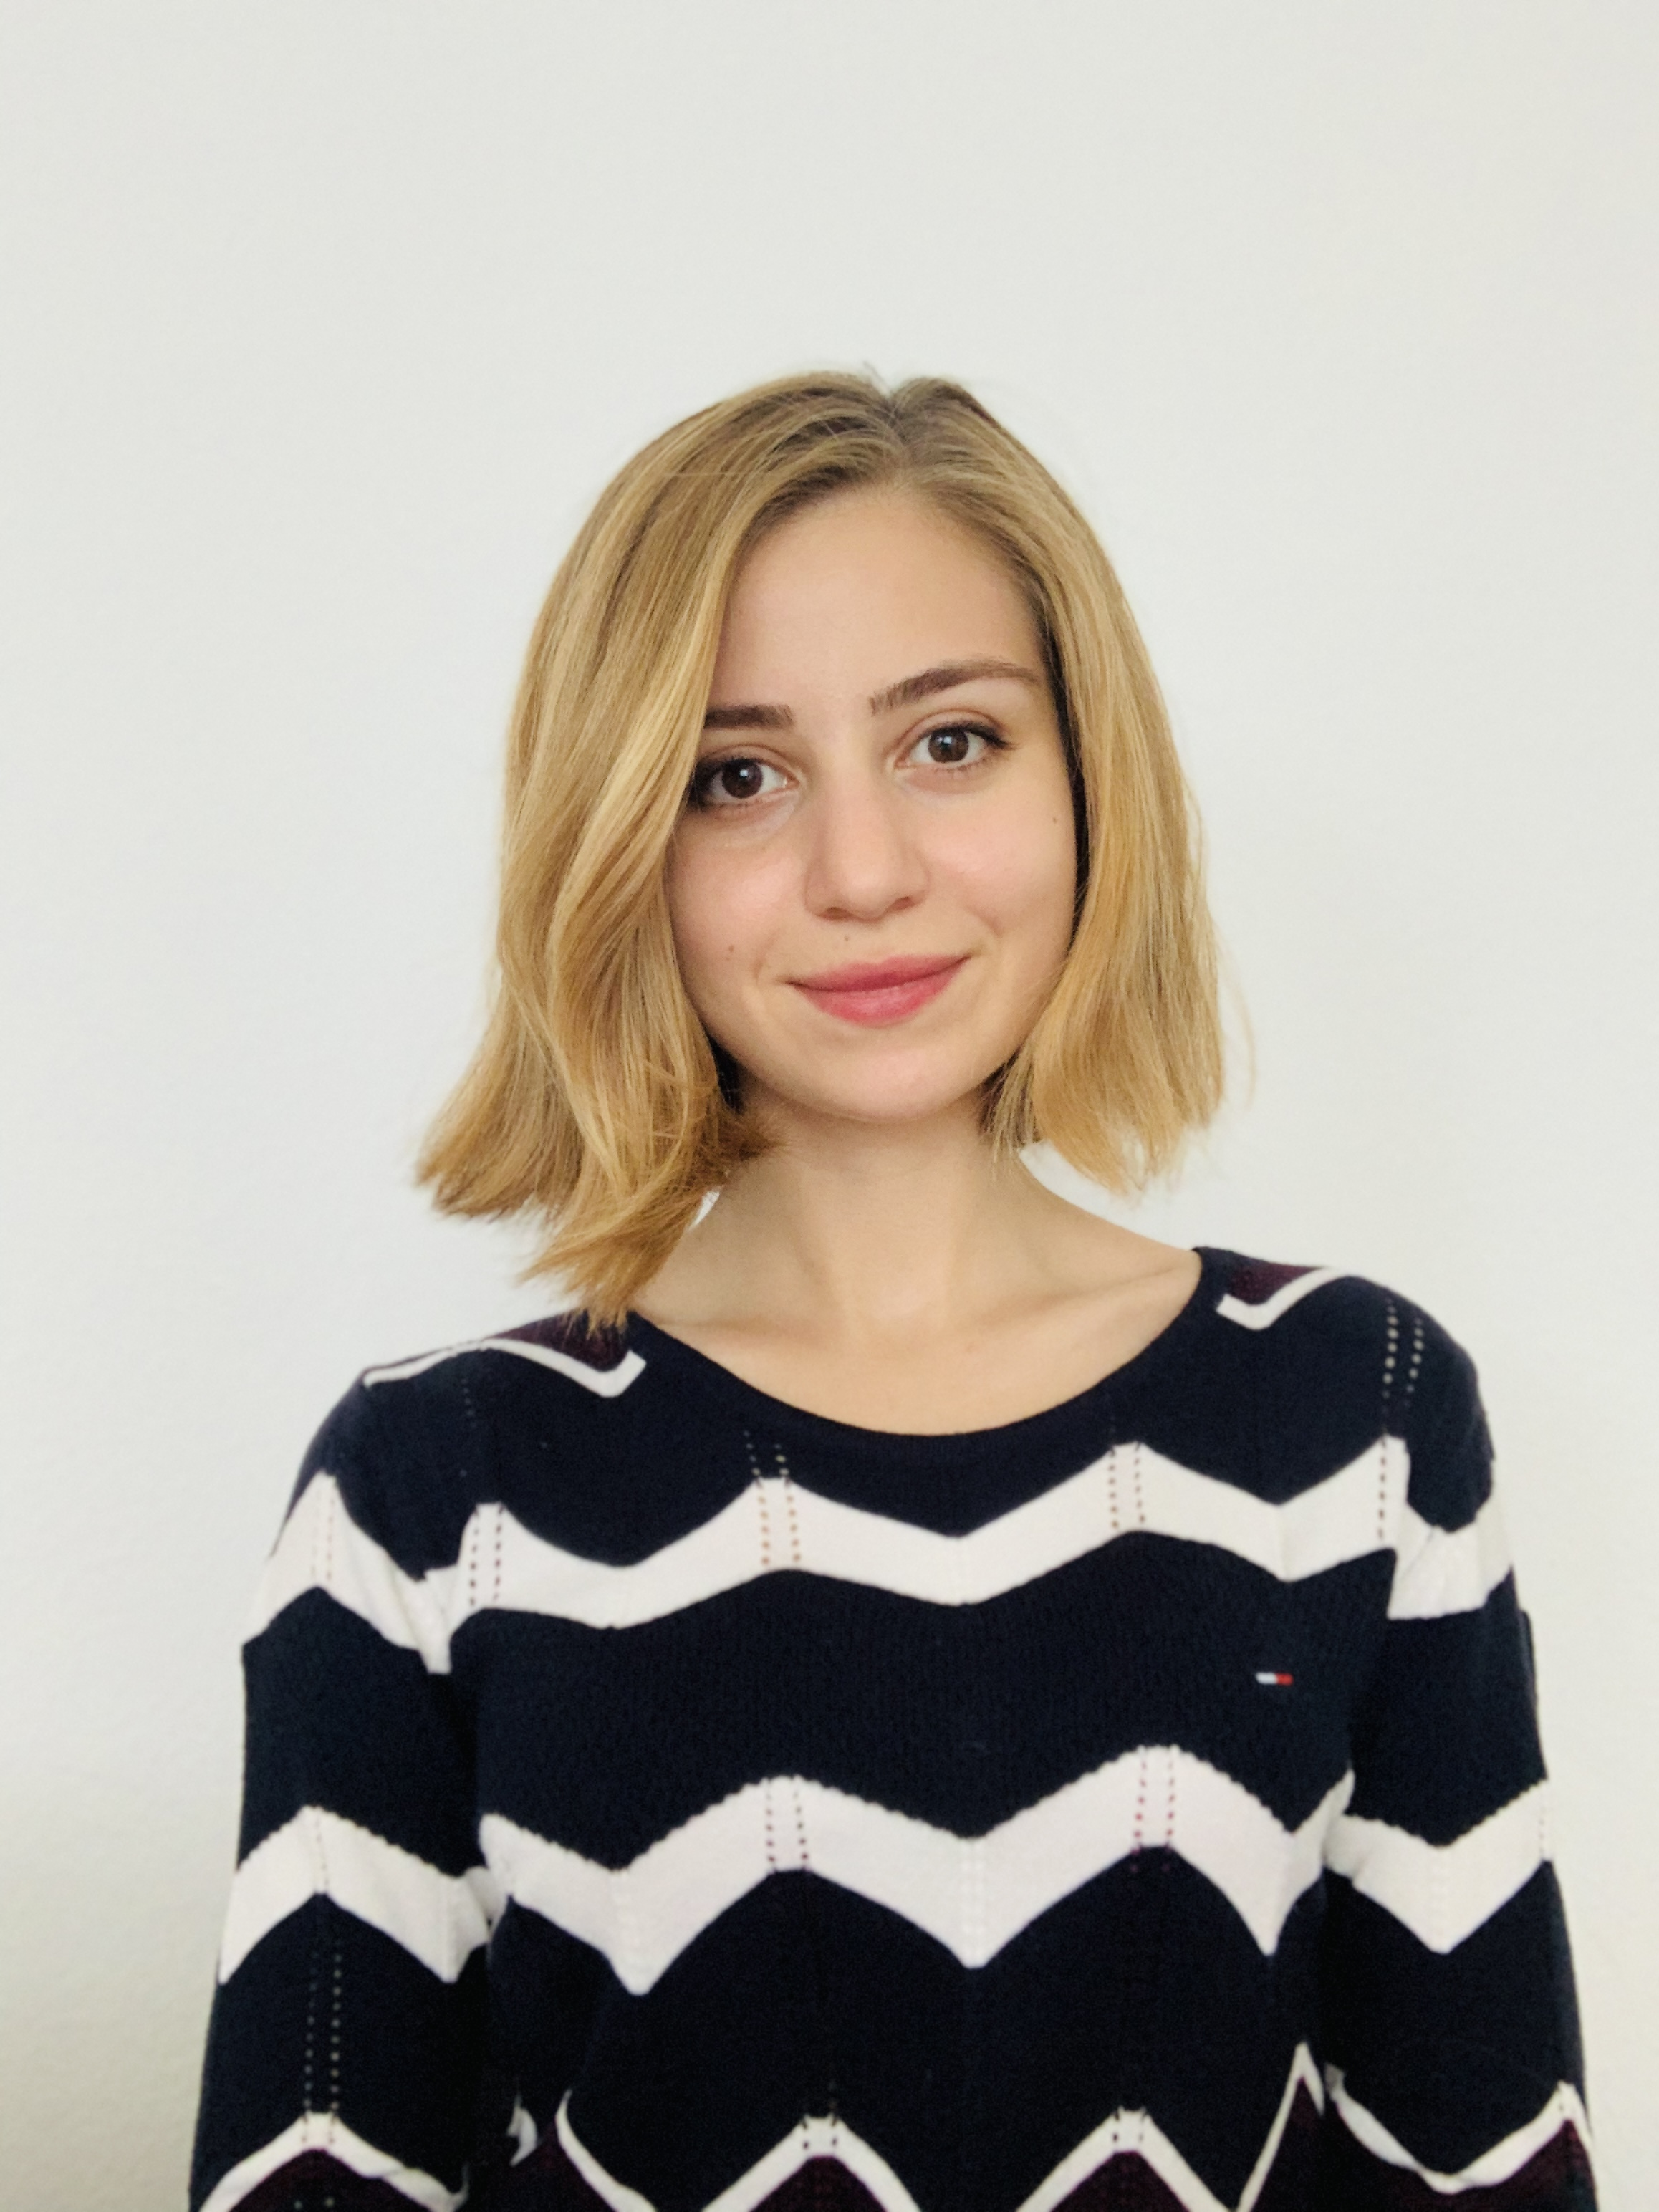
\includegraphics[width=1in,height=1.25in,clip,keepaspectratio]{authors/sinem.jpg}}]
{Asst. Prof. SİNEM SAV}~received her Ph.D. in Computer and Communication Sciences from École Polytechnique Fédérale de Lausanne (EPFL). She also holds M.Sc. and B.Sc. degrees in Computer Engineering from Bilkent University, where she currently serves as an Assistant Professor in the Computer Engineering department. Her research interests include privacy-preserving machine learning and applied cryptography. 
\end{IEEEbiography}

\end{document}



% \documentclass[lettersize,journal]{IEEEtran}
% \usepackage{amsmath,amsfonts,amssymb}
% \usepackage{algorithmic}
% \usepackage{algorithm}
% \usepackage{array}
% \usepackage[caption=false,font=normalsize,labelfont=sf,textfont=sf]{subfig}
% \usepackage{textcomp}
% \usepackage{stfloats}
% \usepackage{url}
% \usepackage{verbatim}
% \usepackage{graphicx}
% \usepackage{booktabs}
% \usepackage{multirow}
% \usepackage{makecell}
% \usepackage{enumitem}
% \usepackage{hyperref}
% \usepackage{xcolor}
% \usepackage{stmaryrd}
% \usepackage{tikz}
% \usepackage{soul}
% \usepackage{orcidlink}
% \hyphenation{op-tical net-works semi-conduc-tor IEEE-Xplore}
% \def\BibTeX{{\rm B\kern-.05em{\sc i\kern-.025em b}\kern-.08em
%     T\kern-.1667em\lower.7ex\hbox{E}\kern-.125emX}}
% \usepackage{balance}

% % Double brackets for encryption notation
% \newcommand{\enc}[1]{\llbracket #1 \rrbracket}

% % Theorem environments (IEEEtran compatible)
% \newtheorem{theorem}{Theorem}
% \newtheorem{definition}{Definition}

% \begin{document}
% \title{HE-IFD: One-Shot Federated Knowledge Distillation via Progressive Stacking under CKKS Encryption}


% % \author{
% % Halil \.{I}brahim Kanpak\,\orcidlink{0000-0000-0000-0000},
% % \IEEEauthorblockA{Ko\c{c} University}
% % \and
% % \IEEEauthorblockN{Alptekin K\"up\c{c}\"u}
% % \IEEEauthorblockA{Ko\c{c} University}
% % \and
% % \IEEEauthorblockN{Sinem Sav}
% % \IEEEauthorblockA{Bilkent University}
% % }
% % \author{
% % Erg\"un Batuhan Kaynak\,\orcidlink{0000-0002-3249-3343},
% % Kerem Bayramoglu\,\orcidlink{0009-0009-2850-9945},
% % and Sinem Sav\,\orcidlink{0000-0001-9096-8768}%

% % \thanks{All authors are with the Department of Computer Engineering, Bilkent University, Ankara, Turkey. Corresponding Author: Sinem Sav}%
% % \thanks{Ergün Batuhan Kaynak (e-mail: batuhan.kaynak@bilkent.edu.tr).}% 
% % \thanks{Kerem Bayramoglu (e-mail: kerem.bayramoglu@cs.bilkent.edu.tr).}% 
% % \thanks{Sinem Sav (e-mail: sinem.sav@cs.bilkent.edu.tr).}% 
% % \thanks{Manuscript received XX XX, XXXX; revised XX XX, XXXX.}% 
% % }

% % \author{
% % Halil \.{I}brahim Kanpak\,\orcidlink{0000-0000-0000-0000},
% % \IEEEauthorblockA{Ko\c{c} University}
% % \and
% % \IEEEauthorblockN{Alptekin K\"up\c{c}\"u\,\orcidlink{0000-0000-0000-0000}}
% % \IEEEauthorblockA{Ko\c{c} University}
% % \and
% % \IEEEauthorblockN{Sinem Sav\,\orcidlink{0000-0000-0000-0000}}
% % \IEEEauthorblockA{Bilkent University}
% % }

% \author{
% Halil \.{I}brahim Kanpak\,\orcidlink{0009-0005-0284-5941},
% Alptekin K\"up\c{c}\"u\,\orcidlink{0000-0000-0000-0000},
% and Sinem Sav\,\orcidlink{0000-0000-0000-0000}%
% \thanks{Corresponding Author: Sinem Sav}
% \thanks{Halil \.{I}brahim Kanpak is with the Department of Computer Engineering, Ko\c{c} University, Istanbul, Turkey (e-mail: hkanpak21@ku.edu.tr).}%
% \thanks{Alptekin K\"up\c{c}\"u is with the Department of Computer Engineering, Ko\c{c} University, Istanbul, Turkey (e-mail: akupcu@ku.edu.tr).}%
% \thanks{Sinem Sav is with the Department of Computer Engineering, Bilkent University, Ankara, Turkey (e-mail: sinem.sav@cs.bilkent.edu.tr).}%
% \thanks{Manuscript received XX XX, XXXX; revised XX XX, XXXX.}%
% }



% \maketitle

% \begin{abstract}

% Federated learning enables collaborative training while keeping client data local, yet sharing model updates or distillation targets, where a student model is trained to mimic a teacher's outputs, with a central server still exposes private information. Existing mitigations, such as differential privacy and secure aggregation, either degrade model quality or fail to prevent the server from inspecting the aggregated signal. Homomorphic encryption (HE) offers cryptographic protection, but an iterative training of deep networks with HE is prohibitively expensive due to large multiplicative depth.

% We present HE-IFD, a one-shot federated knowledge distillation framework in which all client contributions remain encrypted throughout server-side processing. 
% Each client trains a local teacher model and extracts intermediate feature pairs at each block boundary, where a block is a contiguous group of layers (e.g., a residual stage) whose input and output are matched during distillation. These pairs are uploaded once, encrypted under the Cheon-Kim-Kim-Song (CKKS) HE scheme, which supports approximate arithmetic over real-valued data without decryption. The server then distills these encrypted supervision signals into a full-depth HE-compatible homomorphic encryption operable student model without ever observing plaintext data, weights, or activations.
  
% Training an HE-compatible student with polynomial activations and no batch normalisation is unstable under standard end-to-end distillation. We address this with progressive stacking: block-by-block training where each block receives fresh ciphertexts, avoiding multiplicative depth accumulation across blocks. Combined with client-side collaborative normalisation, magnitude-regularised loss, and student-input training, this procedure yields stable convergence across heterogeneous multi-client settings. Under non-IID data partitions, which is the most realistic setting, the student aggregates specialised knowledge from all teachers, matching or exceeding the performance that each teacher achieves on its own local class distribution. This presents a strong participation incentive for every client, even when the student's global accuracy is lower than that of the best individual teacher. 

% % The CKKS encryption provides cryptographically guaranteed privacy against a semi-honest server, making additional defences such as differential privacy unnecessary for training-time protection.

% \end{abstract}

% \begin{IEEEkeywords}
% Federated learning, knowledge distillation, homomorphic encryption, CKKS, polynomial activation, privacy-preserving machine learning
% \end{IEEEkeywords}
% \documentclass[lettersize,journal]{IEEEtran}
% \usepackage{amsmath,amsfonts,amssymb}
% \usepackage{algorithmic}
% \usepackage{algorithm}
% \usepackage{array}
% \usepackage[caption=false,font=normalsize,labelfont=sf,textfont=sf]{subfig}
% \usepackage{textcomp}
% \usepackage{stfloats}
% \usepackage{url}
% \usepackage{verbatim}
% \usepackage{graphicx}
% \usepackage{booktabs}
% \usepackage{multirow}
% \usepackage{makecell}
% \usepackage{enumitem}
% \usepackage{hyperref}
% \usepackage{xcolor}
% \usepackage{stmaryrd}
% \usepackage{tikz}
% \usepackage{soul}
% \usepackage{orcidlink}
% \hyphenation{op-tical net-works semi-conduc-tor IEEE-Xplore}
% \def\BibTeX{{\rm B\kern-.05em{\sc i\kern-.025em b}\kern-.08em
%     T\kern-.1667em\lower.7ex\hbox{E}\kern-.125emX}}
% \usepackage{balance}

% % Double brackets for encryption notation
% \newcommand{\enc}[1]{\llbracket #1 \rrbracket}

% % Theorem environments (IEEEtran compatible)
% \newtheorem{theorem}{Theorem}
% \newtheorem{definition}{Definition}

% \begin{document}
% \title{HE-IFD: One-Shot Federated Knowledge Distillation via Progressive Stacking under CKKS Encryption}


% % \author{
% % Halil \.{I}brahim Kanpak\,\orcidlink{0000-0000-0000-0000},
% % \IEEEauthorblockA{Ko\c{c} University}
% % \and
% % \IEEEauthorblockN{Alptekin K\"up\c{c}\"u}
% % \IEEEauthorblockA{Ko\c{c} University}
% % \and
% % \IEEEauthorblockN{Sinem Sav}
% % \IEEEauthorblockA{Bilkent University}
% % }
% % \author{
% % Erg\"un Batuhan Kaynak\,\orcidlink{0000-0002-3249-3343},
% % Kerem Bayramoglu\,\orcidlink{0009-0009-2850-9945},
% % and Sinem Sav\,\orcidlink{0000-0001-9096-8768}%

% % \thanks{All authors are with the Department of Computer Engineering, Bilkent University, Ankara, Turkey. Corresponding Author: Sinem Sav}%
% % \thanks{Ergün Batuhan Kaynak (e-mail: batuhan.kaynak@bilkent.edu.tr).}% 
% % \thanks{Kerem Bayramoglu (e-mail: kerem.bayramoglu@cs.bilkent.edu.tr).}% 
% % \thanks{Sinem Sav (e-mail: sinem.sav@cs.bilkent.edu.tr).}% 
% % \thanks{Manuscript received XX XX, XXXX; revised XX XX, XXXX.}% 
% % }

% % \author{
% % Halil \.{I}brahim Kanpak\,\orcidlink{0000-0000-0000-0000},
% % \IEEEauthorblockA{Ko\c{c} University}
% % \and
% % \IEEEauthorblockN{Alptekin K\"up\c{c}\"u\,\orcidlink{0000-0000-0000-0000}}
% % \IEEEauthorblockA{Ko\c{c} University}
% % \and
% % \IEEEauthorblockN{Sinem Sav\,\orcidlink{0000-0000-0000-0000}}
% % \IEEEauthorblockA{Bilkent University}
% % }

% \author{
% Halil \.{I}brahim Kanpak\,\orcidlink{0009-0005-0284-5941},
% Alptekin K\"up\c{c}\"u\,\orcidlink{0000-0000-0000-0000},
% and Sinem Sav\,\orcidlink{0000-0000-0000-0000}%
% \thanks{Corresponding Author: Sinem Sav}
% \thanks{Halil \.{I}brahim Kanpak is with the Department of Computer Engineering, Ko\c{c} University, Istanbul, Turkey (e-mail: hkanpak21@ku.edu.tr).}%
% \thanks{Alptekin K\"up\c{c}\"u is with the Department of Computer Engineering, Ko\c{c} University, Istanbul, Turkey (e-mail: akupcu@ku.edu.tr).}%
% \thanks{Sinem Sav is with the Department of Computer Engineering, Bilkent University, Ankara, Turkey (e-mail: sinem.sav@cs.bilkent.edu.tr).}%
% \thanks{Manuscript received XX XX, XXXX; revised XX XX, XXXX.}%
% }



% \maketitle

% \begin{abstract}

% Federated learning enables collaborative training while keeping client data local, yet sharing model updates or distillation targets, where a student model is trained to mimic a teacher's outputs, with a central server still exposes private information. Existing mitigations, such as differential privacy and secure aggregation, either degrade model quality or fail to prevent the server from inspecting the aggregated signal. Homomorphic encryption (HE) offers cryptographic protection, but an iterative training of deep networks with HE is prohibitively expensive due to large multiplicative depth.

% We present HE-IFD, a one-shot federated knowledge distillation framework in which all client contributions remain encrypted throughout server-side processing. 
% Each client trains a local teacher model and extracts intermediate feature pairs at each block boundary, where a block is a contiguous group of layers (e.g., a residual stage) whose input and output are matched during distillation. These pairs are uploaded once, encrypted under the Cheon-Kim-Kim-Song (CKKS) HE scheme, which supports approximate arithmetic over real-valued data without decryption. The server then distills these encrypted supervision signals into a full-depth HE-compatible homomorphic encryption operable student model without ever observing plaintext data, weights, or activations.
  
% Training an HE-compatible student with polynomial activations and no batch normalisation is unstable under standard end-to-end distillation. We address this with progressive stacking: block-by-block training where each block receives fresh ciphertexts, avoiding multiplicative depth accumulation across blocks. Combined with client-side collaborative normalisation, magnitude-regularised loss, and student-input training, this procedure yields stable convergence across heterogeneous multi-client settings. Under non-IID data partitions, which is the most realistic setting, the student aggregates specialised knowledge from all teachers, matching or exceeding the performance that each teacher achieves on its own local class distribution. This presents a strong participation incentive for every client, even when the student's global accuracy is lower than that of the best individual teacher. 

% % The CKKS encryption provides cryptographically guaranteed privacy against a semi-honest server, making additional defences such as differential privacy unnecessary for training-time protection.

% \end{abstract}

% \begin{IEEEkeywords}
% Federated learning, knowledge distillation, homomorphic encryption, CKKS, polynomial activation, privacy-preserving machine learning
% \end{IEEEkeywords}



% \section{INTRODUCTION}
\label{sec:introduction}

Federated Learning (FL) prevents raw data sharing among clients, but joint model training can still leak information through repeated gradient exchange~\cite{zhu2019deep, so2023securing}. One-shot FL reduces communication overhead and privacy exposure by limiting communication to a single round, where intermediate gradient exchanges are not performed. However, if the transferred distillation targets are visible to the server in plaintext, the privacy risk remains~\cite{jagielski2023students}.

Differential Privacy (DP) and secure aggregation partially address this risk, with their own limitations. Strong DP noise degrades distillation quality~\cite{shao2023selective}, while secure aggregation protects individual values without preventing the server from inspecting the aggregate~\cite{kerkouche2023client}. Homomorphic encryption (HE) provides end-to-end cryptographic protection; yet direct iterative HE training of deep models is prohibitively expensive due to multiplicative depth constraints~\cite{zhang2020batchcrypt, jin2023fedml, kanpak2024cure}. This motivates a distillation-based design that is both one-shot and HE-compatible. The main technical challenge is that HE computation supports only addition and multiplication over ciphertexts, whereas standard neural network operations, e.g., ReLU, batch normalisation, softmax, are non-polynomial. Recent work addresses the stability of polynomial activations for HE-compatible networks by deriving tighter ReLU approximations~\cite{agamennone2025polynomial} and proposing boundary-loss and gradient-clipping strategies for deep polynomial training~\cite{alhossain2025training}. However, these methods target centralised inference or single-model training. Stable and efficient training of deep polynomial student models under encrypted federated supervision, where heterogeneous clients produce targets with incompatible magnitude distributions, remains an open problem.

% Also, while existing work on one-shot HE distillation focuses on encrypted inference~\cite{agamennone2025polynomial, alhossain2025training}, training deep student models efficiently under encryption remains an open problem.


For this reason, we focus on one-shot federated knowledge distillation under homomorphic encryption. In knowledge distillation, a compact \emph{student} model learns by imitating the internal representations of a stronger pre-trained \emph{teacher}, rather than training directly on labelled data. In our setting, each client acts as a teacher by training a local model on its private data and contributing encrypted supervision signals derived from that model in a single communication round. The server then uses these signals to train a privacy-preserving student entirely on ciphertexts, without ever accessing any plaintext data, weights, or activations.

% For this reason, we focus on one-shot federated knowledge distillation under homomorphic encryption: clients contribute encrypted teacher supervision in a single round, and the server trains a privacy-preserving student model entirely on ciphertexts, without ever accessing any plaintext data, weights, or activations.

\subsection{Motivation}
\label{sec:intro_motivation}

One-shot federated learning~\cite{guha2019oneshot, wang2025towards} limits client--server communication to a single round, eliminating the iterative exposure that facilitates multi-round attacks. Knowledge distillation suits this setting naturally: clients train local teachers and transfer knowledge to a server-side student in a single step. However, data heterogeneity causes inconsistent teacher logits, and as shown in Section~\ref{sec:bg_server_inference}, even this single round of plaintext transfer remains exploitable by the server. Encrypting the transferred knowledge is therefore necessary, not optional.

Homomorphic encryption (HE)~\cite{cheon2017ckks} provides end-to-end cryptographic protection without injecting noise, avoiding the utility--privacy tradeoff of DP. However, applying HE to standard iterative training is structurally expensive. The systems reviewed in Section~\ref{sec:bg_he_fl} (POSEIDON, BatchCrypt, FedSHE) all encrypt per-round gradient updates and therefore exhaust the multiplicative-depth budget of CKKS~\cite{cheon2017ckks} (further discussed in Section~\ref{sec:ckks_prelim}) in every round; bootstrapping~\cite{cheon2018bootstrapping} refreshes the budget but at substantial latency. One-shot settings resolve this tension: ciphertexts are used once, and block-independent training with fresh ciphertexts confines the depth budget to a single block of the student rather than the full network. This principle was recently validated for encrypted MLP training~\cite{pirillo2025reboot}. HE-IFD extends it to federated one-shot distillation over heterogeneous clients.

DP partially addresses plaintext leakage but degrades the distillation signal. Applying local DP causes severe accuracy drops (up to $70\%$ on CIFAR-100 at $\epsilon = 0.1$~\cite{gad2024communication}), and one-shot settings consume the entire privacy budget immediately, precluding amplification across rounds. At meaningful privacy levels ($\epsilon \leq 1$), DP reduces FedMD to near random-guessing accuracy~\cite{sun2021fedmdnfdp}. HE avoids this tradeoff entirely.

\subsection{Our Approach}
We present \textbf{HE-IFD} (\textbf{H}omomorphic \textbf{E}ncryption-\textbf{I}ntermediate \textbf{F}eature \textbf{D}istillation), a framework in which individual client teacher outputs are protected during knowledge transfer and all subsequent server-side computation. The protocol operates in three phases:

\begin{enumerate}
\item \textbf{Local training.} Each client trains a standard teacher model (e.g., ResNet-18) on their private data partition, starting from a shared random initialisation.
\item \textbf{Encrypted upload.} Each client runs its teacher model on its own data and records the inputs and outputs at each layer group boundary. We refer to these groups as \emph{blocks}. These input--output pairs tell the server what each block of the teacher produces, without revealing the raw data. Before encrypting, clients jointly agree on per-channel normalisation statistics so that features from different clients are on a comparable scale. The normalised pairs are then encrypted under Cheon--Kim--Kim--Song (CKKS) scheme and uploaded to the server in a single round; no further client interaction is needed.
\item \textbf{Server-side encrypted distillation.} The server trains a HE-compatible architecture in which non-polynomial operations such as ReLU and batch normalisation are replaced with polynomial equivalents that can be evaluated directly on ciphertexts (e.g., PolyResNet-18) for the student model on the server, block by block, using only encrypted inputs and targets. Student weights, activations, gradients, and loss values are all ciphertext throughout training.
\end{enumerate}

The server never observes any individual teacher output, student weight, or intermediate activation in plaintext. It operates as a blind compute delegate that executes the distillation protocol on encrypted data. Four properties of the protocol class determine the design and govern what can be proven about it; each is the structural answer to a distinct concern raised by the rejected version's review cycle.

\par\noindent\textbf{(C1) HE depth budget for an end-to-end encrypted student update.} A naive encrypted SGD step that forward-propagates through encrypted weights accumulates one multiplicative level per affine layer plus the degree of every polynomial activation, which exceeds the level chain available in any practical CKKS parameterisation long before the student converges. We avoid the naive construction. The encrypted state at every step is a \emph{linear accumulator} over teacher-induced gradient contributions, $\langle\theta_E\rangle = \langle\theta_0^\star\rangle + \sum_t \eta\,\langle g_t\rangle$, where each $\langle g_t\rangle$ is computed from the encrypted teacher signal applied to a plaintext student state. The per-step depth is at most three multiplicative levels (residual carry-over, scalar-by-ciphertext for the learning rate, addition to the accumulator), and the dominant ciphertext-by-ciphertext cost is confined to the depth-3 ensemble target construction described in Section~\ref{sec:phase2}; the full protocol fits inside a single CKKS level chain at $\log N \in \{14, 15\}$ with no bootstrapping. The structural justification for the plaintext student state during training, and for what is and is not allowed to be threshold-decrypted, is the binding invariant developed in Section~\ref{sec:threat_binding}.

\par\noindent\textbf{(C2) $\beta/\lambda$ ensemble boost without division under HE.} Pooling per-client encrypted teacher logits into an ensemble target with confidence-aware reweighting requires both a per-client confidence weight $\alpha_i^\beta$ and a per-row data-boost factor $1+\lambda V_k$ on the encrypted variance across teachers. Both knobs are constructed in CKKS without any encrypted division: the $\beta$-power is taken on the plaintext scalar $\alpha_i$ and applied as a scalar-by-ciphertext multiplication, and the per-row variance is built as $\langle V_k\rangle = \sum_i w_i \langle T_{i,k}\rangle^2 - \langle\bar T_k\rangle^2$ at depth 1. The resulting ensemble target is at most three multiplicative levels deep regardless of $N$. The construction is detailed in Section~\ref{sec:phase2}; the same section formalises why the depth bound is independent of $N$ and why a per-class coverage-aware variant of $\beta$ is the natural extension at the lowest-$\alpha$ heterogeneity settings.

\par\noindent\textbf{(C3) Binding invariant under $N{-}1$ collusion.} The cryptographic primitive is the multiparty variant of CKKS in the threshold instantiation at $t{=}N$: all $N$ secret-key shares must concur to recover any plaintext. The choice $t{=}N$ rather than $t < N$ is deliberate, because any $t < N$ admits a coalition of $t{-}1$ semi-honest clients who can decrypt the per-client logit ciphertexts and the aggregated ensemble target, which under the present threat model directly enables subtraction attacks against the remaining honest client. The protocol's central security property, that the only ciphertext ever subjected to threshold decryption is the final trained student $\theta_E$, is the binding invariant, formalised in Section~\ref{sec:threat_binding}. With the invariant, the adversary's view (server in coalition with up to $N{-}1$ clients) consists of IND-CPA ciphertexts, plaintext metadata (probe set, ciphertext sizes, timing), and the released student alone.

\par\noindent\textbf{(C4) Post-release statistical-query-floor mitigation.} The binding invariant prevents direct decryption attacks on intermediate state, but it does not rule out a derived form, utility-coercion-into-privacy-amplification: if $N{-}1$ colluding clients upload all-zero logit ciphertexts, the encrypted ensemble target collapses to a multiple of the single honest client's logits and the released student becomes a single-teacher distillation of that honest teacher. The attack does not breach the invariant; it inflates the unavoidable statistical-query floor on $\theta_E$. The protocol admits two independent defensive knobs: each client trains its teacher with DP-SGD at a per-client budget $(\varepsilon_T, \delta_T)$ that survives by post-processing into the released student, and each client may add per-row Gaussian noise to its logit vector before encryption, which surfaces at full magnitude under the all-zeros amplification and averages to $\sigma_P/\sqrt N$ in the honest case. The composition is bounded by the standard Gaussian-DP RDP accountant. The construction is developed in Section~\ref{sec:threat_binding}.

Together, these four properties (the depth budget for the linear accumulator, the division-free $\beta/\lambda$ ensemble boost, the binding invariant on threshold decryption, and the SQ-floor mitigation by DP-SGD teachers plus per-row Gaussian noise) determine the design of the protocol. Section~\ref{sec:methodology} develops each of them; Section~\ref{sec:experiments} reports the resulting accuracy on MNIST and CIFAR-10 against the strongest published one-shot baselines, and shows that the encrypted student consistently exceeds the mean individual teacher accuracy across heterogeneity settings, with the largest margins at the smallest $\alpha$.


% A key technical difficulty is training an HE-compatible student, which uses polynomial activations and HE-compatible normalisation layers instead of ReLU and batch normalisation, from encrypted supervision. Standard end-to-end distillation diverges for this architecture. We solve this with training the model sequentially, one block at a time, where each block is an independent sub-network spanning a few layers, with each block receiving fresh ciphertexts, combined with magnitude-regularised normalised MSE loss and student-input training. This approach yields stable convergence and competitive accuracy across our CIFAR-10 and Fashion-MNIST experiments.


\subsection{Contributions}
Our contributions are as follows:

\begin{enumerate}
\item We propose, for the first time, progressive stacking for training HE-compatible student models fully under encryption: a block-by-block procedure with magnitude-regularised normalised MSE loss that achieves stable distillation of a full PolyResNet-18 student (11.17M parameters) from encrypted teacher features, where standard end-to-end distillation diverges.

\item We present a novel, fully encrypted one-shot distillation protocol in which clients upload encrypted per-block feature pairs in a single communication round and the server performs all distillation computation (forward pass, loss evaluation, backward pass, and weight update) entirely on ciphertexts, without exposing any plaintext data at any point during training.

\item We introduce client-side collaborative normalisation, a lightweight technique in which each client normalises its teacher outputs to zero mean and unit variance per channel before encryption, which eliminates magnitude incompatibility across heterogeneous teachers and prevents training divergence for $N \geq 4$ clients.

\item We provide a comprehensive empirical evaluation of HE-IFD across three architectures (ResNet-18, SimpleCNN, ViT-B/32), client counts $N \in \{1, 2, 4, 8, 16, 32\}$, and heterogeneity levels $\alpha \in \{0.1, 1.0\}$, including accuracy comparisons against differential privacy baselines, membership inference attack analysis, and communication and computation cost analysis.
\end{enumerate}

%The remainder of this paper is organized as follows. Section~\ref{sec:background} surveys federated learning, knowledge distillation, privacy mechanisms, and homomorphic encryption. Section~\ref{sec:methodology} presents the HE-IFD framework. Section~\ref{sec:experiments} reports experimental results. Section~\ref{sec:conclusion} concludes.

    

% \section{INTRODUCTION}
% \label{sec:introduction}

% Federated Learning (FL) prevents raw data sharing among clients, but joint model training can still leak information through repeated gradient exchange~\cite{zhu2019deep, so2023securing}. One-shot FL reduces communication overhead and privacy exposure by limiting communication to a single round, where intermediate gradient exchanges are not performed. However, if the transferred distillation targets are visible to the server in plaintext, the privacy risk remains~\cite{jagielski2023students}.

% Differential Privacy (DP) and secure aggregation partially address this risk, with their own limitations. Strong DP noise degrades distillation quality~\cite{shao2023selective}, while secure aggregation protects individual values without preventing the server from inspecting the aggregate~\cite{kerkouche2023client}. Homomorphic encryption (HE) provides end-to-end cryptographic protection; yet direct iterative HE training of deep models is prohibitively expensive due to multiplicative depth constraints~\cite{zhang2020batchcrypt, jin2023fedml, kanpak2024cure}. This motivates a distillation-based design that is both one-shot and HE-compatible. The main technical challenge is that HE computation supports only addition and multiplication over ciphertexts, whereas standard neural network operations, e.g., ReLU, batch normalisation, softmax, are non-polynomial. Recent work addresses the stability of polynomial activations for HE-compatible networks---deriving tighter ReLU approximations~\cite{agamennone2025polynomial} and proposing boundary-loss and gradient-clipping strategies for deep polynomial training~\cite{alhossain2025training}, but these methods target centralised inference or single-model training. Stable and efficient training of deep polynomial student models under encrypted federated supervision, where heterogeneous clients produce targets with incompatible magnitude distributions, remains an open problem.

% % Also, while existing work on one-shot HE distillation focuses on encrypted inference~\cite{agamennone2025polynomial, alhossain2025training}, training deep student models efficiently under encryption remains an open problem.




% For this reason, we focus on one-shot federated knowledge distillation under homomorphic encryption. In knowledge distillation, a compact \emph{student} model learns by imitating the internal representations of a stronger pre-trained \emph{teacher}, rather than training directly on labelled data. In our setting, each client acts as a teacher by training a local model on its private data and contributing encrypted supervision signals derived from that model in a single communication round. The server then uses these signals to train a privacy-preserving student entirely on ciphertexts, without ever accessing any plaintext data, weights, or activations.

% % For this reason, we focus on one-shot federated knowledge distillation under homomorphic encryption: clients contribute encrypted teacher supervision in a single round, and the server trains a privacy-preserving student model entirely on ciphertexts, without ever accessing any plaintext data, weights, or activations.

% \subsection{Our Approach}
% We present \textbf{HE-IFD} (\textbf{H}omomorphic \textbf{E}ncryption-\textbf{I}ntermediate \textbf{F}eature \textbf{D}istillation), a framework in which individual client teacher outputs are protected during knowledge transfer and all subsequent server-side computation. The protocol operates in three phases:

% \begin{enumerate}
% \item \textbf{Local training.} Each client trains a standard teacher model (e.g., ResNet-18) on their private data partition, starting from a shared random initialisation.
% \item \textbf{Encrypted upload.} Each client runs its teacher model on its own data and records the inputs and outputs at each layer group boundary — we call these groups \emph{blocks}. These input--output pairs tell the server what each block of the teacher produces, without revealing the raw data. Before encrypting, clients jointly agree on per-channel normalisation statistics so that features from different clients are on a comparable scale. The normalised pairs are then encrypted under CKKS and uploaded to the server in a single round; no further client interaction is needed.
% \item \textbf{Server-side encrypted distillation.} The server trains a HE-compatible architecture in which non-polynomial operations such as ReLU and batch normalisation are replaced with polynomial equivalents that can be evaluated directly on ciphertexts (e.g., PolyResNet-18) in the student model in server, block by block, using only encrypted inputs and targets. Student weights, activations, gradients, and loss values are all ciphertext throughout training.
% \end{enumerate}

% The server never observes any individual teacher output, student weight, or intermediate activation in plaintext. It operates as a blind compute delegate that executes the distillation protocol on encrypted data.

% A key technical difficulty is training an HE-compatible student — which replaces ReLU with learnable degree-2 polynomial activations and batch normalisation with static per-channel affine layers — from encrypted intermediate supervision. Several compounding challenges make standard distillation approaches fail.

% \par\noindent\textbf{Polynomial magnitude explosion.} The quadratic activation $ax^2 + bx$ amplifies feature magnitudes at every composition. An input of magnitude 5 produces roughly 11 after one block, 44 after two; across five blocks this can reach $10^4$, causing gradient overflow. The problem is exacerbated in the multi-client setting, where teachers trained on heterogeneous data partitions produce features with incompatible magnitude ranges, and the HE-compatible replacement for batch normalisation — a static per-channel scale-and-shift — cannot dynamically compensate.

% \par\noindent\textbf{Training--distillation distribution gap.} Distilling block by block avoids CKKS depth accumulation, but training block $k$ on teacher-produced inputs creates a mismatch: at inference, block $k$ receives student-produced inputs from the frozen prefix. Without correction this collapses the composed model toward random accuracy. We address this through trainable per-channel affine bridges, initialised from uploaded feature statistics, followed by server-side sequential refinement that exposes each block to its actual inference-time distribution — without any additional client communication.

% \par\noindent\textbf{Scale-anchored distillation loss.} Standard MSE is sensitive to the sign asymmetry between polynomial activations and ReLU features and allows unbounded magnitude drift that amplifies through frozen downstream blocks. Our loss combines channel-normalised MSE, which aligns feature \textit{shape} independently of scale, with a log-ratio penalty $(\log,\sigma_{\hat{f}}/\sigma_{\tilde{f}})^2$ that anchors the student's feature \textit{magnitude} to the teacher's. Unlike a plain $\ell_2$ scale penalty, the log-ratio form penalises multiplicative over- and under-scaling symmetrically and is scale-free.

% Together these mechanisms yield stable convergence and competitive accuracy across our CIFAR-10 and Fashion-MNIST experiments under non-IID federated partitioning.

% % A key technical difficulty is training an HE-compatible student, which uses polynomial activations and HE-compatible normalisation layers instead of ReLU and batch normalisation, from encrypted supervision. Standard end-to-end distillation diverges for this architecture. We solve this with training the model sequentially, one block at a time, where each block is an independent sub-network spanning a few layers, with each block receiving fresh ciphertexts, combined with magnitude-regularised normalised MSE loss and student-input training. This approach yields stable convergence and competitive accuracy across our CIFAR-10 and Fashion-MNIST experiments.


% \subsection{Contributions}
% Our contributions are as follows:

% \begin{enumerate}
% \item We propose, for the first time, progressive stacking for training HE-compatible student models fully under encryption: a block-by-block procedure with magnitude-regularised normalised MSE loss that achieves stable distillation of a full PolyResNet-18 student (11.17M parameters) from encrypted teacher features, where standard end-to-end distillation diverges.

% \item We present a novel fully encrypted one-shot distillation protocol in which clients upload encrypted per-block feature pairs in a single communication round and the server performs all distillation computation (forward pass, loss evaluation, backward pass, and weight update) entirely on ciphertexts, without exposing any plaintext data at any point during training.

% \item We introduce client-side collaborative normalisation, a lightweight technique in which each client normalises its teacher outputs to zero mean and unit variance per channel before encryption, which eliminates magnitude incompatibility across heterogeneous teachers and prevents training divergence for $N \geq 4$ clients.

% \item We provide a comprehensive empirical evaluation of HE-IFD across client counts ($N \in \{1, 2, 4, 8, 16\}$) and heterogeneity levels ($\alpha \in \{0.1, 0.5, 1.0, 100.0\}$), reporting accuracy, a privacy analysis against membership inference attacks, and a comparison with differential privacy baselines.
% \end{enumerate}

% %The remainder of this paper is organized as follows. Section~\ref{sec:background} surveys federated learning, knowledge distillation, privacy mechanisms, and homomorphic encryption. Section~\ref{sec:methodology} presents the HE-IFD framework. Section~\ref{sec:experiments} reports experimental results. Section~\ref{sec:conclusion} concludes.



% \section{RELATED WORK AND MOTIVATION}
\label{sec:background}

%This section reviews the privacy risks of federated learning, the limitations of existing defences, and the technical constraints that motivate our design.


%% ─────────────────────────────────────────────────────
\subsection{Privacy Risks of Multi-Round Federated Learning}
\label{sec:bg_multiround}

Federated learning (FL)~\cite{mcmahan2017communication} retains raw data locally but repeatedly transmits model updates with each round, presenting an attack surface. Shared gradients can be inverted to reconstruct training images~\cite{zhu2019deep}, with recent attacks achieving exact reconstruction for batches up to $b \lesssim 25$ by exploiting ReLU-induced gradient sparsity~\cite{dimitrov2024spear}. Active and passive membership inference attacks exploit intermediate parameter updates~\cite{nasr2019comprehensive}, and GAN-based attacks reconstruct training data by exploiting evolving model dynamics across rounds~\cite{hitaj2017deep}. Even with secure aggregation, information accumulates: standard random user selection can leak individual user models within $O(N)$ rounds~\cite{so2023securing} N being the number of clients, and client-specific properties can be recovered from aggregated updates~\cite{kerkouche2023property}. Consequently, repeated communication is inherently risky regardless of raw data sharing policies~\cite{carletti2025sok}. HE-IFD eliminates this attack surface by restricting communication to a single encrypted round.


%% ─────────────────────────────────────────────────────
\subsection{Privacy Risks of Federated Distillation}
\label{sec:bg_server_inference}

Federated distillation is a class of FL methods in which clients train local teacher models and transfer knowledge to a server-side student by sharing model outputs such as
logits, soft labels, or intermediate features, rather than gradients. Several protocols utilize this paradigm: FedMD~\cite{li2019fedmd} and DS-FL~\cite{itahara2021dsfl} have clients share softmax predictions on a shared public dataset, FedDF~\cite{lin2020feddf} distils an ensemble of heterogeneous client models into a single server model, and Cronus~\cite{chang2019cronus} adds robust aggregation via spectral filtering of client predictions. However, plaintext logits and features leak private information even without gradient access, posing a central risk to unencrypted federated distillation. Model confidence values inherently provide sufficient information for inversion attacks, enabling adversaries to reconstruct training data features directly~\cite{fredrikson2015model}.

Against FedMD-style distillation, the Paired-Logits Inversion attack~\cite{takahashi2023breaching} allows a malicious server to recover high-fidelity private images by exploiting the confidence gap between its predictions and those of the clients. Even without reconstructing individual samples, an honest-but-curious server can infer a client's label distribution solely from aggregated predictions~\cite{gu2023ldia, shi2025unveiling}.

% Against FedMD-style distillation, the Paired-Logits Inversion attack~\cite{takahashi2023breaching} allows a malicious server to recover high-fidelity private images by exploiting the confidence gap between its predictions and those of the clients. Shi et al.~\cite{shi2025unveiling} demonstrate that client logit vectors encode the memorization of private data, enabling highly accurate label distribution and membership inference attacks against FedMD~\cite{li2019fedmd}, DS-FL~\cite{itahara2021dsfl}, and Cronus~\cite{chang2019cronus}. Additionally, an honest-but-curious server can infer a client's label distribution solely from aggregated predictions without reconstructing individual samples~\cite{gu2023ldia}.

Membership inference attacks pose a distinct threat by revealing whether a specific sample was used for training. FD-Leaks~\cite{yang2023fdleaks} uses a malicious client's local model as a shadow model, while GradDiff and GradDrift~\cite{wang2024graddiff} enable gradient-based inference by both servers and clients. More recent likelihood-ratio methods achieve stronger results: Co-operative LiRA and distillation-based LiRA variants~\cite{shi2025unveiling} attain high true-positive rates at low false-positive rates against FedMD and DS-FL. Distillation itself amplifies these vulnerabilities. As an example, students can exhibit up to $+9.81\%$ higher MIA susceptibility than their teachers~\cite{cui2025mia}, and the GLiRA framework~\cite{galichin2025glira} shows that knowledge-distillation-based shadow models improve likelihood-ratio attacks over the original LiRA baseline~\cite{carlini2022membership}. Even transmitting hard labels instead of soft labels only mitigates rather than eliminates this risk, as discrete predictions still leak label distributions~\cite{shao2024selective}.

% Membership inference attacks (MIA) further exacerbate these risks. FD-Leaks~\cite{yang2023fdleaks} uses a malicious client's local model as a shadow model, while GradDiff and GradDrift~\cite{wang2024graddiff} enable gradient-based inference by servers and clients. Distillation amplifies these vulnerabilities: students can exhibit up to $+9.81\%$ higher MIA susceptibility than their teachers~\cite{cui2025mia}, and the GLiRA framework~\cite{galichin2025glira} demonstrates that knowledge-distillation-based shadow models improve likelihood-ratio attacks over the original LiRA baseline~\cite{carlini2022membership}. Co-operative LiRA and distillation-based LiRA variants~\cite{shi2025unveiling} achieve high true-positive rates at low false-positive rates against FedMD- and DS-FL-style protocols. Even transmitting hard labels instead of soft labels only mitigates, rather than eliminates, this risk; discrete predictions still leak label distributions~\cite{shao2024selective}.

% \textbf{Beyond privacy: poisoning and model stealing.} 
% The attack surface extends beyond privacy violations. Logit poisoning attacks~\cite{tang2024logits} allow adversaries to manipulate shared predictions and corrupt the distilled student model. A semi-honest server can reconstruct client models from observed logits~\cite{wan2024privacy}, enabling model stealing. Even parametric feature sharing is unsafe: feature inversion can recover private images with SSIM values approaching $0.997$~\cite{beitollahi2024parametric}.

This diverse attack landscape demonstrates that plaintext knowledge transfer is fundamentally unsafe regardless of format. Only cryptographic protection eliminates these attack vectors entirely without degrading the distillation signal. HE-IFD encrypts all transferred knowledge under CKKS before upload, ensuring that the server never observes any plaintext supervision signal.



%% ─────────────────────────────────────────────────────
\subsection{One-Shot Federated Distillation}
\label{sec:bg_oneshot}

One-shot federated learning~\cite{guha2019oneshot, wang2025towards} restricts client-server communication to a single round and is the family of FL designs that share our problem statement. Among the plaintext distillation systems in this family, FedMD~\cite{li2019fedmd} and DS-FL~\cite{itahara2021dsfl} have clients transfer softmax predictions on a shared public dataset; FedDF~\cite{lin2020feddf} distils an ensemble of heterogeneous client models into a server model; Cronus~\cite{chang2019cronus} adds robust aggregation by spectrally filtering the client predictions; DENSE~\cite{zhang2022dense} uploads full plaintext models and trains a generator on the server; Co-Boosting~\cite{dai2024coboosting} iteratively co-trains data and ensemble; and FuseFL~\cite{tang2024fusefl} is architecturally closest to HE-IFD in that it also decomposes the student into blocks and trains them sequentially. None of these methods provide cryptographic protection: every client contribution reaches the server in plaintext and is therefore subject to the inversion, label-distribution, and membership-inference attacks reviewed in Section~\ref{sec:bg_server_inference}. The distinguishing axis of HE-IFD relative to this family is privacy: the supervision signal is a ciphertext under collectively held keys, and the server's view is computationally indistinguishable from random regardless of the architectural similarity to FuseFL.

The smaller subset of one-shot FL systems that do offer formal privacy guarantees rely uniformly on differential privacy. FedKT~\cite{li2021fedkt} achieves $(\varepsilon, 0)$-DP through noisy voting on a public dataset; FedMD-NFDP~\cite{sun2021fedmdnfdp} uses a noise-free sampling mechanism for $(\varepsilon, \delta)$-DP; FedDiff~\cite{feddiff2024} applies DP to diffusion-model training; and FedDM~\cite{xiong2023feddm} supports optional DP on synthetic data. The structural cost of this approach is that one-shot settings consume the entire privacy budget in a single round, with no across-round amplification, so accuracy collapses toward random guessing at meaningful privacy levels ($\varepsilon \leq 1$)~\cite{sun2021fedmdnfdp, gad2024communication}. The distinguishing axis of HE-IFD relative to this DP family is the type of guarantee: cryptographic and noise-free rather than statistical and noise-coupled to utility.


%% ─────────────────────────────────────────────────────
\subsection{HE-Compatible Neural Network Design}
\label{sec:bg_he_networks}

Running neural networks on encrypted data requires that all operations reduce to addition and multiplication over ciphertexts. Standard operations such as ReLU, batch normalisation, and softmax are non-polynomial and cannot be evaluated under encryption. Prior work on \emph{encrypted inference}, where a pre-trained model with known plaintext weights evaluates on encrypted inputs, replaces ReLU with learnable polynomial activations~\cite{baruch2022methodology, garimella2021sisyphus} and absorbs batch normalisation parameters into preceding layers~\cite{ibarrondo2021fhebn}. Recent centralised work has addressed the stability of training such polynomial networks: tighter ReLU approximations~\cite{agamennone2025polynomial}, boundary-loss and gradient-clipping schedules for deeper polynomial models~\cite{alhossain2025training}, and reboot-style block-independent training for polynomial MLPs~\cite{pirillo2025reboot}. \emph{Encrypted training}~\cite{sav2021poseidon} is substantially harder than inference: both weights and data are ciphertexts, every learnable operation is ciphertext-by-ciphertext (consuming multiplicative levels), and the backward pass roughly doubles the depth of the forward pass. All of the works above operate on a single centralised model; HE-IFD is the first to address stable polynomial-network training under fully encrypted, heterogeneous federated supervision, where teachers trained on different distributions produce target features with incompatible magnitude ranges.


%% ─────────────────────────────────────────────────────
\subsection{Encrypted Federated Learning Systems}
\label{sec:bg_he_fl}

The works that HE-IFD is most directly compared with in Section~\ref{sec:experiments} are encrypted federated learning systems. They share the cryptographic privacy goal but differ from HE-IFD on three axes: the unit that is encrypted (gradient updates vs.\ teacher features), the number of communication rounds, and where the multiplicative-depth budget is spent.

\par\noindent\textbf{POSEIDON~\cite{sav2021poseidon}.} POSEIDON is the canonical multiparty-CKKS system for federated training; it supports the same threshold trust model as HE-IFD and shares its underlying multiparty-CKKS construction~\cite{mouchet2021multiparty}. The unit that is encrypted is the per-round gradient: every client encrypts its gradient updates under the collective key, the server homomorphically aggregates them, and the result is broadcast back. The protocol is therefore inherently multi-round, and each round consumes the full forward+backward depth of the model under encryption, requiring bootstrapping to be invoked across rounds. HE-IFD differs on every axis: a single round, encryption of intermediate teacher features rather than gradients, and a depth budget that is confined to a single block of the student because each block is trained on fresh ciphertexts.

\par\noindent\textbf{BatchCrypt~\cite{zhang2020batchcrypt}.} BatchCrypt instantiates the same multi-round encrypted-gradient pattern with batched Paillier encryption rather than CKKS. The scheme is additively homomorphic, which is sufficient for FedAvg-style gradient aggregation but rules out the polynomial-network training that HE-IFD performs server-side. The relevant axis of comparison in our experiments is communication cost: BatchCrypt's per-round cost is dominated by encrypted gradients, scales linearly with the number of rounds, and gives the curve a slope similar to encrypted POSEIDON despite the different scheme.

\par\noindent\textbf{FedSHE~\cite{wei2025fedshe}.} A more recent CKKS-based federated learning system that introduces adaptive packing strategies to compress the per-round encrypted-gradient upload, reducing the constant in front of the multi-round communication curve. FedSHE remains structurally multi-round and encrypts gradient updates rather than supervision signals; HE-IFD is orthogonal to this line of work in that it eliminates the multi-round pattern entirely rather than optimising its constants. The two designs are complementary: an adaptive-packing scheme analogous to FedSHE's would also reduce the size of HE-IFD's single ciphertext upload.

In the same broader category, Vanilla FedAvg~\cite{mcmahan2017communication} is the unencrypted multi-round baseline used in the communication-cost comparison, and FedML-HE~\cite{jin2023fedml} and CURE~\cite{kanpak2024cure} are further multi-round encrypted-FL systems we cite for context but do not include as primary curves.



%% ─────────────────────────────────────────────────────
% Motivation paragraphs moved to introduction.tex §I-B Motivation (label sec:intro_motivation) per R3-3.

\section{Preliminaries: CKKS Homomorphic Encryption}
\label{sec:ckks_prelim}

The Cheon--Kim--Kim--Song (CKKS) scheme~\cite{cheon2017ckks} is a homomorphic encryption scheme that supports approximate arithmetic over vectors of floating point numbers. Unlike exact HE schemes, CKKS is designed for machine learning workloads where small numerical errors are acceptable.

\textbf{Slots and batching.} A CKKS ciphertext encrypts a vector of up to $\mathcal{N}/2$ real numbers simultaneously, where $\mathcal{N}$ is the polynomial modulus degree (a power of two). Each position in this vector is called a \textit{slot}. For example, with $\mathcal{N} = 8{,}192$, a single ciphertext holds 4{,}096 slots. This SIMD (single instruction, multiple data) packing means that one encrypted operation applies simultaneously to all slots, enabling efficient batched computation over large feature maps.

\textbf{Multiplicative depth.} Each ciphertext carries a finite \textit{multiplicative depth budget} which is the maximum number of ciphertext-by-ciphertext multiplications that can be performed before the noise floor exceeds the signal. Each such multiplication consumes one multiplicative \textit{level}. Addition and ciphertext-by-plaintext multiplication are budget-free. Once the entire budget is exhausted, i.e., multiplicative levels are consumed, a \textit{bootstrapping} operation can refresh the budget, but at substantial computational cost (${\sim}$20 seconds per ciphertext). HE-IFD minimises bootstrapping by training each block independently on fresh ciphertexts (Section~\ref{sec:phase2}), making the per-block depth to ${\sim}$12 levels. Bootstrapping is used only during the cascade refinement step that composes blocks into the full model.


\textbf{Security.} CKKS security relies on the Ring Learning with Errors (RLWE) hardness assumption~\cite{lyubashevsky2010ideal}. Under this assumption, a ciphertext is computationally indistinguishable from a random ring element (IND-CPA security): an adversary who observes only ciphertexts learns nothing about the encrypted values. All intermediate results of homomorphic computation, i.e., activations, gradients, loss values, remain ciphertexts and inherit this guarantee.

% \section{RELATED WORK AND MOTIVATION}
% \label{sec:background}

% %This section reviews the privacy risks of federated learning, the limitations of existing defences, and the technical constraints that motivate our design.


% %% ─────────────────────────────────────────────────────
% \subsection{Privacy Risks of Multi-Round Federated Learning}
% \label{sec:bg_multiround}

% Federated learning (FL)~\cite{mcmahan2017communication} retains raw data locally but repeatedly transmits model updates with each round, presenting an attack surface. Shared gradients can be inverted to reconstruct training images~\cite{zhu2019deep}, with recent attacks achieving exact reconstruction for batches up to $b \lesssim 25$ by exploiting ReLU-induced gradient sparsity~\cite{dimitrov2024spear}. Active and passive membership inference attacks exploit intermediate parameter updates~\cite{nasr2019comprehensive}, and GAN-based attacks reconstruct training data by exploiting evolving model dynamics across rounds~\cite{hitaj2017deep}. Even with secure aggregation, information accumulates: standard random user selection can leak individual user models within $O(N)$ rounds~\cite{so2023securing} N being the number of clients, and client-specific properties can be recovered from aggregated updates~\cite{kerkouche2023property}. Consequently, repeated communication is inherently risky regardless of raw data sharing policies~\cite{carletti2025sok}.


% %% ─────────────────────────────────────────────────────
% \subsection{Privacy Risks of Federated Distillation}
% \label{sec:bg_server_inference}

% Federated distillation is a class of \textbf{one-shot} federated learning methods in which clients train local teacher models and transfer knowledge to a server-side student by sharing model outputs---such as
% logits, soft labels, or intermediate features---rather than gradients. Several protocols utilize this paradigm: FedMD~\cite{li2019fedmd} and DS-FL~\cite{itahara2021dsfl} have clients share softmax predictions on a shared public dataset, FedDF~\cite{lin2020feddf} distils an ensemble of heterogeneous client models into a single server model, and Cronus~\cite{chang2019cronus} adds robust aggregation via spectral filtering of client predictions. Plaintext logits and features leak private information even without gradient access, posing a central risk to unencrypted federated distillation. Model confidence values inherently provide sufficient information for inversion attacks, enabling adversaries to reconstruct training data features directly~\cite{fredrikson2015model}.

% Against FedMD-style distillation, the Paired-Logits Inversion attack~\cite{takahashi2023breaching} allows a malicious server to recover high-fidelity private images by exploiting the confidence gap between its predictions and those of the clients. Even without reconstructing individual samples, an honest-but-curious server can infer a client's label distribution solely from aggregated predictions~\cite{gu2023ldia, shi2025unveiling}.

% % Against FedMD-style distillation, the Paired-Logits Inversion attack~\cite{takahashi2023breaching} allows a malicious server to recover high-fidelity private images by exploiting the confidence gap between its predictions and those of the clients. Shi et al.~\cite{shi2025unveiling} demonstrate that client logit vectors encode the memorization of private data, enabling highly accurate label distribution and membership inference attacks against FedMD~\cite{li2019fedmd}, DS-FL~\cite{itahara2021dsfl}, and Cronus~\cite{chang2019cronus}. Additionally, an honest-but-curious server can infer a client's label distribution solely from aggregated predictions without reconstructing individual samples~\cite{gu2023ldia}.

% Membership inference attacks pose a distinct threat by revealing whether a specific sample was used for training.FD-Leaks~\cite{yang2023fdleaks} uses a malicious client's local model as a shadow model, while GradDiff and GradDrift~\cite{wang2024graddiff} enable gradient-based inference by both servers and clients. More recent likelihood-ratio methods achieve  stronger results: Co-operative LiRA and distillation-based LiRA variants~\cite{shi2025unveiling} attain high true-positive rates at low false-positive rates against FedMD and DS-FL. Distillation itself amplifies these vulnerabilities---students can exhibit up to $+9.81\%$ higher MIA susceptibility than their teachers~\cite{cui2025mia}, and the GLiRA framework~\cite{galichin2025glira} shows that knowledge-distillation-based shadow models improve likelihood-ratio attacks over the original LiRA baseline~\cite{carlini2022membership}. Even transmitting hard labels instead of soft labels only mitigates rather than eliminates this risk, as discrete predictions still leak label distributions~\cite{shao2024selective}.

% % Membership inference attacks (MIA) further exacerbate these risks. FD-Leaks~\cite{yang2023fdleaks} uses a malicious client's local model as a shadow model, while GradDiff and GradDrift~\cite{wang2024graddiff} enable gradient-based inference by servers and clients. Distillation amplifies these vulnerabilities: students can exhibit up to $+9.81\%$ higher MIA susceptibility than their teachers~\cite{cui2025mia}, and the GLiRA framework~\cite{galichin2025glira} demonstrates that knowledge-distillation-based shadow models improve likelihood-ratio attacks over the original LiRA baseline~\cite{carlini2022membership}. Co-operative LiRA and distillation-based LiRA variants~\cite{shi2025unveiling} achieve high true-positive rates at low false-positive rates against FedMD- and DS-FL-style protocols. Even transmitting hard labels instead of soft labels only mitigates, rather than eliminates, this risk; discrete predictions still leak label distributions~\cite{shao2024selective}.

% % \textbf{Beyond privacy: poisoning and model stealing.} 
% % The attack surface extends beyond privacy violations. Logit poisoning attacks~\cite{tang2024logits} allow adversaries to manipulate shared predictions and corrupt the distilled student model. A semi-honest server can reconstruct client models from observed logits~\cite{wan2024privacy}, enabling model stealing. Even parametric feature sharing is unsafe: feature inversion can recover private images with SSIM values approaching $0.997$~\cite{beitollahi2024parametric}.

% This diverse attack landscape demonstrates that plaintext knowledge transfer is fundamentally unsafe regardless of format. Only cryptographic protection eliminates these attack vectors entirely without degrading the distillation signal.


% %% ─────────────────────────────────────────────────────
% \subsection{HE-Compatible Neural Network Design}
% \label{sec:bg_he_networks}

% Encrypted distillation refers to the process of training a student model entirely on ciphertext inputs and targets, such that the server performing the distillation never observes any plaintext data or model outputs. This requires a student architecture in which all operations reduce to addition and multiplication over ciphertexts. Standard operations such as ReLU, batch normalisation, and softmax are non-polynomial and cannot be evaluated under encryption. Prior work addresses this for centralised inference by replacing ReLU with learnable polynomial activations~\cite{baruch2022methodology} and absorbing batch normalisation parameters into preceding layers at inference time~\cite{ibarrondo2021fhebn}. But these solutions focus on inference and do not address the federated distillation setting where the supervision signal itself is an encrypted ciphertext. A further challenge in multi-client settings is that heterogeneous client distributions produce features with incompatible magnitude ranges, making centralised normalisation inapplicable. Our work is the first to address stable training of such architectures under fully encrypted federated supervision.



% %% ─────────────────────────────────────────────────────
% \par\noindent\textbf{Motivation for One-Shot Communication and Homomorphic Encryption.}
% % \label{sec:bg_motivation}
% One-shot federated learning~\cite{guha2019oneshot, wang2025towards} limits client--server communication to a single round, eliminating the iterative exposure that facilitates multi-round attacks. Knowledge distillation suits this setting naturally: clients train local teachers and transfer knowledge to a server-side student in a single step. However, data heterogeneity causes inconsistent teacher logits, and as shown above, even this single round of plaintext transfer remains exploitable by the server. Encrypting the transferred knowledge is therefore necessary, not optional.

% Homomorphic encryption (HE)~\cite{cheon2017ckks} provides end-to-end cryptographic protection without injecting noise, avoiding the utility--privacy tradeoff of DP. However, applying HE to standard iterative training is prohibitively expensive: systems like BatchCrypt~\cite{zhang2020batchcrypt} remain significantly slower than plaintext methods, and training deep networks over many rounds rapidly exhausts the finite multiplicative depth budget in the Cheon--Kim--Kim--Song (CKKS) scheme~\cite{cheon2017ckks} where we furhther discuss in \ref{sec:ckks_prelim}. Bootstrapping~\cite{cheon2018bootstrapping} refreshes this budget but introduces substantial latency, rendering layer-wise application impractical. One-shot settings resolve this tension: ciphertexts are used once, and block-independent training with fresh ciphertexts confines the depth budget to a single block rather than the full network. This principle was recently validated for encrypted MLP training~\cite{pirillo2025reboot}. Our framework extends it to federated one-shot distillation over heterogeneous clients.

% DP partially addresses plaintext leakage but degrades the distillation signal. Applying local DP causes severe accuracy drops (up to $70\%$ on CIFAR-100 at $\epsilon = 0.1$~\cite{gad2024communication}), and one-shot settings consume the entire privacy budget immediately, precluding amplification across rounds. At meaningful privacy levels ($\epsilon \leq 1$), DP reduces FedMD to near random-guessing accuracy~\cite{sun2021fedmdnfdp}. HE avoids this tradeoff entirely.

% \subsection{Preliminaries: CKKS Homomorphic Encryption}
% \label{sec:ckks_prelim}

% The Cheon--Kim--Kim--Song (CKKS) scheme~\cite{cheon2017ckks} is a homomorphic encryption scheme that supports approximate arithmetic over vectors of floating point numbers. Unlike exact HE schemes, CKKS is designed for machine learning workloads where small numerical errors are acceptable.

% \textbf{Slots and batching.} A CKKS ciphertext encrypts a vector of up to $\mathcal{N}/2$ real numbers simultaneously, where $\mathcal{N}$ is the polynomial modulus degree (a power of two). Each position in this vector is called a \textit{slot}. For example, with $\mathcal{N} = 8{,}192$, a single ciphertext holds 4{,}096 slots. This SIMD (single instruction, multiple data) packing means that one encrypted operation applies simultaneously to all slots, enabling efficient batched computation over large feature maps.

% \textbf{Multiplicative depth.} Each ciphertext carries a finite \textit{multiplicative depth budget}: the maximum number of ciphertext-by-ciphertext multiplications that can be performed before the noise floor exceeds the signal. Each such multiplication consumes one multiplicative \textit{level}. Addition and ciphertext-by-plaintext multiplication are budget-free. Once all budget is exhausted ie. multiplicative levels are consumed, a \textit{bootstrapping} operation can refresh the budget, but at substantial computational cost. HE-IFD avoids bootstrapping entirely (Section~\ref{sec:phase2}) by supplying fresh ciphertexts at each block boundary.

% \textbf{Security.} CKKS security rests on the Ring Learning with Errors (RLWE) hardness assumption~\cite{lyubashevsky2010ideal}. Under this assumption, a ciphertext is computationally indistinguishable from a random ring element (IND-CPA security): an adversary who observes only ciphertexts learns nothing about the encrypted values. All intermediate results of homomorphic computation, i.e., activations, gradients, loss values, remain ciphertexts and inherit this guarantee.


% \section{RELATED WORK AND MOTIVATION}
% \label{sec:background}

% %This section reviews the privacy risks of federated learning, the limitations of existing defences, and the technical constraints that motivate our design.


% %% ─────────────────────────────────────────────────────
% \subsection{Privacy Risks of Multi-Round Federated Learning}
% \label{sec:bg_multiround}

% Federated learning (FL)~\cite{mcmahan2017communication} retains raw data locally but repeatedly transmits model updates with each round, presenting an attack surface. Shared gradients can be inverted to reconstruct training images~\cite{zhu2019deep}, with recent attacks achieving exact reconstruction for batches up to $b \lesssim 25$ by exploiting ReLU-induced gradient sparsity~\cite{dimitrov2024spear}. Active and passive membership inference attacks exploit intermediate parameter updates~\cite{nasr2019comprehensive}, and GAN-based attacks reconstruct training data by exploiting evolving model dynamics across rounds~\cite{hitaj2017deep}. Even with secure aggregation, information accumulates: standard random user selection can leak individual user models within $O(N)$ rounds~\cite{so2023securing} N being the number of clients, and client-specific properties can be recovered from aggregated updates~\cite{kerkouche2023property}. Consequently, repeated communication is inherently risky regardless of raw data sharing policies~\cite{carletti2025sok}.


% %% ─────────────────────────────────────────────────────
% \subsection{Privacy Risks of Federated Distillation}
% \label{sec:bg_server_inference}

% Federated distillation is a class of \textbf{one-shot} federated learning methods in which clients train local teacher models and transfer knowledge to a server-side student by sharing model outputs---such as
% logits, soft labels, or intermediate features---rather than gradients. Several protocols utilize this paradigm: FedMD~\cite{li2019fedmd} and DS-FL~\cite{itahara2021dsfl} have clients share softmax predictions on a shared public dataset, FedDF~\cite{lin2020feddf} distils an ensemble of heterogeneous client models into a single server model, and Cronus~\cite{chang2019cronus} adds robust aggregation via spectral filtering of client predictions. Plaintext logits and features leak private information even without gradient access, posing a central risk to unencrypted federated distillation. Model confidence values inherently provide sufficient information for inversion attacks, enabling adversaries to reconstruct training data features directly~\cite{fredrikson2015model}.

% Against FedMD-style distillation, the Paired-Logits Inversion attack~\cite{takahashi2023breaching} allows a malicious server to recover high-fidelity private images by exploiting the confidence gap between its predictions and those of the clients. Even without reconstructing individual samples, an honest-but-curious server can infer a client's label distribution solely from aggregated predictions~\cite{gu2023ldia, shi2025unveiling}.

% % Against FedMD-style distillation, the Paired-Logits Inversion attack~\cite{takahashi2023breaching} allows a malicious server to recover high-fidelity private images by exploiting the confidence gap between its predictions and those of the clients. Shi et al.~\cite{shi2025unveiling} demonstrate that client logit vectors encode the memorization of private data, enabling highly accurate label distribution and membership inference attacks against FedMD~\cite{li2019fedmd}, DS-FL~\cite{itahara2021dsfl}, and Cronus~\cite{chang2019cronus}. Additionally, an honest-but-curious server can infer a client's label distribution solely from aggregated predictions without reconstructing individual samples~\cite{gu2023ldia}.

% Membership inference attacks pose a distinct threat by revealing whether a specific sample was used for training.FD-Leaks~\cite{yang2023fdleaks} uses a malicious client's local model as a shadow model, while GradDiff and GradDrift~\cite{wang2024graddiff} enable gradient-based inference by both servers and clients. More recent likelihood-ratio methods achieve  stronger results: Co-operative LiRA and distillation-based LiRA variants~\cite{shi2025unveiling} attain high true-positive rates at low false-positive rates against FedMD and DS-FL. Distillation itself amplifies these vulnerabilities---students can exhibit up to $+9.81\%$ higher MIA susceptibility than their teachers~\cite{cui2025mia}, and the GLiRA framework~\cite{galichin2025glira} shows that knowledge-distillation-based shadow models improve likelihood-ratio attacks over the original LiRA baseline~\cite{carlini2022membership}. Even transmitting hard labels instead of soft labels only mitigates rather than eliminates this risk, as discrete predictions still leak label distributions~\cite{shao2024selective}.

% % Membership inference attacks (MIA) further exacerbate these risks. FD-Leaks~\cite{yang2023fdleaks} uses a malicious client's local model as a shadow model, while GradDiff and GradDrift~\cite{wang2024graddiff} enable gradient-based inference by servers and clients. Distillation amplifies these vulnerabilities: students can exhibit up to $+9.81\%$ higher MIA susceptibility than their teachers~\cite{cui2025mia}, and the GLiRA framework~\cite{galichin2025glira} demonstrates that knowledge-distillation-based shadow models improve likelihood-ratio attacks over the original LiRA baseline~\cite{carlini2022membership}. Co-operative LiRA and distillation-based LiRA variants~\cite{shi2025unveiling} achieve high true-positive rates at low false-positive rates against FedMD- and DS-FL-style protocols. Even transmitting hard labels instead of soft labels only mitigates, rather than eliminates, this risk; discrete predictions still leak label distributions~\cite{shao2024selective}.

% % \textbf{Beyond privacy: poisoning and model stealing.} 
% % The attack surface extends beyond privacy violations. Logit poisoning attacks~\cite{tang2024logits} allow adversaries to manipulate shared predictions and corrupt the distilled student model. A semi-honest server can reconstruct client models from observed logits~\cite{wan2024privacy}, enabling model stealing. Even parametric feature sharing is unsafe: feature inversion can recover private images with SSIM values approaching $0.997$~\cite{beitollahi2024parametric}.

% This diverse attack landscape demonstrates that plaintext knowledge transfer is fundamentally unsafe regardless of format. Only cryptographic protection eliminates these attack vectors entirely without degrading the distillation signal.


% %% ─────────────────────────────────────────────────────
% \subsection{HE-Compatible Neural Network Design}
% \label{sec:bg_he_networks}

% Encrypted distillation refers to the process of training a student model entirely on ciphertext inputs and targets, such that the server performing the distillation never observes any plaintext data or model outputs. This requires a student architecture in which all operations reduce to addition and multiplication over ciphertexts. Standard operations such as ReLU, batch normalisation, and softmax are non-polynomial and cannot be evaluated under encryption. Prior work addresses this for centralised inference by replacing ReLU with learnable polynomial activations~\cite{baruch2022methodology} and absorbing batch normalisation parameters into preceding layers at inference time~\cite{ibarrondo2021fhebn}. But these solutions focus on inference and do not address the federated distillation setting where the supervision signal itself is an encrypted ciphertext. A further challenge in multi-client settings is that heterogeneous client distributions produce features with incompatible magnitude ranges, making centralised normalisation inapplicable. Our work is the first to address stable training of such architectures under fully encrypted federated supervision.



% %% ─────────────────────────────────────────────────────
% \par\noindent\textbf{Motivation for One-Shot Communication and Homomorphic Encryption.}
% % \label{sec:bg_motivation}
% One-shot federated learning~\cite{guha2019oneshot, wang2025towards} limits client--server communication to a single round, eliminating the iterative exposure that facilitates multi-round attacks. Knowledge distillation suits this setting naturally: clients train local teachers and transfer knowledge to a server-side student in a single step. However, data heterogeneity causes inconsistent teacher logits, and as shown above, even this single round of plaintext transfer remains exploitable by the server. Encrypting the transferred knowledge is therefore necessary, not optional.

% Homomorphic encryption (HE)~\cite{cheon2017ckks} provides end-to-end cryptographic protection without injecting noise, avoiding the utility--privacy tradeoff of DP. However, applying HE to standard iterative training is prohibitively expensive: systems like BatchCrypt~\cite{zhang2020batchcrypt} remain significantly slower than plaintext methods, and training deep networks over many rounds rapidly exhausts the finite multiplicative depth budget in the Cheon--Kim--Kim--Song (CKKS) scheme~\cite{cheon2017ckks} where we furhther discuss in \ref{sec:ckks_prelim}. Bootstrapping~\cite{cheon2018bootstrapping} refreshes this budget but introduces substantial latency, rendering layer-wise application impractical. One-shot settings resolve this tension: ciphertexts are used once, and block-independent training with fresh ciphertexts confines the depth budget to a single block rather than the full network. This principle was recently validated for encrypted MLP training~\cite{pirillo2025reboot}. Our framework extends it to federated one-shot distillation over heterogeneous clients.

% DP partially addresses plaintext leakage but degrades the distillation signal. Applying local DP causes severe accuracy drops (up to $70\%$ on CIFAR-100 at $\epsilon = 0.1$~\cite{gad2024communication}), and one-shot settings consume the entire privacy budget immediately, precluding amplification across rounds. At meaningful privacy levels ($\epsilon \leq 1$), DP reduces FedMD to near random-guessing accuracy~\cite{sun2021fedmdnfdp}. HE avoids this tradeoff entirely.

% \subsection{Preliminaries: CKKS Homomorphic Encryption}
% \label{sec:ckks_prelim}

% The Cheon--Kim--Kim--Song (CKKS) scheme~\cite{cheon2017ckks} is a homomorphic encryption scheme that supports approximate arithmetic over vectors of floating point numbers. Unlike exact HE schemes, CKKS is designed for machine learning workloads where small numerical errors are acceptable.

% \textbf{Slots and batching.} A CKKS ciphertext encrypts a vector of up to $\mathcal{N}/2$ real numbers simultaneously, where $\mathcal{N}$ is the polynomial modulus degree (a power of two). Each position in this vector is called a \textit{slot}. For example, with $\mathcal{N} = 8{,}192$, a single ciphertext holds 4{,}096 slots. This SIMD (single instruction, multiple data) packing means that one encrypted operation applies simultaneously to all slots, enabling efficient batched computation over large feature maps.

% \textbf{Multiplicative depth.} Each ciphertext carries a finite \textit{multiplicative depth budget}: the maximum number of ciphertext-by-ciphertext multiplications that can be performed before the noise floor exceeds the signal. Each such multiplication consumes one multiplicative \textit{level}. Addition and ciphertext-by-plaintext multiplication are budget-free. Once all budget is exhausted ie. multiplicative levels are consumed, a \textit{bootstrapping} operation can refresh the budget, but at substantial computational cost. HE-IFD avoids bootstrapping entirely (Section~\ref{sec:phase2}) by supplying fresh ciphertexts at each block boundary.

% \textbf{Security.} CKKS security rests on the Ring Learning with Errors (RLWE) hardness assumption~\cite{lyubashevsky2010ideal}. Under this assumption, a ciphertext is computationally indistinguishable from a random ring element (IND-CPA security): an adversary who observes only ciphertexts learns nothing about the encrypted values. All intermediate results of homomorphic computation, i.e., activations, gradients, loss values, remain ciphertexts and inherit this guarantee.

% \section{RELATED WORK AND MOTIVATION}
% \label{sec:background}

% %This section reviews the privacy risks of federated learning, the limitations of existing defences, and the technical constraints that motivate our design.


% %% ─────────────────────────────────────────────────────
% \subsection{Privacy Risks of Multi-Round Federated Learning}
% \label{sec:bg_multiround}

% Federated learning (FL)~\cite{mcmahan2017communication} retains raw data locally but repeatedly transmits model updates with each round, presenting an attack surface. Shared gradients can be inverted to reconstruct training images~\cite{zhu2019deep}, with recent attacks achieving exact reconstruction for batches up to $b \lesssim 25$ by exploiting ReLU-induced gradient sparsity~\cite{dimitrov2024spear}. Active and passive membership inference attacks exploit intermediate parameter updates~\cite{nasr2019comprehensive}, and GAN-based attacks reconstruct training data by exploiting evolving model dynamics across rounds~\cite{hitaj2017deep}. Even with secure aggregation, information accumulates: standard random user selection can leak individual user models within $O(N)$ rounds~\cite{so2023securing} N being the number of clients, and client-specific properties can be recovered from aggregated updates~\cite{kerkouche2023property}. Consequently, repeated communication is inherently risky regardless of raw data sharing policies~\cite{carletti2025sok}.


% %% ─────────────────────────────────────────────────────
% \subsection{Privacy Risks of Federated Distillation}
% \label{sec:bg_server_inference}

% Federated distillation is a class of \textbf{one-shot} federated learning methods in which clients train local teacher models and transfer knowledge to a server-side student by sharing model outputs---such as
% logits, soft labels, or intermediate features---rather than gradients. Several protocols utilize this paradigm: FedMD~\cite{li2019fedmd} and DS-FL~\cite{itahara2021dsfl} have clients share softmax predictions on a shared public dataset, FedDF~\cite{lin2020feddf} distils an ensemble of heterogeneous client models into a single server model, and Cronus~\cite{chang2019cronus} adds robust aggregation via spectral filtering of client predictions. Plaintext logits and features leak private information even without gradient access, posing a central risk to unencrypted federated distillation. Model confidence values inherently provide sufficient information for inversion attacks, enabling adversaries to reconstruct training data features directly~\cite{fredrikson2015model}.

% Against FedMD-style distillation, the Paired-Logits Inversion attack~\cite{takahashi2023breaching} allows a malicious server to recover high-fidelity private images by exploiting the confidence gap between its predictions and those of the clients. Even without reconstructing individual samples, an honest-but-curious server can infer a client's label distribution solely from aggregated predictions~\cite{gu2023ldia, shi2025unveiling}.

% % Against FedMD-style distillation, the Paired-Logits Inversion attack~\cite{takahashi2023breaching} allows a malicious server to recover high-fidelity private images by exploiting the confidence gap between its predictions and those of the clients. Shi et al.~\cite{shi2025unveiling} demonstrate that client logit vectors encode the memorization of private data, enabling highly accurate label distribution and membership inference attacks against FedMD~\cite{li2019fedmd}, DS-FL~\cite{itahara2021dsfl}, and Cronus~\cite{chang2019cronus}. Additionally, an honest-but-curious server can infer a client's label distribution solely from aggregated predictions without reconstructing individual samples~\cite{gu2023ldia}.

% Membership inference attacks pose a distinct threat by revealing whether a specific sample was used for training.FD-Leaks~\cite{yang2023fdleaks} uses a malicious client's local model as a shadow model, while GradDiff and GradDrift~\cite{wang2024graddiff} enable gradient-based inference by both servers and clients. More recent likelihood-ratio methods achieve  stronger results: Co-operative LiRA and distillation-based LiRA variants~\cite{shi2025unveiling} attain high true-positive rates at low false-positive rates against FedMD and DS-FL. Distillation itself amplifies these vulnerabilities---students can exhibit up to $+9.81\%$ higher MIA susceptibility than their teachers~\cite{cui2025mia}, and the GLiRA framework~\cite{galichin2025glira} shows that knowledge-distillation-based shadow models improve likelihood-ratio attacks over the original LiRA baseline~\cite{carlini2022membership}. Even transmitting hard labels instead of soft labels only mitigates rather than eliminates this risk, as discrete predictions still leak label distributions~\cite{shao2024selective}.

% % Membership inference attacks (MIA) further exacerbate these risks. FD-Leaks~\cite{yang2023fdleaks} uses a malicious client's local model as a shadow model, while GradDiff and GradDrift~\cite{wang2024graddiff} enable gradient-based inference by servers and clients. Distillation amplifies these vulnerabilities: students can exhibit up to $+9.81\%$ higher MIA susceptibility than their teachers~\cite{cui2025mia}, and the GLiRA framework~\cite{galichin2025glira} demonstrates that knowledge-distillation-based shadow models improve likelihood-ratio attacks over the original LiRA baseline~\cite{carlini2022membership}. Co-operative LiRA and distillation-based LiRA variants~\cite{shi2025unveiling} achieve high true-positive rates at low false-positive rates against FedMD- and DS-FL-style protocols. Even transmitting hard labels instead of soft labels only mitigates, rather than eliminates, this risk; discrete predictions still leak label distributions~\cite{shao2024selective}.

% % \textbf{Beyond privacy: poisoning and model stealing.} 
% % The attack surface extends beyond privacy violations. Logit poisoning attacks~\cite{tang2024logits} allow adversaries to manipulate shared predictions and corrupt the distilled student model. A semi-honest server can reconstruct client models from observed logits~\cite{wan2024privacy}, enabling model stealing. Even parametric feature sharing is unsafe: feature inversion can recover private images with SSIM values approaching $0.997$~\cite{beitollahi2024parametric}.

% This diverse attack landscape demonstrates that plaintext knowledge transfer is fundamentally unsafe regardless of format. Only cryptographic protection eliminates these attack vectors entirely without degrading the distillation signal.


% %% ─────────────────────────────────────────────────────
% \subsection{HE-Compatible Neural Network Design}
% \label{sec:bg_he_networks}

% Encrypted distillation refers to the process of training a student model entirely on ciphertext inputs and targets, such that the server performing the distillation never observes any plaintext data or model outputs. This requires a student architecture in which all operations reduce to addition and multiplication over ciphertexts. Standard operations such as ReLU, batch normalisation, and softmax are non-polynomial and cannot be evaluated under encryption. Prior work addresses this for centralised inference by replacing ReLU with learnable polynomial activations~\cite{baruch2022methodology} and absorbing batch normalisation parameters into preceding layers at inference time~\cite{ibarrondo2021fhebn}. But these solutions focus on inference and do not address the federated distillation setting where the supervision signal itself is an encrypted ciphertext. A further challenge in multi-client settings is that heterogeneous client distributions produce features with incompatible magnitude ranges, making centralised normalisation inapplicable. Our work is the first to address stable training of such architectures under fully encrypted federated supervision.



% %% ─────────────────────────────────────────────────────
% \par\noindent\textbf{Motivation for One-Shot Communication and Homomorphic Encryption.}
% % \label{sec:bg_motivation}
% One-shot federated learning~\cite{guha2019oneshot, wang2025towards} limits client--server communication to a single round, eliminating the iterative exposure that facilitates multi-round attacks. Knowledge distillation suits this setting naturally: clients train local teachers and transfer knowledge to a server-side student in a single step. However, data heterogeneity causes inconsistent teacher logits, and as shown above, even this single round of plaintext transfer remains exploitable by the server. Encrypting the transferred knowledge is therefore necessary, not optional.

% Homomorphic encryption (HE)~\cite{cheon2017ckks} provides end-to-end cryptographic protection without injecting noise, avoiding the utility--privacy tradeoff of DP. However, applying HE to standard iterative training is prohibitively expensive: systems like BatchCrypt~\cite{zhang2020batchcrypt} remain significantly slower than plaintext methods, and training deep networks over many rounds rapidly exhausts the finite multiplicative depth budget in the Cheon--Kim--Kim--Song (CKKS) scheme~\cite{cheon2017ckks} where we furhther discuss in \ref{sec:ckks_prelim}. Bootstrapping~\cite{cheon2018bootstrapping} refreshes this budget but introduces substantial latency, rendering layer-wise application impractical. One-shot settings resolve this tension: ciphertexts are used once, and block-independent training with fresh ciphertexts confines the depth budget to a single block rather than the full network. This principle was recently validated for encrypted MLP training~\cite{pirillo2025reboot}. Our framework extends it to federated one-shot distillation over heterogeneous clients.

% DP partially addresses plaintext leakage but degrades the distillation signal. Applying local DP causes severe accuracy drops (up to $70\%$ on CIFAR-100 at $\epsilon = 0.1$~\cite{gad2024communication}), and one-shot settings consume the entire privacy budget immediately, precluding amplification across rounds. At meaningful privacy levels ($\epsilon \leq 1$), DP reduces FedMD to near random-guessing accuracy~\cite{sun2021fedmdnfdp}. HE avoids this tradeoff entirely.

% \section{Preliminaries: CKKS Homomorphic Encryption}
% \label{sec:ckks_prelim}

% The Cheon--Kim--Kim--Song (CKKS) scheme~\cite{cheon2017ckks} is a homomorphic encryption scheme that supports approximate arithmetic over vectors of floating point numbers. Unlike exact HE schemes, CKKS is designed for machine learning workloads where small numerical errors are acceptable.

% \textbf{Slots and batching.} A CKKS ciphertext encrypts a vector of up to $\mathcal{N}/2$ real numbers simultaneously, where $\mathcal{N}$ is the polynomial modulus degree (a power of two). Each position in this vector is called a \textit{slot}. For example, with $\mathcal{N} = 8{,}192$, a single ciphertext holds 4{,}096 slots. This SIMD (single instruction, multiple data) packing means that one encrypted operation applies simultaneously to all slots, enabling efficient batched computation over large feature maps.

% \textbf{Multiplicative depth.} Each ciphertext carries a finite \textit{multiplicative depth budget}: the maximum number of ciphertext-by-ciphertext multiplications that can be performed before the noise floor exceeds the signal. Each such multiplication consumes one multiplicative \textit{level}. Addition and ciphertext-by-plaintext multiplication are budget-free. Once all budget is exhausted ie. multiplicative levels are consumed, a \textit{bootstrapping} operation can refresh the budget, but at substantial computational cost. HE-IFD avoids bootstrapping entirely as we discuss in \ref{sec:phase2_server} by supplying fresh ciphertexts at each block boundary.

% \par\noindent\textbf{Security.} CKKS security rests on the Ring Learning with Errors (RLWE) hardness assumption~\cite{lyubashevsky2010ideal}. Under this assumption, a ciphertext is computationally indistinguishable from a random ring element (IND-CPA security): an adversary who observes only ciphertexts learns nothing about the encrypted values. All intermediate results of homomorphic computation, i.e., activations, gradients, loss values, remain ciphertexts and inherit this guarantee.



% \section{METHODOLOGY}
\label{sec:methodology}

\begin{figure*}[t]
\centering
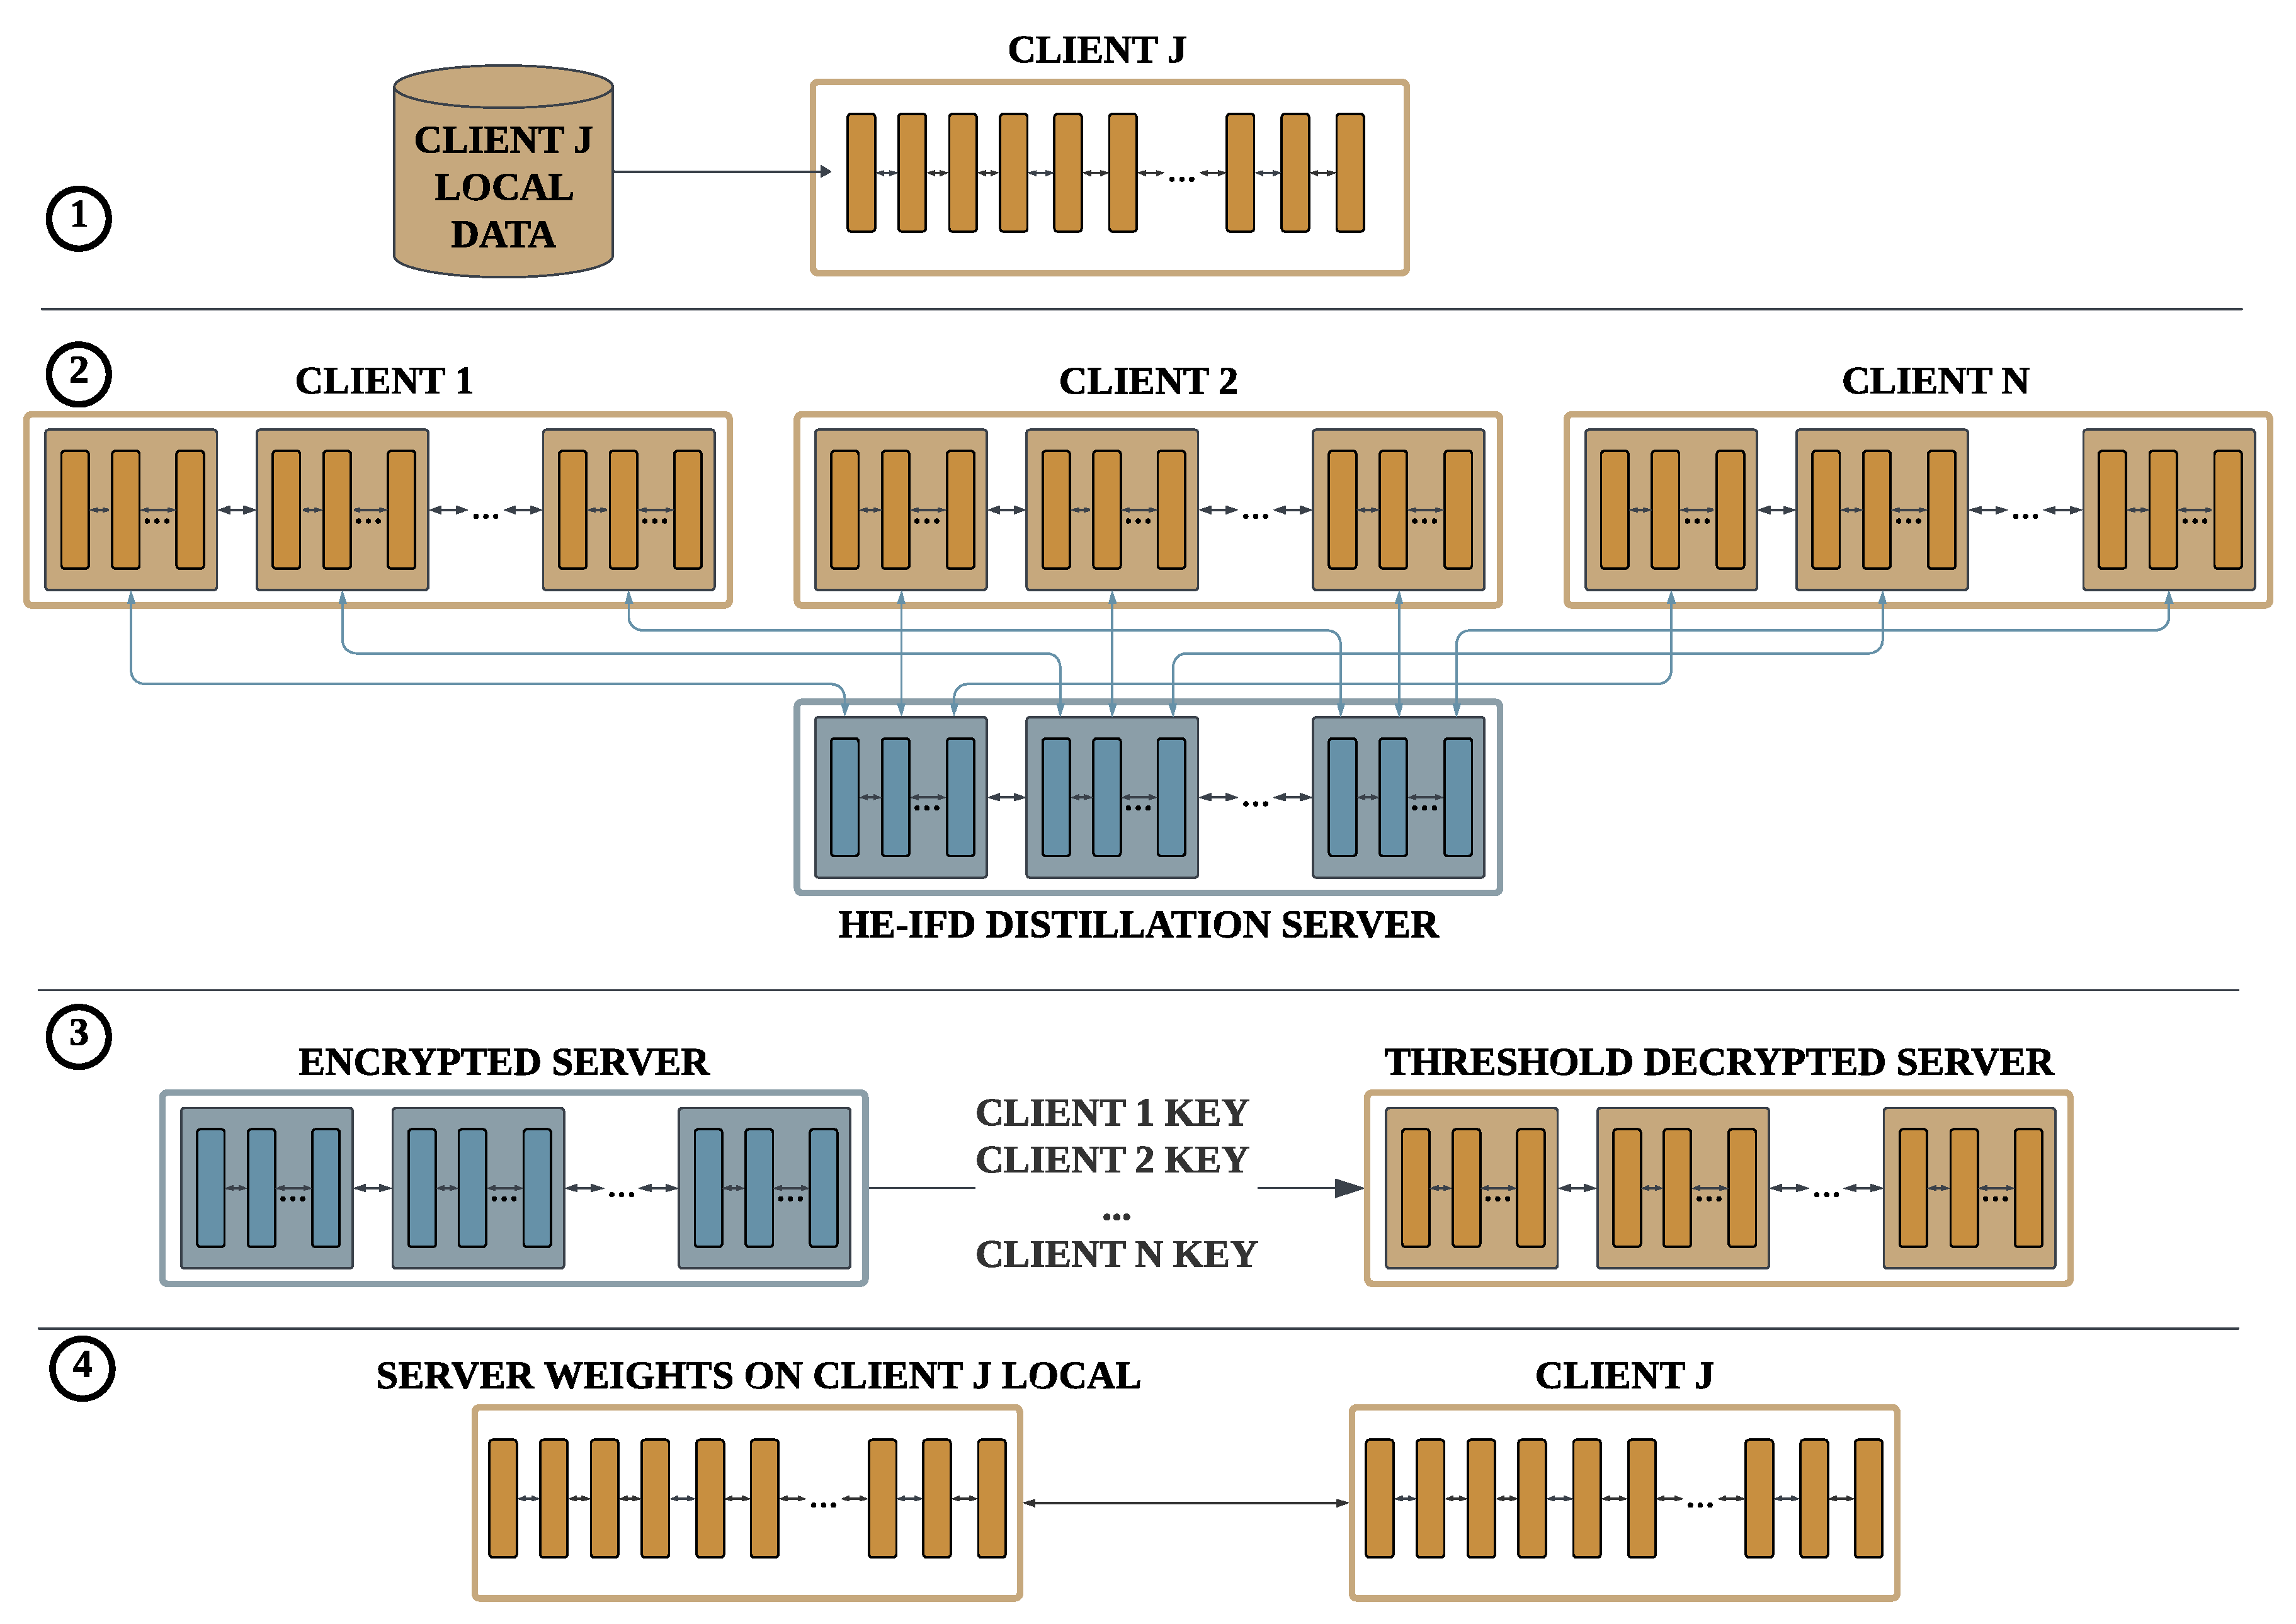
\includegraphics[width=0.87\textwidth]{figures/HE-IFD_sysFigure.pdf}
\caption{Overview of HE-IFD. \textcircled{1}~\textbf{Client-side training.} Each client independently trains a teacher model on its own private dataset. No data leaves the client device. \textcircled{2}~\textbf{Encrypted upload and server distillation.} Every client extracts intermediate feature representations at each block boundary of its teacher, normalises them per channel, encrypts them under the CKKS homomorphic encryption scheme, and uploads the ciphertexts to the server in a single communication round. The server pools encrypted features from all clients and trains a student model block by block, operating entirely on ciphertexts. The server never observes any plaintext data, weights, or intermediate values. \textcircled{3}~\textbf{Threshold decryption.} The server distributes the encrypted student model to all clients. Each client applies its secret key share locally to decrypt the model on its own device. No single client can decrypt alone, and the server never sees plaintext weights. \textcircled{4}~\textbf{Local model assembly.} Each client holds the decrypted student model in plaintext and may optionally fine-tune it on local data to adapt to its own distribution, with no further communication required.}
\label{fig:sys_figure}
\end{figure*}

\subsection{HE-IFD: One-Shot Distillation Framework}
\label{sec:framework}

This section presents the HE-IFD protocol in full generality. The framework applies to any architecture that admits a block decomposition with HE-compatible operations; architecture-specific instantiations are deferred to Section~\ref{sec:architecture}.

% \subsubsection{System Model and Threat Model}
% \label{sec:system_model}

\par\noindent\textbf{System Model.} We consider a cross-silo federated learning setting with $N$ clients and a central server. Each client $i$ holds a private dataset $\mathcal{D}_i$ that is never shared or transmitted. Clients wish to collaboratively train a shared student model by transferring knowledge from their locally trained teacher models to the server, without exposing their private data, including raw training data and any intermediate representations. Communication between clients and the server is restricted to a single round: each client sends a set of encrypted messages derived from its local data and model, after which the server performs all remaining computation independently with no further client interaction. An optional release phase at the end allows clients to collectively obtain the trained model.

\par\noindent\textbf{Threat Model.} We assume a semi-honest (honest-but-curious) server that follows the protocol faithfully but may attempt to infer private information from everything it observes. The adversary's goal is to infer information about a client's private dataset $\mathcal{D}_i$ or the client's local model, including individual samples, label distributions, or model weights, from the messages it receives during training. We further assume that the server may collude with up to $N-1$ clients; privacy of the remaining honest client's input is guaranteed by the threshold structure of the multiparty CKKS scheme described in Section~\ref{sec:phase3}, which requires the joint participation of all $N$ clients to decrypt any ciphertext.

Given this system and threat model, sending plaintext teacher outputs to the server is insufficient. Because, as discussed in Section~\ref{sec:bg_server_inference}, even a single round of plaintext knowledge transfer exposes clients to inference and inversion attacks. We therefore instantiate the knowledge transfer channel using the multiparty CKKS HE scheme~\cite{cheon2017ckks, mouchet2021multiparty} — the same construction implemented in Lattigo~\cite{lattigo} — which lets the server perform all distillation computation directly on ciphertexts under a public key whose corresponding secret key is held in shares across the $N$ clients.

% Under the IND-CPA security of CKKS, the server's entire view during training (encrypted feature pairs, intermediate activations, loss values, gradients, and student weights) is computationally indistinguishable from random. The server operates purely as a blind compute delegate and learns nothing about any client's private data. For additional protection, clients may add calibrated differential privacy noise before encryption, achieving $(\epsilon, \delta)$-differential privacy for the released model; this is optional since the cryptographic guarantee already prevents the server from inspecting any individual contribution during training.


% \subsubsection{Overview of HE-IFD}
% \label{sec:overview}

\par\noindent\textbf{Overview of HE-IFD.} HE-IFD proceeds in four phases, illustrated in Figure~\ref{fig:sys_figure} and formalised in Algorithm~\ref{alg:heifd}. In Phase~1, each client independently trains a teacher model on its private data. In Phase~2, clients extract intermediate features at each block boundary of the teacher, encrypt them under CKKS, and upload to the server in a single communication round, which is the only client-to-server interaction in the entire protocol. The server then trains an HE-compatible student model block by block on the pooled encrypted features. In Phase~3, clients collaboratively perform threshold decryption to obtain the trained student in plaintext. In Phase~4, each client receives the decrypted model (via joint threshold decryption) and may fine-tune it on local data to adapt to its own distribution.

The server never sees any plaintext data, model weights, or intermediate computations. All training happens on encrypted ciphertexts. Each block is trained independently with fresh ciphertexts, so multiplicative levels do not accumulate across blocks.


\begin{algorithm}[t!]
\small
\caption{HE-IFD: HE-Based Intermediate Feature Distillation}
\label{alg:heifd}
\begin{algorithmic}[1]
\REQUIRE $N$ clients with private datasets $\mathcal{D}_1, \ldots, \mathcal{D}_N$; student architecture $S$ with $K{+}1$ blocks
\ENSURE Trained student model $S$

\STATE \textbf{--- Phase 1: Client-Side Training (parallel, local) ---}
\FOR{each client $i = 1, \ldots, N$ \textbf{in parallel}}
    \STATE Train teacher $T_i$ on $\mathcal{D}_i$ via standard SGD
\ENDFOR

\STATE
\STATE \textbf{--- Phase 2: Encrypted Upload + Server Distillation ---}
\FOR{each client $i = 1, \ldots, N$ \textbf{in parallel}}
    \FOR{each block $k = 0, \ldots, K$}
        \STATE Extract feature pairs $(\mathbf{x}_k^{(i,j)}, \mathbf{y}_k^{(i,j)})$ by running $T_i$ on $\mathcal{D}_i$
        \STATE Normalise per channel: $\tilde{\mathbf{y}}_k \leftarrow (\mathbf{y}_k - \mu) / \sigma$ \hfill\COMMENT{Eq.~\ref{eq:client_norm}}
    \ENDFOR
    \STATE Encrypt all pairs under CKKS; upload $\{\enc{\mathbf{x}_k}, \enc{\tilde{\mathbf{y}}_k}\}$ to server \hfill\COMMENT{one-shot}
\ENDFOR

\STATE
\STATE \textit{Server-side (all computation on encrypted data):}
\STATE Initialise student $S$ with near-linear polynomial activations
\FOR{block $k = 0, \ldots, K$}
    \STATE Pool encrypted pairs from all $N$ clients for block $k$; shuffle
    \STATE Set depth-dependent hyperparameters: $\lambda_k, \eta_k$ \hfill\COMMENT{deeper blocks: stronger reg., lower LR}
    \FOR{epoch $= 1, \ldots, E$}
        \FOR{each mini-batch $(\enc{\mathbf{x}}, \enc{\tilde{\mathbf{y}}_k})$}
            \STATE $\hat{\mathbf{y}} \leftarrow S_{\text{block}[k]}(\enc{\mathbf{x}})$ \hfill\COMMENT{encrypted forward pass}
            \STATE $\mathcal{L} \leftarrow \mathcal{L}_{\text{MagReg}}(\hat{\mathbf{y}}, \enc{\tilde{\mathbf{y}}_k})$ \hfill\COMMENT{Eq.~\ref{eq:magreg}}
            \STATE Update $S_{\text{block}[k]}$ via encrypted gradient descent
        \ENDFOR
    \ENDFOR
    \STATE Freeze $S_{\text{block}[k]}$; initialise bridge $\mathbf{b}_k$ from feature statistics
\ENDFOR
\STATE Refine blocks sequentially with bridges on uploaded features ($R$ rounds)

\STATE
\STATE \textbf{--- Phase 3: Threshold Decryption ---}
\STATE All $N$ clients contribute key shares $\rightarrow$ decrypt $S$ to plaintext

\STATE
\STATE \textbf{--- Phase 4: Client-Side Model Assembly ---}
\FOR{each client $i = 1, \ldots, N$}
    \STATE Receive decrypted student $S$
    \STATE (Optional) Fine-tune $S$ on local data $\mathcal{D}_i$ with cross-entropy loss
\ENDFOR
\end{algorithmic}
\end{algorithm}

\subsubsection{Phase~1: Client-Side Training}
\label{sec:phase1}

Each client $i$ trains a teacher model $T_i$ on its private data $\mathcal{D}_i$ using standard supervised learning. All clients start from the same shared random weight initialisation. This phase is fully local, and no data leaves the client device.


\subsubsection{Phase~2: Encrypted Upload and Server-Side Distillation}
\label{sec:phase2}

Phase~2 has two parts: first, clients extract and upload encrypted features (one-shot); then, the server trains a student model entirely on these encrypted features.

\par\noindent\textbf{Feature extraction.} Each client runs its trained teacher on local data and extracts input-output feature pairs $(\mathbf{x}_k, \mathbf{y}_k)$ at every block boundary $k \in \{0, \ldots, K\}$, where block boundaries match the student architecture (Section~\ref{sec:architecture}). Clients use their own local data, not a shared auxiliary dataset. This is important: each teacher produces high-confidence outputs for the classes it has seen, and using local data preserves this specialisation rather than diluting it with uncertain predictions on unfamiliar classes.

\par\noindent\textbf{Normalisation.} Consistent normalisation across clients is essential for stable encrypted training. We adopt a collaborative normalisation approach where each client computes local statistics and the server aggregates them on encrypted data, following the privacy-preserving federated normalisation framework of~\cite{cosgun2025federated}. Before encryption, each client normalises features per channel to zero mean and unit variance:
\begin{equation}
    \mu_c^{(k,i)} = \mathbb{E}_{x \in \mathcal{D}_i}\!\left[ y_{k,c}(x) \right], \quad
    \sigma_c^{(k,i)} = \text{Std}_{x \in \mathcal{D}_i}\!\left[ y_{k,c}(x) \right]
    \label{eq:client_stats}
\end{equation}
\begin{equation}
    \tilde{y}_{k,c} = \frac{y_{k,c} - \mu_c^{(k,i)}}{\sigma_c^{(k,i)}}
    \label{eq:client_norm}
\end{equation}
where $y_{k,c}$ is the output of channel $c$ at block boundary $k$, $\mathbb{E}[\cdot]$ and $\text{Std}[\cdot]$ denote the mean and standard deviation over all samples in client $i$'s local dataset $\mathcal{D}_i$, and $C$ is the total number of channels at that block boundary. This is not optional since, without it, teachers trained on different distributions produce features with incompatible magnitude ranges, and the server's training diverges when pooling them.

\par\noindent\textbf{Encrypted upload.} Clients encrypt normalised features under CKKS and upload to the server. This is a single communication round and no further client interaction is needed. Normalisation statistics ($2C$ values per block per client, where $C$ is the number of channels)) may be sent in plaintext since they are aggregate quantities that reveal unimportant information about individual samples.


\par\noindent\textbf{Server-side distillation.} The server trains the student model block by block on the pooled encrypted features from all clients. For each block $k$, the server receives fresh encrypted input-output pairs $\left(\enc{\mathbf{x}_k^{(i,j)}},\, \enc{\tilde{\mathbf{y}}_k^{(i,j)}}\right)$ from every client $i$. It pools and shuffles them, then trains block $k$ via encrypted gradient descent. Upon convergence, block $k$ is frozen and the server moves to block $k{+}1$ using fresh ciphertexts.

This is the key design choice: each block trains on its own fresh ciphertexts, so CKKS multiplicative levels never accumulate across blocks. The total depth per block depends only on that block's structure, regardless of network depth.

Unlike federated averaging, the server does not aggregate teacher outputs. Each client's features provide independent gradient steps that accumulate into shared student weights. A client who specialises in certain classes contributes strong supervision for those classes, with no signal dilution.

\par\noindent\textbf{Train-inference distribution gap.} When block $k$ is trained on teacher features (ReLU-based: non-negative, sparse) but receives student features at inference (polynomial: signed, dense), a distribution gap arises. Empirically, composed accuracy collapses to ${\sim}10\%$ without addressing this.

We close this gap within the one-shot protocol by having each block trained in two stages. In the first stage, the block is trained on teacher features to learn the correct mapping. In the second stage (refinement), the block is fine-tuned on the uploaded encrypted data with a per-channel affine \textit{TrainableBridge} $\mathbf{b}_k(\mathbf{h}) = \boldsymbol{\gamma}_k \odot \mathbf{h} + \boldsymbol{\beta}_k$ that compensates for the distribution shift. Bridge parameters are initialised from feature statistics and co-trained with block weights during refinement.


\par\noindent\textbf{Loss Function.} Each block is trained with a magnitude-regularised normalised mean squared error loss. Student and teacher features are normalised per channel to zero mean and unit variance before computing the error:
\begin{equation}
    \mathcal{L}_{\text{NormMSE}} = \frac{1}{C} \sum_{c=1}^{C} \text{MSE}\!\left(\frac{\hat{f}_c - \mu_{\hat{f}_c}}{\sigma_{\hat{f}_c}},\; \frac{\tilde{f}_c - \mu_{\tilde{f}_c}}{\sigma_{\tilde{f}_c}}\right)
    \label{eq:normmse}
\end{equation}
where $\hat{f}_c$ and $\tilde{f}_c$ are the student prediction and normalised teacher target for channel $c$. This scale-invariant loss handles the distributional mismatch between student activations (signed, potentially large) and teacher activations.

\par\noindent\textbf{Magnitude regularisation.} The normalised loss alone is scale-invariant and permits the student to grow magnitudes without penalty. Since subsequent frozen polynomial blocks amplify any scale drift, we add a log-ratio penalty:
\begin{equation}
    \mathcal{L}_{\text{MagReg}} = \mathcal{L}_{\text{NormMSE}} + \lambda \cdot \frac{1}{C} \sum_{c=1}^{C} \left(\log \frac{\sigma_{\hat{f}_c}}{\sigma_{\tilde{f}_c}}\right)^{\!2}
    \label{eq:magreg}
\end{equation}
The log-ratio form is symmetric (penalising student magnitudes that are too large or too small equally) and scale-free (proportional to the multiplicative mismatch). The regularisation weight $\lambda$ scales with block depth: stronger regularisation is applied to deeper blocks where magnitude accumulation from the frozen chain is more severe.

\par\noindent\textbf{MSE on logits.} For the head block (block $K$), which outputs class logits, we use plain MSE without normalisation or magnitude regularisation, since logits are low-dimensional and do not exhibit the spatial channel structure of intermediate features. We use MSE rather than KL divergence because softmax is not a polynomial operation and cannot be evaluated under CKKS encryption. MSE on raw logits is HE-compatible because the squaring operation requires one ciphertext-ciphertext multiplication, and the remaining subtraction and averaging are level-free.


\subsubsection{Phase~3: Threshold Decryption}
\label{sec:phase3}

We instantiate the encrypted channel of HE-IFD with the multiparty CKKS protocol of~\cite{mouchet2021multiparty}, available in the open-source Lattigo library~\cite{lattigo}. We describe how the protocol is used in HE-IFD; the underlying construction is unchanged from the cited references and we treat it as a black box.

\par\noindent\textbf{Setup (before Phase~1).} The $N$ clients run a distributed key generation (DKG) protocol with no trusted dealer. Each client $i$ samples a secret-key share $\mathsf{sk}_i$ from the CKKS secret-key distribution and contributes a corresponding share to the protocol. The DKG output is (i)~a collective public key $\mathsf{pk}$ usable by everyone for encryption, (ii)~collective evaluation and rotation keys usable by the server for homomorphic computation, and (iii)~the secret-key shares $\{\mathsf{sk}_i\}_{i=1}^{N}$, kept privately by the clients. The full secret key $\mathsf{sk} = \sum_{i=1}^{N} \mathsf{sk}_i$ is never assembled at any single party at any point in the protocol.

\par\noindent\textbf{Encryption (Phase~2).} Every client encrypts its normalised feature pairs (Section~\ref{sec:phase2}) under the collective public key $\mathsf{pk}$ and uploads the ciphertexts to the server. From the server's perspective, the resulting ciphertexts behave exactly as ordinary single-key CKKS ciphertexts: the server applies homomorphic additions, ciphertext-by-plaintext multiplications, ciphertext-by-ciphertext multiplications (using the collective relinearisation key), and slot rotations (using the collective rotation keys) in the usual way. No client interaction is required during this phase.

\par\noindent\textbf{Collective decryption (Phase~3).} To release the trained student in plaintext, the server initiates a single round of \emph{collective key-switching}~\cite{mouchet2021multiparty}: it broadcasts the encrypted student weights $\enc{\mathbf{W}}$ to the clients, and each client $i$ contributes a key-switching share that re-encrypts $\enc{\mathbf{W}}$ from the collective key $\mathsf{pk}$ to a target key $\mathsf{pk}'$ (e.g., the all-zero key, which yields plaintext, or a fresh public key whose corresponding secret is held by a designated recipient). Every client's share is computed locally from $\mathsf{sk}_i$ and added a small smudging noise to mask its individual contribution. Combining all $N$ shares yields the re-encrypted ciphertext, from which $\mathbf{W}$ can be decrypted; combining any strict subset of $N-1$ shares yields a uniformly random ring element under the RLWE assumption~\cite{lyubashevsky2010ideal}. If this phase is skipped, the student stays encrypted and the server can serve encrypted inference directly.

\par\noindent\textbf{Trust assumption.} Privacy of every client's input holds as long as at least one of the $N$ clients is honest. This is strictly stronger than the trust assumption of single-key CKKS deployments, which require a trusted decryption authority, and matches the threat model of Section~\ref{sec:framework}: even if the server colludes with $N-1$ clients, the joint view consists of ciphertexts under a key whose remaining share is held by the honest client and is therefore computationally indistinguishable from random.


\subsubsection{Phase~4: Client-Side Model Assembly and Fine-Tuning}
\label{sec:phase4}

After local decryption, each client holds a copy of the trained student model in plaintext. Clients may fine-tune this model on their own private data using standard cross-entropy loss. This step requires no further communication with the server or other clients. Fine-tuning is particularly useful under non-IID settings, where the global student may underperform on a client's local distribution. We evaluate the accuracy impact of local fine-tuning in Section~\ref{sec:experiments}.


% \subsubsection{Algorithm}
% \label{sec:algorithm}


\subsection{Training Stability}
\label{sec:stability}

As established in Section~\ref{sec:introduction}, the composition of degree-$d$ polynomial activations across $L$ blocks yields an end-to-end map of degree $d^L$, whose magnitude bound grows doubly-exponentially in depth. This is a property of the function class rather than of any particular implementation, and it must be controlled by a combination of mechanisms that act on different parts of the protocol. Concretely:

\begin{itemize}[leftmargin=*,nosep]
    \item \textbf{Client-side normalisation} (Eq.~\ref{eq:client_norm}): ensures features from different clients have compatible magnitude ranges.
    \item \textbf{Magnitude-regularised loss} (Eq.~\ref{eq:magreg}): penalises scale drift between student and teacher outputs.
    \item \textbf{Gradient clipping}: prevents large updates from the quadratic term.
    \item \textbf{Depth-dependent hyperparameters}: deeper blocks use stronger regularisation and lower learning rates.
    \item \textbf{Per-channel affine bridges}: compensate for the absence of batch normalisation at block boundaries.
\end{itemize}

Section~\ref{sec:experiments} provides an ablation study quantifying the impact of each mechanism.


%% ================================================================
\subsection{Privacy Analysis}
\label{sec:privacy_proof}

%We provide a formal privacy argument for the HE-IFD protocol. 
%We assume the server is honest-but-curious: it follows the protocol but may try to learn client data from what it sees. We assume all $N$ clients are honest. 
During Phase~2, the server sees only CKKS-encrypted data: teacher block-boundary feature pairs, basic metadata such as tensor shapes and client count, and optional plaintext per-channel normalisation statistics. Raw client data and teacher model weights never leave the client. All server-side computations, i.e., forward passes, loss evaluation, gradient descent, and weight updates, are performed homomorphically on ciphertexts; student weights, intermediate activations, gradients, and loss values remain encrypted throughout Phase~2.

Under the Ring Learning with Errors (RLWE) assumption (with security parameter $\lambda \geq 128$), our protocol guarantees that the server learns no private information about individual client data during training. This relies on the IND-CPA security of the CKKS scheme~\cite{cheon2017ckks}, which means encrypted data cannot be distinguished from random noise. Because all homomorphic operations simply map ciphertexts to other ciphertexts, every intermediate calculation stays secure. As a result, the server's entire view of the training process can be simulated using only public parameters and metadata, proving no data is leaked. If clients choose to send their normalisation statistics in plaintext, these are aggregate quantities computed over the full local dataset and carry negligible information about any individual sample. For maximum security, these statistics can also be encrypted following the protocols in~\cite{cosgun2025federated}.

% If clients choose to decrypt the trained model for release, the resulting plaintext model has the same risk of membership inference attacks~\cite{shokri2017membership, carlini2022membership} as any standard machine learning model. Homomorphic encryption prevents data leakage during training without adding noise or limiting the number of training steps. In contrast, differential privacy adds noise to protect the final model, which lowers accuracy and limits how much training can be done. However, our protocol easily supports both: clients can add differential privacy noise to their data before encrypting it. This provides a formal $(\epsilon, \delta)$-differential privacy guarantee for the final decrypted model without changing how the encrypted training works.


%% ================================================================
\subsection{Architecture-Specific Instantiations}
\label{sec:architecture}

The HE-IFD framework described in Section~\ref{sec:framework} applies to any neural network that can be decomposed into blocks with HE-compatible operations. This section describes how we instantiate the framework for convolutional networks and vision transformers. The same principles extend to language models, which we discuss briefly for completeness.


\subsubsection{Convolutional Networks}
\label{sec:arch_cnn}

\par\noindent\textbf{PolyResNet-18.} The primary convolutional instantiation is PolyResNet-18, which is structurally identical to the ResNet-18 teacher but with all HE-incompatible operations replaced. This structural correspondence enables block-level feature matching between teacher and student. We summarize the replacements below: 

\par\noindent\textbf{ReLU $\to$ PolyAct.} ReLU ($\max(0, x)$) has no efficient polynomial representation under CKKS. We replace it with a learnable degree-2 polynomial:
\begin{equation}
    \text{PolyAct}(x) = ax^2 + bx + c
    \label{eq:polyact}
\end{equation}
initialised at $a = 0.3$, $b = 0.7$, $c = 0$, so that for normalised inputs the activation behaves approximately linearly, avoiding early magnitude divergence from the quadratic term. This near-linear initialisation strategy is consistent with prior work on stable polynomial-activation training~\cite{baruch2022methodology, garimella2021sisyphus}. The coefficients are learnable and adapt during training; after training, they are frozen as plaintext constants. Under CKKS, $x^2$ is one ciphertext-ciphertext multiplication (1 multiplicative level). The remaining terms ($ax^2, bx, c$) involve only plaintext-ciphertext operations (0 levels). Thus, the total cost is 1 multiplicative level per activation.

\par\noindent\textbf{BatchNorm $\to$ ChannelScale.} Batch normalisation computes a normalised output $\hat{x} = (x - \mu)/\sigma$ followed by a learnable affine transform. Under CKKS, the division $x/\sigma$ has no direct equivalent and must be approximated via iterative methods such as Goldschmidt's algorithm, which requires approximately 10 multiplicative levels per invocation. Since batch statistics are fixed after training, the normalisation can be folded into the affine parameters, leaving only the learnable scale and bias. We therefore replace BatchNorm with ChannelScale:
\begin{equation}
    \text{ChannelScale}(x) = \gamma \odot x + \beta
    \label{eq:channelscale}
\end{equation}
with learnable $\gamma$ (initialised to 1) and $\beta$ (initialised to 0). Since both are known plaintext at inference, this costs 0 multiplicative levels.

\par\noindent\textbf{MaxPool $\to$ Identity.} Max pooling is a comparison operation that requires non-polynomial approximations with prohibitive multiplicative depth under CKKS. For CIFAR-10 (32$\times$32 input), the initial max pool in standard ResNet-18 is replaced by an identity operation. Spatial downsampling is handled by stride-2 convolutions in deeper layers.

\par\noindent\textbf{PolyBasicBlock.} Each PolyBasicBlock, the residual building block of PolyResNet-18, follows the dataflow:
\begin{equation}
    x \xrightarrow{\text{conv}_1} \xrightarrow{\text{CS}_1} \xrightarrow{\text{PolyAct}_1} \xrightarrow{\text{conv}_2} \xrightarrow{\text{CS}_2} \xrightarrow{+\,\text{identity}} \xrightarrow{\text{PolyAct}_2} y
\end{equation}
where CS denotes ChannelScale and $+\,\text{identity}$ is the residual addition. Convolutions, ChannelScale, and the residual addition do not consume any levels. The two PolyAct invocations consume 1 level each, for a total of 2 multiplicative levels per block.

\par\noindent\textbf{Block boundaries.} We define six blocks for ResNet-18: Block~0 (stem) takes raw images as input and outputs the result after the first convolution, ChannelScale, and PolyAct. Blocks~1 through~4 correspond to the four residual layer groups, each containing two PolyBasicBlocks. Block~5 (head) processes the final layer's output into class logits via average pooling and a fully connected layer.

\par\noindent\textbf{Compact variants and simpler architectures.} We also evaluate PolyResNet-10 (one block per layer instead of two, approximately 5.6 million parameters) and PolyResNet-8 (three layers instead of four, approximately 1.5 million parameters) to study the effect of model capacity. For lightweight settings, we instantiate HEStudentCNN, a plain convolutional network with configurable channel widths, polynomial activations, and per-channel affine normalisation (no residual connections). These compact architectures demonstrate that the framework generalises beyond the ResNet family.


\subsubsection{Transformer and Vision Transformer Architectures}
\label{sec:arch_transformer}

HE-IFD naturally extends to transformer-based models through logit-level KL distillation rather than block-level feature matching. Transformer attention mechanisms create inter-layer dependencies that make intermediate feature matching less effective, but logit-level distillation requires only that the student match the teacher's final output distribution.

A key advantage of HE-IFD for transformers is its compatibility with pre-trained models. Rather than training from scratch, each client fine-tunes a pre-trained model (e.g., ViT-B/32 pre-trained on ImageNet) on their local data in Phase 1. This makes the framework practical for large models that would be infeasible to train from scratch on small client datasets. After encrypted distillation (Phase 2) and threshold decryption (Phase 3), clients receive the student model and may further fine-tune it locally in Phase 4 using standard (non-polynomial) activations, recovering any accuracy lost from HE-compatible replacements.

\par\noindent\textbf{Vision Transformer (ViT).} In Phase 1, each client takes a ViT-B/32 model pre-trained on ImageNet-1K (88M parameters) and fine-tunes it on their local private data partition to produce a teacher. In Phase 2, clients extract logits from their fine-tuned teachers, encrypt them, and upload to the server. The server distils these into an HE-compatible student where GELU activations are replaced with PolyGELU (degree-4 polynomial) and LayerNorm with AffineNorm. We evaluate on CIFAR-10 and FashionMNIST.


% \par\noindent\textbf{Language models (future work).} The same logit-level distillation extends to language models such as GPT-2 and DistilBERT by fine-tuning pre-trained models on client data partitions. Our preliminary experiments show that stable polynomial training for deep language models remains challenging, and we leave a full evaluation to future work.

\par\noindent\textbf{HE-compatible replacements for transformers.} Two operations in standard transformers are incompatible with CKKS: the GELU activation function and LayerNorm. We replace GELU with a degree-4 polynomial approximation (PolyGELU) fitted to match GELU over the range $[-5, 5]$. LayerNorm, which requires a division by the standard deviation, is replaced by AffineNorm: a per-element learnable scale and bias without any running statistics or normalisation division. These replacements are analogous to the PolyAct and ChannelScale substitutions in the convolutional setting.

\par\noindent\textbf{HE compliant student training.} To ease optimisation, we train transformer students in two phases. In the warmup phase, the student retains the standard GELU and LayerNorm activations, and is trained with KL divergence loss for several epochs to converge to a good parameter region. In the conversion phase, all GELU activations are replaced with PolyGELU and all LayerNorm layers are replaced with AffineNorm, and training continues with a reduced learning rate to adapt to the polynomial activation landscape. This two-phase strategy avoids the difficulty of training with polynomial activations from scratch, which we found to be unstable for transformer architectures.

\par\noindent\textbf{Memory efficiency.} For models with large output spaces, teacher logit tensors can be very large. We store averaged logits in half precision (float16), which halves memory usage with negligible impact on distillation quality. Logit averaging across clients is performed via in-place accumulation rather than stacking, reducing peak memory from three times the logit tensor size to two times.


%% ================================================================
\subsection{Communication and Computation Complexity}
\label{sec:complexity}

\subsubsection{CKKS Multiplication Budget}
\label{sec:ckks_budget}

Each ciphertext-ciphertext (CT$\times$CT) multiplication consumes one multiplicative level. Ciphertext-plaintext (CT$\times$PT) multiplications and all additions are level-free. Once a ciphertext's levels are exhausted, bootstrapping can refresh them, but at high computational cost.

On the server, \textbf{both the student weights and the client features are encrypted ciphertexts}. The server never holds plaintext weights or data. Every learnable operation (convolution, affine scaling, fully connected layers) is CT$\times$CT and consumes 1 level. Polynomial activations of degree $d$ consume $\lceil \log_2 d \rceil$ levels (e.g., degree-2 costs 1 level for $x^2$, degree-4 costs 2 levels for $x^2 \to x^4$). Additions (residual connections, bias terms) and plaintext-scalar operations (average pooling) are level-free, consuming no multiplicative depth.

\par\noindent\textbf{Per-block training depth.} HE-IFD trains each block independently with fresh ciphertexts, so levels never accumulate across blocks during Phase 2a. The depth consumed per block depends only on that block's internal structure. For the architectures we evaluate, a single block's forward pass consumes 4--16 levels depending on complexity. Adding loss computation (1 level for MSE) and the backward pass, the total per-block training depth fits within the budget provided by ring dimension $\log \mathcal{N} = 15$ (${\sim}$18 levels at 128-bit security). Phase 2a therefore, requires no bootstrapping. The cascade refinement in Phase 2b composes multiple blocks and exceeds the per-block budget, requiring bootstrapping to refresh levels between blocks (Section~\ref{sec:comm_comp}).


\par\noindent\textbf{Post-decryption inference.} After threshold decryption (Phase~3), weights become plaintext. Since weights are now plaintext constants, learnable operations (convolution, affine scaling) become plaintext-by-ciphertext multiplications, which do not consume multiplicative levels. Only polynomial activations, which involve ciphertext-by-ciphertext squaring, still consume levels.


\subsubsection{Computational Cost}
\label{sec:comp_cost}

On the client side, the dominating cost is training the local teacher model, which is standard supervised learning and scales with the size of each client's dataset. Feature extraction requires a single forward pass through the trained teacher and is comparatively inexpensive.

On the server side, training proceeds block by block. For each block, the server performs encrypted gradient descent over pooled client data. The per-iteration cost is higher than plaintext training due to CKKS ciphertext operations, but the total number of iterations is modest because the block-level supervision signal is direct (input-output pairs rather than end-to-end labels). 
% Refinement operates on features already held by the server and incurs no additional communication cost.

\subsubsection{Communication Cost}
\label{sec:comm_cost}

HE-IFD requires only a single communication round from each client to the server. The upload consists of encrypted input-output feature pairs for each block, plus per-channel normalisation statistics.

The dominant cost comes from encrypting intermediate feature maps, whose dimensionality far exceeds the normalisation statistics ($2C$ scalars) and evaluation keys (uploaded once per client). The total per-client upload volume is:
\begin{equation}
    C_{\text{client}} = \sum_{k=0}^{K} \left\lceil \frac{D_k}{S} \right\rceil \times N_{\text{samples}} \times C_{\text{CT}}
    \label{eq:comm_cost}
\end{equation}
where $D_k$ is the feature dimensionality at block boundary $k$, $S$ is the number of CKKS slots per ciphertext, $N_{\text{samples}}$ is the number of samples each client uploads, and $C_{\text{CT}}$ is the size of one ciphertext.

As a concrete example, in the ResNet-18 instantiation, Block~1 (the first residual layer group) produces feature maps of shape $64 \times 32 \times 32 = 65{,}536$ elements per sample. With 4096 CKKS slots per ciphertext (at ring dimension $\log \mathcal{N} = 13$), a single sample requires 16 ciphertexts per block boundary. Using 10\% of a 5000-sample local dataset gives 500 samples per client, amounting to 8{,}000 ciphertexts for Block~1 alone. At approximately 0.6~MB per ciphertext, this gives roughly 4.8~GB per client per block.

For transformer architectures using logit-level distillation, the communication cost depends on the output dimensionality and the number of samples. For ViT-B/32 on CIFAR-10 (10 classes), each client uploads encrypted logits for 5000 samples, which is modest (${\sim}$0.2~MB). For language models with large vocabularies, the cost is higher: a model with 50,000 output tokens and 5000 sequences of length 128 would produce a logit tensor of ${\sim}$48~GB in float32 or ${\sim}$24~GB in float16. Since logit-level distillation uses only a single "block" (the full model output), this is the total per-client upload. Note that the communication cost for multi-round encrypted FL \cite{sav2021poseidon,zhang2020batchcrypt} would be orders of magnitude larger, as each of the hundreds of training rounds requires encrypting and uploading full model gradient updates from every client. Vanilla (unencrypted) FL avoids encryption overhead but provides no privacy protection. In both cases, the HE-IFD upload is performed once and requires no further interaction.

% \section{METHODOLOGY}
% \label{sec:methodology}

% \begin{figure*}[t]
% \centering
% 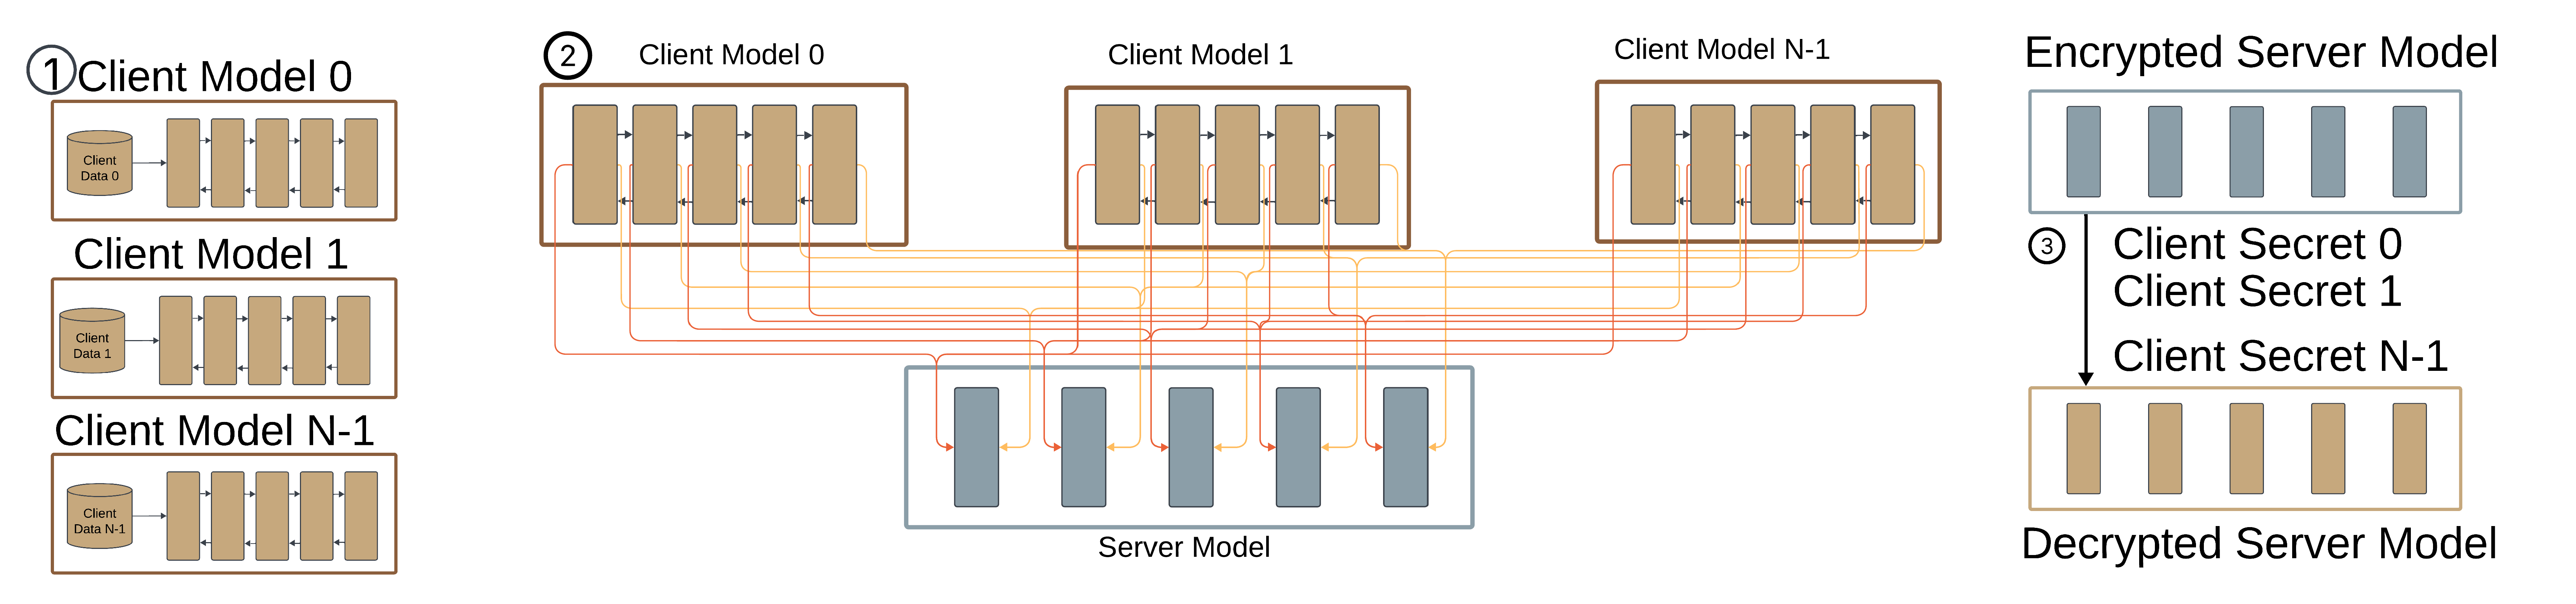
\includegraphics[width=\textwidth]{figures/SysFigureSimple.pdf}

% \caption{Overview of the HE-IFD framework. In Step~1 (Phase~1: Client-Side), each client independently trains a local teacher model on its private dataset, extracts per-block input--output feature pairs, normalises them collaboratively, and encrypts them under CKKS. In Step~2 (Phase~2: Server-Side Distillation), the server acts as a completely blind compute delegate, distilling these encrypted supervision signals block-by-block into an HE-compatible student model (e.g., PolyResNet-18) without ever observing plaintext data, weights, or activations. In Step~3 (Phase~3: Optional Model Release), clients collaboratively perform threshold decryption to release the trained model in plaintext.}

% \label{fig:sys_figure}
% \end{figure*}
 

% \subsection{System Model and Threat Model}
% \label{sec:system_model}

% \par\noindent\textbf{System Model.} We consider a cross-silo federated learning setting with $N$ clients and a central server. Each client $i$ holds a private dataset $\mathcal{D}_i$ that is never shared or transmitted. Clients wish to collaboratively train a shared student model by transferring knowledge from their locally trained teacher models to the server, without exposing their private data, including raw training data and any intermediate logits. Communication between clients and the server is restricted to a single round: each client sends a set of messages derived from its local data and model, after which the server performs all remaining computation independently with no further client interaction. An optional release phase at the end allows clients to collectively obtain the trained model.



% \par\noindent\textbf{Threat Model.} We assume a semi-honest (honest-but-curious) server that follows the protocol faithfully but may attempt to infer private information from everything it observes. All clients are assumed to behave honestly. The adversary's goal is to learn anything about a client's private dataset $\mathcal{D}_i$ or client's local model---including individual samples, label distributions, or model weights---from the messages it receives during training.


% Given this system and threat model, sending plaintext teacher outputs to the server is insufficient: as discussed in Section~\ref{sec:bg_server_inference}, even a single round of plaintext knowledge transfer exposes clients to inference and inversion attacks. We therefore instantiate the knowledge transfer channel using the CKKS homomorphic encryption scheme~\cite{cheon2017ckks}, which allows the server to perform all distillation computation directly on ciphertexts.


% Under the IND-CPA security of CKKS, the server's entire view during training, i.e., encrypted feature pairs, intermediate activations, loss values, gradients, and student weights, is computationally indistinguishable from random. The server operates purely as a blind compute delegate and learns nothing about any client's private data. For additional protection, clients may add calibrated differential privacy noise before encryption, achieving $(\epsilon, \delta)$-differential privacy for the released model; this is optional since the cryptographic guarantee already prevents the server from inspecting any individual contribution during training.



% % \subsubsection{CKKS Depth Budget and Protocol Phases}
% % \label{sec:encryption_params}

% % The CKKS scheme supports approximate arithmetic over real numbers but imposes a finite multiplicative depth budget: each ciphertext--ciphertext multiplication consumes one level, and once exhausted, the ciphertext can no longer be used. HE-IFD manages this budget by design.

% % \textbf{During training}, each block is trained independently with fresh ciphertexts. Since fresh ciphertexts start at full depth, there is no level accumulation across blocks regardless of network depth. The multiplicative depth consumed per block depends only on that block's internal structure: a single PolyBasicBlock containing two degree-2 polynomial activations consumes 2 levels in the forward pass, with additional levels for the backward pass chain rule through the polynomial terms.

% % \textbf{During encrypted inference} (post-deployment), the full student model requires 17 multiplicative levels for a complete forward pass (Section~\ref{sec:ckks_budget}), as the entire network is evaluated as a single encrypted circuit.

% % \textbf{At model release}, if clients elect threshold decryption, the student model weights are decrypted collaboratively and the model can subsequently be used for plaintext inference.


% % \textbf{At model release}, if clients elect threshold decryption, the student model weights are decrypted collaboratively and the model can subsequently be used for plaintext inference.

% \subsection{Overview of HE-IFD}
% \label{sec:overview}

% % Figure~\ref{fig:sys_figure} illustrates the three-phase HE-IFD protocol. In Step~1, each client independently trains a local teacher model on its private data and extracts intermediate feature pairs at each block boundary. In Step~2, clients normalise these features, encrypt them under CKKS, and upload the ciphertexts to the server in a single communication round, which is the only client--server interaction in the entire protocol. In Step~3, the server trains the HE-compatible student model block by block, operating entirely on ciphertexts without ever observing any plaintext data, weights, or activations. At model release, clients may collaboratively perform threshold decryption to obtain the trained student in plaintext; if omitted, the student remains encrypted and can be used directly for encrypted inference.

% HE-IFD proceeds in three phases, illustrated in Figure~\ref{fig:sys_figure} and formalised in Algorithm~\ref{alg:heifd}. In Phase~1, each client independently trains a local teacher model on its private data, extracts intermediate feature pairs at each block boundary, normalises them collaboratively, and uploads the encrypted ciphertexts to the server in a single communication round, which is the only client-to-server interaction in the entire protocol. In Phase~2, the server trains the HE-compatible student model block by block, operating entirely on ciphertexts. This phase proceeds in two stages: Phase~2a, in which each block is trained independently on encrypted teacher features; and Phase~2b, in which the server performs plaintext refinement using trainable bridges to close the train--inference distribution gap, requiring no additional client communication. In the optional Phase~3, clients collaboratively perform threshold decryption to obtain the trained student model in plaintext; if omitted, the student remains encrypted for direct encrypted inference.


% The phases are described in detail below.

% \subsubsection{Phase 1: Client-Side Local Training}
% \label{sec:phase1}

% Each client $i$ trains a local teacher model $T_i$ (e.g., ResNet-18) on their private data $\mathcal{D}_i$ using standard supervised learning. This phase is fully local, ensuring that no data or parameter leaves the client device.

% The server initialises common random weights $\theta_0$ to all clients before local training begins. Each client fine-tunes from $\theta_0$ on their private data. This is standard practice in federated learning and does not constitute a privacy violation: $\theta_0$ is randomly generated and carries no information about any client's data. 
% % In the next section we detail each step in client-side local training.

% % \textbf{Data partitioning.} Data is partitioned across clients using a Dirichlet distribution with concentration parameter $\alpha$, where $\alpha \to 0$ produces extreme non-IID partitions (each client sees few classes) and $\alpha \to \infty$ produces IID partitions. Our experiments evaluate $\alpha \in \{0.1, 0.5, 1.0, 100.0\}$ across $N \in \{1, 2, 4, 8, 16\}$ clients.

% \subsubsection{Phase 2: Per-Block Feature Extraction and Encrypted Upload}
% \label{sec:phase2}

% At a high level, after local training, each client extracts teacher representations at every block boundary, computes normalisation statistics, and uploads encrypted input-output pairs to the server.

% \par\noindent\textbf{Block Boundary Definitions.} We define six blocks matching the teacher and student architectures. Block 0 (stem) takes raw images as input and outputs the result post-conv1, batch normalisation, and ReLU. Block 1 (layer1) takes the stem output and yields features after two BasicBlocks. Blocks 2 through 4 correspond to layers 2 through 4, respectively, incorporating spatial downsampling. Finally, Block 5 (head) processes layer 4 outputs into class logits via average pooling and a fully-connected layer. For each defined block $k$, client $i$ extracts the tuple $(\textbf{x}_k, \textbf{y}_k)$, corresponding respectively to the block's input and output when running the teacher model on local data $\mathcal{D}_i$.

% \par\noindent\textbf{Local Data Protocol.} Each client generates teacher outputs on their \textit{own local training data}~$\mathcal{D}_i$, not on a shared auxiliary dataset. This design has two advantages. First, each teacher evaluates samples from its own training distribution, producing high-confidence supervision signals for the classes it has learned well. A client that specialises in a particular subset of classes provides strong logits and features for those classes, rather than uncertain outputs for classes it has not seen.
% Second, by using each client's data independently without aggregation, the signal from every individual client is preserved at full strength. Under the auxiliary-data protocol (evaluated as a comparison baseline in Section~\ref{sec:experiments}), averaging dilutes the useful signal from specialist clients with weak contributions from clients that have not seen the relevant classes.

% \par\noindent\textbf{Client-Side Collaborative Normalisation.} Before encryption, each client computes per-channel mean and standard deviation over their block-$k$ outputs. 
% For each channel $c$, they normalise their targets to zero mean and unit variance per channel before encryption:
% \begin{equation}
%     \mu_c^{(k,i)} = \mathbb{E}_{x \in \mathcal{D}_i}\!\left[ y_{k,c}(x) \right], \quad
%     \sigma_c^{(k,i)} = \text{Std}_{x \in \mathcal{D}_i}\!\left[ y_{k,c}(x) \right]
%     \label{eq:client_stats}
% \end{equation}
% \begin{equation}
%     \tilde{y}_{k,c} = \frac{y_{k,c} - \mu_c^{(k,i)}}{\sigma_c^{(k,i)}}
%     \label{eq:client_norm}
% \end{equation}
% where $\mu_c^{(k,i)}$ is the per-channel mean, $\sigma_c^{(k,i)}$ is the per-channel standard deviation, $y_{k,c}(x)$ is the $c$-th channel output of block $k$ for input $x$, and $\mathbb{E}$ and $\text{Std}$ denote expectation and standard deviation over the client's local dataset $\mathcal{D}_i$.



% This normalisation is a core component of the protocol, not an optional enhancement. Without it, teachers trained on different data distributions produce features with incompatible magnitude ranges. In our experiments, client-side normalisation eliminates NaN divergence that otherwise occurs at layer3 for $N \geq 4$ clients, and improves student accuracy from ${\sim}$19\% to ${\sim}$37\% at $N{=}4$, $\alpha{=}0.5$ (Section~\ref{sec:experiments}).

% The communication overhead is minimal: $2C$ floating-point values per block per client, where $C$ is the channel count. These statistics can be sent in plaintext (they are aggregate statistics over the client's data, not individual samples) or encrypted if stricter privacy is required.

%  \par\noindent\textbf{Communication Cost.} For each block $k$, client $i$ uploads encrypted input--output pairs for a subset of their local data. As a concrete example, Block~1 (layer1) produces feature maps of shape $64 \times 32 \times 32 = 65{,}536$ elements per sample. With 4096 CKKS slots per ciphertext, a single sample requires 16 ciphertexts per block boundary. Using 20\% of a 5000-sample local dataset (1000 samples), the per-client upload for Block~1 alone amounts to 16{,}000 ciphertexts, each approximately 0.6~MB at $\log N = 13$, giving roughly 9.6~GB per block. This motivates the data-efficiency discussion below.

% % Knowledge distillation is data-efficient: in our experiments, using 20--25\% of each client's local data provides sufficient supervision. The upload is one-shot---no further client interaction is needed during the server-side training loop.
% The upload is one-shot: no further client interaction is needed during the server-side training loop. In our experiments, each client contributes 10\% of their local data as encrypted supervision, which we find sufficient for stable distillation.


% % \subsubsection{Server-Side Block-Level Encrypted Distillation}
% % \label{sec:phase3}
% \subsubsection{Phase 2: Server-Side Distillation}
% \label{sec:phase2_server}

% The server trains the HE-compatible student model block by block. Each block is trained independently with its own fresh ciphertexts, and blocks are composed into the full model after all training is complete.

% \par\noindent\textbf{Block-Level Training.} For each block $k \in \{0, \ldots, 5\}$, the server receives fresh encrypted input--output pairs $\left(\enc{\mathbf{x}_k^{(i,j)}},\, \enc{\tilde{\mathbf{y}}_k^{(i,j)}}\right)$ sourced from every client $i$ and dataset sample $j \in \mathcal{D}_i$. The server conducts sequential multi-teacher training by pooling and shuffling all clients' pairs to bypass loss discontinuities. Gradient steps directly update the encrypted student weights for block $k$. Upon convergence, block $k$'s weights are frozen as permanent ciphertexts, allowing the server to advance to block $k{+}1$ using completely fresh ciphertexts.

% % \textit{No averaging, no aggregation:} Unlike federated averaging approaches, the server does not combine teacher outputs from different clients. Each client's data provides independent gradient steps that accumulate learning into the same set of student block weights. A client with high accuracy on birds contributes strong bird supervision; a client with high accuracy on trucks contributes strong truck supervision. The student learns from both without either signal being diluted.
% Unlike federated averaging approaches, the server does not combine teacher outputs from different clients. Each client's data provides independent gradient steps that accumulate learning into the same set of student block weights. A client with high accuracy on birds contributes strong bird supervision; a client with high accuracy on trucks contributes strong truck supervision. The student learns from both without either signal being diluted.


% % \textit{Fresh ciphertexts per block:} Each block starts training with fresh encrypted input--output pairs from the clients. This is the key design choice that avoids multiplicative level accumulation across blocks. Block $k$'s training consumes a fixed number of CKKS levels determined only by block $k$'s internal structure, regardless of how many blocks precede it.

% Each block starts training with fresh encrypted input--output pairs from the clients. This is the key design choice that avoids CKKS multiplicative budget accumulation across blocks. Block $k$'s training consumes a fixed number of CKKS budget determined only by block $k$'s internal structure, regardless of how many blocks precede it. By arranging the blocks carefully, we avoid costly bootstrapping operations completely.


% \par\noindent\textbf{Train--Inference Distribution Alignment.} For block $k > 0$, the input to block $k$ at inference is the output of the student's frozen prefix (blocks $0 \to k{-}1$). If block $k$ is instead trained on teacher-produced inputs, which we call \textit{teacher-input training}, a distribution gap arises: the features the teacher's prefix produces differ systematically from those the student's prefix produces, since the student uses polynomial activations rather than ReLU. If not addressed, this mismatch propagates through all subsequent blocks and causes the composed model to collapse toward random accuracy.

% % \textit{The ideal but communication-expensive fix.} The cleanest solution is \textit{student-input training}: after block $k{-}1$ is frozen, the server publishes its weights to all clients; each client runs the frozen student prefix locally and uploads fresh ciphertexts of the resulting student-produced inputs for block $k$. This completely eliminates the distribution gap but requires one additional client--server round per block---$K$ extra rounds for a $K$-block model---which conflicts with our one-shot communication objective.

% The cleanest solution is \textit{student-input training}: after block $k{-}1$ is frozen, the server publishes its weights to all clients; each client runs the frozen student prefix locally and uploads fresh ciphertexts of the resulting student-produced inputs for block $k$. This completely eliminates the distribution gap but requires one additional client--server round per block---$K$ extra rounds for a $K$-block model---which conflicts with our one-shot communication objective.


% Our approach is a one-shot upload with teacher-input and server-side alignment. We retain the one-shot upload property by using teacher-input training throughout Phase~2a but compensating for the distribution gap through two complementary mechanisms.

% % \textit{(i) Trainable bridges.} Each block group is followed by a \textit{TrainableBridge} module: a per-channel affine transform $\mathbf{b}_k(\mathbf{h}) = \boldsymbol{\gamma}_k \odot \mathbf{h} + \boldsymbol{\beta}_k$ with learned scale $\boldsymbol{\gamma}_k$ and bias $\boldsymbol{\beta}_k$. After Phase~2a, the server initialises each bridge to minimise the distribution shift from teacher-prefix to student-prefix features using the uploaded feature statistics:
% \par\noindent\textbf{Phase~2a: Encrypted Block-Level Training.} Each block group is followed by a \textit{TrainableBridge} module: a per-channel affine transform $\mathbf{b}_k(\mathbf{h}) = \boldsymbol{\gamma}_k \odot \mathbf{h} + \boldsymbol{\beta}_k$ with learned scale $\boldsymbol{\gamma}_k$ and bias $\boldsymbol{\beta}_k$. After Phase~2a, the server initialises each bridge to minimise the distribution shift from teacher-prefix to student-prefix features using the uploaded feature statistics:

% \begin{equation}
%     \boldsymbol{\gamma}_k \leftarrow \frac{\sigma\!\left[f^T_k(\mathbf{x})\right]}{\sigma\!\left[S_{0:k}(\mathbf{x})\right]}, \qquad
%     \boldsymbol{\beta}_k \leftarrow \mu\!\left[f^T_k(\mathbf{x})\right] - \boldsymbol{\gamma}_k \odot \mu\!\left[S_{0:k}(\mathbf{x})\right],
%     \label{eq:bridge_init}
% \end{equation}
% where $f^T_k$ denotes the teacher's block-$k$ output and $S_{0:k}$ the student chain through block $k$. This initialises each bridge as a near-identity transform (scale $\approx 1$, bias $\approx 0$) that aligns the student's feature distribution to the teacher's at each stage, preventing the cascade collapse that otherwise occurs in teacher-input training.

% % \textit{(ii) Server-side sequential refinement (Phase~2b).} After bridge initialisation, the server runs additional refinement rounds using the already-uploaded plaintext features. In each round, blocks are refined sequentially: block $k$ is trained on the actual output of the student's refined prefix (blocks $0 \to k{-}1$), with the teacher's block-$k$ output as the target. This is equivalent to student-input training, but executed entirely server-side on plaintext features---no additional client communication is required. Bridge parameters are co-trained alongside block weights during refinement.

% \par\noindent\textbf{Phase~2b: Server-Side Plaintext Refinement.} After bridge initialisation, the server runs additional refinement rounds using the already-uploaded plaintext features. In each round, blocks are refined sequentially: block $k$ is trained on the actual output of the student's refined prefix (blocks $0 \to k{-}1$), with the teacher's block-$k$ output as the target. This is equivalent to student-input training, but executed entirely server-side on plaintext features---no additional client communication is required. Bridge parameters are co-trained alongside block weights during refinement.

% The cryptographic cost analysis of both phases is provided in Section~\ref{sec:encryption_params}.



% \par\noindent\textbf{Loss Function.} Each block is trained with a magnitude-regularised normalised MSE loss.

% Student and teacher features are normalised per channel to zero mean and unit variance before computing MSE:
% \begin{equation}
%     \mathcal{L}_{\text{NormMSE}} = \frac{1}{C} \sum_{c=1}^{C} \text{MSE}\!\left(\frac{\hat{f}_c - \mu_{\hat{f}_c}}{\sigma_{\hat{f}_c}},\; \frac{\tilde{f}_c - \mu_{\tilde{f}_c}}{\sigma_{\tilde{f}_c}}\right)
%     \label{eq:normmse}
% \end{equation}
% where $\hat{f}_c$ and $\tilde{f}_c$ are the student prediction and normalised teacher target for channel $c$. This scale-invariant loss handles the distributional mismatch between PolyAct student activations (signed, potentially large) and ReLU teacher activations (non-negative, bounded).

% \par\noindent\textbf{Magnitude regularisation.} NormMSE alone is scale-invariant and permits the student to grow magnitudes without penalty. Since subsequent frozen polynomial blocks amplify any scale drift, we add a log-ratio penalty:
% \begin{equation}
%     \mathcal{L}_{\text{MagReg}} = \mathcal{L}_{\text{NormMSE}} + \lambda \cdot \frac{1}{C} \sum_{c=1}^{C} \left(\log \frac{\sigma_{\hat{f}_c}}{\sigma_{\tilde{f}_c}}\right)^{\!2}
%     \label{eq:magreg}
% \end{equation}
% The log-ratio form is symmetric (penalises student magnitudes that are too large or too small equally) and scale-free (proportional to the multiplicative mismatch). The regularisation weight $\lambda$ scales with block depth: $\lambda = 2$ for early blocks, increasing to $\lambda = 6$ for deeper blocks where magnitude accumulation from the frozen chain is more severe.

% \par\noindent\textbf{MSE on logits.} For the head block (block 5), which outputs class logits, we use plain MSE without normalisation or magnitude regularisation, since logits are low-dimensional and do not exhibit the spatial channel structure of intermediate features.

% We use MSE rather than KL divergence because softmax is not a polynomial operation and cannot be evaluated under CKKS encryption. MSE on raw logits is HE-compatible: the squaring operation requires one ciphertext--ciphertext multiplication (1 CKKS level), and the remaining subtraction and averaging are level-free.

% % \subsection{Protocol Summary}
% % \label{sec:algorithm}

% %     The HE-IFD protocol proceeds in three phases. In Phase~1 (local), each client independently trains a teacher model and extracts per-block input--output feature pairs from its private data. In Phase~2 (single upload), clients normalise their features using collaborative per-channel statistics, encrypt them under the CKKS scheme, and transmit the ciphertexts to the server in a single communication round. In Phase~3 (server-side distillation), the server trains the HE-compatible PolyResNet-18 student block by block, where each block receives fresh ciphertexts from all clients and is optimised via encrypted gradient descent before being frozen. An optional Phase~4 allows clients to collaboratively perform threshold decryption to release the trained model in plaintext. Algorithm~\ref{alg:heifd} formalises this procedure.


% % Before describing Phase~3, we summarise how HE-IFD manages the CKKS multiplicative depth budget across the protocol phases.

% \subsubsection{CKKS Depth Budget and Protocol Phases}
% \label{sec:encryption_params}

% The CKKS scheme supports approximate arithmetic over real numbers but imposes a finite multiplicative depth budget: each ciphertext--ciphertext multiplication consumes one level, and once exhausted, the ciphertext can no longer be used. HE-IFD manages this budget by design.

% \textbf{During training}, each block is trained independently with fresh ciphertexts. Since fresh ciphertexts start at full depth, there is no level accumulation across blocks regardless of network depth. The multiplicative depth consumed per block depends only on that block's internal structure: a single PolyBasicBlock (defined in Section~\ref{sec:polybasicblock}) containing two degree-2 polynomial activations consumes 2 levels in the forward pass, with additional levels for the backward pass chain rule through the polynomial terms.

% \textbf{During encrypted inference} (post-deployment), the full student model requires 17 multiplicative levels for a complete forward pass (Section~\ref{sec:ckks_budget}), as the entire network is evaluated as a single encrypted circuit.

% \textbf{At model release}, if clients elect threshold decryption, the student model weights are decrypted collaboratively and the model can subsequently be used for plaintext inference.

% \subsubsection{Phase~3 (Optional): Model Release}
% \label{sec:phase3}

% After server-side distillation is complete, the trained student model weights remain encrypted as ciphertexts on the server. Clients may collaboratively perform threshold decryption to obtain the student model in plaintext, after which it can be deployed for standard inference. If this phase is omitted, the student remains encrypted and can be used directly for encrypted inference without further client involvement.
% \par\noindent\textbf{CKKS depth constraint.} Teacher-input Phase~2a trains each block in isolation: block $k$ consumes only the CKKS levels determined by its own internal operations, independent of model depth. No level accumulation occurs across blocks, and no bootstrapping is needed during Phase~2a. Phase~2b refinement operates entirely on plaintext features already held by the server and therefore incurs no CKKS cost. At inference, the full student chain with bridges consumes levels sequentially; this depth budget is analysed in Section~\ref{sec:ckks_budget}.

% % \subsection{Details of HE-IFD}
% % \label{sec:details}
% % \hl{remove?}
% \begin{algorithm}[h!]
% \small
% \caption{HE-IFD: HE-Based Intermediate Feature Distillation}
% \label{alg:heifd}
% \begin{algorithmic}[1]
% \REQUIRE $N$ clients with private datasets $\mathcal{D}_1, \ldots, \mathcal{D}_N$; HE-compatible student architecture $S$ with $K{+}1$ blocks
% \ENSURE Trained student model $S$ (encrypted or decrypted)

% \STATE \textbf{--- Phase 1: Client-Side (parallel, local) ---}
% \FOR{each client $i = 1, \ldots, N$ \textbf{in parallel}}
%     \STATE Train teacher $T_i$ on $\mathcal{D}_i$ via standard SGD
%     \FOR{each block $k = 0, \ldots, K$}
%         \STATE Extract input--output pairs $(\mathbf{x}_k^{(i,j)}, \mathbf{y}_k^{(i,j)})$ by running $T_i$ on $\mathcal{D}_i$
%         \STATE Compute per-channel statistics: $\mu_c^{(k,i)}, \sigma_c^{(k,i)}$ over $\mathbf{y}_k$ \hfill\COMMENT{Eq.~\ref{eq:client_stats}}
%         \STATE Normalise targets: $\tilde{\mathbf{y}}_k^{(i,j)} \leftarrow (\mathbf{y}_k^{(i,j)} - \mu) / \sigma$ \hfill\COMMENT{Eq.~\ref{eq:client_norm}}
%     \ENDFOR
%     \STATE Encrypt all pairs under CKKS; upload $\{\enc{\mathbf{x}_k^{(i,j)}}, \enc{\tilde{\mathbf{y}}_k^{(i,j)}}\}$ to server
% \ENDFOR

% \STATE
% % \STATE \textbf{--- Phase 2: Server-Side Block Distillation ---}
% \STATE \textbf{--- Phase 2a: Server-Side Encrypted Distillation ---}

% \STATE Initialise student $S$ with near-linear PolyAct ($a{=}0.3, b{=}0.7, c{=}0$)
% \FOR{block $k = 0, \ldots, K$}
%     \STATE Pool encrypted pairs from all $N$ clients for block $k$; shuffle
%     \STATE Set $\lambda_k \leftarrow \lambda_{\text{base}} \cdot (1 + 2 \cdot k/K)$ \hfill\COMMENT{deeper blocks: stronger MagReg}
%     \STATE Set $\eta_k \leftarrow \eta_{\text{base}} \cdot (1 - 0.8 \cdot k/K)$ \hfill\COMMENT{deeper blocks: lower LR}
%     \FOR{epoch $= 1, \ldots, E$}
%         \FOR{each mini-batch $(\enc{\mathbf{x}}, \enc{\tilde{\mathbf{y}}_k})$}
%             \IF{$k = 0$}
%                 \STATE $\mathbf{h} \leftarrow \enc{\mathbf{x}}$ \hfill\COMMENT{raw image input}
%             \ELSE
%                 \STATE $\mathbf{h} \leftarrow \enc{\mathbf{x}_k}$ \hfill\COMMENT{teacher-produced input, uploaded by clients}
%             \ENDIF
%             \STATE $\hat{\mathbf{y}} \leftarrow S_{\text{block}[k]}(\mathbf{h})$ \hfill\COMMENT{current block forward}
%             \IF{$k < K$}
%                 \STATE $\mathcal{L} \leftarrow \mathcal{L}_{\text{NormMSE}}(\hat{\mathbf{y}}, \enc{\tilde{\mathbf{y}}_k}) + \lambda_k \cdot \mathcal{L}_{\text{MagReg}}(\hat{\mathbf{y}}, \enc{\tilde{\mathbf{y}}_k})$ \hfill\COMMENT{Eq.~\ref{eq:magreg}}
%             \ELSE
%                 \STATE $\mathcal{L} \leftarrow \text{MSE}(\hat{\mathbf{y}}, \enc{\tilde{\mathbf{y}}_k})$ \hfill\COMMENT{logit block}
%             \ENDIF
%             \STATE Update $S_{\text{block}[k]}$ via encrypted gradient descent with learning rate $\eta_k$
%         \ENDFOR
%     \ENDFOR
%     \STATE Freeze $S_{\text{block}[k]}$
% \ENDFOR

% \STATE
% \STATE \textbf{--- Phase 2b: Server-Side Plaintext Refinement ---}
% \STATE Initialise bridges; refine all blocks sequentially on uploaded plaintext features \hfill\COMMENT{Section~\ref{sec:phase2_server}}

% \STATE
% \STATE \textbf{--- Phase 3 (optional): Model Release ---}
% \STATE Clients collaboratively perform threshold decryption to obtain $S$ in plaintext
% \end{algorithmic}
% \end{algorithm}


% \subsection{HE-Compatible Student Architecture}
% \label{sec:architecture}

% The student is a PolyResNet-18 which is structurally identical to the teacher ResNet-18 but with all HE-incompatible operations replaced. This structural correspondence enables block-level feature matching between teacher and student.

% \subsubsection{Component Replacements}
% Here, we explain how we enable efficient execution of several functions in HE-IFD. 
% \par\noindent\textbf{ReLU $\to$ PolyAct.} ReLU is a function ($\max(0, x)$) with no efficient polynomial representation under CKKS. We replace it with a learnable degree-2 polynomial:
% \begin{equation}
%     \text{PolyAct}(x) = ax^2 + bx + c
%     \label{eq:polyact}
% \end{equation}
% % initialised at $a = 0.3$, $b = 0.7$, $c = 0$, so that the initial behaviour is approximately linear ($\text{PolyAct}(x) \approx 0.7x$ for small $x$). The coefficients are learnable and adapt during training; after training, they are frozen as plaintext constants. 

% initialised at $a = 0.3$, $b = 0.7$, $c = 0$, so that for normalised inputs ($|x| \leq 1$) the activation behaves approximately linearly ($\text{PolyAct}(x) \approx 0.7x$), avoiding early magnitude divergence from the quadratic term. This near-linear initialisation strategy is consistent with prior work on stable polynomial-activation training~\cite{baruch2022methodology, garimella2021sisyphus}; the specific values were validated empirically. The coefficients are learnable and adapt during training and after training, they are frozen as plaintext constants.


% Under CKKS, $x^2$ is one ciphertext--ciphertext multiplication (1 multiplicative level). The remaining terms ($ax^2, bx, c$) involve only plaintext--ciphertext operations (0 levels). Thus, the total cost is 1 multiplicative level per activation. 

% \par\noindent\textbf{BatchNorm $\to$ ChannelScale.} Batch normalisation computes a normalised output $\hat{x} = (x - \mu)/\sigma$ followed by a learnable affine transform. Under CKKS, the division $x/\sigma$ has no direct equivalent and must be approximated via iterative methods such as Goldschmidt's algorithm, which requires ${\sim}$10 multiplicative levels per invocation — far too expensive for a deep network. Since batch statistics are fixed after training, the normalisation can be folded into the affine parameters, leaving only the learnable scale and bias. We therefore replace BatchNorm with ChannelScale, a per-channel affine transform that is equivalent to BatchNorm at inference but costs zero multiplicative levels. 
% % We replace it with a per-channel affine transform:
% \begin{equation}
%     \text{ChannelScale}(x) = \gamma \odot x + \beta
%     \label{eq:channelscale}
% \end{equation}
% with learnable $\gamma$ (initialised to 1) and $\beta$ (initialised to 0). Since both are known plaintext at inference, this costs 0 multiplicative levels.

% \par\noindent\textbf{MaxPool $\to$ identity.} Max pooling is a comparison operation that requires non-polynomial approximations (e.g., iterative sign functions) with prohibitive multiplicative depth under CKKS. For CIFAR-10 (32$\times$32 input), the initial max pool in standard ResNet-18 was not adopted due to this high computational demand and is replaced by an identity operation. Spatial downsampling is handled by stride-2 convolutions in layers 2--4.

% \subsubsection{PolyBasicBlock Structure}\label{sec:polybasicblock}

% % Each PolyBasicBlockV2 follows the dataflow:
% Each PolyBasicBlock, the residual building block of PolyResNet-18, replacing the standard BasicBlock with HE-compatible operations, follows the dataflow:

% \begin{equation}
%     x \xrightarrow{\text{conv}_1} \xrightarrow{\text{CS}_1} \xrightarrow{\text{PolyAct}_1} \xrightarrow{\text{conv}_2} \xrightarrow{\text{CS}_2} \xrightarrow{+\,\text{identity}} \xrightarrow{\text{PolyAct}_2} y
% \end{equation}
% where conv denotes a convolution layer, CS denotes ChannelScale, PolyAct is the polynomial activation defined in Eq.~\ref{eq:polyact}, and $+\,\text{identity}$ is the residual addition.

% Convolutions, ChannelScale, and the residual addition consume 0 levels. The two PolyAct invocations consume 1 level each, for a total of 2 multiplicative levels per block.

% \subsubsection{Multiplicative Depth of CKKS Inference}
% \label{sec:ckks_budget}

% \begin{table}[h]
% \centering
% \caption{CKKS multiplicative levels for PolyResNet-18 encrypted inference}
% \label{tab:ckks_levels}
% \begin{tabular}{l|c|c|c}
% \hline
% \textbf{Component} & \textbf{Levels/Block} & \textbf{Blocks} & \textbf{Total} \\
% \hline
% Stem (conv $+$ CS $+$ PolyAct) & 1 & 1 & 1 \\
% Layer 1 (2 PolyBasicBlocks) & 2 & 2 & 4 \\
% Layer 2 & 2 & 2 & 4 \\
% Layer 3 & 2 & 2 & 4 \\
% Layer 4 & 2 & 2 & 4 \\
% AvgPool $+$ FC & 0 & --- & 0 \\
% \hline
% \textbf{Total} & & & \textbf{17} \\
% \hline
% \end{tabular}
% \end{table}

% % At inference, model weights are frozen plaintext constants. All operations involving weights (convolution, ChannelScale, FC) are plaintext--ciphertext and consume 0 levels. Only PolyAct's $x^2$ term consumes one multiplicative level per execution; all other operations are level-free.

% % During \textit{encrypted training}, server weights become ciphertext after the first gradient update involving encrypted targets. Operations previously marked PT$\times$CT become CT$\times$CT (1 additional level each). However, because each block trains independently with fresh ciphertexts, this increased cost is confined to the current block's depth budget and does not accumulate across the full network.

% \subsubsection{Total Number of CKKS Levels per Operation}

% Table~\ref{tab:he_ops} shows that at inference, only PolyAct consumes a multiplicative level (1 per invocation), since all other operations either involve plaintext weights (PT$\times$CT, 0 levels) or are level-free additions. During training, weights become ciphertext after the first gradient update, adding 1 level to convolution, ChannelScale, and the FC layer; however, since each block trains independently with fresh ciphertexts, this cost is confined to a single block and never accumulates across the network.

% \begin{table}[h]
% \centering
% \caption{CKKS costs per operation. At inference, weights are plaintext (PT) and activations are ciphertext (CT). During training, weights become CT after the first encrypted gradient update.}
% \label{tab:he_ops}
% \begin{tabular}{l|l|c|c}
% \hline
% \textbf{Operation} & \textbf{Inference} & \textbf{Inf.\ Levels} & \textbf{Train Levels} \\
% \hline
% Convolution & PT$\times$CT & 0 & 1 \\
% ChannelScale & PT$\times$CT & 0 & 1 \\
% PolyAct ($ax^2{+}bx{+}c$) & CT$\times$CT & 1 & 1 \\
% Residual add & CT$+$CT & 0 & 0 \\
% Average pooling & $\Sigma$CT $\times$ PT & 0 & 0 \\
% FC layer & PT$\times$CT & 0 & 1 \\
% \hline
% \end{tabular}
% \end{table}

% \subsection{Training Stability}
% \label{sec:stability}

% % Polynomial activations introduce unique training challenges that require multiple interlocking stability mechanisms.

% Polynomial activations introduce unique training challenges. We describe the main source of instability below and then present the interlocking mechanisms we deploy to address it.


% \subsubsection{Magnitude Accumulation}
% The quadratic term in PolyAct amplifies activation magnitudes at every composition. With $\text{PolyAct}(x) = 0.3x^2 + 0.7x$, an input of magnitude 5 produces output ${\sim}$11; a further composition gives ${\sim}$44. After 5 compositions (typical by layer3), magnitudes can reach $10^4$, causing NaN divergence. This problem is exacerbated under multi-client settings ($N \geq 4$), where heterogeneous client distributions increase feature variance through the frozen chain.

% The stability mechanisms described below address this problem directly.


% \subsubsection{Stability Mechanisms}

% % We deploy several interlocking mechanisms to counter instability. Client-side normalisation (Eq.~\ref{eq:client_norm}) bounds target ranges before encryption to avert cross-client magnitude mismatch. A magnitude-regularised loss (Eq.~\ref{eq:magreg}) constrains student scales to teacher targets, curtailing unbounded growth through frozen polynomial sequences. ChannelScale contributes per-channel affine capacity, substituting the variance normalisation lost by omitting batch normalisation. Strict gradient clipping ($\text{max\_norm} = 1.0$) inherently controls gradient explosion originating from quadratic terms. Crucially, student-input training (Section~\ref{sec:phase3}) subjects each block to the accurate inference-time distribution, precluding the catastrophic accuracy collapse characteristic of teacher-input paradigms. Furthermore, block-independent training employing fresh ciphertexts suppresses CKKS level accumulation, ensuring pristine numerical starts. Finally, deeper blocks incorporate strict learning rate scaling (operating down to $0.2\times$ base rates for layer 4) to mitigate sensitivity to accumulated perturbations from extended frozen prefix chains. 

% We deploy the following mechanisms to address the instability described above. Client-side normalisation (Eq.~\ref{eq:client_norm}) ensures that teacher features from different clients have compatible magnitude ranges before encryption. The magnitude-regularised loss (Eq.~\ref{eq:magreg}) penalises the student when its output scale drifts from the teacher target, preventing unbounded growth through the frozen polynomial chain. ChannelScale provides per-channel affine capacity at each block, compensating for the absence of batch normalisation. Gradient clipping (max\_norm$=$1.0) prevents large gradient steps from the quadratic term. Student-input training (Section~\ref{sec:phase2_server}) ensures each block is trained on the same input distribution it will receive at inference, avoiding the collapse observed in teacher-input training. Finally, learning rates are scaled down for deeper blocks (to $0.2\times$ the base rate at layer~4) to account for the larger input variance accumulated through the frozen prefix chain.


% Our ablation study (Section~\ref{sec:ablation}) quantifies the accuracy impact of removing each mechanism individually. In particular, removing client-side normalisation causes NaN divergence for $N \geq 4$; removing the magnitude regularisation penalty degrades accuracy by ${\sim}$18\%; and replacing student-input with teacher-input training reduces accuracy from ${\sim}$71\% to ${\sim}$12\%.

% \subsection{Privacy Analysis}
% \label{sec:privacy_proof}

% %We provide a formal privacy argument for the HE-IFD protocol. 
% We assume the server is "honest-but-curious": it follows the protocol but may try to learn client data from what it sees. We assume all $N$ clients are honest. During training, the server only sees CKKS-encrypted input--output pairs, basic metadata such as the number of clients and tensor sizes, and optional plaintext normalisation statistics. Everything else---such as student weights, activations, losses, and gradients---is computed homomorphically and remains fully encrypted.

% Under the Ring Learning with Errors (RLWE) assumption (with security parameter $\lambda \geq 128$), our protocol guarantees that the server learns no private information about individual client data during training. This relies on the IND-CPA security of the CKKS scheme~\cite{cheon2017ckks}, which means encrypted data cannot be distinguished from random noise. Because all homomorphic operations simply map ciphertexts to other ciphertexts, every intermediate calculation stays secure. As a result, the server's entire view of the training process can be simulated using only public parameters and metadata, proving no data is leaked. If clients choose to send their normalisation statistics in plaintext, these are aggregate quantities computed over the full local dataset and carry non-critical information about any individual sample. For maximum security, these statistics can also be encrypted. Thus, privacy against server is achieved.

% If clients choose to decrypt the trained model for release, the resulting plaintext model has the same risk of membership inference attacks by clients~\cite{shokri2017membership, carlini2022membership} as any standard machine learning model. Homomorphic encryption prevents data leakage during training without adding noise or limiting the number of training steps. In contrast, differential privacy (DP) adds noise to protect the final model, which lowers accuracy and limits how much training can be done. However, our protocol easily supports both: clients can add DP noise to their data before encrypting it. This provides a formal $(\epsilon, \delta)$-DP for the final decrypted model without changing how the encrypted training works.

% \section{EXPERIMENTS}
\label{sec:experiments}

\subsection{Setup}
\label{sec:exp_setup}

We evaluate HE-IFD on two image classification datasets (CIFAR-10~\cite{krizhevsky2009learning} and FashionMNIST~\cite{xiao2017fashion}) with two model families (ResNet-18 and SimpleCNN), and extend the evaluation to pre-trained Vision Transformers (ViT-B/32). All accuracy experiments run as plaintext simulations of the encrypted protocol to expedite the evaluation: we execute the exact same forward and backward passes, loss functions, and weight updates that the CKKS-encrypted server would perform, and validate numerical equivalence against TenSEAL-based encrypted operations in Section~\ref{sec:ckks_validation}.

\textbf{Data partitioning.} Client data is split using a Dirichlet distribution with concentration parameter $\alpha$, where a smaller $\alpha$ produces more heterogeneous partitions. We use $\alpha \in \{0.1, 1.0\}$ (extremely heterogeneous and heterogeneous) across $N \in \{1, 2, 4, 8, 16, 32\}$ clients.

\textbf{ResNet-18.} Each client trains a ResNet-18 teacher (11.2M parameters) for 200 epochs. The server distils into a PolyResNet-18 student with polynomial activations and per-channel affine scaling. Phase 2 trains each block independently on encrypted teacher features (80 epochs per block), then refines the cascade sequentially with bootstrapping to close the train-inference distribution gap. Each client contributes only 5000 samples (10\% of CIFAR-10's 50,000 training images). This is a deliberate experiment choice, as intermediate feature distillation is data-efficient because teacher features provide direct per-block supervision, and the server trains on pooled features from all clients. Using a small fraction of each client's data keeps the upload volume manageable while achieving strong accuracy.

\textbf{SimpleCNN.} We train SimpleCNN teachers (0.3M parameters, 4 conv layers) and distil into an HE-compatible polynomial student. %The pattern matches ResNet-18 across all settings.

\textbf{Vision Transformer.} We fine-tune pre-trained ViT-B/32 (ImageNet-1K, 88M parameters) on CIFAR-10 and FashionMNIST, replacing GELU with PolyGELU (degree-4) and LayerNorm with AffineNorm. %Oracle reaches 92\% on CIFAR-10 and 91\% on FashionMNIST. The same degradation pattern holds.

\begin{figure}[t]
\centering

\includegraphics[width=0.45\textwidth]{figures/fig_main_resnet18.pdf}
\caption{HE-IFD accuracy on CIFAR-10 (top) and FashionMNIST (bottom) with ResNet-18 teachers and PolyResNet-18 student. The two plaintext reference lines are the centralised Oracle (dashed gray, upper bound trained on all pooled data with no privacy protection) and the mean individual teacher accuracy at each setting (solid gray, the natural local-only floor each client could achieve without collaboration). HE-IFD (orange) approaches the Oracle at small $N$ and consistently outperforms the mean teacher across all settings.}
\label{fig:main_resnet18}
\end{figure}

\textbf{Reference points.} We anchor every accuracy curve in this section to two plaintext references that bracket the achievable range without our protocol:
\begin{itemize}[nosep]
    \item \textbf{Oracle}: a standard ResNet-18 trained on all pooled data in plaintext, with no privacy protection. This is the centralised upper bound on accuracy and the strongest possible baseline a non-private system could achieve.
    \item \textbf{Mean individual teacher}: the unweighted average accuracy of the $N$ local teacher models, each evaluated on the global test set after being trained only on its own private partition. This is the strongest accuracy that any client could obtain on its own without collaboration, and it is the relevant comparator for assessing whether participating in the protocol is worthwhile.
\end{itemize}
We do not include a separate plaintext-KL distillation baseline: the question this paper addresses is not how polynomial activations compare with ReLU under standard distillation (a centralised question, already studied in~\cite{baruch2022methodology, agamennone2025polynomial, alhossain2025training}), but whether a one-shot encrypted federated protocol can recover an accuracy that lies between the local-only mean teacher and the centralised Oracle.

In the rest of this section, \textbf{HE-IFD} refers to our method. For ResNet-18 experiments the student is PolyResNet-18, for SimpleCNN experiments, the student is HEStudentCNN, and for ViT experiments, the student is a ViT-B/32 with GELU replaced by PolyGELU and LayerNorm replaced by AffineNorm (Section~\ref{sec:arch_transformer}).

\subsection{Accuracy Results}
\label{sec:main_results}

Figure~\ref{fig:main_resnet18} shows accuracy across all settings on CIFAR-10 and FashionMNIST datasets. We summarize the key takeaways below: 

\textbf{HE-IFD consistently exceeds the mean teacher.} Across all settings with $\alpha \leq 1.0$, the encrypted student outperforms the average individual teacher by 10--20 percentage points. The student aggregates complementary knowledge from heterogeneous specialists into a single model that no individual client could construct from its own data alone.

% \textbf{HE-IFD approaches Oracle-level performance at low $N$.} On CIFAR-10, HE-IFD reaches 79.2\% at $N{=}1$ and $\sim67\%$ at $N{=}2$ while Oracle achieves 78.5\%. On FashionMNIST, it reaches 89.9\% at $N{=}1$ and 87--88\% at $N{=}2$ and the Oracle achieves 90.0\%. The encrypted student achieves accuracy comparable to a centralised model trained on all data in plaintext. This shows that the effect of encryption on accuracy, when compared with the centralised model, remains unimportant.

\textbf{The effect of encryption remains negligible.} On CIFAR-10, HE-IFD reaches 79.2\% at $N{=}1$ while Oracle achieves 78.5\%. On FashionMNIST, it reaches 89.9\% at $N{=}1$, and the Oracle achieves 90.0\%. Thus, the encrypted student achieves accuracy comparable to a centralised model trained on all data in plaintext. This shows that the effect of encryption on accuracy, when compared with the centralised model, remains negligible. 
\begin{figure}[t]
\centering

\includegraphics[width=0.45\textwidth]{figures/fig_arch_gen.pdf}
\caption{Architecture generalisation on CIFAR-10. Top row: SimpleCNN for $N$ in {1,2,4,8,16,32}. Bottom row: pre-trained ViT-B/32 for $N$ in {1,4,16} (fewer values because fine-tuning the 88M-parameter ViT teacher is computationally expensive). Left column: alpha=0.1, right column: alpha=1.0. The same trend from ResNet-18 holds across architectures: HE-IFD (orange) follows a similar trend to the Oracle across all settings.}
\label{fig:arch_gen}
\end{figure}
\textbf{HE-IFD tracks the centralised Oracle as $N$ increases.} At $N{=}4$, $\alpha{=}0.1$, HE-IFD achieves 57\% on CIFAR-10 and 85\% on FashionMNIST. At $N{=}16$, $\alpha{=}0.1$, it reaches 35--37\% and 65--67\%, respectively. The Oracle, which has no privacy constraint and sees all pooled data, degrades along the same shape as the per-client partition shrinks; HE-IFD's curve runs roughly parallel to it across $N$. This confirms that the residual accuracy loss is attributable to data fragmentation across more clients (weaker individual teachers), not to the encryption.

% \subsection{Architecture Generalisation}
% \label{sec:arch_gen}

We also evaluate HE-IFD on SimpleCNN and pre-trained ViT-B/32 to confirm the framework generalises beyond ResNet. Figure~\ref{fig:arch_gen} shows results on both datasets for $\alpha \in \{0.1, 1.0\}$. We summarize our findings below: 

\textbf{SimpleCNN.} HE-IFD follows a similar trend to the Oracle at small $N$ and degrades with more clients, consistent with the ResNet-18 results.

\textbf{Vision Transformer.} Oracle fine-tuning reaches 92\% on CIFAR-10 and 91\% on FashionMNIST (shown as the dashed gray Oracle line in Figure~\ref{fig:arch_gen}). HE-IFD follows a similar trend, with accuracy closest to the Oracle at $N$=1 and declining at larger $N$. After threshold decryption (Phase 3), clients may further fine-tune the received model on local data using standard GELU and LayerNorm, improving accuracy on their local distributions.


\subsection{Privacy Analysis}
\label{sec:dp_comparison}

We compare HE-IFD against two differential privacy (DP) baselines on ResNet-18 CIFAR-10 at $N{=}4$, chosen so that the comparison spans both axes of the design space: the type of guarantee (statistical vs.\ cryptographic) and the number of communication rounds (one-shot vs.\ multi-round). Local Differential Privacy (LDP)~\cite{kasiviswanathan2011can} perturbs each client's data locally before upload and is therefore one-shot compatible; DP-SGD~\cite{abadi2016deep} injects calibrated Gaussian noise into per-sample gradients during multi-round training. Both yield a statistical $(\varepsilon, \delta)$-guarantee parameterised by the privacy budget $\varepsilon$, with smaller $\varepsilon$ corresponding to stronger privacy but more noise and lower utility. HE-IFD provides a cryptographic guarantee under the IND-CPA security of multiparty CKKS (Section~\ref{sec:phase3}): the server's view consists of ciphertexts under a key whose corresponding secret is held in shares across the clients, and any inference about the inputs of an honest client reduces to breaking RLWE. Among the three, HE-IFD is the only one-shot mechanism with a cryptographic guarantee. Figure~\ref{fig:privacy} shows the privacy-utility trade-off; HE-IFD appears as a single point at MIA AUC = 0.5 because the AUC is 0.5 by construction during training, independent of attack strength. Key findings:

\begin{figure}[t]
\centering
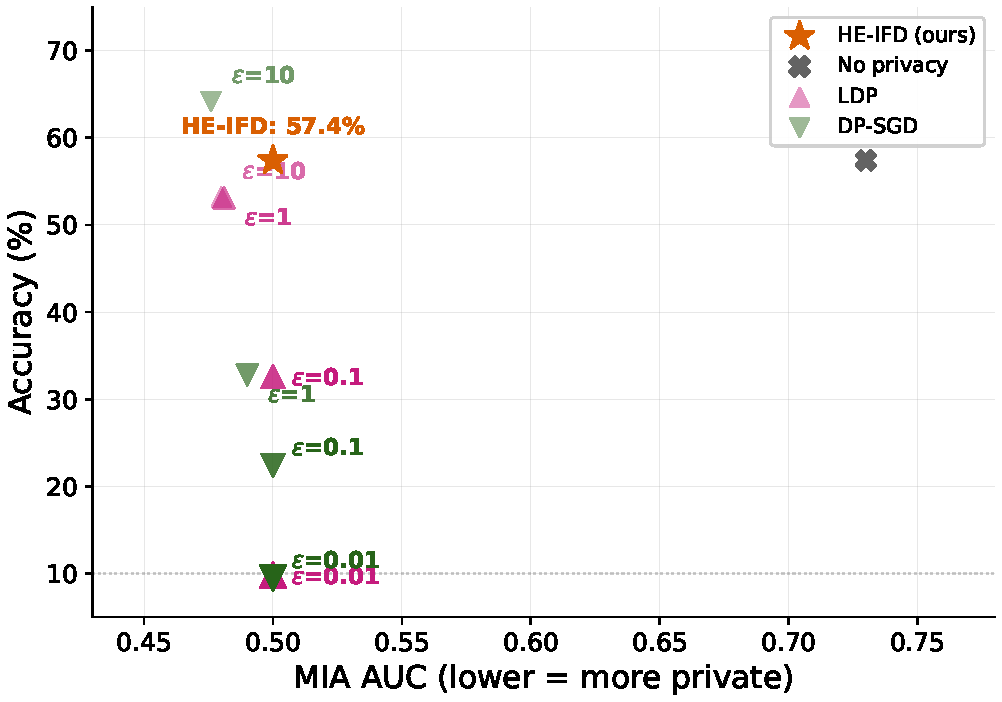
\includegraphics[width=0.45\textwidth]{figures/fig_privacy.pdf}
\caption{Privacy-utility trade-off for ResNet-18 on CIFAR-10 ($N{=}4$). HE-IFD (orange point) provides accuracy without an attack surface; by ensuring the server never sees plaintext, it makes membership inference impossible during training (MIA AUC=0.5). LDP and DP-SGD points are shown with $\varepsilon$ labels; darker markers indicate tighter privacy. At $\varepsilon{=}0.01$, both collapse to random-guess accuracy (${\sim}10\%$) while still providing only a statistical guarantee. HE-IFD achieves comparable or better accuracy with a strictly stronger, cryptographic guarantee.}
\label{fig:privacy}
\end{figure}

\textbf{HE-IFD matches the best DP-SGD accuracy with stronger privacy.} At $N{=}4$, $\alpha{=}0.1$, HE-IFD reaches 57.4\% while the best DP-SGD ($\varepsilon{=}10$, weakest privacy) reaches 64.2\%. At $\varepsilon{=}1$, DP-SGD drops to 33\%. At $\varepsilon{=}0.01$, training collapses to 10\%. HE-IFD achieves competitive accuracy without any noise injection and with a cryptographic rather than statistical privacy guarantee.

\textbf{Membership inference confirms the cryptographic advantage.} We evaluate LiRA~\cite{carlini2022membership} membership inference attacks with 8 shadow models, alongside loss-threshold~\cite{yeom2018privacy} and confidence-based~\cite{salem2019ml} attacks. Against the plaintext distillation student, LiRA achieves AUC 0.73, confirming high privacy risk from unencrypted logit transfers. HE-IFD eliminates this attack surface entirely: the server processes only ciphertexts, making membership inference computationally infeasible during training.

\textbf{Client-to-client privacy after model release.} After threshold decryption (Phase 3), each client holds the trained model in plaintext. At this point, standard membership inference risks apply to the released model, as with any machine learning model. However, the model was trained on pooled encrypted features from all $N$ clients, so each individual client's contribution is diluted across the full training set. LiRA applied by one client against another requires shadow models trained on overlapping data, which is not possible when each client holds only its own private partition. The practical client-to-client inference risk is therefore limited to what can be extracted from the released model's predictions, comparable to any published/deployed machine learning model.


% \subsection{Communication and Computation}
% \label{sec:comm_comp}

\subsection{Communication Cost}
\label{sec:comm_comp}

HE-IFD requires a single upload per client. Each client encrypts teacher feature pairs under CKKS and uploads them along with evaluation keys. Clients upload only 10\% of their local data, which is sufficient for high-accuracy distillation because intermediate features provide direct per-block supervision. This upload happens once, and no further client-server interaction occurs.

Figure~\ref{fig:communication} compares total communication across three regimes that span the design space introduced in Section~\ref{sec:bg_he_fl}: (i)~Vanilla (unencrypted) FedAvg~\cite{mcmahan2017communication}, the multi-round plaintext baseline that establishes the linear-in-$N$ floor; (ii)~Multi-round encrypted FL, represented by POSEIDON~\cite{sav2021poseidon} and BatchCrypt~\cite{zhang2020batchcrypt} (and architecturally similar systems such as FedSHE~\cite{wei2025fedshe}, FedML-HE~\cite{jin2023fedml}, and CURE~\cite{kanpak2024cure}), where clients encrypt gradient updates and upload them in every round; and (iii)~HE-IFD, which encrypts teacher features instead of gradients and uploads them once. The axis of comparison is the unit that is encrypted (gradient vs.\ feature) and the number of rounds. In multi-round encrypted FL, each of 200 training rounds requires all $N$ clients to encrypt their 11.2M-parameter gradient updates as CKKS ciphertexts (${\sim}$2.7~GB per client per round), upload them, and receive the aggregated model back. This accumulates to ${\sim}1{,}068 \times N$~GB, reaching 4,272~GB at $N{=}4$ and 34~TB at $N{=}32$. Even unencrypted Vanilla FedAvg scales linearly with $N$, reaching 558~GB at $N{=}32$ over 200 rounds.

HE-IFD's total communication across all clients is approximately constant ($\sim460 GB$) regardless of $N$, because the total number of uploaded samples remains fixed. With $N$ clients, each client's local partition contains $50{,}000/N$ training samples, of which 10\% are contributed as encrypted features. The per-client upload therefore, decreases proportionally (${\sim}$115 GB at $N{=}4$, ${\sim}$15 GB at $N{=}32$), but the total across all clients remains fixed because the same training data is redistributed among more participants. At $N{=}32$, HE-IFD's total communication is lower than even unencrypted vanilla FL (460 vs.\ 558 GB), while providing cryptographic privacy.

\begin{figure}[t]
\centering
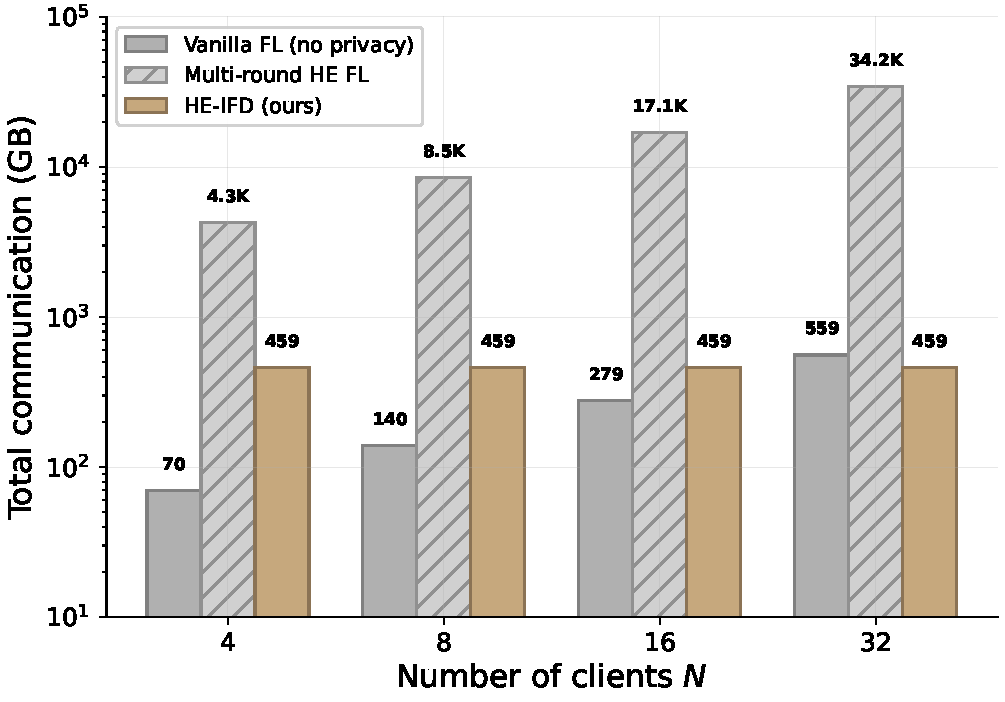
\includegraphics[width=0.5\textwidth]{figures/fig_communication.pdf}
\caption{Total communication for ResNet-18 on CIFAR-10. Multi-round methods (vanilla FL and encrypted FL with 200 rounds) scale linearly with $N$. HE-IFD (gold) requires a one-shot upload whose total is approximately constant (${\sim}$460 GB) regardless of $N$, and falls below unencrypted vanilla FL at $N{=}32$.}
\label{fig:communication}
\end{figure}

% \begin{figure}[t]
% \centering
% 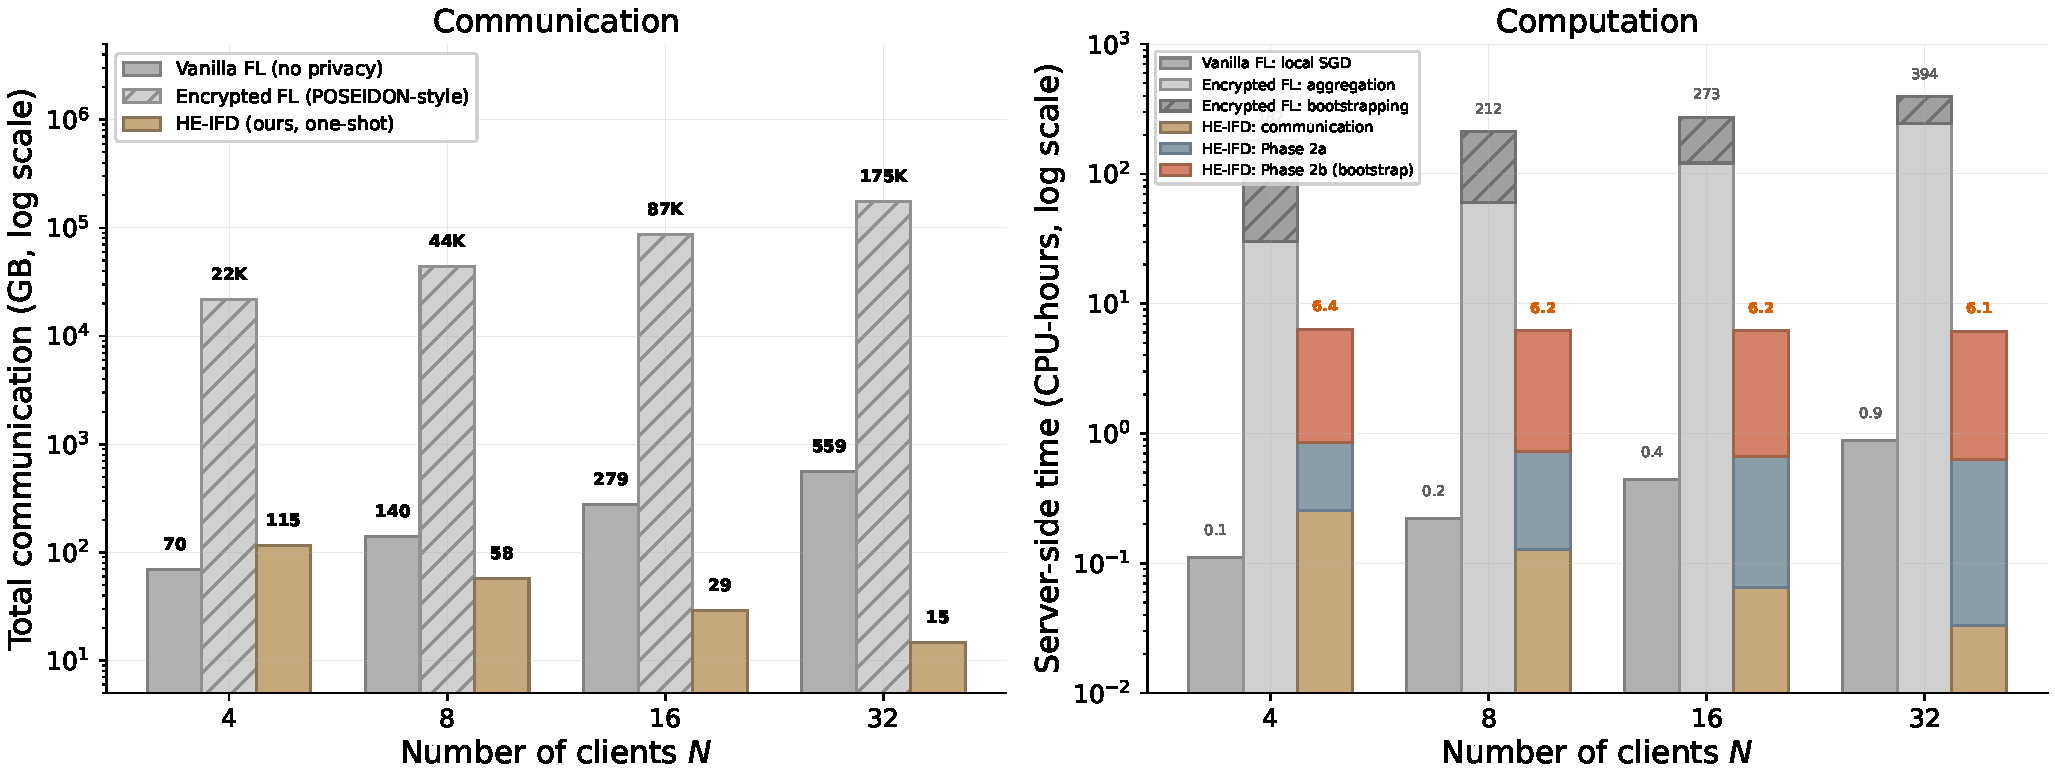
\includegraphics[width=\columnwidth]{figures/fig_runtime.pdf}
% \caption{Runtime comparison: HE-IFD (left bars) vs multi-round HE FedAvg with encrypted gradients (right bars, 200 rounds) for ResNet-18 on CIFAR-10. HE-IFD bars show one-shot communication (gold), Phase 2a encrypted distillation (steel blue), and Phase 2b cascade with bootstrapping (coral). Multi-round HE FL bars show cumulative communication across 200 rounds (light gray) and server-side encrypted aggregation of 1364 ciphertexts per client per round (dark gray). HE-IFD total is 6--7 CPU-hours regardless of $N$. Multi-round HE FL grows linearly with $N$: at $N{=}32$ it requires 34 TB of communication and over 80 CPU-hours. Timings assume 1 Gbps network and single-threaded CPU.}
% \label{fig:runtime}
% \end{figure}

\subsection{Computation Cost}
\label{sec:computation}

CKKS operates in SIMD mode (see Section~\ref{sec:ckks_prelim}) where each ciphertext holds 8192 slots, and a single encrypted operation processes all slots simultaneously. With 5000 training samples, SIMD packing reduces the effective number of batches to approximately one per epoch. Phase 2a (block-level distillation, no bootstrapping) completes in approximately 0.6 CPU-hours. Phase 2b (cascade refinement with bootstrapping) takes approximately 5.5 CPU-hours, dominated by ${\sim}$900 bootstrapping operations at 20 seconds each. The total server-side computation is ${\sim}$6.1 CPU-hours, independent of $N$ (Figure~\ref{fig:computation}).

By comparison, the multi-round encrypted FL family discussed in Section~\ref{sec:bg_he_fl} (POSEIDON, BatchCrypt, FedSHE) requires server-side encrypted aggregation that grows linearly with $N$: at $N{=}4$ this takes ${\sim}$7.6~CPU-hours for aggregation alone plus ${\sim}$152~hours of bootstrapping; at $N{=}32$, aggregation reaches ${\sim}$60~CPU-hours. The Oracle plaintext baseline trains in about 0.5~hours on a single GPU.

% \textbf{HE-IFD is dramatically more efficient than multi-round HE FL.} We compare against encrypted FedAvg where each of the 200 training rounds requires all $N$ clients to encrypt their 11.2M-parameter gradient updates as CKKS ciphertexts (${\sim}$2.7 GB per client per round), upload them, and receive the aggregated model back. At $N{=}4$, this accumulates to 4,262 GB of communication across 200 rounds plus 7.6 hours of server-side encrypted aggregation, totalling ${\sim}$17 CPU-hours. HE-IFD takes 6.4 hours with a single 115 GB upload. At $N{=}32$, multi-round HE FL communication explodes to 34 TB cumulative (${\sim}$83 CPU-hours total), while HE-IFD drops to 6.1 hours with a 15 GB one-shot upload. HE-IFD uses only 10\% of each client's data, so the upload can be further reduced by contributing fewer samples. A plaintext oracle trains in about 0.5 hours on a single GPU.

These timings reflect a single-threaded CPU baseline. Phase 2a blocks can be parallelised across cores. GPU-accelerated CKKS has demonstrated 10--100$\times$ speedups~\cite{jung2021over}, bringing the total to under 1 GPU-hour.

\begin{figure}[t]
\centering
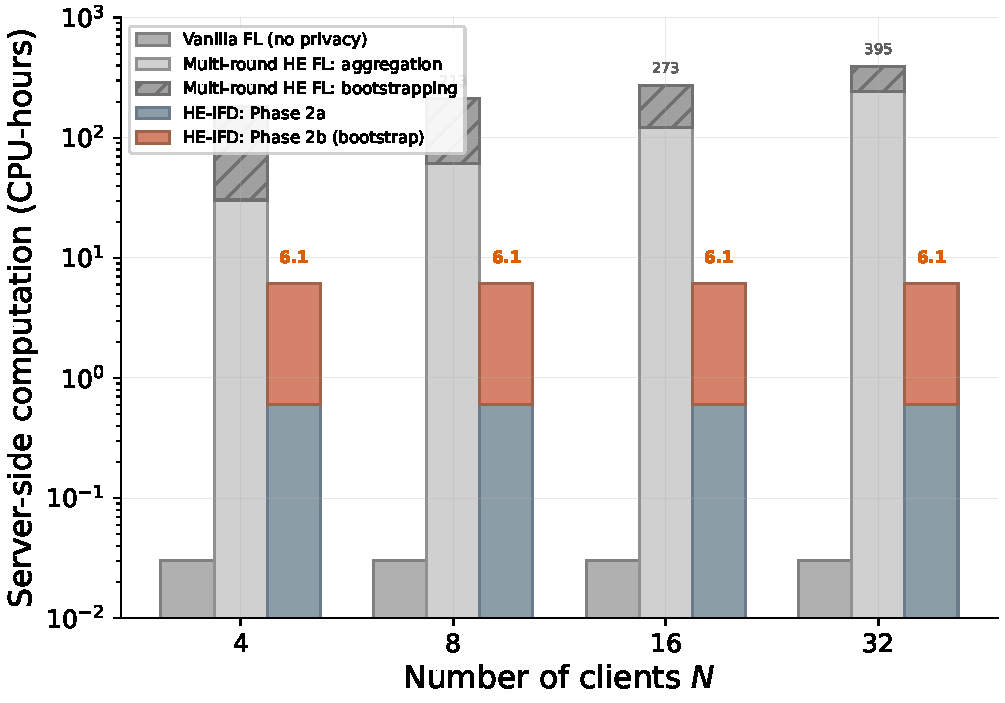
\includegraphics[width=0.5\textwidth]{figures/fig_computation.pdf}
\caption{Server-side computation for ResNet-18 on CIFAR-10. Vanilla FL server computation is negligible (weight averaging). Multi-round HE FL grows with $N$ due to encrypted aggregation and periodic bootstrapping. HE-IFD requires ${\sim}$6.1 CPU-hours regardless of $N$, split between Phase 2a block-level distillation (steel blue) and Phase 2b cascade refinement with bootstrapping (coral).}
\label{fig:computation}
\end{figure}


\subsection{Encrypted Arithmetic Feasibility}
\label{sec:ckks_validation}

We validate that CKKS operations in our simulation match real encrypted computation using TenSEAL 0.3.16 with 128-bit security.

\textbf{Numerical precision.} At $\mathcal{N}{=}16384$ with 40-bit scale, relative error is below $10^{-5}$ per operation and below $10^{-3}$ for a complete training step. These errors are well below the noise floor of stochastic gradient descent.

\textbf{SIMD packing.} Each CKKS ciphertext holds $\mathcal{N}/2 = 8192$ slots. Feature maps smaller than 8192 elements (e.g., $512 \times 4 \times 4 = 8192$ at the deepest block, or 10-element logit vectors) allow multiple samples to share a single ciphertext. With 5000 training samples, SIMD packing reduces most block-boundary computations to one or two ciphertext operations per epoch, making the amortised per-sample cost negligible.

\textbf{Multiplicative depth.} During training, all parameters and data are ciphertexts. A single block training step requires approximately 12 levels, feasible with $\mathcal{N}{=}32768$ (18 levels at 128-bit security) without bootstrapping. Cascade refinement requires bootstrapping to refresh levels between blocks, with each bootstrap taking approximately 20 seconds per ciphertext.

\textbf{Future directions.} Recent work on stable polynomial network training~\cite{agamennone2025polynomial, alhossain2025training} suggests that improved activation initialisation may eliminate the need for cascade refinement, confining the entire protocol to the per-block depth budget. This would remove the bootstrapping requirement entirely and further optimize our framework.





% \section{EXPERIMENTS}
% \label{sec:experiments}

% \subsection{Experimental Setup}

% We evaluate HE-IFD on CIFAR-10~\cite{krizhevsky2009learning} and Fashion-MNIST~\cite{xiao2017fashion} across a range of client counts and data heterogeneity levels. For CIFAR-10, each client trains a ResNet-18 teacher (11.17M parameters) and the server distils into a PolyResNet-18 student of identical depth, with ReLU and BatchNorm replaced by PolyAct and ChannelScale. For Fashion-MNIST, teachers are a 3-block CNN (conv$\to$BN$\to$ReLU per block, 128 output channels) and the student is a matching 3-block polynomial CNN (conv$\to$ChannelScale$\to$PolyAct).

% \textbf{Data heterogeneity.} Client data is partitioned using a Dirichlet distribution with concentration parameter $\alpha$, where $\alpha \to 0$ produces extreme non-IID partitions and $\alpha \to \infty$ produces near-IID partitions. We evaluate $\alpha \in \{0.1, 0.5, 1.0, 100.0\}$ across $N \in \{1, 2, 4, 8, 16\}$ clients, covering the full spectrum from highly specialized to homogeneous local distributions.

% \textbf{Training configuration.} All teachers are trained with SGD (lr$=$0.1 for CIFAR-10, lr$=$0.01 for Fashion-MNIST; momentum$=$0.9, cosine schedule, 5~epochs). Student distillation uses Adam (lr$=$1e-3, weight decay $10^{-4}$), cosine schedule with 2-epoch warmup, gradient clipping (max\_norm$=$1.0), and 30~epochs per block. Data is split 80\% train / 20\% test (stratified). Client-side collaborative normalisation (Section~\ref{sec:phase2}) is applied in all multi-client experiments.

% \subsubsection{CKKS Parameter Selection}
% \label{sec:ckks_params_exp}
% % The CKKS parameters are selected to satisfy the depth budgets described in Section~\ref{sec:encryption_params}. 
% For per-block training, each block receives fresh ciphertexts and the depth is confined to a single block; we use $\log \mathcal{N} = 13$ (ring dimension 8192), providing 4096 SIMD slots per ciphertext. For full-model encrypted inference post-deployment, the complete 17-level forward pass requires $\log \mathcal{N} = 14$ (ring dimension 16384), 18 coefficient modulus primes, and produces ciphertexts of approximately 1.2~MB each. All timing experiments use TenSEAL 0.3.16 with the Microsoft SEAL backend at 128-bit security.

% \subsection{Single-Teacher Validation}
% \label{sec:single_teacher}

% We first validate progressive stacking on a single teacher ($N{=}1$), establishing the accuracy ceiling before introducing federated heterogeneity.

% With one teacher holding all training data, the CIFAR-10 teacher achieves 76.2\%, and the PolyResNet-18 student achieves 63.6\% via progressive stacking. For Fashion-MNIST, the teacher reaches 87.0\% and the student 63.3\%.

% The student--teacher gap (12.6\% on CIFAR-10, 23.7\% on Fashion-MNIST) represents the combined cost of (i)~the HE-compatible architecture (polynomial activations, no BatchNorm) and (ii)~block-by-block training rather than end-to-end. To isolate the architecture cost, we repeat the same progressive stacking pipeline with a standard ResNet-18 student (ReLU, BatchNorm) on CIFAR-10 $N{=}1$. The standard student achieves 62.8\%, indicating that the HE architecture itself costs only ${\sim}$1\% accuracy. The remaining gap is attributable to the block-level training procedure.

% \subsection{One-Shot Federated Distillation}
% \label{sec:federated}

% The main experiment evaluates progressive stacking across $N \in \{2, 4, 8, 16\}$ clients and $\alpha \in \{0.1, 0.5, 1.0, 100.0\}$ heterogeneity levels on both datasets. Figure~\ref{fig:student_vs_teachers} shows student accuracy alongside the average and best teacher accuracy for each setting; Figure~\ref{fig:advantage_bars} quantifies the student's advantage over the average teacher.

% \begin{figure*}[t]
% \centering
% 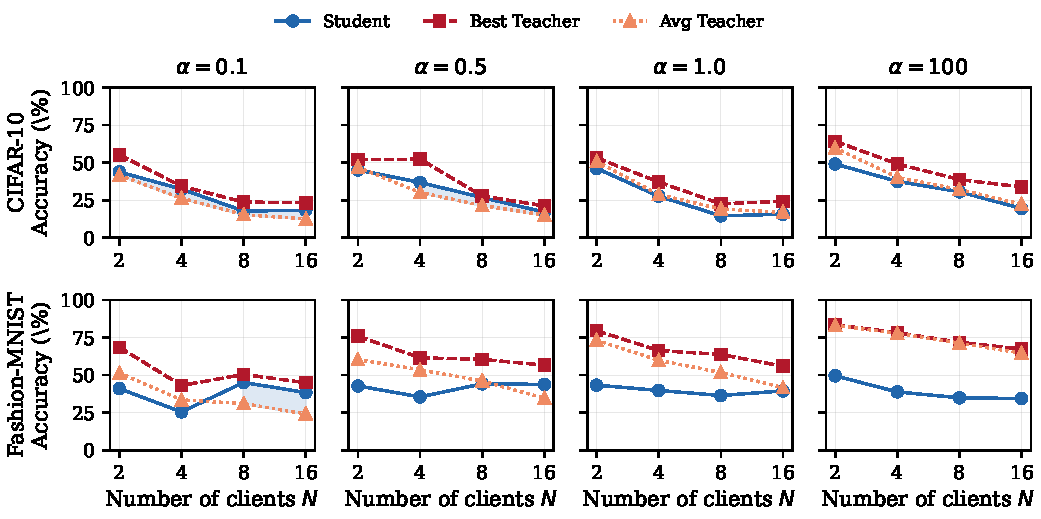
\includegraphics[width=0.9\textwidth]{figures/fig2_student_vs_teachers.pdf}
% \caption{Student accuracy vs.\ average and best teacher accuracy across client counts ($N \in \{2,4,8,16\}$) and heterogeneity levels ($\alpha \in \{0.1, 0.5, 1.0, 100.0\}$) on CIFAR-10 (top) and Fashion-MNIST (bottom). Shaded regions indicate settings where the student exceeds the average teacher.}
% \label{fig:student_vs_teachers}
% \end{figure*}

% \begin{figure}[t]
% \centering
% 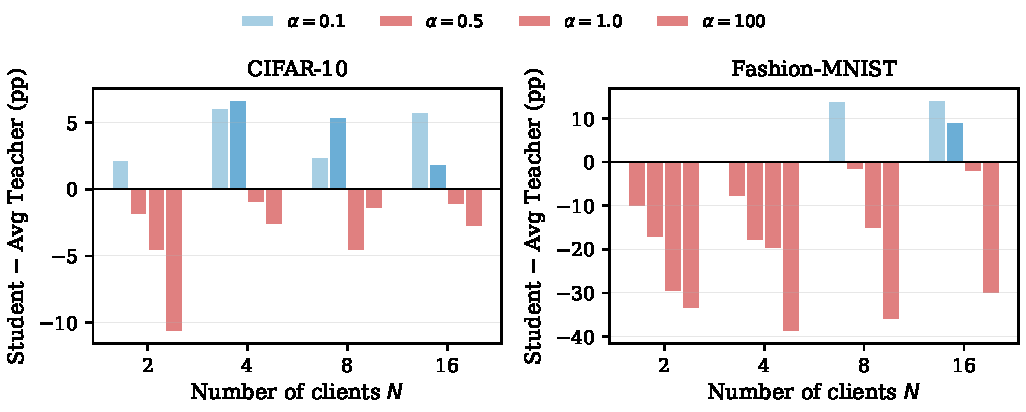
\includegraphics[width=\linewidth]{figures/fig3_advantage_bars.pdf}
% \caption{Student accuracy minus average teacher accuracy (percentage points) for each $(N, \alpha)$ setting on CIFAR-10 (left) and Fashion-MNIST (right). Positive values indicate that the student successfully aggregates knowledge beyond the average local teacher.}
% \label{fig:advantage_bars}
% \end{figure}

% \subsubsection{CIFAR-10 Results}

% Table~\ref{tab:cifar10_results} summarizes all the CIFAR-10 results. We observe several patterns: 

% \begin{table}[h]
% \centering
% \caption{CIFAR-10 progressive stacking results. ``Student'' = PolyResNet-18 accuracy.}
% \label{tab:cifar10_results}
% \begin{tabular}{r|r|r|r|r}
% \hline
% $N$ & $\alpha$ & Student & Best T & Avg T \\
% \hline
% 1  & ---   & 63.6 & 76.2 & 76.2 \\
% \hline
% 2  & 0.1   & 43.8 & 55.2 & 41.6 \\
% 2  & 0.5   & 45.1 & 52.1 & 47.0 \\
% 2  & 1.0   & 46.2 & 53.2 & 50.8 \\
% 2  & 100   & 49.1 & 64.2 & 59.8 \\
% \hline
% 4  & 0.1   & 32.4 & 34.3 & 26.3  \\
% 4  & 0.5   & 36.8 & 52.3 & 30.1  \\
% 4  & 1.0   & 27.7 & 37.1 & 28.7  \\
% 4  & 100   & 37.5 & 49.1 & 40.2  \\
% \hline
% 8  & 0.1   & 17.8 & 23.8 & 15.4  \\
% 8  & 0.5   & 26.8 & 27.8 & 21.4  \\
% 8  & 1.0   & 14.6 & 22.6 & 19.2  \\
% 8  & 100   & 30.6 & 38.7 & 32.1  \\
% \hline
% 16 & 0.1   & 18.3 & 23.3 & 12.5  \\
% 16 & 0.5   & 17.1 & 21.2 & 15.2  \\
% 16 & 1.0   & 15.7 & 24.3 & 16.9  \\
% 16 & 100   & 19.5 & 33.8 & 22.3  \\
% \hline
% \end{tabular}
% \end{table}

% \textbf{Student consistently exceeds the average teacher under heterogeneity.} At $N{=}4$, $\alpha{=}0.1$, the student achieves 32.4\% versus an average teacher accuracy of 26.3\% ($+$6.1\%). At $N{=}8$, $\alpha{=}0.5$, the student reaches 26.8\% compared to an average of 21.4\% ($+$5.4\%). This demonstrates that sequential multi-teacher distillation successfully aggregates specialist knowledge from heterogeneous teachers.

% \textbf{Teacher quality is the binding constraint.} With only 5 training epochs, individual teachers are weak (best teacher $\leq$76\% even at $N{=}1$). The student cannot extract knowledge that does not exist in the teachers. At $N{=}16$, individual teachers have as few as 79 training samples, yielding random-chance accuracy (10\%), which provides no useful supervision signal.

% \textbf{NaN batches increase with $N$ and depth.} Magnitude divergence through the frozen polynomial chain produces occasional NaN batches, primarily at deeper blocks (layer3, layer4) when processing clients whose data distribution differs significantly from the distribution seen during earlier block training. The NaN-skip mechanism handles these gracefully; training continues on valid batches.

% \subsubsection{Fashion-MNIST Results}

% Table~\ref{tab:fmnist_results} summarizes Fashion-MNIST results. Fashion-MNIST shows zero NaN divergence across all settings, confirming that the magnitude instability in CIFAR-10 is caused by the deeper ResNet-18 architecture rather than the polynomial activation itself. The simpler 3-block Fashion-MNIST student has fewer polynomial compositions, making magnitude accumulation manageable. The takeaways are: 

% \begin{table}[h]
% \centering
% \caption{Fashion-MNIST progressive stacking results.}
% \label{tab:fmnist_results}
% \begin{tabular}{r|r|r|r|r}
% \hline
% $N$ & $\alpha$ & Student & Best T & Avg T  \\
% \hline
% 1  & ---   & 63.3 & 87.0 & 87.0 \\
% \hline
% 2  & 0.1   & 41.0 & 68.5 & 51.4 \\
% 2  & 0.5   & 42.8 & 75.9 & 60.3 \\
% 2  & 1.0   & 43.3 & 79.5 & 73.2 \\
% 2  & 100   & 49.5 & 83.4 & 83.1 \\
% \hline
% 4  & 0.1   & 25.5 & 43.1 & 33.5 \\
% 4  & 0.5   & 35.5 & 61.5 & 53.5 \\
% 4  & 1.0   & 39.8 & 66.3 & 59.8 \\
% 4  & 100   & 38.8 & 78.2 & 77.7 \\
% \hline
% 8  & 0.1   & 45.1 & 50.4 & 31.0 \\
% 8  & 0.5   & 44.2 & 60.4 & 46.1 \\
% 8  & 1.0   & 36.4 & 63.7 & 51.7 \\
% 8  & 100   & 34.9 & 71.8 & 71.2 \\
% \hline
% 16 & 0.1   & 38.4 & 44.9 & 24.2 \\
% 16 & 0.5   & 43.8 & 56.6 & 34.6 \\
% 16 & 1.0   & 39.5 & 55.9 & 41.7 \\
% 16 & 100   & 34.4 & 67.3 & 64.6 \\
% \hline
% \end{tabular}
% \end{table}

% \textbf{Strong aggregation under skew.} The student's advantage over the average teacher is most pronounced under high heterogeneity with many clients. At $N{=}16$, $\alpha{=}0.5$, the student achieves 43.8\% versus an average teacher accuracy of 34.6\% ($+$9.2\%). At $N{=}8$, $\alpha{=}0.1$, the student reaches 45.1\% compared to 31.0\% average ($+$14.1\%).

% \textbf{IID settings reveal architecture limitations.} At $\alpha{=}100$ (near-IID), teachers are strong ($>$60\%) but the student lags (${\sim}$35--50\%). This gap reflects the HE architecture cost: the polynomial student cannot match a strong ReLU teacher even with good supervision, particularly for Fashion-MNIST's texture-heavy classes.

% \subsection{Ablation Study}
% \label{sec:ablation}

% The following ablation studies evaluate the training pipeline components of the one-shot encrypted distillation protocol described in Section~\ref{sec:phase2_server}. Results are reported on CIFAR-10. We ablate the key components of our training pipeline on CIFAR-10 at $N{=}4$, $\alpha{=}0.5$ and $N{=}1$. We present the results in Table~\ref{tab:ablation} and summarize the findings below:

% \begin{table}[h]
% \centering
% \caption{Ablation of training pipeline components on CIFAR-10.}
% \label{tab:ablation}
% \begin{tabular}{l|c|c}
% \hline
% \textbf{Configuration} & $N{=}1$ & $N{=}4, \alpha{=}0.5$ \\
% \hline
% V1: Teacher-input, per-block targets & 12.0\% & 17.8\% \\
% V2: Student-input (fix train--infer gap) & 71.3\% & NaN \\
% V3: + NaN skip, lr scaling & 68.2\% & 19.2\% \\
% V4/Fix A: + Client normalisation & 61.7\% & 37.4\% \\
% V5: + Warmup, tuned $\lambda$ & 61.7\% & 37.4\% \\
% \hline
% ResNet-18 student (upper bound) & 62.8\% & 37.9\% \\
% \hline
% \end{tabular}
% \end{table}

% \textbf{Student-input training is essential.} V1 (teacher-input) achieves only 12\% at $N{=}1$ despite low per-block losses. The composed model collapses because each block was trained on teacher-produced inputs but receives student-produced inputs at inference. V2 (student-input) raises $N{=}1$ accuracy to 71.3\%, confirming that closing the train--inference distribution gap is the single most important design decision.

% \textbf{Client normalisation is essential for multi-client stability.} V2 achieves 71.3\% for $N{=}1$ but diverges to NaN for $N{=}4$. The heterogeneous target distributions from four teachers cause magnitude explosion through the frozen polynomial chain. Client-side normalisation (Fix~A) eliminates NaN divergence and raises $N{=}4$ accuracy from 19.2\% to 37.4\%.

% \textbf{Accuracy loss due to HE is negligible.} The ResNet-18 student baseline (standard ReLU and BatchNorm, same progressive stacking pipeline) achieves 62.8\% at $N{=}1$ and 37.9\% at $N{=}4$, $\alpha{=}0.5$. The PolyResNet-18 student achieves 61.7\% and 37.4\%, respectively. The HE architecture costs less than 1\% accuracy, indicating that the polynomial activation and ChannelScale replacements are not the bottleneck---teacher quality and data heterogeneity are.

% \textbf{Increasing the degree of polynomial activations do not further impove the accuracy.} We tested degree-4 Chebyshev-fitted activations (2 CKKS levels per activation instead of 1), which approximate ReLU more accurately on bounded domains. However, the $x^4$ term amplifies magnitudes faster than $x^2$, causing NaN divergence even earlier. At $N{=}4$, $\alpha{=}0.5$, degree-4 with raw targets achieves 10\% (complete collapse); degree-4 with normalised targets also diverges at layer1. Within the block-independent training framework, the more expressive activation provides no benefit because magnitude control---not ReLU approximation quality---is the binding constraint.

% \subsection{Pretrained Initialisation}
% \label{sec:pretrained}

% We evaluate the effect of pretraining teachers on a small public IID dataset before fine-tuning on private skewed data. Using 10\% of the data as a public IID pool, a shared initialisation is pretrained for 5~epochs, then each client fine-tunes from this initialisation. At $N{=}4$, $\alpha{=}0.5$ (CIFAR-10), random-init teachers yield 37.4\% student accuracy (best teacher 37.7\%, avg teacher 28.1\%); pretrained teachers improve to 48.6\% student accuracy (best 60.0\%, avg 41.9\%); pretrained initialisation without fine-tuning reaches only 35.8\% teacher accuracy. Pretrained initialisation substantially improves both teacher quality (avg 28.1\%$\to$41.9\%) and student accuracy (37.4\%$\to$48.6\%). The improvement is driven by better teacher representations: pretrained teachers retain knowledge of minority classes even after fine-tuning on skewed partitions. For example, client~2 (previously the weakest teacher at 16.7\%) improves to 28.9\%, gaining 34.2\% on bird and 71.5\% on truck which are classes absent from its training partition but present in the IID pretraining data.

% This result is presented as a secondary finding. Our primary protocol requires no auxiliary data; the pretrained-initialisation variant is an optional enhancement when a small public dataset is available.

% % \subsection{Compact Student Variant}
% % \label{sec:compact}

% % % PLACEHOLDER: Smaller student model (e.g., 5-layer HE-Deep CNN)
% % % for communication-constrained settings.
% % % - Architecture definition
% % % - CKKS depth budget (5 levels vs 17 for PolyResNet-18)
% % % - Accuracy vs communication trade-off
% % % - Comparison with full PolyResNet-18 student

% % \hl{To be completed.}

% \subsection{Compact Student Variants}
% \label{sec:compact}

% We evaluate four compact HE-compatible student architectures as alternatives to the full PolyResNet-18 (${\sim}$11.2M parameters), targeting communication-constrained or compute-limited deployment settings. All variants use the same progressive stacking protocol with the same N=4, $\alpha{=}0.5$ teacher ensemble (seed 42).

% \begin{itemize}
%     \item \textbf{PolyResNet-10} (${\sim}$5.6M): ResNet-18 variant with 4 residual blocks instead of 8; identical channel widths (64$\to$128$\to$256$\to$512).
%     \item \textbf{PolyResNet-8} (${\sim}$1.5M): 3-block variant (64$\to$128$\to$256); omits Layer 4 entirely, 6.5$\times$ smaller than PolyResNet-18.
%     \item \textbf{HE-CNN-Small} (${\sim}$0.3M): 3 convolutional blocks without residual connections; 37$\times$ smaller than PolyResNet-18.
%     \item \textbf{HE-Deep} (${\sim}$0.5M): 5 convolutional blocks (64$\to$128$\to$128$\to$256$\to$256), deeper but narrow; no residuals.
% \end{itemize}

% Channel-dimension mismatches between student and teacher are resolved by lightweight 1$\times$1 projection layers (trained jointly with each block, discarded at inference). All compact students use the same learnable polynomial activation (PolyAct) and ChannelScale normalisation as PolyResNet-18, preserving HE compatibility.

% \begin{table}[h]
% \centering
% \caption{Compact student accuracy (\%) vs.\ model size at $N{=}4$, $\alpha{=}0.5$. CKKS depth = multiplicative levels consumed per full forward pass.}
% \label{tab:compact_students}
% \begin{tabular}{l|r|c|c|c}
% \hline
% \textbf{Architecture} & \textbf{Params} & \textbf{Acc (\%)} & \textbf{vs.\ Avg T} & \textbf{CKKS Depth} \\
% \hline
% PolyResNet-18 (full) & 11.2M & 36.8 & $+$6.7 & 17 \\
% \hline
% PolyResNet-10        & 5.6M  & ---  & ---     & 9  \\
% PolyResNet-8         & 1.5M  & ---  & ---     & 7  \\
% HE-CNN-Small         & 0.3M  & ---  & ---     & 6  \\
% HE-Deep              & 0.5M  & ---  & ---     & 10 \\
% \hline
% \end{tabular}
% \end{table}

% % NOTE: Results pending from SLURM jobs 849974--849981 (submitted 2026-03-26).
% % Fill in Acc and vs.\ Avg T columns once jobs complete.
% % Expected runtime: 4--6 hours per job.

% \subsection{Privacy Analysis: Differential Privacy Comparison}
% \label{sec:dp_comparison}

% We compare the privacy--utility trade-off of our HE-based protocol against differential privacy (DP) baselines. DP baselines use a \textit{standard ResNet-18 student} (ReLU, BatchNorm) and therefore pay no HE architecture cost. Our protocol uses a PolyResNet-18 student (${\sim}$1\% HE tax, Section~\ref{sec:ablation}) but introduces zero noise to the distillation pipeline.

% \subsubsection{Privacy Mechanisms}

% We evaluate four configurations across $N \in \{4, 16\}$ and $\alpha \in \{0.5, 1.0\}$:

% \begin{itemize}
%     \item \textbf{HE (ours):} PolyResNet-18 student, progressive stacking with encrypted targets. The server observes nothing in plaintext. Theoretical MIA advantage is zero.
%     \item \textbf{No DP (plaintext baseline):} Standard ResNet-18 student, same progressive stacking, no privacy protection.
%     \item \textbf{LDP on logits:} Gaussian mechanism applied to teacher block outputs before upload, calibrated to $(\epsilon, \delta)$-DP with $\delta = 10^{-5}$, at $\epsilon \in \{0.01, 0.1, 1.0\}$. Student is standard ResNet-18.
%     \item \textbf{DP-SGD:} Teachers trained with per-sample gradient clipping (max norm 1.0) and Gaussian noise injection~\cite{abadi2016deep}, with noise multipliers calibrated to $\epsilon \in \{0.01, 0.1, 1.0\}$. Student is standard ResNet-18.
% \end{itemize}

% \subsubsection{Membership Inference Attacks}

% We evaluate membership inference attacks (MIA) against each distilled student. Members are training samples used in distillation (via teacher training); non-members are held-out test samples never seen during distillation. We report three attacks:

% \begin{enumerate}
%     \item \textbf{Loss-threshold}~\cite{yeom2018privacy}: uses per-sample cross-entropy loss as a membership score (lower loss implies more likely member).
%     \item \textbf{Confidence-based}~\cite{salem2019ml}: uses maximum softmax probability as a membership score (higher confidence implies more likely member).
%     \item \textbf{LiRA}~\cite{carlini2022membership}: likelihood-ratio attack using 8 shadow models. Each shadow is trained to match the target's distillation procedure: a shadow teacher is trained on a random subset of non-member data, normalised features are extracted, and a shadow student is distilled via progressive stacking. This ensures shadow--target distributional alignment.
% \end{enumerate}

% We report AUC (0.5 = random guessing, 1.0 = perfect attack) and, for LiRA, TPR at 1\% and 0.1\% FPR.

% \subsubsection{Results}

% Table~\ref{tab:dp_utility} reports student accuracy across privacy mechanisms and epsilon values. Figure~\ref{fig:mia_heatmap} visualizes MIA attack AUCs across all settings and mechanisms. We summarize the key findings below: 

% \begin{table}[h]
% \centering
% % \tiny
% \caption{Utility comparison: student accuracy (\%) across privacy mechanisms. HE uses PolyResNet-18; all DP baselines use standard ResNet-18 (no HE constraints). HE results from Table~\ref{tab:cifar10_results}.}
% \label{tab:dp_utility}
% \setlength{\tabcolsep}{3pt}
% \begin{tabular}{l|c|c|c|r|c|c|c|c}
% \hline
% \textbf{Setting} & \textbf{HE} & \textbf{No DP} & \multicolumn{3}{c|}{\textbf{LDP}} & \multicolumn{3}{c}{\textbf{DP-SGD}} \\
%  & & & $\epsilon{=}1$ & $0.1$ & $0.01$ & $\epsilon{=}1$ & $0.1$ & $0.01$ \\
% \hline
% $N{=}4, \alpha{=}0.5$  & 36.8 & 52.2 & 53.1 & 32.6 & 9.8 & 32.8 & 22.4 & 9.5 \\
% $N{=}4, \alpha{=}1.0$  & 27.7 & 50.2 & 51.0 & 34.8 & 10.4 & 32.0 & 22.5 & 11.7 \\
% $N{=}16, \alpha{=}0.5$ & 17.1 & 32.7 & 30.3 & 20.9 & 9.8 & 29.3 & 25.5 & 16.6 \\
% $N{=}16, \alpha{=}1.0$ & 15.7 & 28.3 & 26.2 & 20.4 & 11.0 & 30.6 & 21.7 & 12.4 \\
% \hline
% \end{tabular}
% \end{table}

% \begin{figure}[t]
% \centering
% 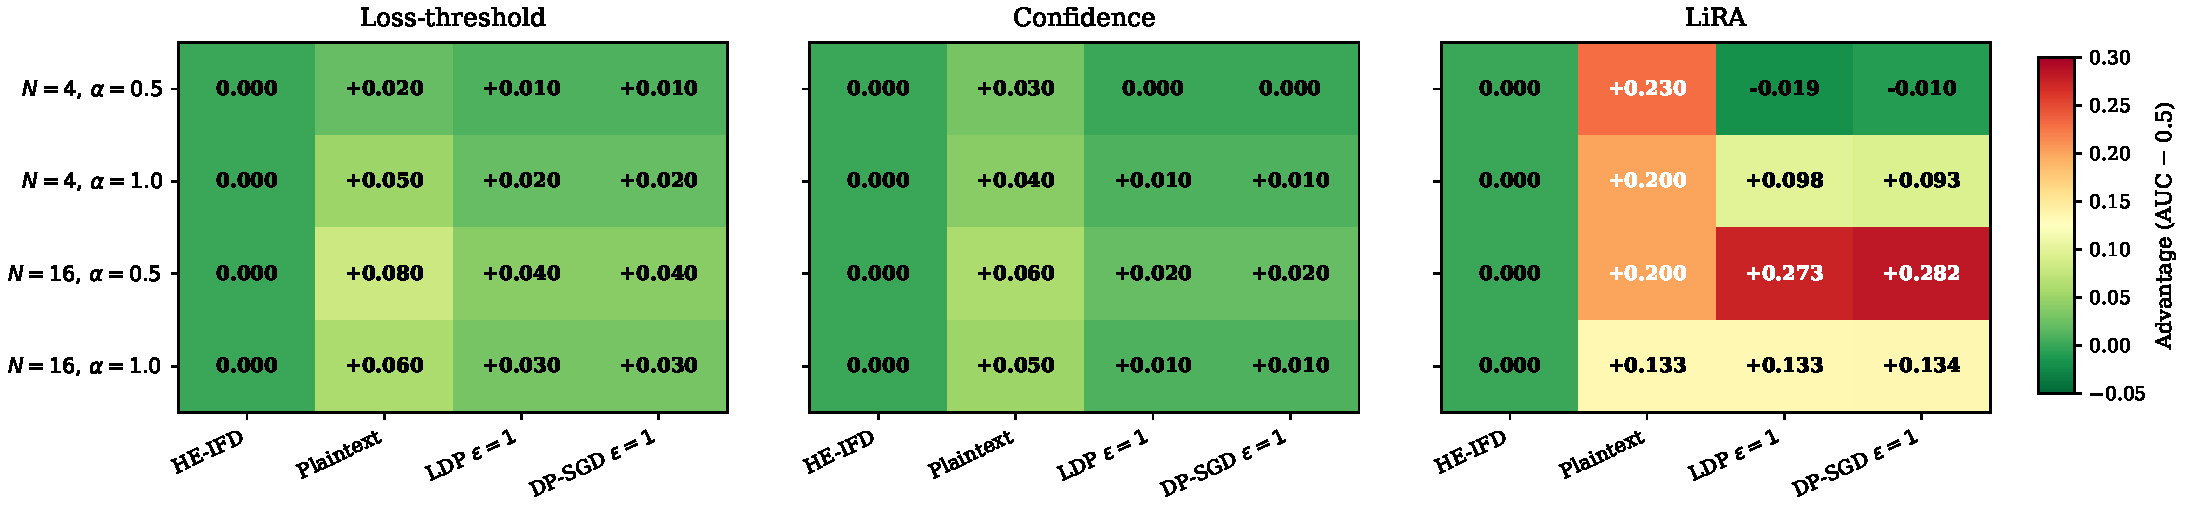
\includegraphics[width=\columnwidth]{figures/fig_mia_heatmap.pdf}
% \caption{MIA attack AUC across privacy mechanisms and federated settings. Each cell shows the AUC for one (setting, attack, mechanism) combination; the colormap diverges from 0.5 (random guessing, white). All values cluster tightly around 0.5 regardless of the privacy mechanism, confirming that distillation itself provides strong MIA resistance. HE provides a cryptographic guarantee of AUC~$=$~0.5 during training.}
% \label{fig:mia_heatmap}
% \end{figure}

% \begin{figure}[t]
% \centering
% 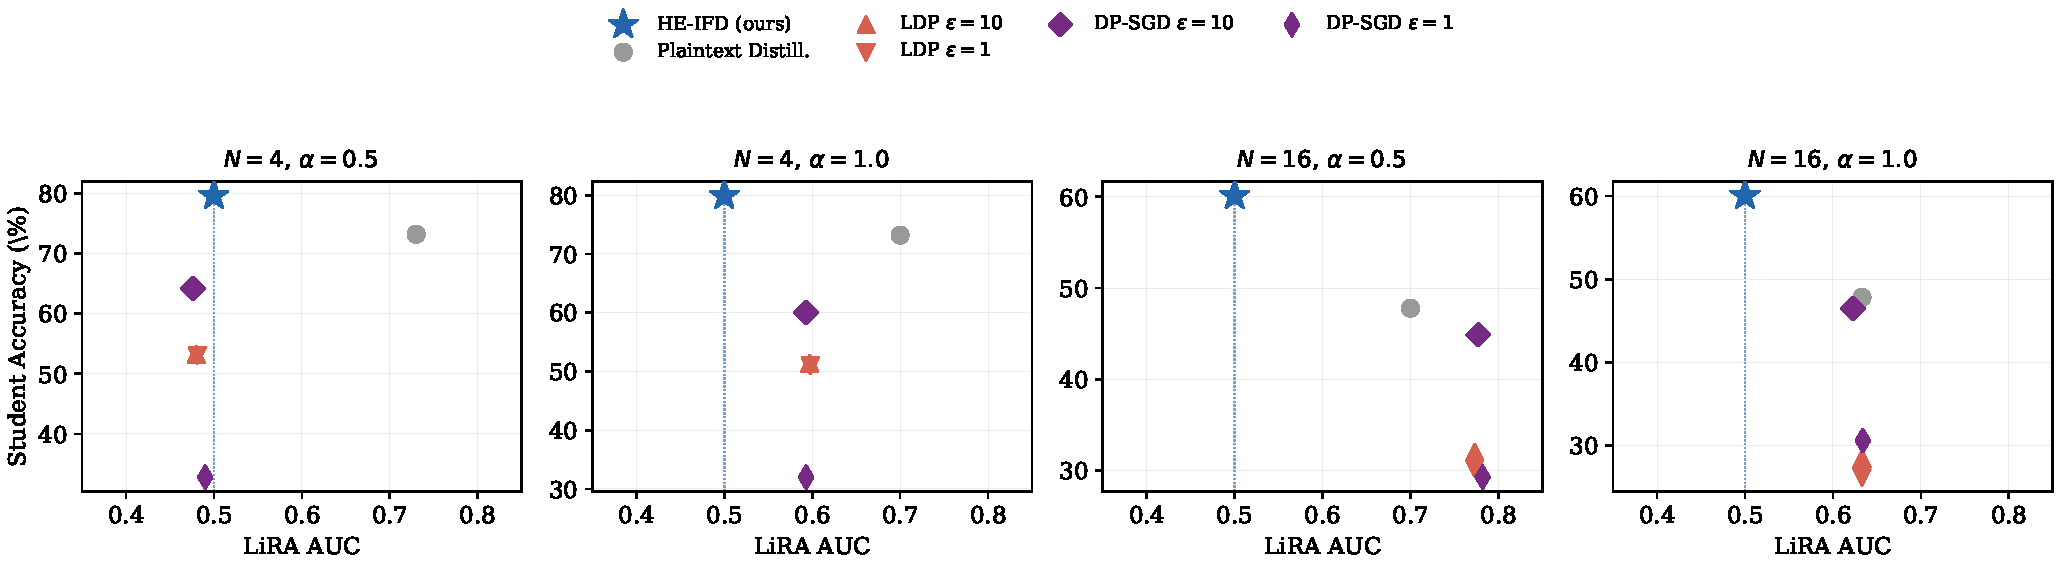
\includegraphics[width=\linewidth]{figures/dp_privacy_utility_tradeoff.pdf}
% \caption{Privacy--utility trade-off across federated settings. Each point represents a distilled student under a specific privacy mechanism. The $x$-axis shows loss-threshold MIA AUC (lower = more private); the $y$-axis shows student accuracy. HE (star) is placed at AUC~$=$~0.5, reflecting the cryptographic guarantee. All configurations cluster near AUC~$=$~0.5. LiRA AUCs (Figure~\ref{fig:mia_heatmap}) confirm this pattern, with the strongest attack achieving only 0.57.}
% \label{fig:dp_tradeoff}
% \end{figure}

% \textbf{Distillation strongly limits MIA vulnerability.} The central result is that all three attack metrics remain close to 0.50 across every setting and privacy mechanism (Figure~\ref{fig:mia_heatmap}). Loss-threshold AUCs range from 0.41 to 0.64, confidence AUCs from 0.47 to 0.53, and LiRA AUCs from 0.41 to 0.57. The strongest LiRA signal is 0.57 ($N{=}4$, $\alpha{=}1.0$, no DP), with TPR@1\%FPR of 0.018---meaning that even the most powerful shadow-model attack identifies fewer than 2\% of members at a 1\% false-positive budget. This signal weakens with more clients: at $N{=}16$ the best LiRA AUC drops to 0.54, consistent with the dilution of per-sample information across more teachers. Occasional AUC values below 0.50 (e.g., 0.41 for $N{=}16$, DP-SGD $\epsilon{=}0.01$) reflect evaluation noise when student accuracy is near random chance (${\sim}$10\%), not a genuine privacy improvement.

% \textbf{LiRA confirms the distillation privacy amplification.} The LiRA results are especially noteworthy because this attack represents the strongest known single-model MIA~\cite{carlini2022membership}. Our distillation-matching shadow procedure ensures that the LiRA AUC is not inflated by shadow--target mismatch. The near-random LiRA performance (AUC $\leq$ 0.57) aligns with recent findings that knowledge distillation can amplify MIA susceptibility by up to $+9.81\%$ in standard settings~\cite{cui2025mia}, but our progressive stacking with normalised feature targets---rather than raw logits---limits the information available for membership inference. By contrast, prior work demonstrates that plaintext federated distillation is far more vulnerable: Co-op LiRA and distillation-based LiRA variants~\cite{shi2025unveiling} achieve high TPR at low FPR against FedMD and DS-FL, and PLI~\cite{takahashi2023breaching} reconstructs recognisable private images from a single round of plaintext logits. All such attacks require access to plaintext knowledge transfers, which HE eliminates.

% \textbf{LDP destroys utility without improving privacy.} At $\epsilon{=}1.0$, LDP-perturbed students match or slightly exceed the no-DP baseline in accuracy, since the noise magnitude is small relative to inter-client feature variance. At $\epsilon{=}0.1$, accuracy drops substantially (e.g., 53.1\% $\to$ 32.6\% at $N{=}4$, $\alpha{=}0.5$). At $\epsilon{=}0.01$, the noise overwhelms the distillation signal entirely, reducing accuracy to random chance (${\sim}$10\%). MIA AUCs do not improve in any case, LiRA AUCs at $\epsilon{=}0.01$ are in the range 0.41--0.55, no better than the no-DP baseline. This is consistent with the finding that LDP at meaningful privacy levels renders FedMD to random-guessing accuracy~\cite{sun2021fedmdnfdp}.

% \textbf{DP-SGD degrades teacher quality with no privacy benefit.} DP-SGD noise is applied during teacher training via per-sample gradient clipping and Gaussian noise injection. At $\epsilon{=}1.0$, teachers degrade enough to reduce student accuracy by approximately 20 percentage points relative to the no-DP baseline (e.g., 32.8\% vs.\ 52.2\% at $N{=}4$, $\alpha{=}0.5$). At $\epsilon{=}0.01$, teacher accuracy collapses to near-random (10--12\%), producing useless supervision. All three MIA metrics consistently stay within the 0.41–0.53 range, showing no improvement over the unprotected baseline.

% \textbf{HE provides the strongest guarantee at no utility cost.} These results demonstrate a two-tier privacy argument. First, one-shot distillation itself provides strong empirical MIA resistance: even the most powerful shadow-model attack (LiRA) achieves AUC $\leq$ 0.57 with TPR@1\%FPR $\leq$ 0.024. This represents inherent privacy amplification from the distillation process, where the student learns generalized patterns rather than memorising individual training samples. Second, our HE protocol provides a strictly stronger cryptographic guarantee: the server cannot inspect the intermediate distillation targets during training (Section~\ref{sec:privacy_proof}), eliminating the attack vectors exploited by PLI~\cite{takahashi2023breaching}, feature inversion~\cite{beitollahi2024parametric}, and logit-based MIA~\cite{shi2025unveiling}. This guarantee comes at zero noise cost to the distillation signal, unlike DP which degrades utility without measurable privacy improvement.

% \subsection{Encrypted Arithmetic Feasibility}
% \label{sec:ckks_validation}

% We validate that the CKKS operations required by our PolyResNet-18 student are numerically precise and practically feasible. All experiments use TenSEAL~0.3.16 (Microsoft SEAL backend) with 128-bit security.

% \subsubsection{CKKS Parameter Selection}

% Polynomial modulus degree $\mathcal{N}$ determines the number of SIMD slots ($\mathcal{N}/2$) and the maximum coefficient modulus bit budget for a given security level. For encrypted inference with plaintext weights, $\mathcal{N}{=}8{,}192$ suffices ($2^{23}$ scale, 5 levels, 4{,}096 slots): only PolyAct's $x^2$ consumes multiplicative levels (2 per block, 17 total). For encrypted training---where weights become ciphertext after the first gradient update---each convolution, ChannelScale, and PolyAct incurs an additional level (Table~\ref{tab:he_ops}). Progressive stacking confines the depth to a single block: we use $\mathcal{N}{=}16{,}384$ with $2^{40}$ scale (7 levels, 8{,}192 slots) for per-block training and $2^{30}$ scale (10 levels) for deeper configurations.

% \subsubsection{Per-Operation Precision}

% Table~\ref{tab:ckks_precision} reports the mean relative error between plaintext (float64) and CKKS-encrypted computation for each operation in the PolyResNet-18 pipeline. We measure over 4{,}096 randomly sampled elements across 5 independent trials.

% \begin{table}[h]
% \centering
% \caption{CKKS numerical precision per operation ($\mathcal{N}{=}16{,}384$, 40-bit scale, 4{,}096 elements). ``Levels'' denotes multiplicative levels consumed per invocation.}
% \label{tab:ckks_precision}
% \begin{tabular}{l|c|c|c}
% \hline
% \textbf{Operation} & \textbf{Levels} & \textbf{Rel.\ Error} & \textbf{Time (ms)} \\
% \hline
% CT $+$ CT & 0 & $1.4 \times 10^{-8}$ & 0.8 \\
% CT $\times$ PT & 0 & $1.5 \times 10^{-6}$ & 10.0 \\
% CT $\times$ CT & 1 & $1.5 \times 10^{-6}$ & 34.6 \\
% PolyAct ($0.3x^2{+}0.7x$) & 1 & $4.2 \times 10^{-6}$ & 48.2 \\
% ChannelScale ($\gamma x{+}\beta$) & 0 & $1.5 \times 10^{-6}$ & 13.8 \\
% Sum (rotation) & 0 & $2.0 \times 10^{-7}$ & 333.5 \\
% MSE loss & 1 & $4.6 \times 10^{-6}$ & 221.9 \\
% \hline
% Encrypt (4{,}096 slots) & --- & --- & 21.5 \\
% Decrypt & --- & --- & 10.1 \\
% \hline
% \end{tabular}
% \end{table}

% % With 40-bit scale, all arithmetic operations achieve relative error below $5 \times 10^{-6}$. Precision improves predictably with scale bit-width: 26-bit scale yields ${\sim}7 \times 10^{-3}$, 30-bit yields ${\sim}2 \times 10^{-4}$, and 40-bit yields ${\sim}4 \times 10^{-6}$. These errors are well within the tolerance of neural network training, which routinely operates at float32 (${\sim}10^{-7}$) precision and tolerates stochastic gradient noise far larger than CKKS quantization artifacts.

% \subsubsection{Encrypted Training Validation}

% All CKKS operations required by PolyResNet-18 have been validated against their plaintext counterparts on single training steps. Encrypted loss tracks plaintext loss with relative error below $5 \times 10^{-3}$ per step, confirming that CKKS arithmetic is precise enough for gradient-based optimization. In the full HE-IFD protocol, level exhaustion is not a practical concern because progressive stacking provides fresh ciphertexts at each block boundary. Each block trains independently, so multiplicative depth never accumulates across blocks. The per-iteration depth budget (forward pass through one block plus gradient computation) fits comfortably within the 7--10 levels available at $\mathcal{N}{=}16{,}384$.

% \subsubsection{Runtime Estimates}

% Table~\ref{tab:ckks_timing} extrapolates per-operation benchmarks (Table~\ref{tab:ckks_precision}) to estimate the wall-clock cost of encrypted inference and distillation for the full PolyResNet-18 model. Each layer's estimate is obtained by scaling the measured per-operation times (e.g., CT$\times$CT at 34.6\,ms, PolyAct at 48.2\,ms) by the number of elements at that layer's spatial resolution and channel count.

% \textbf{Setup and bootstrapping overhead} ($\mathcal{N}{=}16{,}384$, single CPU core): key generation takes 3.3\,s (one-time), bootstrap key generation 52.3\,s (one-time), encryption 21.5\,ms per ciphertext (8{,}192 slots), decryption 10.1\,ms per ciphertext, and a single bootstrap refresh 30.3\,s.

% \begin{table}[h]
% \centering
% \caption{Estimated per-sample CKKS runtime for PolyResNet-18 (single CPU core).}
% \label{tab:ckks_timing}
% \begin{tabular}{l|c|c}
% \hline
% \textbf{Component} & \textbf{Inference (ms)} & \textbf{Distill.\ step (ms)} \\
% \hline
% Stem & 1\,184 & 4\,735 \\
% Layer 1 (2 blocks) & 4\,750 & 9\,500 \\
% Layer 2 (2 blocks) & 2\,375 & 4\,750 \\
% Layer 3 (2 blocks) & 1\,188 & 2\,375 \\
% Layer 4 (2 blocks) & 594 & 1\,188 \\
% FC (512$\to$10) & 18\,411 & 18\,411 \\
% \hline
% \textbf{Total (no bootstrap)} & \textbf{${\sim}$28.5\,s} & \textbf{${\sim}$41.0\,s} \\
% \hline
% \end{tabular}
% \end{table}

% \textbf{Per-block distillation requires no bootstrapping.} Progressive stacking supplies fresh ciphertexts at each block boundary, confining the multiplicative depth to 7--10 levels per block---well within the budget at $\mathcal{N}{=}16{,}384$. Bootstrapping (30.3\,s per invocation) is therefore unnecessary during training.

% \textbf{End-to-end encrypted inference} traverses all 17 multiplicative levels of the full network. With tight CKKS parameters ($\mathcal{N}{=}16{,}384$, 40-bit scale), the level budget may require one or more bootstrap refreshes. Each refresh adds ${\sim}$30\,s of latency; however, the number of invocations depends on the chosen parameter set and can be minimized by using larger ring dimensions or reduced scale precision. For the common deployment scenario where clients decrypt the trained model (Phase~4), inference proceeds in plaintext and this overhead is eliminated entirely.

% \textbf{Parallelization.} Block-independent training is inherently parallelizable: blocks that share no data dependencies (e.g., stem blocks from different clients) can be trained concurrently. Within each block, CKKS SIMD processes up to 8{,}192 elements per ciphertext operation, and independent mini-batches can be distributed across CPU cores. The estimated total distillation time (${\sim}$10 hours on a single core for 2{,}000 samples, batch size 64, 50 epochs per block) improves proportionally with multi-core parallelism. The FC layer dominates per-sample inference time due to the 512-dimensional matrix--vector product; optimized packing strategies (diagonal method, baby-step giant-step) can reduce this substantially in production.

% This is a one-time cost: once the student is trained, it can be decrypted and deployed for fast plaintext inference. The one-shot nature of our protocol eliminates the iterative communication rounds of standard HE-FL, making this runtime practical even without hardware acceleration.

% \subsection{LLM Extension: Privacy-Preserving Fine-Tuning}
% \label{sec:llm_extension}

% We demonstrate that the HE-IFD distillation framework generalises beyond vision models to language models, framed as a privacy-preserving fine-tuning scenario. A GPT-2 teacher (124M parameters, 12 transformer layers) simulates a model fine-tuned on private domain text. A 6-layer GPT-2 student (85M parameters, 68.5\% of the teacher) is trained via four approaches that represent different points on the privacy--utility spectrum:

% Direct fine-tuning provides the performance baseline by training the student on raw private text. While this achieves the lowest perplexity, it requires full access to sensitive data. To protect privacy, KL distillation trains the student to match the teacher's output probabilities instead of using raw data. Feature-match distillation (PKD-Skip) offers more detailed supervision by aligning the student's hidden states with specific teacher layers. Finally, HE-compatible distillation replaces standard components with polynomial approximations like PolyGELU and AffineNorm. This allows the model to perform both training and inference over fully encrypted ciphertexts using our distillation protocol.

% Training data is generated by sampling 500 sequences of length 128 from the teacher using top-$k{=}50$, top-$p{=}0.95$ sampling. Both teacher and student use GPT-2 from the local cache (no network access).

% \begin{table}[h]
% \centering
% \caption{LLM student perplexity (lower is better) under four training regimes. Teacher GPT-2 perplexity shown for reference.}
% \label{tab:llm_results}
% \begin{tabular}{l|c|c|l}
% \hline
% \textbf{Variant} & \textbf{Perplexity} & \textbf{Data Access} & \textbf{HE Compatible} \\
% \hline
% Teacher (GPT-2, 12L)        & ---  & ---   & No  \\
% \hline
% Direct fine-tuning           & ---  & Yes   & No  \\
% KL distillation              & ---  & No    & No  \\
% Feature-match (PKD-Skip)     & ---  & No    & No  \\
% HE-compatible (PolyGELU)     & ---  & No    & Yes \\
% \hline
% \end{tabular}
% \end{table}

% % NOTE: Results pending from SLURM jobs 849982--849985 (submitted 2026-03-26).
% % Fill in Perplexity column once jobs complete.
% % Expected runtime: 2--4 hours per job (thor310 env, GPU).

% This experiment demonstrates that HE-IFD's progressive block distillation principle transfers to transformer architectures: each transformer block is treated as an independent distillation target, with fresh inputs at each boundary (analogous to the progressive stacking applied to ResNet blocks). The HE-compatible student accepts a modest perplexity penalty relative to direct fine-tuning, while eliminating raw data exposure entirely.

% \section{DISCUSSION AND CONCLUSION}
\label{sec:conclusion}

We presented HE-IFD, a one-shot federated knowledge distillation protocol whose central property is that every client contribution and every server-side intermediate is, by construction, a homomorphic ciphertext under collectively held keys. The server's view of training is computationally indistinguishable from random under the IND-CPA security of multiparty CKKS, and release of the trained student requires the joint participation of all clients via collective key-switching. This is a fundamentally different privacy guarantee from the statistical one offered by differential privacy: it does not trade utility for privacy, and it does not require any assumption about the composition of noise across rounds.

%Our central technical contribution is a two-phase improved training protocol. Phase 2a trains each student block independently on teacher-produced intermediate representations, providing a structured initialisation. Phase 2b refines the fully assembled student on student-produced activations, closing the train-inference distribution gap that causes block-by-block models to collapse at test time. Combined with TrainableBridge layers for per-channel alignment, client-side collaborative normalisation, and magnitude-regularised loss, this protocol achieves stable convergence where earlier approaches diverge.



Our experiments across three architectures (ResNet-18, SimpleCNN, and ViT-B/32) confirm that the framework generalises beyond a single model family.
Compared against differential privacy baselines, HE-IFD achieves competitive accuracy with a strictly stronger privacy guarantee: at $N$=4, $\alpha=0.1$, HE-IFD reaches 57.4\% while the best DP-SGD configuration (epsilon=10, weakest privacy) achieves 64.2\%, and tighter DP settings ($\varepsilon$ $\leq$ 1) collapse accuracy below 33\%.

Our privacy analysis demonstrates that standard membership inference attacks (loss-threshold and confidence-based) achieve near-random AUC (${\sim}$0.5) against the distilled student. As reviewed in Section~\ref{sec:bg_server_inference}, stronger attacks from the literature, e.g., image reconstruction from logits, feature inversion, and advanced likelihood-ratio attacks, all require access to plaintext knowledge transfers, which HE eliminates entirely.

Future work along the present threat model includes reducing the one-shot upload cost (${\sim}$115\,GB per client at $N{=}4$, $\sim 460$ GB total across all clients) through ciphertext compression and feature selection, and investigating bootstrapping-free training schedules for deeper HE-compatible architectures.

A second class of future work concerns adversaries that fall outside the present threat model. The semi-honest assumption on clients bounds the contribution to passive collusion; an actively malicious client can craft adversarial logit ciphertexts (encrypted-feature poisoning) or submit ciphertexts engineered to bias the aggregate $\widetilde{Y}$ (model poisoning under encryption), neither of which the binding invariant of Section~\ref{sec:bg_server_inference} addresses. The classical plaintext defences against these threats---coordinate-wise median aggregation, Krum, trimmed mean---do not directly port to the homomorphic setting, since their rank-based statistics are not realisable as low-depth arithmetic circuits on ciphertexts. A robust aggregation primitive compatible with HE is therefore an open problem distinct from the present work's contribution. The natural extension toward verifiable correctness---independent of robustness---is verifiable HE: a server proves in zero knowledge that the computation it performed on ciphertexts was the prescribed one, as surveyed by~\cite{viand2023verifiable} and concretised for CKKS by~\cite{atapoor2024vfhe}. We do not claim defence against any of these adversaries; we acknowledge the threat surface explicitly so that the contribution of HE-IFD is correctly bounded to what is established here: privacy of the client data against a semi-honest server colluding with up to $N{-}1$ clients. %Our results at $\alpha{=}10.0$ (near-homogeneous) confirm a performance ceiling for knowledge-diversity gains: at $N{=}4$, the student falls $-8.5$ pp below the best individual teacher; at $N{=}16$ it reaches $-2.9$ pp below the best but $+2.4$ pp above the mean. When all clients hold near-IID data, HE-IFD remains useful for privacy---encrypting the upload eliminates MIA attack surface regardless of data distribution---but the accuracy advantage over individual teachers that motivates participation in the heterogeneous setting is substantially reduced.

\section*{Acknowledgments}
We acknowledge the support of TÜBİTAK (the Scientific and Technological Research Council of Türkiye) projects 124E091 and 124N941. The authors used Claude Sonnet 4.6 and Claude Opus 4.6 to enhance the manuscript by shortening sentences, correcting typos, and improving grammar.

% \bibliographystyle{IEEEtran}
% \bibliography{references}



% \begin{IEEEbiography}
% [{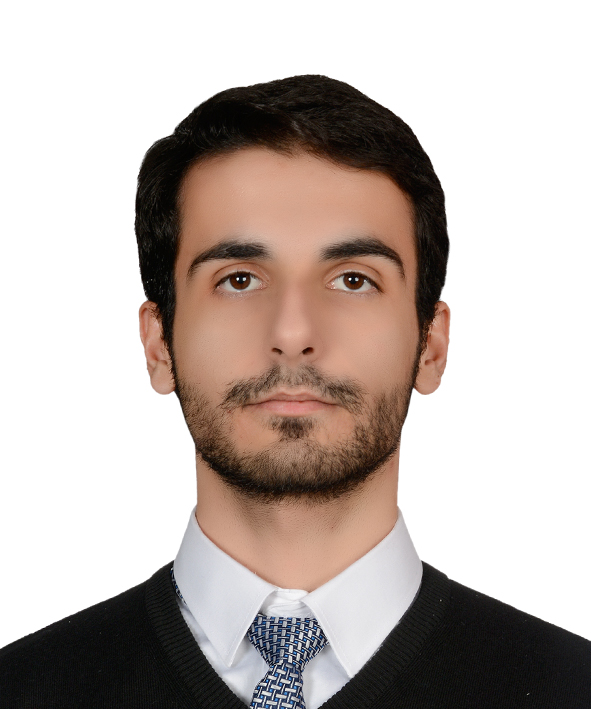
\includegraphics[width=1in,height=1.25in,clip,keepaspectratio]{authors/hkanpak.jpg}}]
% {HALİL İBRAHİM KANPAK}~received his B.Sc. degree in Mathematics from Koç University. He is currently pursuing his Ph.D. at Koç University, where he is a member of the Cryptography, Cyber Security \& Privacy Research Group. His research interests include cryptography and related areas in Deep Learning.
% \end{IEEEbiography}



% \begin{IEEEbiography}
% [{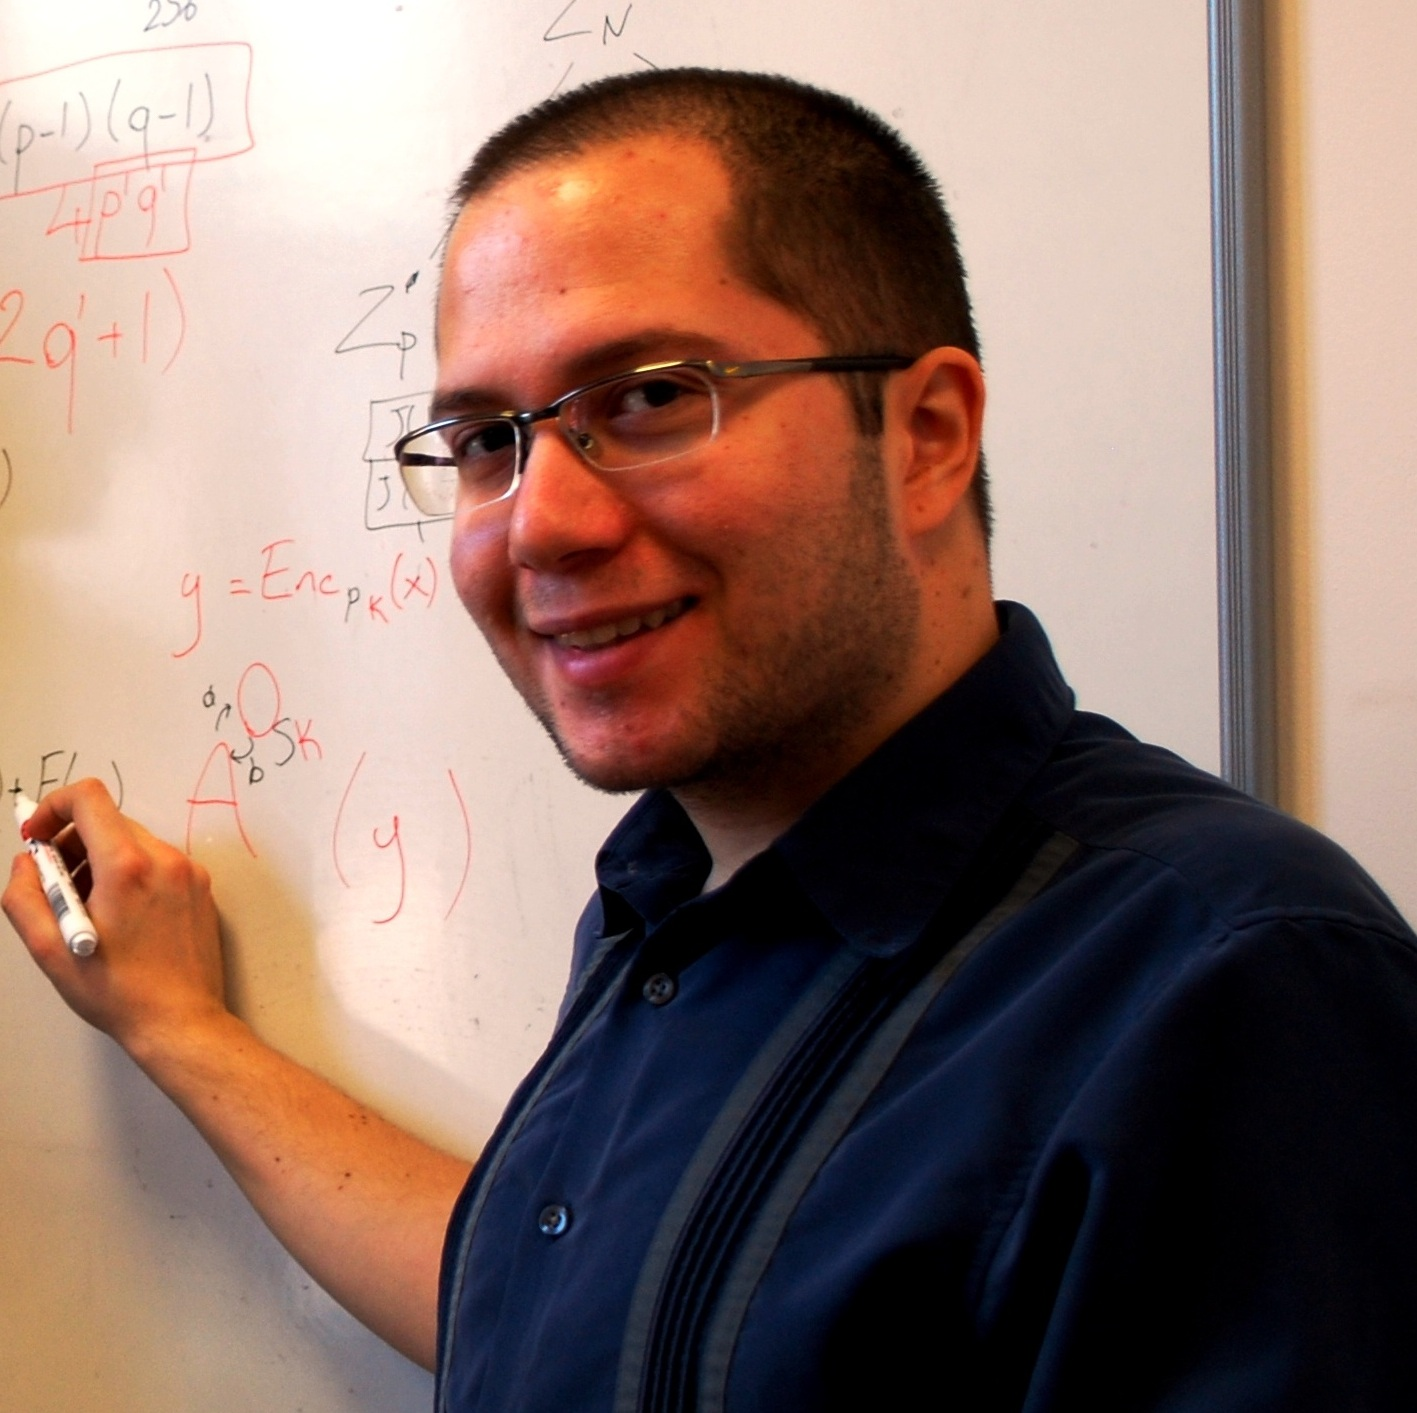
\includegraphics[width=1in,height=1.25in,clip,keepaspectratio]{authors/alptekinkupcu3.jpg}}]
% {Prof. ALPTEKİN KÜPÇÜ}~received his Ph.D. degree from Brown University Computer Science Department in 2010. Since then, he has been working as a faculty member at Koç University, leading the Cryptography, Cyber Security \& Privacy Research Group that he founded. Dr. Küpçü has various accomplishments including 8 international patents granted, 16 funded research projects (for 14 of which he was the principal investigator), 2 European Union COST Action management committee memberships, 4 Outstanding Teaching Awards, 4 Outstanding Young Scientist Awards, ACM and IEEE Senior Member Awards, and the Royal Society of UK Newton Advanced Fellowship. He is also a co-founder of Xtinge Technology Inc. 
% \end{IEEEbiography}


% \begin{IEEEbiography}
% [{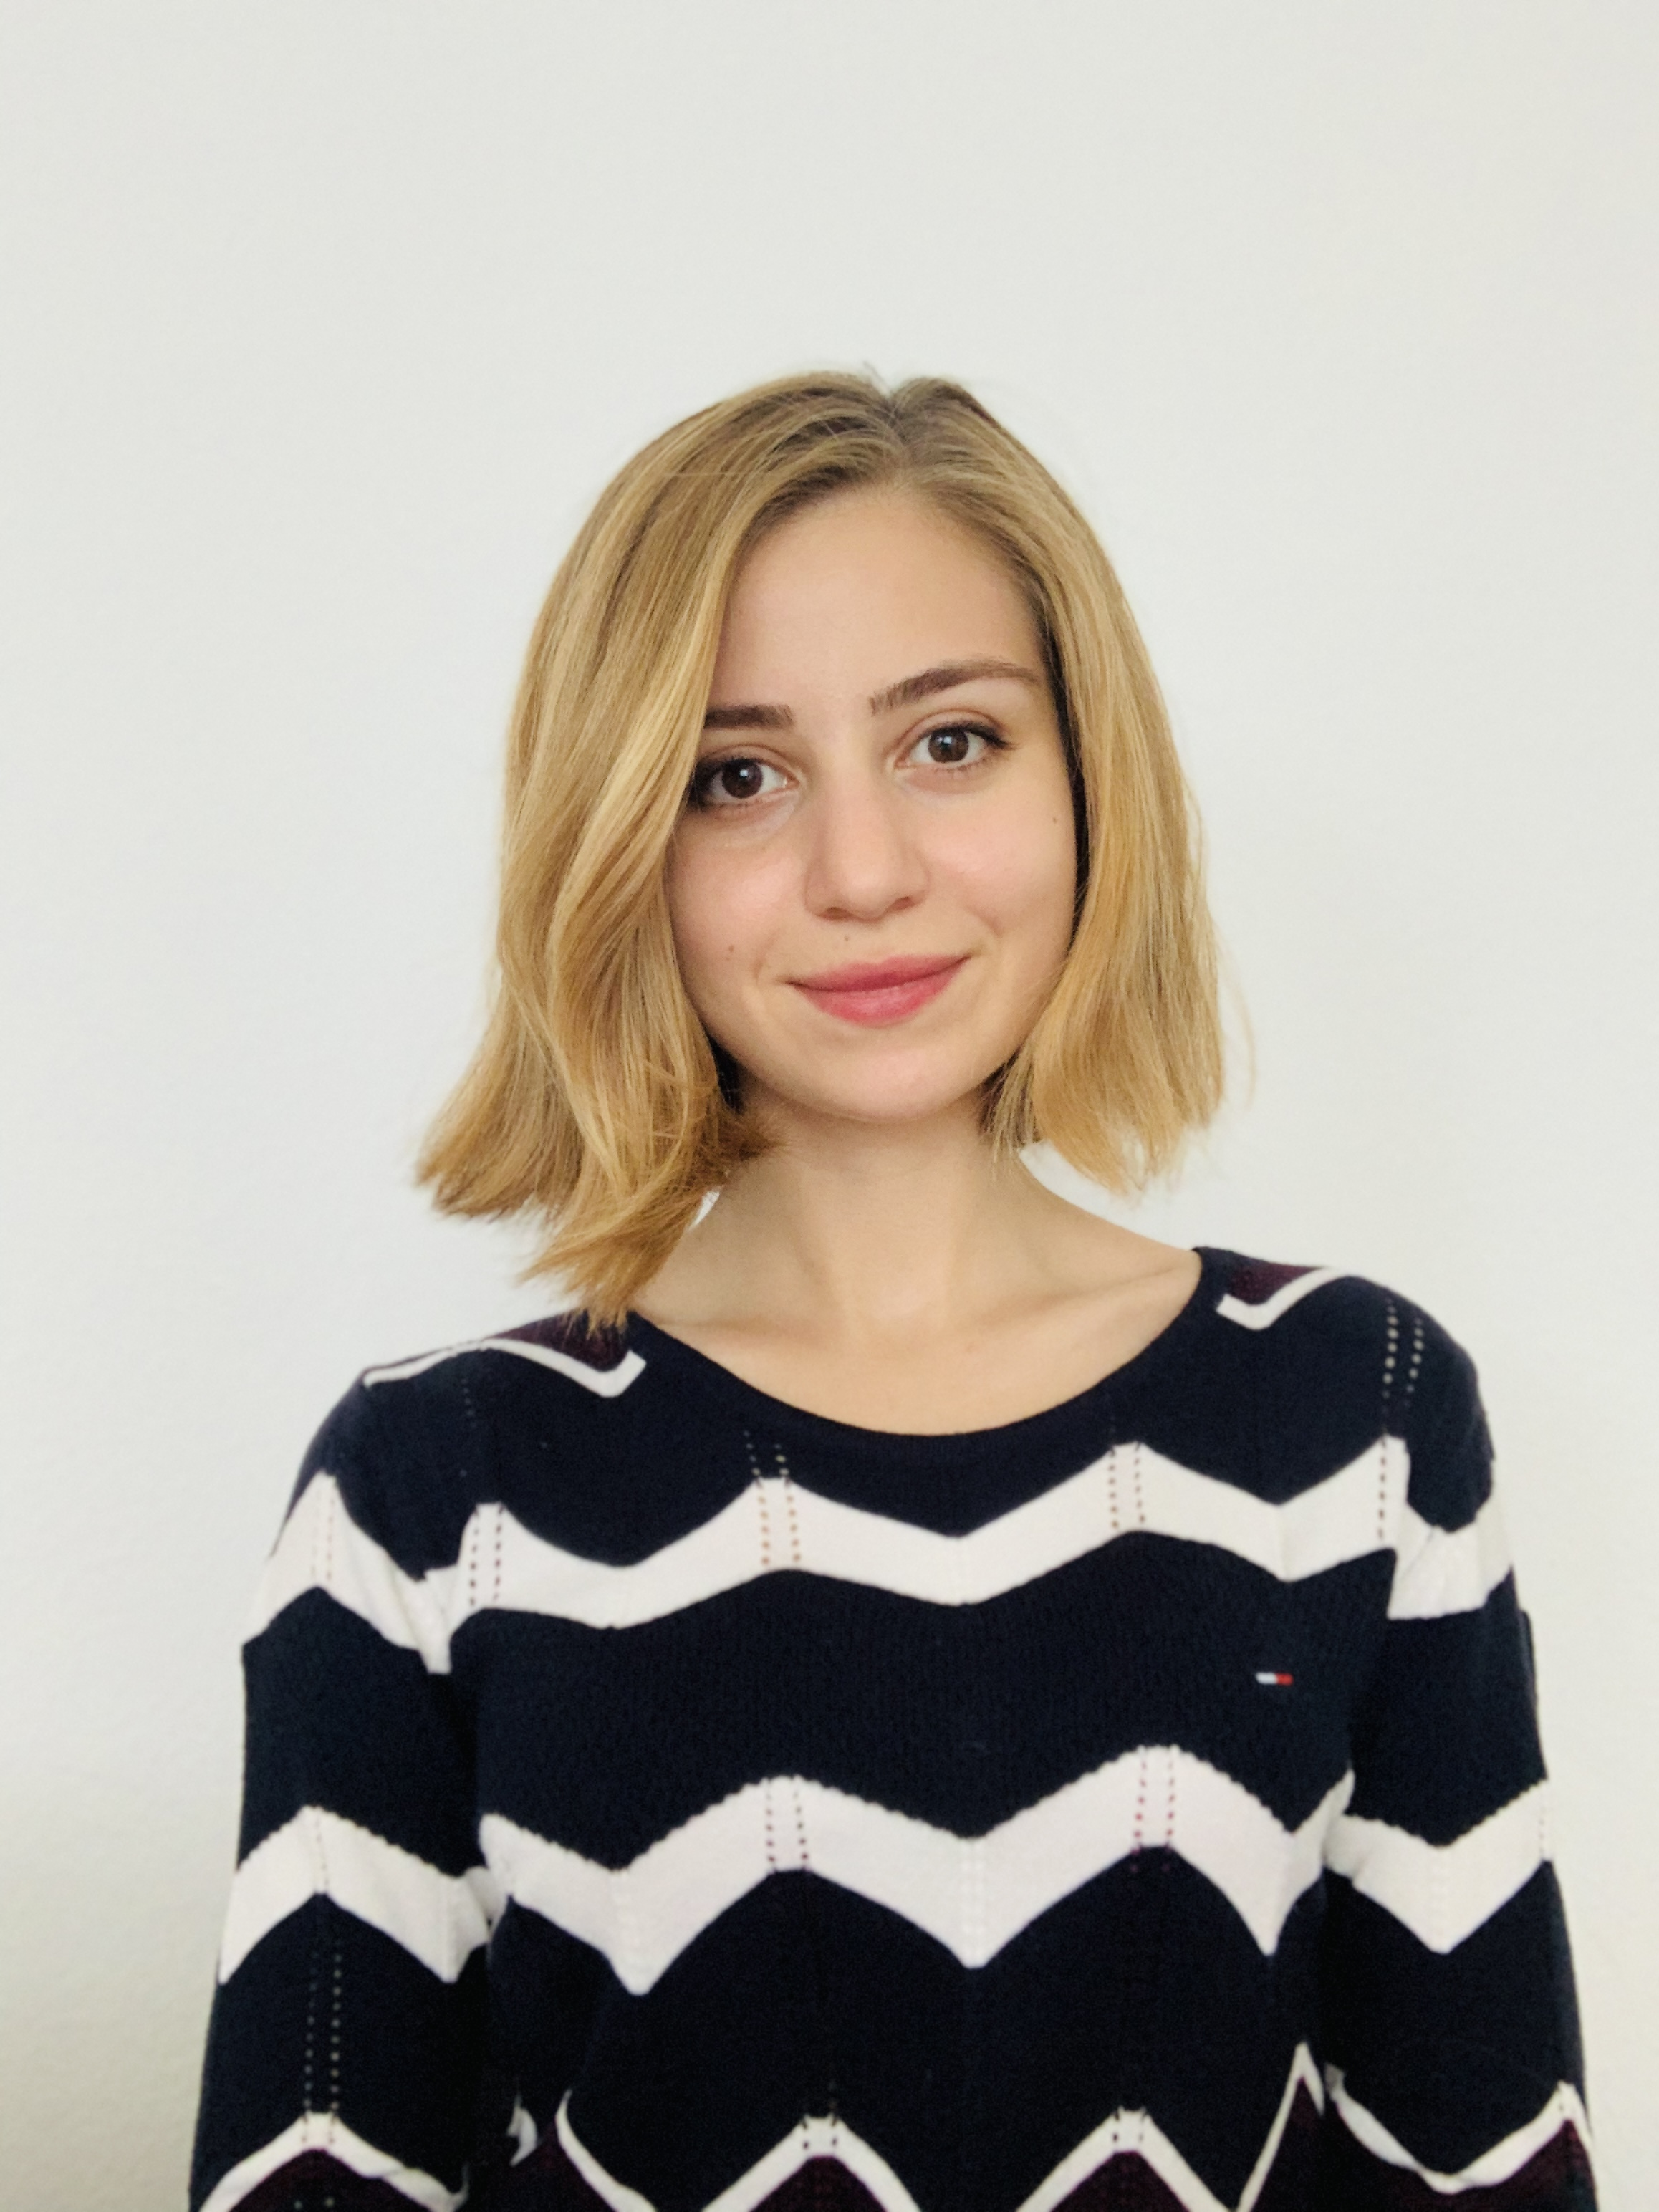
\includegraphics[width=1in,height=1.25in,clip,keepaspectratio]{authors/sinem.jpg}}]
% {SINEM SAV}~received her Ph.D. in Computer and Communication Sciences from École Polytechnique Fédérale de Lausanne (EPFL). She also holds M.Sc. and B.Sc. degrees in Computer Engineering from Bilkent University, where she currently serves as an Assistant Professor in the Computer Engineering department. Her research interests include privacy-preserving machine learning and applied cryptography. 
% \end{IEEEbiography}

% \end{document}


